\chapter*{}
\thispagestyle{empty}
\begin{vplace}[30]
\versal{O ESPECIALISTA}: Você não poderia ser mais breve?

\versal{O CANTOR}: Não.

Bertolt Brecht, O círculo de giz caucasiano (1948)
\end{vplace}

\part{Novos espaços}

\chapter{Los Angeles, 2019}

Em 1984, no já clássico \emph{Neuromancer}, de \index{Gibson, William}William Gibson, surgia a
primeira definição de ``ciberespaço''.\footnote{O termo propriamente
  dito já havia aparecido no conto {\slsc{Burning chrome}} (1982), do
  mesmo \index{Gibson, William}William Gibson, para designar uma máquina simuladora de
  realidade chamada ``Cyberspace Seven''. Antes disso, em 1968, a dupla
  dinamarquesa \index{Ussing, Susanne}Susanne Ussing e \index{Hoff, Carsten}Carsten Hoff havia criado uma
  instalação chamada {\slsc{Atelier Cyberspace}}.} O livro se passa num
futuro próximo e trata das agruras de um ex"-hacker que, tendo perdido
seu acesso à rede de computadores, perambula à deriva pelo submundo de
uma metrópole gigantesca em busca de uma forma de retornar ao mundo
virtual:

\begin{quote}
Ciberespaço. Uma alucinação consensual vivenciada diariamente por
bilhões de operadores autorizados, em todas as nações, por crianças que
estão aprendendo conceitos matemáticos\ldots{} uma representação gráfica de
dados abstraídos dos bancos de todos os computadores do sistema humano.
Uma complexidade impensável. Linhas de luz alinhadas no não"-espaço da
mente, aglomerados e constelações de dados. Como luzes da cidade, se
afastando\ldots{} (\versal{GIBSON}, 2016, p.~77).
\end{quote}

O romance é considerado a obra fundadora do \emph{cyberpunk}, um
subgênero de ficção científica surgido no início dos anos 1980 que, com
sua estética sombria e distópica, procurava contrapor"-se ao universo
luminoso de uma tecnologia triunfante presente em outras obras do
gênero. Se na série televisiva \emph{Jornada nas estrelas} (1966), a
tecnologia e a ciência estavam a serviço do homem e do Estado para a
conquista do espaço, no \emph{cyberpunk} o homem é subjugado por uma
tecnologia opressora dominada por grandes corporações às quais não tem
acesso.\footnote{{\slsc{Jornada nas Estrelas}} retrata as aventuras
  espaciais dos personagens a bordo da ``\scalebox{.8}{USS} Enterprise'', a principal
  nave da ``Frota Estelar'', uma armada diplomática a serviço da
  ``Federação Unida dos Planetas''.} Enquanto os personagens da série
descobrem novos planetas e mundos distantes, o cenário do
\emph{cyberpunk} é o submundo das grandes cidades do próprio planeta
Terra. É a representação de um futuro próximo que fracassa, uma distopia
caracterizada por uma ``high tech, low life'' (alta tecnologia, baixa
qualidade de vida). Seus personagens marginalizados vivem em cidades
futuristas decadentes, num mundo desprovido da regulação do Estado, e
não podem fazer muito mais do que lutar pela própria sobrevivência.

Apesar do limitado alcance filosófico como gênero literário, o
\emph{cyberpunk} com seu ``realismo sujo'' contém uma proposta bastante
original apoiada sobretudo numa potente estética visual. Os personagens
com próteses mecânicas, os robôs, os vagabundos, as cidades sob o céu
noturno de cores apocalípticas, a chuva incessante, as luzes neon em
meio à fumaça saída dos bueiros, os poderosos edifícios das corporações,
as referências à cultura oriental, tudo isso é mais significativo no
\emph{cyberpunk} do que uma proposta propriamente teórica.

O \emph{cyberpunk} surgiu na literatura, mas logo encontrou sua tradução
no cinema, notadamente com o filme \emph{Blade Runner} (1982), de \index{Scott, Ridley}Ridley
Scott.\footnote{Adaptado a partir do romance {\slsc{Androides sonham com
  ovelhas elétricas?}} (1968), de \index{Dick, Philip K.}Philip K. Dick.} Tanto \index{Gibson, William}Gibson quanto
\index{Scott, Ridley}Scott afirmam terem se inspirado na revista francesa de história em
quadrinhos de ficção científica \emph{Metal Hurlant}, sobretudo nos
desenhos de \index{Moebius}Moebius\footnote{Publicada nos Estados Unidos como
  {\slsc{Heavy Metal}.}} que, por sua vez, guardam evidente parentesco com
o filme \emph{Metropolis} (1927), de \index{Lang, Fritz}Fritz Lang, ícone do expressionismo
alemão. Tanto nos quadrinhos quanto nos filmes, a arquitetura das
cidades futuristas e os avanços da tecnologia são descritos com detalhe
e, não raro, têm mais importância do que o enredo dos personagens.
Quando se lembram de \emph{Blade Runner} as pessoas em geral se referem
mais ao cenário que à trama, mais aos aspectos estéticos do que aos
possíveis significados do filme.\footnote{Embora a análise de \index{Harvey, David}David
  Harvey seja uma grata exceção. Ver \scalebox{.8}{HARVEY}, David. {\slsc{Condição
    pós"-moderna: um estudo sobre a mudança cultural}}. São Paulo: Loyola,
  2014. pp.~277-289.}

\begin{figure}[!ht]
\centering
 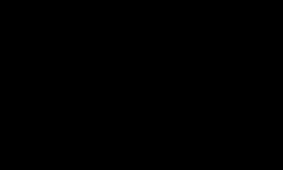
\includegraphics[width=85mm]{./imgs/im1.jpg}
\caption{\tiny{\Formular{Dan O'Bannon e \index{Moebius}Moebius. {\slsc{The long tomorrow}} (1976)}}}
\end{figure}

Após os créditos iniciais sobre fundo negro e um texto contextualizando
a história, surgem as palavras que nos situam no tempo e no espaço:
``Los Angeles, novembro de 2019''. Segue"-se a imagem aérea de uma cidade
imensa e noturna, com chaminés cuspindo fogo e carros voadores. A melancólica Los Angeles futurista é uma cidade de
edifícios altíssimos, criando verdadeiros desfiladeiros urbanos, cujo
fundo é habitado pelos seres humanos que rastejam pelas ruas insalubres
sem nunca ver a luz do sol. Dominando a cidade, o gigantesco complexo da
Tyrell Corporation, com sua forma piramidal lembrando um templo asteca.

Este é um mundo onde se venera o poder decadente do capital, com suas
propagandas luminosas gigantes a prometer um mundo de felicidade. Um
cenário inquietante e belo, como um pesadelo. Exerce um estranho
fascínio na medida em que é e não é o nosso mundo ao mesmo tempo; onde,
apesar dos avanços tecnológicos ainda não alcançados por nós, é possível
reconhecer o funcionamento da sociedade e a configuração das cidades.
Não é por acaso que tantas vezes nos vemos diante de algo ou de uma
situação que ``parece Blade Runner''.

No filme, as empresas de tecnologia concentram todo o poder político e
econômico, submetendo o Estado à sua vontade. Além disso, ocupam o lugar
da própria força divina, literalmente ``criando'' seres artificiais para
lhes servirem. Esses ``replicantes'' são androides fabricados à imagem e
semelhança dos homens, porém mais fortes e capazes, seres
tecnológicos destinados ao trabalho pesado. No entanto, os replicantes
de \index{Scott, Ridley}Ridley Scott, paradoxalmente, representam o último refúgio de uma
humanidade perdida, são os depositários do desejo de liberdade, de
afeto, de beleza e de aventura, enquanto os humanos propriamente são os
verdadeiros escravos submetidos ao poder corporativo. Perseguidos por
causa do potencial perigo que representam, lutam legitimamente pela
própria sobrevivência, reivindicando o direito à vida que lhes foi dada.
A rebeldia juvenil e violenta dos replicantes que se opõe ao sistema é a
atitude punk renovada, que encontra um novo lugar de existência no
universo ciberespacial de um futuro próximo.

Hoje, em 2019, percebemos que o filme antecipou com bastante sucesso
grande parte da realidade que nos rodeia. É verdade que hoje ainda não há carros voadores nem replicantes substituindo os humanos, mas é também verdade que a vida é cada vez mais controlada por imensas corporações tecnológicas, que as cidades são o duro cenário da injustiça social e que a natureza está entrando em colapso. Com os celulares que carregamos a todo momento, os
olhos fixos na tela, corpos e máquinas se fundem, criando ciborgues que
dependem de aparelhos para sobreviver. Mas o grande acerto do filme --- e
do \emph{cyberpunk} de uma forma geral --- diz respeito à organização do
sistema de poder. A tecnocracia, onde o poder se concentra na mão de
algumas empresas, suplantando o poder do Estado e impedindo a
participação dos cidadãos, é uma realidade. A nós, restam as migalhas do
sistema e a luta individual pela sobrevivência, como os personagens que
rastejam nas ruas chuvosas daquela cidade distópica.\footnote{É sintomático que {\slsc{Parasita}}, uma produção sul"-coreana de 2019, tenha ganhado tanto o Oscar de melhor filme quanto a Palma de Ouro no festival de Cannes. O filme retrata uma família pobre que tenta obter vantagens de uma família rica, oferendo a ela serviços enganosos. É o retrato de uma sociedade derrotada, incapaz de qualquer luta política e coletiva que torne o mundo mais justo. À família pobre resta apenas cuidar da própria sobrevivência, procurando viver das ``sobras'' que o capitalismo predatório produz.} Como disse mais recentemente o próprio William Gibson, ``o futuro já chegou, só que ainda não foi distribuído de forma igualitária''.\footnote{Ver \scalebox{.8}{THE SCIENCE IN SCIENCE FICTION}. Talk of the Nation. Washington: \scalebox{.8}{NPR}, 30 de novembro de 1999. Programa de rádio.}

Na opinião de importantes pensadores, estamos caminhando muito mais para
um mundo onde o domínio da tecnologia é usado para o controle da vida
cotidiana do que para um ambiente de prosperidade tecnológica a serviço
da humanidade. Basta pensarmos no poder de informação centrado em
pouquíssimas empresas de tecnologia e comunicação, na inédita
concentração de renda, no esgotamento dos recursos naturais, na
subserviência da política ao capital, nas tecnologias predatórias de
agricultura e alimentação, na poluição ambiental das grandes cidades,
entre tantos outros cenários ``apocalípticos'', para percebermos que o
universo imaginado por \index{Gibson, William}Gibson era mais do que um simples delírio de um
autor marginal.

\begin{figure}[!ht]

\centering
 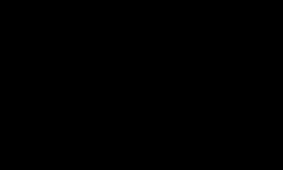
\includegraphics[width=85mm]{./imgs/im1.jpg}
\caption{\tiny{\Formular{\index{Scott, Ridley}Ridley Scott. {\slsc{Blade Runner}} (1982)}}}

\end{figure}

O pensador marxista norte"-americano \index{Jameson, Fredric}Fredric Jameson, em seu influente
\emph{Pós"-modernismo: a lógica cultural do capitalismo tardio} (1991),
chega a referir"-se ao \emph{cyberpunk} como a expressão literária
paradigmática do próprio capitalismo tardio, definindo"-o como uma
expressão das realidades das corporações multinacionais e da própria
paranoia global. Em \emph{Blade Runner}, \index{Jameson, Fredric}Jameson (2004, p.~220) enxerga
``a interfusão de multidões de pessoas em um bazar de alta"-tecnologia em
seus múltiplos pontos nodais, tudo lacrado em um interior sem exterior,
que assim intensifica o urbano anterior a ponto de tornar"-se um sistema
não mapeável do próprio capitalismo tardio''. O filósofo francês \index{Levy, Pierre@Lévy, Pierre}Pierre
Lévy (1999, p.~92) encontrou no ciberespaço de \index{Gibson, William}Gibson uma imagem
poderosa na medida em que ``torna sensível a geografia móvel da
informação, normalmente invisível''. Se \index{Jameson, Fredric}Jameson e \index{Levy, Pierre@Lévy, Pierre}Lévy atribuem tanta
importância a esse subgênero literário, é porque encontram nele, apesar
de sua superficialidade, uma valiosa proposta estética de representação
do mundo pós"-moderno, que não encontraram noutras manifestações
culturais ou artísticas.

Além de identificar essa fratura entre a experiência vivida e os
verdadeiros controladores dessa experiência, \index{Gibson, William}Gibson prevê a importância
do mundo virtual como palco de grandes embates culturais.\footnote{Utilizo aqui o termo ``virtual'' em seu sentido amplo, que diz respeito ao mundo das comunicações intermediadas pelos computadores ou ao ambiente de tecnologia digital ligado à rede. No sentido original, virtual significa algo que existe apenas como potência e possibilidade, mas que ainda não se realizou. É uma capacidade de ``vir a ser'', opondo"-se mais ao \emph{atual} do que ao \emph{real}.} No livro, o
ciberespaço é chamado de \emph{Matrix}, uma espécie de mundo paralelo,
um espaço virtual computadorizado, cujo controle é disputado por grandes
corporações e é cenário de eventuais aventuras dos personagens. Mas a
partir da popularização da internet nos anos 1990, o termo passou a
designar o ``espaço'' de interconexão de informações e dados
compartilhadas pelos computadores, confundindo"-se com a própria internet
(embora sejam coisas distintas). Mais recentemente, ganhou a atenção de
importantes pensadores contemporâneos. Na definição mais precisa de
\index{Levy, Pierre@Lévy, Pierre}Pierre Lévy (1999, p.~17), o termo especifica ``não apenas a
infraestrutura material da comunicação digital, mas também o universo
oceânico de informações que ela abriga, assim como os seres humanos que
navegam e alimentam esse universo''.

A importância do ciberespaço como um novo \emph{locus} não pode ser
subestimada, pois não se trata apenas de um sistema de troca de
informações, mas de um verdadeiro espaço cultural que, embora desterritorializado,
também permite encontros, atuações públicas e relações afetivas.
Grande parte da produção cultural, seja ela artística,
intelectual ou de entretenimento (como todo o imenso universo dos
videogames, por exemplo), acontece dentro desse universo, e foi
desenvolvida para ele, criando novas potencialidades de conexão,
mobilidade e circulação de ideias. No livro que dedica ao assunto,
intitulado justamente \emph{Cibercultura}, \index{Levy, Pierre@Lévy, Pierre}Lévy (1999, p.~113) prevê que
o ciberespaço terá um efeito tão radical sobre as comunicações quanto
teve, em seu tempo, a própria invenção da escrita. Além de canalizar um
fluxo extraordinário de informações, o ciberespaço caracteriza"-se também
pela igualmente extraordinária capacidade de armazenamento de
informações. A ``digitalização'' quase total das imagens, dos textos,
dos filmes e dos sons tornará o ciberespaço o principal suporte de
memória da humanidade.

Numa leitura otimista, o ciberespaço pode ser entendido teoricamente
como uma estrutura \emph{rizomática}, no sentido dado pelos filósofos
franceses \index{Deleuze, Gilles}Gilles Deleuze e \index{Guattari, Félix}Félix Guattari. Para eles, o
rizoma é a imagem de uma estrutura relacional onde qualquer ponto pode
se conectar com qualquer outro ponto. No rizoma não há um centro nem
hierarquias, é um modelo potencialmente infinito, onde as relações se
dão por proliferação, agregação, recomposição e conexão, e não por
alternativas, substituições e exclusões: ``um rizoma não começa nem
conclui, ele se encontra sempre no meio, entre as coisas, inter"-ser,
\emph{intermezzo}. A árvore é filiação, mas o rizoma é aliança,
unicamente aliança. A árvore impõe o verbo ``ser'', mas o rizoma tem
como tecido a conjunção `e\ldots{} e\ldots{} e\ldots{}'" (2011, p.~48).

Houve quem enxergasse nesse novo espaço sem fronteiras --- onde ``todos
falam a mesma língua'' e são ``iguais'' atrás de uma tela de computador,
onde o fluxo de informações viaja livremente, onde as coisas não se
deterioram, onde tudo parece conectar as pessoas --- um universo utópico
e ideal, quase uma religião, que iria nos salvar do mundo material e nos
libertar das próprias limitações físicas do corpo. Mas hoje percebemos
com clareza que essa promessa de integração social e comunicativa entre
os seres humanos --- uma espécie de torre de Babel informática --- não se
confirmou como anunciada. O compositor baiano \index{Gil, Gilberto}Gilberto Gil, que sempre
se mostrou atento às mudanças causadas pela tecnologia, ilustra em
algumas de suas canções esse sentimento contraditório de atração e medo
que a tecnologia desperta. Já em 1969, com a canção \emph{Cérebro
eletrônico}, o compositor fala de uma máquina que ``com seus botões de
ferro e seus olhos de vidro'' é capaz de fazer ``tudo, quase tudo''. Em
\emph{Pela internet}, lançada ao vivo na própria internet em 1996 (uma
homenagem a \emph{Pelo telefone}, de 1916, considerado o primeiro samba
gravado no Brasil), faz uma apologia da rede como espaço de comunicação
sem barreiras, com sua jangada a navegar livremente pelo ``infomar''. A
canção foi ``atualizada'' em 2018, e lançada em nova versão. Em
\emph{Pela internet 2} o compositor se mostra confuso neste novo oceano
de informações, agora sentindo"-se ``preso na rede que nem peixe
pescado''.

Se um dia a internet foi sinônimo de conectividade, de acesso, de
democracia, de ativismo, de possibilidade de união dos povos, hoje ela
significa vigilância, concentração de riqueza, monopólio da informação,
exploração do trabalho, expressão de ódio, interferência política e
alienação. As mídias sociais se tornaram um espaço paralelo onde
violentas disputas acontecem, com reflexos diretos em nossas vidas.
Dados são coletados para serem vendidos à publicidade dirigida, adolescentes são apartados do convívio social pelo excesso de estímulos virtuais, profissões precárias substituem direitos trabalhistas arduamente conquistados.

Como alerta o escritor James Bridle (2018, p.~152) em seu \emph{A nova idade das trevas}, livro em que faz uma análise sombria do futuro tecnológico, mesmo problemas gigantescos como a desigualdade social, a derrocada do estado de bem"-estar social, a ascensão de grupos de extrema"-direita, a redução das liberdades individuais e a degradação do meio"-ambiente estão relacionados com nossa incapacidade de perceber os efeitos mais amplos dessa nova realidade acelerada pelas tecnologias.

As redes sociais são um ambiente propício para a propagação de mentiras, inclusive por nós mesmos, que compartilhamos apenas os aspectos positivos de nossa experiência. Nas redes estamos sempre bonitos, em lugares interessantes, comendo bem. Ali, somos uma espécie de avatar, o personagem que gostaríamos de ser mas que, na realidade, existe apenas ali.

De forma análoga, o anonimato favorece as ``fake news'', que são distribuídas a fim de interferir em processos eleitorais, fazendo do ciberespaço o lugar da manipulação do real como estratégia de poder. Políticos pautam suas ações reagindo ao comportamento imediatista das redes. Há quem diga que o ciberespaço é hoje o principal espaço de disputa política e que, aos poucos, vai substituindo o espaço da democracia liberal, colocando em risco o próprio funcionamento das instituições democráticas, uma vez que não é submetido às regras republicanas de regulação e representatividade.

Mesmo que não seja o nosso desejo,
o fato é que grande parte de nossa vida pública, de nosso ser social e
de nossa cidadania está (e estará cada vez mais) lá dentro. Nossa
presença está agora codificada em dados que são controlados em sua maior
parte por poucas empresas, que estabelecem regras próprias de
funcionamento, sem o escrutínio do poder público, e conhecem nossos
hábitos, rotinas e trajetos, às vezes melhor do que nós mesmos. Elas são
capazes de prever nosso comportamento colocando"-se sempre um passo à
frente, adivinhando nossas preferências e oferecendo um novo
produto (seja um objeto ou um candidato à presidência da república) no
momento decisivo. Quase a totalidade da informação que circula hoje no
ciberespaço passa pelos circuitos de apenas cinco dessas empresas, todas
norte"-americanas, todas sediadas nos arredores de São Francisco. Google,
Apple, Facebook, Microsoft e Amazon detêm, juntas, um poder de controle
da informação jamais imaginado na história.

Dentro desse novo espaço público não somos tratados como cidadãos, mas
como \emph{clientes} dessas empresas. Se fornecemos nossos dados às
empresas deveríamos ter, no mínimo, o direito de saber que dados esses, onde estão armazenados, como são utilizados e quem tem acesso a eles. Deveríamos conhecer melhor a estrutura física da rede, composta de computadores, linhas telefônicas, \emph{data centers}, satélites e cabos submarinos. A internet, na verdade, é apenas a face amigável de um sistema complexo e
profundo, extremamente opaco, aparentemente neutro, que precisa ser decifrado.
Nesse novo contexto espacial, o ``direito à cidade'' proposto por \index{Lefebvre, Henri}Henri
Lefebvre talvez tenha que ser atualizado para um ``direito ao
ciberespaço''. Precisamos urgentemente desenvolver uma consciência
crítica que vá além da abordagem condescendente e tecnológica, e que
possa revelar as estruturas de poder escondidas sob o manto da
neutralidade e da hipocrisia. Até quando vamos fingir aceitar que a
verdadeira ``missão'' de uma empresa gigantesca de comunicação é ``dar
às pessoas o poder de construir a comunidade e aproximar o mundo''
(Facebook) ou ``desenvolver serviços que melhorem significativamente a
vida das pessoas'' (Google)?

\begin{figure}[!ht]

\centering
 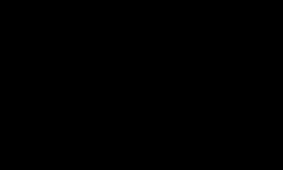
\includegraphics[width=85mm]{./imgs/im1.jpg}
\caption{\tiny{\Formular{Vista aérea do Vale do Silício}}}

\end{figure}

Mas afinal quem controla esse espaço? Seriam essas grandes empresas de
tecnologia que, além do poder econômico, agora interferem no próprio
destino das nações, influenciando sistemas eleitorais, como aconteceu
nos Estados Unidos e no Brasil?\footnote{Nos Estados Unidos, a empresa
  de análise de dados e comunicação estratégica {\slsc{Cambridge Analytica}}
  utilizou --- provavelmente de forma ilegal --- dados pessoais
  armazenados no Facebook para interferir decisivamente na eleição
  norte"-americana que culminou na vitória de \index{Trump, Donald}Donald Trump. No Brasil, o
  vencedor das eleições presidenciais de 2018 contou com uma vasta
  distribuição de notícias falsas via aplicativo Whatsapp (que pertence
  ao Facebook) nos dias anteriores à votação.} Ou será que a rede se
tornou ingovernável, onde nenhum grupo político, econômico ou
intelectual define o curso dos eventos e é capaz de controlar o
cruzamento de todos os fluxos de saber ali depositados?

A rede nos levou a uma ``algoritmização'' da vida, pela qual as decisões
humanas se tornam interpretações de cálculos automáticos.\footnote{Ver ``The Secret Rules of Modern Living Algorithms'', documentário da \scalebox{.8}{BBC} produzido por \index{Sautoy, Marcus Du}Marcus Du Sautoy.} Os
investimentos, as estratégias de ação, o destino dos recursos sociais e
as decisões políticas são cada vez mais determinados pelo resultado de
equações matemáticas que, por sua vez, são baseadas na coleta de dados
de milhões de pessoas. Os algoritmos analisam esses dados e são capazes de prever nossas necessidades com bastante precisão. Além disso, os algoritmos se aprimoram com o próprio uso, conforme fornecemos mais dados a ele, gerando o chamado \emph{big data}, uma quantidade tão vasta de informação que apenas sistemas sofisticadíssimos têm a capacidade de decrifrar. Isso mobiliza tanto a ciência quanto as grandes corporações, cada vez mais voltadas para a decifração do \emph{big data}, e seu potencial de eficiência.\footnote{No entanto, nunca devemos perder de vista que a eficiência, ao contrário do que o mundo capitalista refém do crescimento econômico quer nos fazer acreditar, não é um valor moral. Basta pensarmos nas máquinas de guerra e nos instrumentos de tortura. Há um conto de Kafka que ilustra bem essa questão. Em {\slsc{Na colônia penal}}, um agente da justiça descreve uma complexa máquina de punição que inscreve a sentença diretamente na pele do condenado, com agulhas perfurando lentamente a pele. Ver \scalebox{.8}{KAFKA}, Franz. {\slsc{Na colônia penal}}. Rio de Janeiro: Paz e Terra, 1996.}

As decisões que estão determinando nosso futuro
estão cada vez mais submetidas não à vontade humana com sua ousadia e
poder de imaginação, mas ao resultado de uma média ponderada coletada
por máquinas ``com seus botões de ferro e seus olhos de vidro'', capazes
de prever com alto grau de acerto os comportamentos humanos. Com isso,
o poder, aparentemente invisível, passa a residir na programação da
máquina e de seus algoritmos.

No limite, com as decisões tomadas cada vez mais por máquinas
``inteligentes'', os humanos se tornarão obsoletos e marginais,
exatamente como numa novela \emph{cyberpunk}, sem poder de ação. A imagem dessa
nova condição humana se assemelha de forma perturbadora com a descrição
de \index{Gibson, William}Gibson acerca do ciberespaço distópico. Para o filósofo italiano
\index{Berardi, Franco}Franco Berardi (2009, p.~126), a humanidade é ``reduzida a um `twist
finger', a um dedo que se agita, a um corpo paralisado e a uma bomba de
informação supersaturada que navega em canais e realiza escolhas no
interior de limites estritamente programados''.

\chapter{A chegada do fututo}

Na modernidade o futuro era visto como fonte de esperança. O futuro
traria o retorno do investimento do presente, num mundo que acreditava
cegamente no crescimento econômico, nos avanços da ciência, na
acumulação do conhecimento e na prosperidade da civilização. Futuro e
progresso eram a mesma coisa.

Mas a história do futuro nos mostra que nem sempre foi assim, tendo
atravessado variações de percepção e de imaginação através da história,
nos explica \index{Berardi, Franco}Berardi (2019, p.~93). Nas civilizações tradicionais, diz
ele, a visão do futuro pode ser maldita, destino trágico dos visionários
e dos profetas que ousam tentar ver o que só aos deuses é dado ver. Já
no mundo cristão, a mente se dirige ao passado, à origem divina do
mundo, onde se encontra o criador e a luz. O futuro é queda e escuridão,
que pode nos levar ao juízo final.

Neste início do século \versal{XXI}, o futuro parece sombrio novamente. \index{Berardi, Franco}Berardi
identifica esse sentimento numa geração que cresceu em meio a um
individualismo desenfreado, formada por pessoas que confiaram nas
promessas do egoísmo neoliberal e de sucesso individual e se descobriram
perdedoras, restando a elas ressentimento e ódio. Não à toa, temos visto
nos últimos anos uma retomada das grandes narrativas distópicas do
século \versal{XX}. Desde a paranoia nuclear dos anos 1970, não se viam tantas
obras empenhadas em especular sobre o fim do mundo. A ascensão de novos
regimes autoritários de direita, o crescimento vertiginoso e
descontrolado das cidades, as condições precárias do trabalho, os abusos
das empresas de tecnologia e a real ameaça de uma catástrofe ecológica
criaram condições para o renascimento dessa estética sombria.

Essa linhagem distópica, que remonta à literatura de fantasia e aventura
no século \versal{XIX}, tem um marco visual importante justamente com
\emph{Metropolis} (1927), de \index{Lang, Fritz}Fritz Lang, que retrata um mundo futurista
e hiperindustrializado, onde a força de trabalho operária é explorada
sem clemência por magnatas e homens de negócio. É também dessa época um sombrio conto de \index{Lovecraft, H. P.}H. P. Lovecraft, \emph{O chamado de Cthulhu} (1926), em que o narrador alerta para os problemas decorrentes do excesso de informação, antecipando o perigo da internet como depositária única da informação e do conhecimento. Da mesmo forma, é difícil deixar de vislumbrar nesse parágrafo uma premonição do estado de cegueira que vemos nesse início do século \versal{XXI}, pleno de discursos simplificados que, por sua vez, têm permitido a ascensão de regimes autoritários, apologéticos da ignorância:

\begin{quote}
A coisa mais misericordiosa do mundo, acho eu, é a incapacidade da mente humana correlacionar tudo que ela contém. Vivemos numa plácida ilha de ignorância em meio a mares tenebrosos de infinidade, e não estávamos destinados a chegar longe. As ciências, cada uma puxando para seu próprio lado, nos causaram poucos danos até agora, mas algum dia a junção das peças do conhecimento disperso descortinará visões tão terríveis da realidade e de nossa pavorosa posição dentro dela que só nos restará enlouquecer com a revelação ou fugir da iluminação mortal para a paz e a segurança de uma nova idade das trevas (\versal{LOVECRAFT}, 2000, p.~103).\index{Lovecraft, H. P.}
\end{quote}

Seguiram"-se as previsões
de um mundo totalitário, regido pela ordem do Estado como em
\emph{Admirável mundo novo} (1932), de \index{Huxley, Aldous}Aldous Huxley, e \emph{1984} (1948), de \index{Orwell, George}George Orwell, com seu
``Grande Irmão'' onisciente e invasivo, prefigurando o regime de
vigilância paranoica que vivemos nas grandes metrópoles do século \versal{XXI}. O
mundo também foi ameaçado por monstros gigantes como \emph{Godzilla} (1954),
resultado de um acidente nuclear num país ainda traumatizado pelos
efeitos da bomba atômica. Já as ficções cinematográficas dos anos 1980
como \emph{O exterminador do futuro} (1984) e \emph{Robocop} (1987)
apostavam na revolução tecnológica do corpo.

Lançado no auge do movimento punk, \emph{Mad Max} (1979) se passa num
futuro pós"-apocalíptico e decadente onde os personagens lutam pela
própria sobrevivência em meio à escassez de recursos. Ambientado no
deserto da Austrália, numa terra sem lei nem governo, a gasolina se
torna a principal moeda de troca e é violentamente disputada. O filme é
uma espécie de encontro do \emph{road movie} e do \emph{western} com o
\emph{cyberpunk}, prefigurando seus personagens marginais e solitários,
dependentes das máquinas e abandonados à própria sorte. Nos anos 1990,
filmes como \emph{Armageddon} (1998) \emph{Impacto profundo}
(1998) e \emph{Independence Day} (1996) acreditavam que a ameaça do fim
do mundo viria de fora, na forma de alienígenas assassinos ou de corpos
celestes em rota de colisão com a Terra. Depois da ficção tornada
realidade com os ataques de 11 de setembro de 2001, evento que esgota o
``cinema"-catástrofe'', filmes como \emph{Fim dos tempos}, de \index{Shyamalan, M. Night}M. Night
Shyamalan (2008) e \emph{Melancolia}, de \index{Trier, Lars von}Lars von Trier (2011) vão em
busca de respostas metafísicas para o fim do mundo.

Com exceção de \emph{Metropolis}, que pode ser entendido como uma
extensão sombria da revolução industrial, em quase todas essas
narrativas o fim do mundo dependia de um rompimento da ``ordem natural''
da história, seja com uma guerra, um monstro ou uma
catástrofe. Agora isso não é mais necessário.

\begin{figure}[!ht]

\centering
 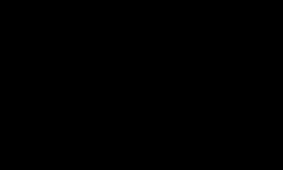
\includegraphics[width=85mm]{./imgs/im1.jpg}
\caption{\tiny{\Formular{\index{Lang, Fritz}Fritz Lang. {\slsc{Metropolis}} (1927)}}}

\end{figure}

Das muitas obras e subgêneros de ficção científica produzidas no século
\versal{XX} que procuraram prever um futuro para a humanidade o \emph{cyberpunk}
parece ser o que mais próximo chegou da realidade que experimentamos no
século \versal{XXI}. É verdade que ainda não há carros voadores nem clones
humanos superinteligentes mas, à sua maneira, o \emph{cyberpunk} acerta
na representação estetizada desse mundo em que vivemos, onde o homem não
tem acesso às verdadeiras instâncias do poder e cujo funcionamento não
entende perfeitamente.\footnote{Esta é também a condição ``kafkiana''
  por excelência. Penso aqui na definição de \index{Borges, Jorge Luis}Jorge Luis Borges: ``duas
  ideias --- ou melhor --- duas obsessões regem a obra de \index{Kafka, Franz}Franz Kafka. A
  subordinação é a primeira das duas; o infinito, a segunda. Em quase
  todas suas ficções há hierarquias e essas hirerarquias são infinitas''
  (\scalebox{.8}{BORGES}, 2007, v. \scalebox{.8}{IV}, p.~117). Ver página \scalebox{.8}{XXXX} (o ``comando'' de
  Kafka).} Acerta também na antecipação daquilo que vem sendo chamado de
``fim do futuro'' --- esse sentimento de impotência diante do fracasso
das utopias, essa resignação diante de nossa própria incapacidade de
transformar a realidade, condenada a um imediatismo paranoico. O
\emph{cyberpunk} é povoado por esses personagens sem esperança nem
perspectiva, que vivem num eterno presente imersivo, sem saber se amanhã
estarão vivos.

A utopia da rede virtual, este espaço desterritorializado, onde se
cruzariam as trajetórias de agentes libertários, talvez tenha sido a
última grande utopia do século \versal{XX}. Em seu estado inicial, o ciberespaço
foi um espaço promissor da imaginação política e social, abrindo
possibilidades impensáveis até então. Mas a ideia de que a democracia finalmente
encontraria no território virtual da rede seu ambiente ideal
provou"-se uma grande ilusão, pois as mesmas disputas que travamos na
realidade do mundo territorial, dominado por interesses econômicos,
foram transpostas à rede.

\index{Berardi, Franco}Franco Berardi (2019, p.~103) sustenta que o grande salto tecnológico do
capitalismo foi possível pela convergência de dois fatores: a
desregulamentação da economia e o advento da internet.\footnote{Popularizada
  nos anos 1990, a World Wide Web facilitou e organizou de forma inédita
  a circulação de dados que até então era restrita a sistemas
  sofisticados. Com a ``interface'' amigável de seus ``navegadores'',
  foi a porta de acesso a um novo espaço informacional que nunca mais
  parou de crescer. A ``invenção'' desse sistema é creditada ao
  britânico \index{Berners-Lee, Tim}Tim Berners"-Lee. Por ocasião dos 30 anos do invento, o
  cientista divulgou uma carta onde mostra preocupação com o possível
  ``futuro disfuncional'' da intenet. Ver ``\index{Berners-Lee, Tim}Sir Tim Berners"-Lee spoke to
  the \scalebox{.8}{BBC}'s Rory Cellan"-Jones''. \scalebox{.8}{BBC}, 2019.} Há uma relação íntima e
conflituosa entre a rede como espaço de compartilhamento social e o
sistema integrado do neocapital que, juntos, transformaram a produção e
a comunicação global. É neste contexto de abertura neoliberal que,
segundo \index{Berardi, Franco}Berardi, surge a cibercultura. A utopia de liberdade
ciberespacial é o produto do encontro da desregulamentação econômica
promovida pelo neoliberalismo com o espírito de liberdade criativa e
cultura libertária, cuja matriz anárquica e psicodélica remonta à
geração beatnik da costa oeste americana nos anos 1960.

No entanto, a rebeldia anárquica que pregava a quebra das regras de
comportamento social é completamente diferente da ausência de regras
necessárias para regular a economia. Se a utopia da conexão virtual
propunha um mundo de igualdade e justiça, onde ``todos somos iguais
perante a rede'', o objetivo da desregulamentação neoliberal é a
destruição do estado social, entendido como empecilho que trava o
mercado ``capaz de regular a si mesmo''. No entanto, é justamente esse
estado social o responsável pela contenção das injustiças e pela
distribuição da riqueza.

Não poderia dar certo. A utopia da rede foi substituída agora por um
mundo de desesperança e resignação, uma distopia presentificada onde o
ser humano sucumbe exausto aos automatismos e ditames do neoliberalismo,
como se viajasse numa aeronave ligada em piloto automático e cujo
destino não pode ser mudado. Não há no horizonte da humanidade nenhum
vislumbre de mudança radical, nenhum grande projeto coletivo, nenhuma
revolução. Nada para além do projeto pós"-humano californiano de corporações e \emph{startups}, crente no poder da tecnologia como salvadora do indivíduo e do mundo, mas no fundo excludente e profundamente vinculado ao capital. As distopias realizadas agora (penso da série televisiva
\emph{Black Mirror}) enxergam um futuro sombrio demasiadamente próximo e
palpável, a um passo de se realizar.

O fato é que deveríamos ter levado William Gibson a sério. Havia uma dimensão crítica em sua obra para além da aparente superficialidade de uma literatura marginal. A distopia dos anos 2010, produto direto do fracasso, nos anos 2000, da
utopia cibercultural surgida nos anos 1990, foi percebida e antecipada
nos anos 1980 por autores como ele. O \emph{cyberpunk} já tinha percebido que não há acordo
entre um jovem de espírito anárquico e libertário, de um lado, e os
agentes do capital, do outro. Não há diálogo possível entre o punk
urbano da periferia de Londres e o yuppie neoconservador que trabalha na
bolsa de Nova York, dois personagens emblemáticos dessa época. É desse
atrito que nasce o \emph{cyberpunk}, que transformou essa índole
anárquica em violência contra o próprio sistema tecnocrático, seja ele
representado pelo Estado ou pelas grandes corporações.

No \emph{cyberpunk} não há mais espaço para os heróis que podem salvar o mundo,
como em muitas histórias de ficção científica. As cidades são tomadas
por personagens individualistas, preocupados em salvarem a si mesmos, sem
tempo para pensar na salvação do planeta. A única esperança está
depositada na figura emblemática e solitária do hacker, misto de herói e
bandido, que sabe que a única salvação está em corromper o sistema por
dentro, decifrando seu código.

\chapter{Grades brilhantes de lógica sobre vácuo sem cor}

Há uma enorme dificuldade para compreendermos o mecanismo e
funcionamento do ciberespaço. Ele nos chega através de uma tela
luminosa, atraente e colorida, mas não conseguimos enxergar suas peças e
suas entranhas.\footnote{\index{Gil, Gilberto}Gilberto Gil fala de nossa dificuldade para
  encarar essa nova dimensão espacial ``quando nos postamos diante dela
  com a postura que tínhamos com relação ao mundo das coisas sólidas''.
  Ver \scalebox{.8}{LICHOTE}, Leonardo. ``Tempo rei''. {\slsc{O Globo}}. Rio de Janeiro, 26
  nov. 2007, p.~3.} Sua face visível nos promete ``acesso'' às
informações distantes ao mesmo tempo em que esconde sua própria
estrutura, espalhada pelo planeta e controlada por grandes empresas. Daí
nossa imensa dificuldade em \emph{mapearmos} satisfatoriamente esse
espaço imaterial.

Se no início entendíamos positivamente a estrutura do ciberespaço como
um rizoma deleuziano, hoje talvez seja melhor entendê"-lo
negativamente como um labirinto, esse edifício que se define pela
própria ideia de desorientação, dentro do qual nunca sabemos exatamente
onde estamos.\footnote{Mesmo o ciberespaço, com toda sua virtualidade,
  possui uma ``arquitetura'' própria. O termo ``arquitetura de rede''
  refere"-se a ``um edifício funcional composto de equipamentos de
  transmissão, de softwares e protocolos de comunicação e de uma
  infra"-estrutura filiar ou radioelétrica que permite a transmissão dos
  dados entre os diversos componentes''. Ver: \textless{}{\slsc{https://br.ccm.net/}}\textgreater{}.} Ainda
mais sufocante do que o labirinto arquitetônico, que ainda possibilita a
existência do mapa, o ciberespaço é um labirinto ``imapeável'' e
caótico, em expansão contínua, isolando cada vez mais o indivíduo em seu
centro, e impedindo por completo seu entendimento estrutural.\footnote{Ver
  página \scalebox{.8}{XXXXXX}.} O território das possibilidades infinitas que o
ciberespaço representa deixa de ser uma utopia libertadora para se
tornar sinônimo de impossibilidade, de fadiga e de desespero. A aparente ausência
de barreiras é apenas uma ilusão que não impede a configuração
essencial da situação labiríntica, com todo seu potencial encantador e
ardiloso. Um labirinto não mais como o edifício de \index{Dedalo@Dédalo}Dédalo, mas como um
deserto borgiano.\footnote{Ver página \pageref{borges}.}

Uma das primeiras representações do ciberespaço pode ser encontrada no
filme \emph{Tron} (1982), produzido pela Disney e dirigido por \index{Lisberger, Steven}Steven
Lisberger (e lançado no mesmo ano de \emph{Blade Runner}). O enredo
trata de uma disputa entre programadores que desenvolvem softwares para
videogames. O personagem principal busca uma forma de resolver a disputa
invadindo literalmente o sistema, onde é submetido a uma série de
desafios, tendo que participar de jogos mortais contra os adversários.

\begin{figure}[!ht]

\centering
 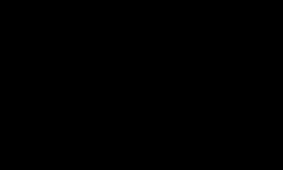
\includegraphics[width=85mm]{./imgs/im1.jpg}
\caption{\tiny{\Formular{\index{Lisberger, Steven}Steven Lisberger. {\slsc{Tron}} (1982)}}}

\end{figure}

\emph{Tron} retrata o ciberespaço como um lugar onde se pode entrar, mas
de onde é difícil sair, justamente como num labirinto. Ali dentro
pode"-se ter uma espécie de vida paralela --- uma concepção que antecipa
as interações virtuais em rede do mundo contemporâneo, sobretudo os
jogos eletrônicos e as redes sociais. O filme não foi muito bem
compreendido na época (a trama era extremamente confusa e poucas pessoas
possuíam computadores em casa), mas foi pioneiro na busca de uma
estética própria para o universo dos computadores.\footnote{Depois
  aperfeiçoada no filme {\slsc{Matrix}} (1999), das irmãs \index{Wachowski, Lana e Lilly}Wachowski.} O
ciberespaço de \emph{Tron} é luminoso, colorido e labiríntico, como o
universo dos videogames Atari dos anos 1980. As superfícies são lisas,
inorgânicas, desprovidas de texturas e de qualquer coisa que lembre
formas da natureza. Há raios de luzes fluorescentes e sons eletrônicos,
sugerindo uma trama em rede de comunicação imediata. É um universo
alucinante regido pela velocidade. A batalha principal se dá numa imensa
superfície quadriculada, como num tabuleiro infinito onde motos
futuristas deslizam em altíssima velocidade, lembrando as ``grades
brilhantes de lógica se desdobrando sobre aquele vácuo sem cor'', como
na \emph{Matrix} no livro de \index{Gibson, William}Gibson (2016, p.~25).

Analisado de um ponto de vista cultural, o ciberespaço seria, portanto, uma
espécie de metáfora precária de um problema que se estende por toda
parte. Os conflitos sociais, políticos e econômicos de nossa época
também são caracterizados por essa ``desterritorialização'' do espaço,
onde uma decisão tomada num ponto do planeta afeta imediatamente a vida
de cidadãos situados a milhares de quilômetros dali, sem nenhum contato
entre as partes. Essa distância já é tão grande que chegou ao ponto de
ruptura --- já não sabemos quem de fato toma as decisões que determinam o
funcionamento da sociedade como um todo. Apesar das promessas de
democracia e liberdade, o mundo do neocapitalismo globalizado não se
caracteriza exatamente pela transparência, mas, ao contrário, por um
sistema que nega acesso ao entendimento de seu mecanismo. Assim, a
própria dificuldade em representar o ciberespaço se assemelha com a
dificuldade de representar o complexo sistema do capitalismo
multinacional em que vivemos. Apesar da metáfora sedutora de um universo
tecnológico interconectado, o complexo mundo em que vivemos
caracteriza"-se, entre outros aspectos, justamente pela maneira esquiva
com que escapa a qualquer proposta de representação.\footnote{\index{Wisnik, Guilherme}Guilherme
  Wisnik propõe a imagem de um ``nevoeiro'' como metáfora desse mundo
  regido pela opacidade e pela falta de clareza. Ver \scalebox{.8}{WISNIK}, Guilherme.
  {\slsc{Dentro do nevoeiro: arquitetura, arte e tecnologia contemporâneas}}. São
  Paulo: Ubu, 2018.}

Se, por um lado, o conceito de pós"-modernismo parece já antiquado do
ponto de vista da análise cultural mais ampla, ele, por outro lado,
mantém sua atualidade quando analisamos a problemática de representação
do espaço.\footnote{Ver \index{Foster, Hal}\scalebox{.8}{FOSTER}, Hal et al. {\slsc{Art since 1900:
  Modernism, Antimodernism, Postmodernism}}. Londres: Thames \& Hudson,
  2016, p.~689.} Na verdade, não só o problema estético e
representacional a respeito dessa dificuldade permanece bastante atual
como, de certa forma, a aceleração exponencial das transformações do
mundo parece apenas radicalizar a percepção de que estamos cada vez mais
distantes de uma imagem mental que dê conta das complexidades desse
espaço.

Uma das principais características estéticas do pós"-modernismo é
justamente sua superficialidade --- uma ``falta de profundidade'' em que as
representações frequentemente são mais importantes do que as coisas
representadas e onde a realidade é substituída por pastiches e
simulacros. Esta
superficialidade é justamente o mérito e o limite de um gênero literário
marginal como o \emph{cyberpunk}. Se, por um lado, ele é capaz de
representar, com sua superficialidade, a superficialidade desse mundo,
por outro não dá conta (nem pretende) das verdadeiras complexidades
escondidas por detrás de toda essa superficialidade. Desta forma,
encontrar uma forma eficiente de representação estética do funcionamento
desses mecanismos deve ser um projeto urgente para compreendermos melhor
o complexo ambiente em que vivemos. Mais ainda, seria o pré"-requisito
incontornável para atuarmos sobre esse mundo a fim de transformá"-lo.

\chapter{Um salto no escuro}

A humanidade passou por um importante ciclo de invenções no século \versal{XIX}
que ``encurtou'' as noções de espaço e de tempo. O telefone, a
locomotiva a vapor e a fotografia, por exemplo, aproximaram coisas que
estavam distantes, e simbolizaram uma época associada ao progresso
tecnológico e social. Agora, estamos passando por um novo ciclo de
aceleração, impulsionado por tecnologias que num passado recente eram
encontradas apenas nos filmes de ficção científica. Estamos num momento
de redefinição da própria experiência perceptiva causada pelos novos
ritmos e velocidades que nos são impostos pelas máquinas e pelas novas
formas de consumo.

No entanto, é preciso salientar que a aceleração não é algo exclusivo de
determinados momentos históricos, mas é o próprio fundamento da
sociedade em que vivemos. As sociedades modernas são essencialmente
``aceleracionistas'', ou seja, são fundadas na ideia de acúmulo,
crescimento e progresso intermináveis. Podemos entender essa
característica à luz da distinção proposta pelo antropólogo francês
\index{Levi-Strauss, Claude@Lévi-Strauss, Claude}Claude Lévi"-Strauss acerca das sociedades ``frias'' e sociedades
``quentes''. Se as primeiras são aquelas que privilegiam a estabilidade
e resistem às mudanças, percebidas como desagregação e desordem, as
sociedades ``quentes'' (como a nossa) se caracterizam pela acumulação,
valorizando o progresso e a transformação tecnológica.

O capitalismo neoliberal confunde a ideia de progresso e desenvolvimento
com o crescimento econômico permanente e vai fazer de tudo para que esse
crescimento seja o maior possível, pouco importando as consequências
sociais, políticas ou ecológicas. Essa lógica insustentável, onde a
própria ideia de crise é entendida como falta de crescimento, é a
própria ideologia do modelo neoliberal (mesmo que o neoliberalismo
recuse a aceitar que possua qualquer ideologia, como se fosse o produto
natural e neutro da democracia).

Portanto, o que é característico de nossa época não é a aceleração em
si, mas o crescimento exponencial de sua velocidade, que agora
ultrapassa nossa capacidade de acompanhamento, criando uma lacuna --- um
``espaço'' --- entre nós e o mundo. No capitalismo, aceleração da
velocidade e crescimento econômico constante são duas faces de uma mesma
moeda, necessárias para o próprio funcionamento do sistema. A meta é
sempre a maior quantidade de produção no menor espaço de tempo.
Portanto, o incremento da produtividade é alcançado pelo aumento da
aceleração. E a aceleração se faz ou pelo aumento da carga de trabalho,
ou pelo uso da tecnologia.

Por mais que a tecnologia represente progresso, ainda não foi possível
transformar essa nova condição numa vantagem crítica; pelo contrário,
ainda estamos numa condição passiva ou, na melhor das hipóteses,
``reativa'', a reboque dos inventos e novidades que nos pegam de
surpresa a todo momento e dos lançamentos dos dispositivos tecnológicos
``revolucionários'' (que confundimos com a própria noção de tecnologia).
Sempre, portanto, um passo atrás do sistema de produção e consumo,
incapazes de pautar as discussões que problematizam esse mesmo sistema.
Na verdade, há muito tempo que os produtos nem são mais concebidos para
suprirem uma necessidade humana, mas são inventados para criarem uma
necessidade que nunca havia existido. Essa capacidade de antecipação da
demanda é um dos atributos mais desejados no mundo nos negócios, muitas
vezes propagado como sinônimo de ``inovação''.\footnote{A figura mais
  emblemática desse modo de produção é sem dúvida o fundador e \scalebox{.8}{CEO} da
  Apple, \index{Jobs, Steve}Steve Jobs (1955-2011). Desde os anos 1970, Jobs desenvolveu
  (juntamente com o engenheiro \index{Wozniak, Steve}Steve Wozniak) uma série de computadores
  pessoais, culminando com o {\slsc{Macintosh}} (1984), o primeiro
  computador de consumo com interface gráfica. A partir dos anos 1990
  lançou uma série de produtos ``inovadores'' como o {\slsc{Imac}} (1998),
  o {\slsc{Ipod}} (2001), o {\slsc{Iphone}} (2007) e o {\slsc{Ipad}} (2010),
  levando a Apple para o topo das empresas mais valiosas do mundo.}

Portanto, o que poderíamos chamar de progresso é, muitas vezes, apenas
aceleração, fazendo chegar a nós, com mais velocidade do que somos
capazes de absorver, aquilo que não precisamos. É um sistema que nos
deixa como reféns da velocidade, pois estamos sempre atrás (tanto no
sentido de ``atrasados'' quanto de ``em busca'') da próxima novidade,
que nunca alcançaremos, como no paradoxo de \index{Zenão de Eleia}Zenão.\footnote{O paradoxo,
  atribuído ao filósofo pré"-socrático \index{Zenão de Eleia}Zenão de Eleia, é contado na forma
  de uma corrida entre Aquiles e a tartaruga. O herói, mais veloz, larga
  atrás da tartaruga e pretende ultrapassá"-la. Mas não consegue nunca
  alcançá"-la pois, quando chega no ponto onde ela estava, a tartaruga já
  avançara um pouco e se encontra mais adiante (A nunca alcançará B,
  porque B já estará em C). E assim o processo se repete infinitamente.
  \index{Borges, Jorge Luis}Jorge Luis Borges enxerga nessa angústia a essência da condição
  kafkiana. Ver \scalebox{.8}{BORGES}, Jorge Luis. ``\index{Kafka, Franz}Kafka y sus precursores'', in
  {\slsc{Obras completas \scalebox{.8}{II}: 1952-1972}}. Buenos Aires: Emecé, 2007, p.~107.} Assim como os aparelhos e os softwares, nós mesmos precisamos
nos ``atualizar'' a todo momento, por isso temos a sensação de estar
sempre atrasados, devendo algo, com a sensação de culpa. Esse estado é a
receita da tensão, da ansiedade, da frustração, da depressão, da
paralisia do desejo erótico e de uma série de patologias contemporâneas.
Há um esgotamento físico e mental diante das metas inatingíveis
colocadas tanto pela necessidade de consumo quanto pelas pressões de uma
sociedade baseada no desempenho produtivo.

A tecnologia reduz o tempo do trabalho, mas o neocapital se apropria
novamente do tempo liberado, identificando nele um desperdício
improdutivo. O filósofo sul"-coreano \index{Han, Byung-Chul}Byung"-Chul Han (2015, p.~33) enxerga
nessa condição de ``hiperatenção'' permanente, sem momentos de repouso,
um estado selvagem, próprio dos animais que precisam exercer diversas
atividades simultaneamente para garantir a própria sobrevivência.
Impedindo, portanto, o momento da atenção profunda e contemplativa,
produtor da filosofia, da imaginação e da cultura civilizatória. Nesse estado de
``permanente provisoriedade'' a ideia de planejamento dá lugar a uma
incessante gestão de risco que, pela própria natureza emergencial, nos
impede de agir sobre nossa realidade de forma propositiva, como se
estivéssemos apagando incêndios sucessivos. E tudo o que os agentes do
neocapital desejam é que os indivíduos permaneçam ocupados, calados,
produzindo e consumindo. Pois enquanto estamos superocupados, as
relações de poder permanecem as mesmas --- uma fórmula perversa e
absolutamente contemporânea que o ensaísta \index{Crary, Jonathan}Jonathan Crary (2016, p.~44)
em seu \emph{24/7: capitalismo tardio e os fins do sono} chamou de
``manutenção calculada de um estado de transição contínuo''.

Se o espaço virtual é potencialmente ilimitado, e continua se
expandindo, a capacidade humana de apreensão desse espaço, com nossos
limites orgânicos, emocionais e culturais, não se alterou muito. O corpo
humano ainda obedece ao limite da experiência das coisas vividas e da
capacidade de nosso cérebro para processar essa avalanche de informação
e estímulos que o ciberespaço despeja.

Esses limites não se aplicam à velocidade do processamento de dados de
informática. Em 1975 o engenheiro norte"-americano \index{Moore, Gordon E.}Gordon E. Moore previu
que o número de transistores dos chips --- portanto a capacidade de
processamento de dados --- dobraria a cada dois anos. Esta previsão, que
se verificou bastante acurada, acabou ganhando o nome de Lei de Moore que, representada como uma linha diagonal ascendente, mimetiza bem a aceleração da experiência que percebemos nessas últimas décadas. É
impossível para o cérebro humano acompanhar essa expansão da capacidade de
processamento e armazenamento de informações, pois estamos presos ao
ritmo lento da matéria orgânica, e sujeitos ao cansaço, aos desejos e ao
sofrimento do corpo. Mesmo aumentando nosso tempo de atenção, trabalhando mais ou
fazendo uso de drogas, nosso ritmo de aceleração jamais chegará à
equação da \index{Moore, Gordon E.}Lei de Moore.

Em algum momento no final do século passado deu"-se uma grande mudança
cultural, decorrente de profundas transformações político"-econômicas. Ao
analisarmos as teorias históricas, culturais e sociológicas produzidas
nos anos 1980 e 1990, percebemos que alguns pensadores identificaram no
início dos anos 1970 o momento crucial dessa mudança --- que vai
acarretar numa nova relação do homem com seu entorno espacial. O
geógrafo inglês \index{Harvey, David}David Harvey, por exemplo, no influente \emph{Condição
pós"-moderna} (1989) identifica esse momento por volta de 1972, com a
mudança do paradigma econômico: do regime fordista de produção para um
sistema de acumulação flexível, seguido por uma impressionante revolução
tecnológica. Um pouco antes, em 1971, o presidente norte"-americano
\index{Nixon, Richard}Richard Nixon havia desvinculado o dólar do ouro, eliminando a regra da
conversibilidade estabelecida nos acordos de Bretton Woods em 1944,
abrindo caminho para os diversos modos de especulação financeira
baseados na desmaterialização do dinheiro. É também nessa época que o
historiador \index{Hobsbawm, Eric}Eric Hobsbawm (2003, p.~402) situa a passagem da ``era de ouro'' do
capitalismo para o que chamou de ``era do desmoronamento'',
caracterizada por instabilidades e crises causadas sobretudo pela
``transnacionalidade'' da nova economia mundial.

O que afinal se percebeu foi uma transformação no interior da própria
estrutura do capitalismo, acompanhada por uma inovação tecnológica que
deu ainda mais impulso a essa mudança. Fatores como o domínio das
empresas transnacionais sobre o Estado, a descentralização e a
``financeirização'' da economia, a primazia do setor de serviços sobre a
produção industrial, a facilidade e a velocidade das transferências de
capital especulativo, as novas formas de transporte de mercadorias e a
fuga da produção para regiões da Ásia, impactaram de forma dramática
todos os países do mundo, ``globalizando'' tanto a economia mundial
quanto as injustiças e desigualdades decorrentes dessa mesma
globalização.

Acrescente"-se a isso o próprio crescimento da população mundial, que
praticamente dobrou nesse mesmo período. Se éramos 3,9 bilhões em 1972, agora somos
7,7 bilhões de habitantes, segundo a \versal{ONU}.\footnote{United Nations,
  Department of Economic and Social Affairs, Population Division (2019).
  {\slsc{World Population Prospects 2019, Online Edition}}.} Um cálculo
matemático da quantia de experiência humana vivida ao longo da história
mostra que 15\% de toda essa experiência pertencem a pessoas que estão
vivas nesse exato momento.\footnote{Ver \scalebox{.8}{RAY}, Georgia. {\slsc{The funnel
  of human experience.}} 2018.}

\begin{figure}[!ht]

\centering
 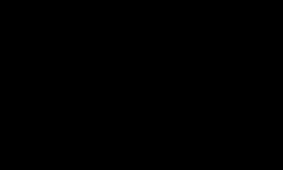
\includegraphics[width=85mm]{./imgs/im1.jpg}
\caption{\tiny{\Formular{Michael Wolf. {\slsc{Architecture of density \#116}}, Hong Kong (2009)}}}

\end{figure}

\begin{figure}[!ht]

\centering
 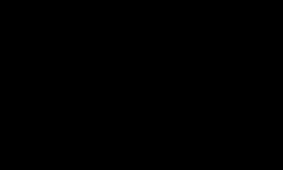
\includegraphics[width=85mm]{./imgs/im1.jpg}
\caption{\tiny{\Formular{Edward Burtynsky. {\slsc{Manufacturing \#2}}, Mudança de turno, Fábrica Yuyuan Shoe, Gaobu, China (2004)}}}

\end{figure}

O crescimento vertiginoso e descontrolado das cidades dos países em
desenvolvimento é o retrato urbano dessas transformações sociais, com
toda sua atração sedutora e toda sua precariedade. A facilidade do
deslocamento humano por via aérea e o turismo de massa diminuíram as
distâncias entre os povos, permitindo um contato entre as pessoas
inimaginável no início do século \versal{XX}. No campo das mídias e das
comunicações, a expansão das tecnologias digitais de informação, a
``imagificação'' do cotidiano e a substituição da imprensa pela
circulação virtual de dados e informações ``desmaterializaram'' o
contato entre as pessoas, transformando a comunicação num fenômeno
instantâneo e ubíquo. Todos esses fatores combinados aceleraram
exponencialmente a experiência humana de uma forma jamais vista.

Pensadores como Fredric \index{Jameson, Fredric}Jameson, \index{Virilio, Paul}Paul Virilio e \index{Bauman, Zygmunt}Zygmunt Bauman
detectaram nesse momento um ponto de ruptura sem precedente na história
da humanidade. Eles perceberam que a aceleração da experiência e o
crescimento das instituições que regulam nossa vida colocaram as
estruturas de poder para além da nossa capacidade de apreendê"-las de
forma sensível, gerando o que podemos chamar de ``crise da
experiência''. Perceberam o surgimento de uma ``lacuna entre a percepção
fenomenológica e a realidade que transcende todo pensamento ou
experiência individuais'' (\versal{JAMESON}, 2000, p.~411), um ``desequilíbrio
perigoso entre o sensível e o inteligível'' (\versal{VIRILIO}, 1993, p.~23), uma
``disjunção alarmante entre o corpo e o ambiente construído'' (\versal{JAMESON},
2000, p.~70), um ``desequilíbrio entre a informação direta de nossos
sentidos e a informação mediatizada das tecnologias avançadas''
(\versal{VIRILIO}, 1993, p.~40), uma ``nova assimetria entre a natureza
extraterritorial do poder e a contínua territorialidade da `vida como um
todo'" (\versal{BAUMAN}, 1999, p.~16), uma ``contradição crescente entre a
experiência do vivido e a estrutura'' (\versal{JAMESON}, 2000, p.~406). Essa nova
condição na qual ``a verdade da experiência não mais coincide com o lugar
onde ela se dá'' (\versal{JAMESON}, 2000, p.~406) vai transformar definitivamente
nossa percepção do espaço. É como se o mundo tivesse dado um impulso a
si mesmo sem que o homem pudesse acompanhar as mudanças decorrentes
desse movimento violento. Em outras palavras, fomos \emph{ultrapassados}
por nossas próprias criações e corremos o risco de perder o controle
sobre elas.

Criou"-se uma distância, um espaço entre nossa experiência atada às
limitações humanas e a realidade imposta por uma vida velocíssima a
serviço de um progresso duvidoso. Ao projetar nosso corpo sobre esse
espaço regido por uma lógica mecânica e artificial, entramos numa
disputa na qual já partimos como perdedores, dando um salto no escuro
que, como tal, pode terminar em tragédia.

O impacto dessa mudança não se dá apenas no campo teórico. Essas
transformações impactam a política, os relacionamentos humanos, a saúde
das pessoas, as formas de comunicação, o corpo, a paisagem, a cultura e
as noções (até então estabelecidas) de progresso, desenvolvimento e
justiça. Isso para não mencionar o que se anuncia como o maior impacto
de todos: a mudança climática. As emissões de carbono e o consequente
aquecimento global, frutos da busca do mesmo crescimento econômico
incessante, ameaçam perigosamente a própria vida na Terra. Embora o tema
fuja ao escopo desse livro, se não levarmos a sério o que dizem os
cientistas, em breve todos os outros assuntos tratados aqui podem se
tornar absolutamente irrelevantes.

Não obstante, algumas consequências dessa mudança de paradigma são
particularmente interessantes para o estudo da arquitetura e do
urbanismo uma vez que transforma nossa noção de espaço.\footnote{Sabemos
  que as noções de espaço, tempo e mundo são bastante abstratas e sofrem
  transformações conforme a época, a cultura e o local. As definições de
  hoje podem não ter valor amanhã; as de ontem muitas vezes já não fazem
  sentido. Não obstante, na medida em que essas palavras aparecem com
  frequência nos pensamentos aqui mencionados, me parecem bastante
  oportunas e esclarecedoras as definições propostas pelo geógrafo
  \index{Santos, Milton}Milton Santos (1997, p.~41), para quem o tempo é a ``a sucessão dos
  eventos e sua trama'', o espaço é ``o meio, o lugar material da
  possibilidade dos eventos'', e o mundo é ``a soma, que é também
  síntese, de eventos e lugares''.} Para Fredric \index{Jameson, Fredric}Jameson (2000, p.~70), um dos
produtos desse novo descompasso seria o ``hiperespaço pós"-moderno'' ---
um ambiente desorientador, caracterizado pela supressão das distâncias e
pela saturação dos espaços. É um lugar impossível de ser medido
objetivamente, onde as convenções métricas de volume e distância já não
se aplicam mais. O hiperespaço é um ambiente que ``finalmente conseguiu
ultrapassar a capacidade do corpo humano de se localizar, de organizar
perceptivamente o espaço circundante e mapear cognitivamente sua posição
em um mundo exterior mapeável''.

O termo surge a partir da análise que o autor faz dos espaços internos
do Hotel Bonaventure, em Los Angeles.\footnote{Um ícone da arquitetura
  pós"-modernista projetado por \index{Portman, John}John Portman e inaugurado em 1976.} Nessa
análise, \index{Jameson, Fredric}Jameson mostra como o hotel aspira a ser um ``espaço total'',
autônomo, um edifício que, ao invés de querer fazer parte da cidade, quer \emph{substituí"-la}, oferecendo aos hóspedes todos os serviços necessários. Os acesos em níveis distintos, o
exterior envidraçado refletindo e repelindo a cidade distorcida, a
confusão entre \emph{shopping} e recepção, as escadas rolantes, os bares
giratórios, os elevadores panorâmicos, o lago em miniatura, tudo isso
contribui para a criação de um mundo próprio que suga o sujeito cada vez
mais para dentro como num redemoinho. Com sua quatro torres idênticas e simétricas, perde"-se rapidamente o sentido de orientação, e a sensação é a de rodar em falso, sem sair do lugar. O Bonaventure é como um labirinto onde as paredes são substituídas por espaços repetitivos e saturados de informação, que destroem nossa capacidade de orientação e reflexão.

Contamos basicamente com duas ferramentas para a visualização do espaço
e de nosso lugar dentro dele: o saber científico (totalizante e
objetivo, cujo principal instrumento é o mapa) e o saber da experiência
(pessoal e subjetivo, resultado do deslocamento corporal), mas nenhuma
delas isoladamente é capaz de dar conta dessa nova espacialidade
pós"-moderna. No Bonaventure, o deslocamento, que deveria pressupor uma
ideia de percurso e de experiência fenomenológica, é condicionado a
movimentos mecânicos induzidos pelas escadas rolantes e pelos elevadores
panorâmicos. Quanto mais o sujeito se movimenta, mais se aprofunda na
própria imersão espacial. Se no labirinto clássico a configuração
espacial ainda é possível de ser decifrada através da visão aérea ou do
mapa, aqui isso não é mais possível e a desorientação é total.\footnote{Esta
  é mais uma das situações tipicamente {\slsc{kafkianas.}} A angústia dos
  ambientes de \index{Kafka, Franz}Kafka não reside no bloqueio das passagens, mas na
  promessa de saída, sempre postergada.}

\begin{figure}[!ht]

\centering
 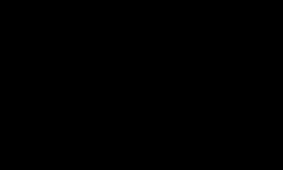
\includegraphics[width=85mm]{./imgs/im1.jpg}
\caption{\tiny{\Formular{\index{Portman, John}John Portman. {\slsc{Hotel Bonaventure}} (1976)}}}

\end{figure}

O antropólogo \index{Augé, Marc}Marc Augé (1994, p.~73) provavelmente qualificaria o
Bonaventure como um \emph{não"-lugar}, esses espaços transitórios, de
circulação e de consumo como hotéis, aeroportos e \emph{shoppings},
cujas características formais e arquitetônicas são replicadas
indistintamente em várias cidades do planeta. O \emph{não"-lugar},
segundo ele, é caracterizado por uma série de ausências: de significado,
de história, de identidade, de relação, de profundidade ---
diferentemente do \emph{lugar}, entendido como espaço antropológico, da
memória, do pertencimento, criador de identidade e incentivador das
relações interpessoais.

Se na relação com o universo das instâncias que regulam nossa vida
estabeleceu"-se uma distância intransponível, no interior do hiperespaço
pós"-moderno dá"-se uma espécie de abolição da distância, que apenas
coloca o indivíduo ``em contato com uma outra imagem de si mesmo''
(\versal{AUGÉ}, 1994, p.~73). É como se estivéssemos imersos num mundo sem a
possibilidade de enxergá"-lo com a distância crítica suficiente e,
portanto, expostos a um imediatismo paralisante.

E não podemos ser inocentes. Há uma série de interesses envolvidos nessa
desorientação espacial. Se não sabemos onde estamos, há quem se
aproveite disso. Se perdemos grande parte de nossa capacidade de
localização, isso também se deve a uma série de estratégias deliberadas
de ``deslocalização'' cujas consequências contribuirão para a atrofia de
nossa capacidade de mapeamento. Basta pensarmos nos \emph{shoppings
centers} brasileiros ou nos cassinos de Las Vegas. Esses espaços de
consumo, lazer e entretenimento são a quintessência do hiperespaço
jamesoniano acrescidos de elementos de crueldade. Nos \emph{shoppings} (que os
norte"-americanos chamam de \emph{mall}), tudo é feito para potencializar
o consumo. O projeto de iluminação elimina a consciência do dia e da
noite (uma supressão do tempo); as escadas rolantes e elevadores são
distribuídos propositalmente para a circulação infinita a fim de
provocar a passagem do sujeito pelo maior número de lojas; há toda uma
área de entretenimento e ``praças de alimentação'' para que o sujeito
prescinda da cidade, entre toda uma série de sofisticadas técnicas de
arquitetura.\footnote{Ver o documentário {\slsc{The Creators of Shopping
  Worlds}} (2001), de \index{Farocki, Harun}Harun Farocki.} O \emph{shopping} é um labirinto
ardiloso, cheio de estratégias para que o sujeito não ache a saída. Os
cassinos têm tudo isso e ainda contam com hotéis, shows, clubes
noturnos, bares, piscinas, circo, etc. Os cassinos e os \emph{shoppings} são o
exemplo definitivo de que nossa perda de capacidade de orientação
espacial não é apenas o resultado de um processo natural de
complexificação das relações, mas também um projeto deliberado de
``desmapeamento'' cujo intuito é tornar as atitudes dos seres humanos
mais previsíveis e controláveis --- um projeto de poder.

O filósofo e urbanista francês \index{Virilio, Paul}Paul Virilio, que entende a problemática
contemporânea pelo viés da velocidade, é bastante enfático ao apontar a
gravidade de tal condição.\footnote{O autor chega a propor a
  ``dromologia'', uma ciência própria para o estudo da velocidade. Ver
  \scalebox{.8}{VIRILIO}, Paul. {\slsc{Velocidade e política}}. São Paulo: Estação
  Liberdade, 1996.} Discordando da noção de ``fim da
história'',\footnote{Publicado em 1992, o livro {\slsc{O fim da história
  e o último homem}} (uma expansão de uma artigo publicado em 1989)
  identificava no fim da batalha ideológica entre o leste e o oeste a
  vitória definitiva da democracia liberal sobre os demais sistemas
  político"-econômicos.} proposta pelo cientista político norte"-americano
\index{Fukuyama, Francis}Francis Fukuyama, \index{Virilio, Paul}Virilio vaticina um ``fim da geografia'', causado pela
compressão temporal ou pelo que chama de ``aceleração da realidade''.
Para ele (\versal{VIRILIO}, 1993, p.~13), nesse contexto de ubiquidade e
instantaneidade, a noção conjunta de velocidade e distância supera a
própria dimensão física, abolindo tempo e espaço. Quem está em todos os lugares ao mesmo tempo está, na verdade, em lugar nenhum.

\chapter{Justa medida}

Podemos então perceber que o ciberespaço e o hiperespaço, esses dois
novos ambientes contemporâneos, comportam"-se de maneiras distintas, mas
complementares. A imersão acrítica induzida pelo hiperespaço impede que
enxerguemos as complexas relações espaciais que constituem o mundo
contemporâneo, representadas pela teia do ciberespaço.

Por analogia, também é possível compreendermos esses ambientes à luz da
distinção conceitual proposta por \index{Deleuze, Gilles}Gilles Deleuze e \index{Guattari, Félix}Félix Guattari entre
\emph{espaço liso} e \emph{espaço estriado}. Uma leitura
estrutural poderia definir o ciberespaço como ``espaço sem fronteiras,
não cercado'', um lugar sem ``perspectiva nem contorno'' onde ``qualquer
ponto pode ser conectado a qualquer outro''. Do ponto de vista do
deslocamento, a navegação pela rede se daria através da ``variação
contínua de suas orientações, referências e junções'' deixando pelo
caminho apenas ```traços' que se apagam e se deslocam com o trajeto''.
Este ciberespaço, difícil de compreender visualmente, seria o espaço das
``multiplicidades não métricas, acentradas, rizomáticas'', onde tudo é
trajeto, vetor, direção e nada é mensurável. Pois essas são justamente
as definições de \emph{espaço liso} colocadas por \index{Deleuze, Gilles}Deleuze e Guattari. A
interpretação otimista dessas definições leva o sujeito incauto a
enxergar na rede de computadores o espaço utópico da conexão entre os
povos, um mundo ``ao alcance dos dedos'' onde todos falam a mesma
língua. Mas os próprios autores, embora enxerguem na ocupação do
\emph{espaço liso} a possibilidade de transformação positiva da
sociedade, tratam de advertir que, no fundo, ele é apenas o palco onde
as lutas por essa libertação serão travadas, onde ``a vida reconstitui
seus desafios, afronta novos obstáculos, inventa novos andamentos,
modifica os adversários'' (\versal{DELEUZE}; \versal{GUATTARI}, 2012, p.~228).

Portanto, é preciso ter cuidado. O \emph{espaço liso}, apesar da vocação
revolucionária, não garante a ocupação positiva do território, podendo
ser \emph{estriado} pelo Estado ou ``traçado e ocupado por potências de
\emph{organização} diabólicas'' (2012, p.~200), exatamente como nas
novelas \emph{cyberpunk}.

Por outro lado, o ambiente de sufocamento imersivo do hiperespaço
sugere delimitações e repartições ``segundo intervalos
determinados, conforme cortes assinalados''. O Hotel Bonaventure, um
\emph{shopping center}, uma novela de \index{Kafka, Franz}Kafka, podem ser considerados espaços
\emph{estriados}, ``por muros, cercados e caminhos entre os cercados'',
onde os homens são distribuídos em espaços fechados, onde a percepção é
feita de ``medidas e propriedades''. Aqui é preciso ``constância da
orientação, invariância da distância por troca de referenciais de
inércia''.\footnote{\scalebox{.8}{DELEUZE}; \scalebox{.8}{GUATTARI}, 2012, passim.}

Essas duas situações espaciais apontam para uma mesma conclusão
preocupante. O deslocamento espacial do corpo não significa
necessariamente acesso aos lugares distantes e diferentes, da mesma
forma que o simples acesso a esses lugares não garante o deslocamento do
sujeito. ``Ubiquidade e imediaticidade são nada mais do que \label{ubiquidade}
imobilismo'', diria \index{Virilio, Paul}Virilio (2012, p.~65). No ciberespaço o sujeito tem
a ilusão de acesso a todos os lugares instantaneamente e
simultaneamente, mas na realidade está imóvel diante do computador ou
imerso na tela do \emph{smartphone}, alheio ao mundo ao redor ou, para usar os termos de Baudrillard (1997, p. 147), em ``interação em tempo real com o vazio''. No
hiperespaço claustrofóbico, quanto mais esse mesmo sujeito se desloca em
redundância espacial, mais roda em falso no mesmo lugar. Nos dois casos,
um falso movimento.

O sociólogo e filósofo francês Jean Baudrillard (1983, p.~133, trad.~minha), já nos anos \label{internet} 1980, percebia os perigos dessa imersão acrítica, que chamou de ``êxtase da comunicação'', um sistema onde ``todos os segredos, espaços e cenas são abolidos numa única dimensão de informação''. Com isso nasce um novo ser esquizofrênico e promíscuo, caracterizado pela ``proximidade absoluta, a total instantaneidade das coisas, a ausência de defesa e de refúgio''. Um ser que precisa encarar ``o fim da interioridade e da intimidade, a superexposição e a transparência do mundo, que nos atravessa sem obstáculo''.

Posteriormente, Baudrillard (1998, p.~12) enxergou na internet o veículo contemporâneo paradigmático dessa perda de distância. Segundo ele (para quem a comunicação hoje não passa de ``um grande fenômeno consumista''), estamos submersos num oceano virtual de infinitas possibilidades, onde não há mais distinção entre conhecimento e informação, onde uma massa avassaladora de dados nos torna escravos passivos de um sistema informático.

O problema da distância crítica entre o homem e o objeto observado por
ele vem sendo diagnosticado pelo menos desde os anos 30 do século \versal{XX},
quando \index{Benjamin, Walter}Walter Benjamin escreve o célebre ensaio \emph{A obra de arte na \label{benjamin}
era de sua reprodutibilidade técnica}. Segundo ele (1985, p.~167), com a
possibilidade de reprodução técnica da obra de arte proporcionada pela
fotografia e pelo cinema, a obra passa de uma existência única para uma
existência em série, colocando em xeque as noções de autenticidade e
originalidade. Isso elimina o ``aqui e agora'' da obra de arte e encurta
a distância entre o espectador e o objeto. \index{Benjamin, Walter}Benjamin chama isso de
``destruição da aura'', um fenômeno que, ao reduzir esse ``valor de
culto'' do objeto artístico, direcionaria sua função para um sentido
mais social. Essa ``popularização'' da arte, no entanto, traz perigos. O
cinema, diz \index{Benjamin, Walter}Benjamin, com seu poder de sedução, pode mobilizar as massas
mas também, justamente por isso, pode abrir caminho para o fascismo, que
soube utilizar com eficácia a reprodução técnica como
propaganda.\footnote{O texto de \index{Benjamin, Walter}Benjamin é contemporâneo dos filmes de
  propaganda nazista dirigidos por \index{Riefenstahl, Leni}Leni Riefenstahl como {\slsc{Triunfo
    da vontade}} (1934) e {\slsc{Olympia}} (1938), cujas inovações técnicas
  são inegáveis.} Em suma, \index{Benjamin, Walter}Benjamin (1987, p.~54) enxerga com entusiasmo essa nova
proximidade entre o observador e o objeto observado pelo seu potencial
popular e revolucionário, mas também percebe que, ao reduzir"-se a
distância conceitual, a distância crítica também é prejudicada. E
crítica é, para \index{Benjamin, Walter}Benjamin, justamente ``uma questão de
correto distanciamento''.

Distanciamento crítico e suas implicações políticas são também uma \label{brecht}
questão central no teatro de \index{Brecht, Bertolt}Bertolt Brecht. Através de revelação dos
mecanismos cênicos do teatro o autor buscava sempre lembrar ao público
que ele não estava diante de uma imitação da realidade, mas de uma obra
teatral, de uma representação artificial da realidade. Música, humor,
placas, comentários em cena, olhares direcionados à plateia ignorando a
``quarta parede'' impediam a identificação do público com os personagens
e a contemplação passiva do espetáculo. \index{Brecht, Bertolt}Brecht chamava isso de
\emph{Verfremdungseffekt} (efeito de distanciamento), cujo resultado
seria o ``correto distanciamento'' crítico. O chamado teatro épico de
\index{Brecht, Bertolt}Brecht no fundo estava ligado a um projeto político socialista que tinha
como objetivo dotar o homem de consciência de sua própria capacidade de
transformação da sociedade.

Assim como \index{Benjamin, Walter}Benjamin, é também através da observação dos avanços
tecnológicos que \index{Heidegger, Martin}Martin Heidegger, já em 1947, percebe a supressão
relativa das distâncias. Para o filósofo alemão, o avião, o rádio, o
cinema e, sobretudo, a televisão, relativizaram de maneira dramática as
noções de perto e longe. O homem agora é capaz de colocar diante de si,
a uma distância mínima, a totalidade das coisas. \index{Heidegger, Martin}Heidegger (1994, p.~144) identifica o problema que os pensadores do pós"-modernismo vão
desenvolver décadas depois: ``o que acontece quando, suprimindo as
grandes distâncias, tudo se torna igualmente próximo e igualmente longe?\footnote{\index{Foster, Hal}Hal Foster (1993) enxerga três momentos nesse processo de
  supressão do distanciamento crítico causado pelo impacto da tecnologia
  ao longo do século \scalebox{.8}{XX}: a era benjaminiana da reprodução mecânica dos
  anos 1930, a era da revolução cibernética dos anos 1960 (descrita por
  \index{Debord, Guy}Guy Debord e \index{McLuhan, Marshall}Marshall McLuhan) e a era da tecnocultura dos anos 1990.}
Em que consiste essa uniformidade em que nada está nem perto nem longe,
como se não houvesse distância?''.

O que se percebe é que, se a relação homem"-espaço se manteve
relativamente estável historicamente, agora a humanidade se vê diante de
um problema que não existia. Essa espécie de falha em nossa percepção do
entorno, que nos anos 1990 chega a ponto dramático, é, na verdade, o
resultado de um processo que se inicia anteriormente, segundo os
próprios pensadores do pós"-modernismo: ``em sociedades mais antigas, e
talvez até nos primeiros estágios do capitalismo de mercado, a
experiência limitada e imediata dos indivíduos ainda é capaz de abranger
e coincidir com a verdadeira forma social e econômica que regula essa
experiência, no momento seguinte os dois níveis se afastam e começam a
se constituir naquela oposição que a dialética clássica descreve como
\emph{Wesen} e \emph{Erscheinung}, essência e aparência, estrutura e
experiência do vivido'' (\versal{JAMESON}, 2000, p.~406).

De forma semelhante, Paul \index{Virilio, Paul}Virilio (1993, p.~76) aponta na mesma direção.
Para ele, já não se pode falar mais em aceleração nem em redução das
distâncias, mas em ``abolição do espaço''. Até o século \versal{XIX} esse espaço
ainda era ``semelhante a si próprio'' mas agora desaparece diante de um
\emph{espaço"-velocidade} sem dimensão, em que a grandeza da velocidade
surge como padrão de todo dimensionamento.

Ainda na mesma linha, para \index{Harvey, David}David Harvey (2014, p.~238), as revoluções políticas,
sociais e técnicas do século \versal{XIX}, proporcionaram uma integração espacial
da realidade europeia sem precedentes. A manipulação virtual do dinheiro
e o novo internacionalismo criaram uma situação onde ``a certeza do
espaço e do lugar absolutos foi substituída pelas inseguranças de um
espaço relativo em mudança, em que os eventos de um lugar podiam ter
efeitos imediatos e ramificadores sobre vários outros''.
Some"-se a isso a evolução das velocidades de transporte e comunicação,
temos o que \index{Harvey, David}Harvey chamou de \emph{compressão do tempo"-espaço}, ou seja,
um encurtamento relativo das distâncias decorrente do aumento das
velocidades de deslocamento e da informação. Nessa nova condição de
``aldeia global'', um evento acontecido num lugar tem um impacto
imediato sobre pessoas e lugares situados a uma grande distância desse
lugar.\footnote{``Aldeia global'' é o famoso termo cunhado nos anos 1960
  pelo filósofo canadense \index{McLuhan, Marshall}Marshall
  McLuhan para referir"-se aos efeitos da comunicação de massa sobre a
  sociedade contemporânea, antevendo a globalização generalizada dos
  anos 1990.}

Nesse contexto, a distância deixa de ser um dado físico, objetivo ou
impessoal para ser um ``produto social'' cuja extensão varia dependendo
da velocidade com a qual pode ser vencida, do custo envolvido na
produção dessa velocidade e da classe social a que pertence o
indivíduo.\footnote{``Para os habitantes do Primeiro Mundo --- o mundo
  cada vez mais cosmopolita e extraterritorial dos homens de negócio
  globais, dos controladores globais da cultura e dos acadêmicos globais
  --- as fronteiras dos Estados foram derrubadas, como o foram para as
  mercadorias, o capital e as finanças. Para os habitantes do Segundo
  Mundo, os muros constituídos pelos controles de imigração, as leis de
  residência, a política de ``ruas limpas'' e ``tolerância zero''
  ficaram mais altos; os fossos que os separam dos locais de desejo e da
  sonhada redenção ficaram mais profundos''. Ver \scalebox{.8}{BAUMAN},
  Zygmunt. {\slsc{Globalização: as consequências humanas}}. Rio de
  Janeiro: Zahar, 1999, p.~97.} É por isso que não podemos nos deixar
levar facilmente pelo discurso dos entusiastas da tecnologia, que
acreditam no encurtamento puro e simples da distância, enxergando apenas
a facilidade prática que isso representa. Se, por um lado isso de fato
acontece, por outro as distâncias entre o indivíduo e as instâncias de
poder (muitas vezes relativas ao próprio universo da tecnologia) apenas
aumentaram.

\begin{figure}[!ht]

\centering
 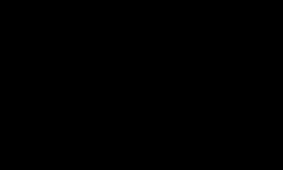
\includegraphics[width=85mm]{./imgs/im1.jpg}
\caption{\tiny{\Formular{Reuters. Trens de alta velocidade, Wuhan, China (2012)}}}

\end{figure}

\index{Harvey, David}Harvey demonstra que essa revolução já acontecia desde o século \versal{XIX} e é
parte integrante do próprio modo de funcionamento do capitalismo. O
próprio \index{Marx, Karl}Marx (apud \versal{HARVEY}, 2014, p.~298) já havia percebido que ``é da natureza do capital mover"-se
para além de todas as barreiras espaciais. A criação das condições
físicas de troca --- de meios de comunicação e transporte --- devém uma
necessidade para o capital em uma dimensão totalmente diferente --- a
anulação do espaço pelo tempo''.

Esse modelo de funcionamento teve um novo impulso no final do século \versal{XX}.
O geógrafo defende que, se o modernismo foi uma resposta à nova condição
espacial surgida no século \versal{XIX}, o pós"-modernismo seria uma resposta à
uma nova rodada da compressão do tempo"-espaço decorrente da passagem do
regime fordista de produção para um sistema de acumulação flexível,
ocorrido a partir dos anos 1970. Nesse novo contexto geopolítico, os
conflitos globais muitas vezes serão disputas por espaço, não mais como
território físico a ser conquistado por um exército, mas como arena de
atuação do poder gerado pelo capital que, muitas vezes, vai se confundir
com as redes virtuais ou com o próprio mercado financeiro. O domínio
sobre esses espaços vai se tornar, portanto, fundamental para qualquer
projeto de poder, e sua conquista vai exigir capacidade, treinamento e
disciplina, como numa campanha militar. Nesse contexto, a informação
``geovirtual'' precisa (como um mapa) vai se tornar mercadoria
essencial.

\chapter{O rato no labirinto}

Estamos, portanto, diante de um problema de ordem espacial. Se a
indagação quintessencial da modernidade, resumida por \index{Gauguin, Paul}Paul Gauguin, era
``de onde viemos? o que somos? para onde vamos?'', a pergunta
existencial mais premente da pós"-modernidade e, por extensão, do mundo
contemporâneo, talvez seja ``onde estamos?''.\footnote{{\slsc{De onde
  viemos? O que somos? Para onde vamos?}} é literalmente o título de uma
  enigmática tela de \index{Gauguin, Paul}Gauguin pintada no Taiti em 1897, que pode ser
  interpretada como uma alegoria de um ``paraíso perdido'' existencial.
  O pintor considerava a tela como sua melhor obra e escreveu que
  pensava em cometer suicídio enquanto pintava.} E, se nossa noção de
espaço se expandiu e passou a abranger esses novos espaços virtuais de
atuação humana, essa pergunta não se responde mais com nossas
coordenadas geográficas sobre a superfície do planeta. De fato, vivemos
uma contradição bastante espantosa em que o mundo nunca foi tão bem
mapeado (penso nas plataformas digitais cartográficas como o
\emph{Google Maps}) ao mesmo tempo em que o homem vai perdendo cada vez
mais sua capacidade de localização.

\begin{figure}[!ht]

\centering
 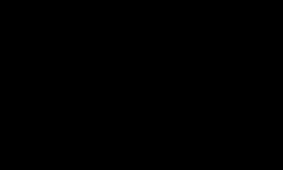
\includegraphics[width=85mm]{./imgs/im1.jpg}
\caption{\tiny{\Formular{\index{Tolman, Edward}O labirinto de Tolman e o gráfico que\break mostra a curva de erros dos ratos}}}

\end{figure}

Nossa situação espacial não é mais apenas um dado objetivo e mensurável.
Não é mais um alfinete num mapa de parede e vai nos exigir uma nova
postura em relação ao mundo. Essa complexa situação foi bem percebida
pelo filósofo francês \index{Rancière, Jacques}Jacques Rancière (2009, p.~115, trad.~minha):

\begin{quote}
``Onde estamos?'' significa duas coisas ao mesmo tempo: ``como podemos
caracterizar a situação em que vivemos, pensamos e agimos hoje'', mas
também, da mesma forma: ``como a percepção dessa situação nos obriga a
reconsiderar o enquadramento que usamos para `ver' as coisas e mapear
situações, para movermo"-nos dentro desta estrutura ou escapar dela?'';
ou, em outras palavras, ``como nos obriga a mudar nossa própria maneira
de determinar as coordenadas do `aqui e agora?'".
\end{quote}

Percebemos então que essa pergunta, diferentemente das outras grandes
perguntas existenciais, é a que sofreu maior abalo nas últimas décadas.
A própria noção inquestionável de ``aqui e agora'' sofreu um grande
abalo. Se antes tínhamos um problema de identidade, agora temos um
problema de ordem espacial. Se antes o problema estava no \emph{eu},
agora foi deslocado para o mundo.\footnote{O sociólogo jamaicano \index{Hall, Stuart}Stuart
  Hall (2006) aborda o tema da ``morte do sujeito'' na pós"-modernidade.
  Para ele, o ``indivíduo soberano'', centrado e indivisível, nascido
  entre o Renascimento e o Iluminismo, foi ``descentrado'' ao longo dos
  séculos \scalebox{.8}{XIX} e \scalebox{.8}{XX}, resultando nas identidades abertas, contraditórias,
  inacabadas e fragmentadas do sujeito pós"-moderno. \index{Hall, Stuart}Hall identifica
  cinco ``descentramentos'' fundamentais: o marxismo, a descoberta do
  inconsciente por Freud, a linguística moderna de \index{Saussure, Ferdinand de}Saussure, o ``poder
  disciplinar'' descrito por \index{Foucault, Michel}Foucault e o feminismo.} Michel Foucault
(1994, p.~752, trad.~minha) é
um dos pensadores que atestam essa primazia do espaço no mundo
contemporâneo. Na famosa conferência \emph{De outros espaços},\footnote{Conferência
  pronunciada no Círculo de Estudos Arquitetônicos, em Paris, no dia 14
  de março de 1967. \index{Foucault, Michel}Foucault autorizou sua publicação apenas em 1984,
  pouco tempo antes de sua morte, no contexto da exposição {\slsc{Ideia,
    processo, resultado}}, parte da programação da {\slsc{Internationale
      Bauausstellung}} (\scalebox{.8}{IBA}), em Berlim. A conferência, por sua vez, é
  derivada de duas emissões radiofônicas proferidas por \index{Foucault, Michel}Foucault nos
  dias 7 e 21 de dezembro de 1966. Ver \scalebox{.8}{FOUCAULT}, Michel. {\slsc{O corpo
    utópico, as heterotopias.}} São Paulo: n"-1, 2013.} refere"-se claramente
a essa mudança:

\begin{quote}
A nossa época talvez seja sobretudo a época do espaço. Nós estamos na
época da simultaneidade, nós estamos na época da justaposição, na época
do próximo e do distante, do lado"-a"-lado, do disperso. Acredito que
estamos num momento no qual a nossa experiência do mundo se assemelha
menos com uma longa via que se desenvolve através do tempo do que com
uma rede que conecta os pontos e se intersecta em sua própria trama.
\end{quote}

Vivemos, portanto, num mundo muito mais regido pela sincronia do que
pela diacronia, onde, por exemplo, a simultaneidade da imagem substituiu
a sequencialidade da leitura. De fato, nos últimos anos houve uma
mudança de rota nos estudos de humanidades, com uma ênfase maior no
estudo do espaço, tornando"-se agora uma categoria analítica tão
importante quanto o tempo. Das distinções de \index{Certeau, Michel de}Michel de Certeau acerca
dos conceitos de ``espaço'' e ``lugar'' aos delírios
enciclopédicos de \index{Perec, Georges}Georges Perec; dos espaços ``lisos'' e ``estriados'' de
\index{Deleuze, Gilles}Deleuze e Guattari ao ``não"-lugar'' de \index{Augé, Marc}Marc Augé; do \emph{terrain
vague} de \index{Solà-Morales, Ignasi de}Solà"-Morales ao ``hiperespaço'' de Fredric \index{Jameson, Fredric}Jameson, esse
campo de interesse trará uma série de novidades para o universo da
filosofia e das artes, ampliando seus escopos de atuação. Eles não
deixam dúvida de que será preciso compreender o mundo a partir de uma
nova \emph{geografia}.

Diagnosticado o problema da lacuna entre o homem e o espaço
contemporâneo, um dos projetos mais ambiciosos da contemporaneidade
seria o de recuperar a capacidade de situarmo"-nos relacionalmente nesse
espaço. Trata"-se de uma capacidade que parece ter sido perdida em algum
momento da história. É por isso que \index{Augé, Marc}Marc Augé (1994, p.~37) ao perceber que ``o mundo
da supermodernidade não tem as dimensões exatas daquele no qual
pensamos viver'' alerta simplesmente sobre a necessidade de
``reaprender a pensar o espaço''.

Fredric \index{Jameson, Fredric}Jameson desenvolve uma espécie de solução para esse problema a
partir do conceito de ``mapeamento cognitivo''.\footnote{\index{Jameson, Fredric}Jameson utiliza
  pela primeira vez o termo no ensaio {\slsc{Postmodernism, or, the
    Cultural Logic of Late Capitalism}}, publicado originalmete em 1984 na
  revista {\slsc{New Left}}. O ensaio foi posteriomente publicado como o
  primeiro capítulo do livro de mesmo nome, em 1991.} O termo
propriamente dito provém do universo da neurociência, e foi
primeiramente usado pelo psicólogo \index{Tolman, Edward}Edward Tolman no estudo
\emph{Cognitive maps in rats and men}, publicado em 1948.\footnote{Publicado na
  revista {\slsc{The Psychological Review}}, 55(4), 1948, pp.~189-208.} O
experimento envolvia o estudo do comportamento de ratos de laboratório
em busca de alimento dentro de labirintos artificiais. \index{Tolman, Edward}Tolman percebeu
que os animais cometiam cada vez menos erros quanto mais repetiam os
caminhos e se familiarizavam com o labirinto. O experimento sugeria que
os ratos eram capazes de ``memorizar'' o espaço, criando uma espécie de
``mapa mental''. Trata"-se, portanto, de um processo de estruturar e
armazenar informações espaciais que os cientistas acreditam acontecer
numa área do cérebro conhecida como hipocampo. Essa estrutura cerebral
presente nos humanos e em outros mamíferos é considerada a maior
responsável pela nossa capacidade de espacialização. Dessa forma, essa
não seria uma capacidade exclusiva dos seres humanos. Para os animais,
inclusive, o mapeamento cognitivo estaria diretamente ligado à própria
sobrevivência, podendo ser questão de vida ou morte.\footnote{Mais
  recentemente o termo tem sido evitado por alguns cientistas no que diz
  respeito à capacidade animal de leitura do espaço. Embora os animais
  tenham sem dúvida um sistema de navegação que os orienta, para esses
  cientistas esse sistema não configura exatamente um mapeamento
  (\scalebox{.8}{BENNET}, 1996).}

No universo da neurociência, esse tipo de mapeamento pode ser definido
como ``representações de indícios visuais, táteis, auditivos, que
configuram o ambiente e permitem a localização do sujeito no espaço''
(\index{Bastos, Antonio}\versal{BASTOS}, 2002). Para o filósofo brasileiro \index{Peixoto, Nelson Brissac}Nelson Brissac Peixoto (1996, p.~408), o mapeamento é um modo de percepção não"-ocular que se configura
através da fusão do real e do abstrato, sendo ``a primeira imagem de uma
paisagem que não pode ser apreendida diretamente pelo olho''.

\index{Jameson, Fredric}Jameson desenvolve o conceito identificando a convergência de duas
fontes aparentemente distintas, sendo uma prática e outra teórica: de um
lado, os estudos de campo do urbanista \index{Lynch, Kevin}Kevin Lynch e, do outro, o
conceito de ideologia conforme proposto por \index{Althusser, Louis}Louis Althusser.

A pesquisa que \index{Lynch, Kevin}Lynch realizou nos anos 50 resultou num livro clássico
dos estudos urbanos: \emph{A imagem da cidade} (1960). Partindo de
pesquisas de campo em três cidades norte"-americanas (Boston, Jersey City
e Los Angeles), o autor estabeleceu critérios de qualidade urbana com
base na ``legibilidade'' e na ``imaginabilidade'' da cidade, ou seja, na
capacidade de a cidade criar uma imagem mental de seus espaços que
pudesse ser retida com vigor na memória de seus habitantes. Para ele,
uma cidade ``legível'' é aquela que gera uma estrutura de símbolos
urbanos reconhecíveis, facilmente identificáveis e passíveis de
agrupamento. Quanto mais ``legível'' for essa cidade, mais conforto,
segurança e prazer ela oferece, intensificando a profundidade e a
intensidade da experiência urbana de seus habitantes. A novidade do
livro era sua concepção de cidade eminentemente fenomenológica, com base
na percepção individual e subjetiva dos cidadãos, diferentemente dos
estudos da época, que percebiam a cidade sobretudo pelo prisma de sua
configuração geométrica.

\begin{figure}[!ht]

\centering
 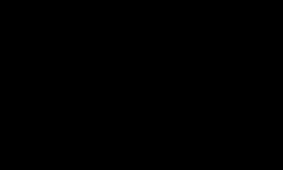
\includegraphics[width=85mm]{./imgs/im1.jpg}
\caption{\tiny{\Formular{\index{Lynch, Kevin}Kevin Lynch. Ilustrações do livro {\slsc{A imagem da cidade}}}}}

\end{figure}

Além de demonstrar a importância da imagem subjetiva da cidade para o
planejamento urbano, \index{Lynch, Kevin}Lynch (1980, p.~132) sugere uma relação de mão
dupla entre a legibilidade do espaço e a ação sobre o ambiente. Para
ele, a ``educação visual'' é o instrumento que o cidadão precisa para
modificar o mundo. Modificado, ele se torna mais nítido e claro,
contribuindo para a ``educação visual''.

Localização, posicionamento, individuação, identificação e delimitação
são operações que têm um papel chave na formação das subjetividades
pessoais e políticas. Aquilo que somos é determinado em larga medida por
nossa localização na sociedade e no mundo. Portanto, uma percepção
adequada de nosso entorno e de nosso posicionamento relativo na cidade e
no mundo é fundamental tanto para a identidade individual quanto para a
noção de coletividade. Fundamentalmente, se não somos capazes de ``ler''
ou mapear mentalmente a cidade, não podemos agir sobre ela; se não
podemos agir sobre ela, estamos construindo uma experiência alienada e
alienante, contrária a qualquer noção responsável de cidadania. Para
\index{Jameson, Fredric}Jameson (2000, p.~77), a desalienação no contexto urbano envolveria
então a ``reconquista prática de um sentido de localização e de
reconstrução de um conjunto articulado que pode ser retido na memória'',
e que pode ser mapeado e remapeado conforme o deslocamento.

A um pensador marxista como \index{Jameson, Fredric}Jameson interessa muitíssimo o aspecto
político da proposta de \index{Lynch, Kevin}Lynch, pois enxerga nela um potencial de
extrapolação da análise espacial para o domínio da estrutura social.
\index{Jameson, Fredric}Jameson parte do pressuposto de que a impossibilidade de mapear
espacialmente é tão debilitadora para a experiência urbana quanto a
incapacidade análoga de mapeamento social para a experiência política.
Se, na conhecida definição de \index{Althusser, Louis}Althusser (1970, p.~77), a ideologia
``representa a relação imaginária dos indivíduos com as suas condições
reais de existência'', então a proposta de legibilidade do meio urbano
que \index{Lynch, Kevin}Lynch desenvolveu para a cidade poderia (e deveria) ser expandida e
aplicada em relação ao mundo como um todo. A dialética entre o ``aqui e
agora'' da percepção imediata da experiência urbana e o sentido
imaginário e imaginativo da cidade proposta por \index{Lynch, Kevin}Lynch seria uma espécie
de ``análogo espacial'' da definição de \index{Althusser, Louis}Althusser. O objetivo comum
seria preencher a lacuna que separa a localização espacial do indivíduo
e a realidade das estruturas de poder em que ele se situa.

Este é o cerne da proposta de mapeamento cognitivo, cuja função seria
``permitir a representação situacional por parte do sujeito individual
em relação àquela totalidade mais vasta e verdadeiramente
irrepresentável que é o conjunto das estruturas da sociedade como um
todo'' (2000, p.~77). O problema, portanto, não é tanto a
\emph{incognoscibilidade} do novo sistema mundial do capitalismo global,
mas sua \emph{irrepresentabilidade} (daí o mérito do \emph{cyberpunk}
que, embora deficiente, é uma tentativa legítima de representar essas
novas relações de poder). Antes de podermos agir, devemos criar uma
imagem mental dessa totalidade global ou social que todos temos na
cabeça de forma confusa --- um exercício que guarda relação com aquele
exigido do rato em busca do alimento no labirinto de \index{Tolman, Edward}Tolman. Imagem
mental é a própria definição simplificada de mapeamento cognitivo, cuja
função última seria criar uma representação do mundo, não exatamente com um mapa gráfico limitado às suas duas dimensões, mas muito mais complexa, de difícil visualização, para a qual talvez ainda não tenhamos (ou já tenhamos perdido) o ``equipamento perceptivo'' necessário.


O primeiro passo seria, justamente, descartar a própria ideia do mapa,
apesar de pertencer ao mesmo campo semântico da ideia de mapeamento.
Esse poderoso, extraordinário e sedutor instrumento científico, com toda
sua simplicidade enganadora, no fundo atrofia (ou mesmo anula) nossa
capacidade de mapear o espaço de forma autônoma e crítica. Na mesma
linha de raciocínio, \index{Harvey, David}David Harvey (2001, p.~221) reconhece a existência
de ``mapas mentais ou cognitivos (talvez sistemas cartográficos
inteiros) embutidos em nossa consciência que desafiam representações
simplistas num `grid' cartesiano''.

A estética do mapeamento cognitivo vai exigir um enorme poder de
abstração, uma maneira estratégica de estranhamento e distanciamento dos
fenômenos:

\begin{quote}
Uma estética do mapeamento cognitivo --- uma cultura política e
pedagógica que busque dotar o sujeito individual de um sentido mais
aguçado de seu lugar no sistema global --- terá, necessariamente, que
levar em conta essa dialética representacional extremamente complexa e
inventar formas radicalmente novas para lhe fazer justiça. Esta não é,
então, uma convocação para a volta a um tipo mais antigo de aparelhagem,
a um espaço nacional mais antigo e transparente, ou a qualquer enclave
de uma perspectiva mimética mais tradicional e tranquilizadora: a nova
arte política (se ela for de fato possível) terá que se ater à verdade
do pós"-modernismo, isto é, a seu objeto fundamental --- o espaço mundial
do capital multinacional --- , ao mesmo tempo que terá que realizar a
façanha de chegar a uma nova modalidade, que ainda não somos capazes de
imaginar, de representá"-lo, de tal modo que nós possamos começar
novamente a entender nosso posicionamento como sujeitos individuais e
coletivos e recuperar nossa capacidade de agir e lutar, que está, hoje,
neutralizada pela nossa confusão espacial e social. A forma política do
pós"-modernismo, se houver uma, terá como vocação a invenção e a projeção
do mapeamento cognitivo global, em uma escala social e espacial
(\versal{JAMESON}, 2000, p.~79).
\end{quote}

Portanto, essa revalorização da experiência não é um chamado regressivo
a antigas formas de reconhecimento do território numa chave nostálgica,
querendo recuperar uma época em que a escala do mundo e a escala humana
ainda se relacionavam de forma harmoniosa. Quanto a isso, não há volta.
É, ao contrário, uma proposta crítica e de resistência, um gesto
político que não aceita passivamente a condição alienante da cidade e do
mundo como ela se apresenta.

De forma mais prática, trata"-se de uma visualização panorâmica de toda a cadeia de pequenos eventos que compõe os grandes eventos.\footnote{O filósofo inglês \index{Morton, Timothy}Timothy Morton cunhou o termo ``hiperobjeto'' para descrever fenômenos tão grandes e complexos que escapam à compreensão humana. Entre esses objetos estariam os buracos negros, a biosfera, a internet e, sobretudo, o aquecimento global. Ver \scalebox{.8}{MORTON}, Timothy. {\slsc{Introducing the idea of ‘hyperobjects’: A new way of understanding climate change and other phenomena}}. High Country News, Paonia, p.~8-9, 19 jan. 2015.} Por exemplo: ter clara compreensão da origem e do destino do dinheiro utilizado nos financiamentos de campanhas políticas, percorrer o caminho do minério de ferro desde sua extração no Pará até o uso do aço na construção chinesa, acompanhar o caminho do dinheiro utilizado na aquisição milionária de uma obra de arte, conhecer as relações entre política e direito para saber as motivações de determinada decisão de um juiz, saber onde e como são armazenados os dados de bilhões de usuários da internet colhidos pelas empresas de tecnologia e qual seu verdadeiro uso, entre tantos outros.

Uma forma bastante eficaz de esconder a verdade é a fragmentação dos eventos de forma que não se possa mais juntar os pedaços, a não ser por aqueles que a fragmentaram. Daí a necessidade de uma método emancipatório de ação que tenha por objetivo justamente a reconexão das partes com o todo. Nessse sentido, apesar de todo esforço de especialização em determinados assuntos, precisamos também daqueles capazes de juntar as partes, recolher os cacos, soldar os fios e prencher as fissuras.

Para \index{Jameson, Fredric}Jameson, ainda mais do que um projeto político, o mapeamento
cognitivo é ``parte integral de qualquer projeto político socialista'',
uma vez que incrementaria nossa ``consciência geopolítica'' e nos
forneceria elementos para atuarmos no ambiente como forma de
defendermo"-nos das estruturas de poder. No centro de sua preocupação
está a desalienação do indivíduo diante das estruturas opressivas,
ilegíveis e irrepresentáveis do mundo contemporâneo, associadas ao
capitalismo. Mapeamento cognitivo seria, nessa perspectiva, uma espécie
de código para uma nova ``consciência de classe'', um projeto
emancipatório diante das injustiças do mundo capitalista, e um modo de
superá"-lo.

Os estudiosos em geral são bastante argutos ao apontar os problemas do
mundo contemporâneo, mas poucos são capazes de indicar uma saída para as
mesmas situações que descrevem. Se o diagnóstico dos males do mundo
contemporâneo vem sendo feito com eficiência há algum tempo, falta"-lhe a
prescrição para o tratamento. O projeto de mapeamento cognitivo pode ser
extremamente ambicioso, teórico, e utópico, mas tem o mérito inegável de
buscar uma solução onde tudo parece esgotado --- uma situação que
pensadores como \index{Bauman, Zygmunt}Zygmunt Bauman e \index{Berardi, Franco}Franco Berardi vêm chamando de ``fim do
futuro''.

Mas por que razão isso acontece? Por que o futuro nos parece tão
nebuloso? Se levarmos em conta que o futuro é sempre uma espécie de
projeto (ou de sonho) teremos que fazer uso da imaginação para poder
construí"-lo. E a imaginação é uma matéria"-prima humana bastante em
falta. O excesso de informação, os espaços hiperestimulantes e o
bombardeio de imagens ocupam toda nossa atenção, prejudicando gravemente
nossa capacidade de imaginação. Lutar contra isso deveria ser um projeto
urgente.

Talvez o primeiro passo seja aceitar o ``fracasso representacional''
inerente à complexidade da realidade contemporânea. Essa resignação
teria ao menos a virtude de evidenciar a insuficiência da cartografia e
dos dispositivos tradicionais de localização, além de admitir que há limites naquilo que a própria mente humana é capaz de conceber. Apenas abandonando essas formas tradicionais de
representação poderemos abrir caminho para novas e ainda insuspeitadas
maneiras de mapear essa realidade que nos foge do campo de visão.

Outro passo importante é rejeitar as narrativas simplificadoras, mesmo diante da enorme complexidade que temos que enfrentar. Um dos grandes males de nossa época é justamente a redução das complexidades a uma mensagem facilmente apreensível, que exige menor esforço mental. É a fórmula usada pelo populismo e pelas teorias conspiratórias, que escondem os problemas e adiam sua resolução para as gerações seguintes. 

A ideia de um mapeamento cognitivo talvez seja apenas mais uma utopia,
cuja força vibrante reside --- como em toda utopia --- justamente em sua
impossibilidade. A utopia tem como função virtuosa manter o futuro vivo,
aberto às transformações da história. Projetos utópicos como o
mapeamento cognitivo são, em última análise, um gesto de resistência
diante do perigo desse ``fim do futuro'' que se anuncia de forma
alarmante. Projetos como esse devem ser perseguidos, mesmo sob o risco
do fracasso total, mesmo que no final desapareçam como ``lágrimas na
chuva''.


\partepigraph{It is not down in any map; true places never are}{\index{Melville, Herman}Herman Melville, \emph{Moby Dick} (1851)}
\part{Mapas, territórios}
\removeepigraph

\chapter{Você está aqui}

O mapa é um dos mais revolucionários e fascinantes instrumentos
científicos já inventados pelo homem. Desde as primeiras representações
do território inscritas na pedra até as plataformas digitais atualizadas
a todo instante, o mapa tem mudado e condicionado nossa compreensão do
mundo.

O mapa pode nortear um viajante ou ser o causador de intensa disputa
política; pode orientar um motorista de uma grande cidade ou servir de
inspiração para os artistas; pode ser usado como instrumento de poder ou
de imaginação. Além disso, o mapa possui uma beleza própria, sendo um
objeto gráfico que estimula a criatividade de quem o produz ao permitir
o uso incrivelmente diverso de desenhos, cores, nomes e símbolos. Ao
confeccionarmos um mapa, atribuímos valores simbólicos e estéticos ao
território, num convite à criatividade e à imaginação, que pode tomar
várias formas. Por outro lado, o mapa pode ser uma representação gráfica
bastante autoritária. Propõe um ponto de vista elevado, onisciente e
``divino'', embora esteja sujeito às demandas e às subjetividades de
quem o produz. Assim, o mapa, ao tentar reproduzir o mundo, também o
constrói conforme os mais diversos interesses.

Além de limitado por sua própria natureza, o mapa é também
\emph{autoral}. Por mais que pareça um objeto dotado de rigorosa
objetividade, todo mapa foi feito por alguém, a mando de alguém, e o
resultado vai refletir tanto as motivações e habilidades desse autor
quanto as necessidades de quem o financiou.\footnote{Diferentemente de
  hoje, muitos mapas antigos eram assinados. \index{Waldseemüller, Martin}Martin Waldseemüller, \index{Ribeiro, Diogo}Diogo
  Ribeiro, \index{Mercator, Gerardo}Gerardo Mercator, \index{Blaeu, Joan}Joan Blaeu e \index{Cassini (família)}família Cassini estão entre os
  grandes cartógrafos da história. Ver \scalebox{.8}{BROTTON}, Jerry. {\slsc{Uma
    história do mundo em doze mapas.}} Rio de Janeiro: Zahar, 2014.} Nesse
sentido, ao desenhar o mapa, o autor, de certa forma, desenha a si
próprio e à sua época. Basta percebermos que dois mapas do mesmo lugar,
desenhados no mesmo momento histórico, mas por autores distintos, serão
bem diferentes um do outro. Assim, mapas muitas vezes são mais o
resultado de uma experiência espaço"-temporal do que exatamente a
representação de uma localidade.

\begin{figure}[!ht]

\centering
 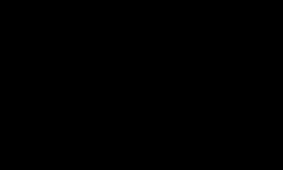
\includegraphics[width=85mm]{./imgs/im1.jpg}
\caption{\tiny{\Formular{Abraham Ortelius. {\slsc{Mapa da Islândia}} (séc. \protect\scalebox{.8}{XVI})}}}

\end{figure}

Ao mesmo tempo em que são autorais, sua existência como instrumento de
comunicação só é possível graças ao uso de um ``código'' (ou
``códigos'') comum. Informações diferentes, procedentes de instrumentos
separados, podem unificar"-se em uma só visão, porque suas ``inscrições''
possuem todas a mesma ``coerência ótica'', para usarmos a nomenclatura
do filósofo francês \index{Latour, Bruno}Bruno Latour (2004, p.~49).\footnote{\index{Latour, Bruno}Bruno Latour
  (2004, p.~40) assim explica sua nomenclatura: ``a informação não é um
  signo, e sim uma {\slsc{relação}} estabelecida entre dois lugares, o
  primeiro, que se torna uma periferia, e o segundo, que se torna um
  {\slsc{centro}}, sob a condição de que entre os dois circule um
  {\slsc{veículo}} que denominamos muitas vezes forma, mas que, para
  insistir em seu aspecto material, eu chamo de {\slsc{inscrição}}''.} Em
outras palavras, o mapa é uma linguagem e, para ser compreendido,
precisa fazer uso de um mesmo ``idioma visual'' entendido pelo autor e
pelo receptor. Uma vez que é produzido por alguém distante e dirigido
àqueles que não conhecem o território representado (mas têm que
acreditar nele), o mapa precisa fazer uso de um grande poder de
persuasão --- e persuasão é uma propriedade da linguagem que pode muito
bem ser confundida com sedução e beleza.

Se por muitos séculos aceitamos o mapa como simples redução gráfica do
mundo, hoje sabemos que sua confecção foi determinada por sistemas
dominantes de poder. Longe de ser um simples espelho da natureza, mapas
``redescrevem'' o mundo (como qualquer documento) em termos de relações
de poder e de práticas culturais, preferências e prioridades. O autor
escolhe o que vai incluir e o que vai omitir e, nesse processo de
decisão, está situado um complexo jogo de interesses. Por isso, não
podemos aceitar os mapas pelo seu valor de face e deveríamos
considerá"-los não apenas como representações do espaço, mas também como
espaços de representação (o geógrafo \index{Harvey, David}David Harvey alerta para a
necessidade de uma ``nova consciência cartográfica''). Devemos lembrar
que o processo de confecção dos mapas, desde sempre, nunca foi barato,
dependendo de instrumentos, pesquisas e deslocamentos dispendiosos.
Assim, apenas o Estado ou as grandes empresas puderam e podem criar
mapas sofisticados. Nesse sentido, o problema do mapa não é exatamente
como ele é feito, mas como é entendido e utilizado. Os mapas não são
inocentes.

Os mapas sempre estiveram ligados às disputas pela terra; a cartografia
lançou as bases legais para a própria noção de propriedade privada
baseada em privilégios de classe (\versal{HARVEY}, 2001, p.~22). Aquele que
desenha o mapa do terreno também desenha as fronteiras, as linhas
imaginárias e insere nomes sobre a superfície terrestre que determinam a
divisão de posse e os aspectos simbólicos do território --- uma questão
presente na disputa urbana, em pequena escala, mas também nas disputas
políticas e territoriais entre países.\footnote{Para prosseguir com os
  termos de \index{Latour, Bruno}Bruno Latour (2004, p.~51): ``o controle intelectual, o
  domínio erudito, não se exerce diretamente entre os fenômenos ---
  galáxias, vírus, economia, paisagens --- mais sim sobre as inscrições
  que lhe servem de veículo, sob a condição de circular continuamente, e
  nos dois sentidos, através de redes de transformações --- laboratórios,
  instrumentos, expedições, coleções''.} Segundo o geógrafo britânico
\index{Harley, John Brian}John Brian Harley, uma grande autoridade no assunto, o poder do mapa
equivale ao poder da palavra ou do livro como força de transformação. Os
cartógrafos ``fabricam poder'', criando um ``panóptico espacial''.
Afinal, onde traçar a linha do Tratado de Tordesilhas? Como separar a
Índia do Paquistão? A quem pertencem as Ilhas Malvinas? (ou seria melhor
dizer Falkland?) Como desenhar Israel e a Palestina?

Podemos dizer, portanto, que o conhecimento que o mapa carrega é
determinado por três instâncias: o cartógrafo, detentor do conhecimento
científico; a entidade (o Estado ou uma empresa), detentora do poder
econômico e nós, que recebemos o mapa sem poder questioná"-lo.

Mas como defini"-lo? Num artigo de 1996, o professor irlandês \index{Andrews, J. H.}J. H.
Andrews (1996) chegou a compilar 321 definições de mapa, sobretudo em
língua inglesa. Entre tantas palavras, três se destacam e aparecem com
mais frequência: ``superfície'', ``Terra'' e ``representação''. Assim,
se quisermos propor uma definição baseada na média, podemos dizer que
mapa é simplesmente a ``representação da superfície da Terra''. Na
prática, há duas definições importantes aceitas pelos estudiosos: para a
\emph{International Cartographic Association} mapa é a
``representação gráfica do espaço''; na obra \emph{History of
Cartography}, que vem sendo publicada desde 1987, sob a direção de \index{Harley, John Brian}J. B.
Harley e \index{Woodward, David}David Woodward (1987, p.~xvi), ``mapas são representações
gráficas que facilitam a compreensão espacial de coisas, conceitos,
condições, processos ou eventos no mundo humano''. Num sentido ainda
mais amplo, podemos recorrer à definição de cartografia proposta por
\index{Harvey, David}David Harvey (2001, p.~220, trad.~minha), segundo a qual ``a cartografia
trata de localizar, identificar e delimitar fenômenos e, assim, situar
eventos, processos e coisas numa moldura espacial coerente. Ela impõe
ordem espacial aos fenômenos''.

Se, por um lado, essas seriam as definições técnicas do objeto, o
significado do mapa e a atração que exerce podem ser melhor
compreendidos quando analisamos alguns mapas que tensionam os próprios
elementos que o definem. Há alguns mapas inverossímeis e ``inúteis''
propostos por autores da literatura e da filosofia que levam ao limite o
potencial poético e a limitação formal dos mapas. Um deles é o mapa
descrito neste trecho do romance \emph{Silvia e Bruno} (1889), de \index{Carroll, Lewis}Lewis Carroll (1997, p.~213):

\begin{quote}
--- Finalmente, tivemos a nossa grande ideia! Construímos o mapa do país
na escala de uma milha para uma milha!

--- E vocês o utilizaram muito? --- eu perguntei.

--- Ele nunca foi aberto, até hoje --- disse Mein Herr. --- Os fazendeiros
se opuseram, dizendo que o mapa cobriria todo o nosso território e
impediria a recepção da luz do sol! Por isso, atualmente, usamos o nosso
próprio território como mapa do país, e eu lhe asseguro que ele funciona
muito bem.
\end{quote}

Ser pequeno e maleável para atingir objetivos práticos de orientação é
da própria natureza do mapa e requisito para sua existência. A ideia de
um mapa em escala 1:1, que pudesse substituir o próprio território,
coloca em crise a relação entre objeto e sua representação provocando
uma espécie de colapso do signo linguístico, onde significante e
significado se anulam mutuamente.\footnote{Refiro"-me ao signo bipartido
  entre significante (a face visível, sensível, sonora --- o mapa) e
  significado (a coisa em si --- o território), conforme proposto por
  \index{Saussure, Ferdinand de}Ferdinand de Saussure (1975).} Esse paradoxo ficou mais conhecido
posteriormente através da célebre parábola \emph{Del rigor en la
ciencia} (1946), de \index{Borges, Jorge Luis}Jorge Luis Borges.\footnote{O texto foi publicado
  pela primeira vez na revista {\slsc{Los Anales de Buenos Aires}}, em
  março de 1946, como parte de um conjunto de textos chamado
  {\slsc{Museo}}, creditado a um certo B. \index{Lynch, Kevin}Lynch Davis, pseudônimo de
  \index{Borges, Jorge Luis}Borges e \index{Casares, Adolfo Bioy}Adolfo Bioy Casares. O texto, no entanto, traz a seguinte
  assinatura: ``Suárez Miranda: {\slsc{Viajes de varones prudentes}},
  Libro Cuarto, Cap. \scalebox{.8}{XLV}, Lérida, 1658''. Ver página \scalebox{.8}{XXXXX}.} O texto, de apenas um parágrafo, fala de um império onde a arte da cartografia
chegou a tal perfeição que ``los Colegios de Cartógrafos levantaron un
Mapa del Imperio, que tenía el tamaño del Imperio y coincidía
puntualmente con él''. Um mapa inútil, portanto, que as gerações
seguintes entregaram às ``Inclemencias del Sol y los Inviernos'' (2007,
v. \versal{II}, p.~265).

\index{Borges, Jorge Luis}Borges, por sua vez, parece ter se inspirado num mapa descrito pelo
filósofo idealista norte"-americano \index{Royce, Josiah}Josiah Royce (1855-1916). No conto
\emph{Magias parciales del ``Quijote''}, publicado no livro \emph{Otras
inquisiciones} (1952), \index{Borges, Jorge Luis}Borges cita (com modificações), um trecho do
autor, não sem antes dizer que ``las invenciones de la filosofia no son
menos fantásticas que las del arte'':

\begin{quote}
\index{Royce, Josiah}Josiah Royce, en el primer volumen de la obra \emph{The World and the
Individual} (1899), ha formulado la siguiente: ``Imaginemos que una
porción del suelo de Inglaterra ha sido nivelada perfectamente y que en
ella traza un cartógrafo un mapa de Inglaterra. La obra es perfecta; no
hay detalle del suelo de Inglaterra, por diminuto que sea, que no esté
registrado en el mapa; todo tiene ahí su correspondencia. Ese mapa, en
tal caso, debe contener un mapa del mapa, que debe contener un mapa del
mapa del mapa, y así hasta lo infinito'' (2007, v. \versal{II}, p.~56).
\end{quote}

Os três textos problematizam as consequências de confundirmos a
representação com a coisa representada. Embora tratem do mesmo paradoxo,
há interessantes diferenças entre eles. Em \index{Borges, Jorge Luis}Borges, o mapa é descartado
por sua própria inutilidade e seus fragmentos vão se despedaçando aos
poucos. No limite, se funde ao próprio território que representava e
começa a desaparecer. Já em \index{Carroll, Lewis}Carroll, diferentemente, não é o território
que sobrevive ao mapa, mas justamente o contrário. É o território que
toma o lugar do mapa, transformando"-se numa representação de si
mesmo. Aqui, é o mapa que sobrevive ao território, substituindo"-o. Em
\index{Royce, Josiah}Royce, nenhum dos dois é descartado, e multiplicam"-se infinitamente,
criando um jogo de espelhos, numa metáfora da loucura.

Isso nos leva a crer que, uma vez que algo encontra sua representação
perfeita, os dois lados se anulam, e será preciso optar por uma coisa ou
outra. \index{Borges, Jorge Luis}Borges opta pelo território, \index{Carroll, Lewis}Carroll pelo mapa e \index{Royce, Josiah}Royce tenta
inutilmente conciliar as duas coisas. Esse dilema fica mais claro quando
lemos outro texto de \index{Borges, Jorge Luis}Borges, chamado \emph{Parábola del palacio} (1960),
que pode ser entendido como um ``equivalente literário'' do problema do
mapa. O texto fala de um poeta que, num curtíssimo poema (``hay quien
entende que constaba de un verso; otros, de una sola palabra'') foi
capaz de retratar o palácio imperial por inteiro, em toda suas minúcias,
``con cada ilustre porcelana y cada dibujo en cada porcelana y las
penumbras y las luces de los crepúsculos y cada instante desdichado o
feliz de las gloriosas dinastías de mortales, de dioses y de dragones
que habitaron en él desde el interminable pasado'', e é imediatamente
morto pelo imperador diante de tamanha ousadia. \index{Borges, Jorge Luis}Borges (2007, v. \versal{II}, p.~214) sugere que bastou o poeta recitar o poema, para o palácio
desaparecer (``me has arrebatado el palacio'', lamenta o imperador),
pois ``en el mundo no puede haber dos cosas iguales''.

Com a perplexidade causada diante de representações de tal
escala, \index{Borges, Jorge Luis}Borges, \index{Carroll, Lewis}Carroll e \index{Royce, Josiah}Royce ilustram com perfeição o dilema
filosófico condensado na conhecida advertência do cientista e filósofo
polonês \index{Korzybski, Alfred}Alfred Korzybski: ``o mapa não é o território''. Embora seja
claro que não se deva confundir uma coisa com a outra, isso sempre
aconteceu e, segundo pensadores contemporâneos, acontece cada vez mais.

No mundo dominado pela tecnologia e pela onipresença das imagens, essa
questão se torna cada vez mais relevante. Um exemplo é visto nas salas
dos grandes museus espalhados pelo mundo. Muitas vezes o visitante, ao
perceber a presença de uma pintura conhecida, empunha a câmera
fotográfica e, num ato contínuo, fotografa a obra (muitas vezes com o
cuidado de enquadrar perfeitamente) e deixa a sala do museu sem
realmente \emph{ver} a obra com os próprios olhos. Ou seja, ele utiliza
o único momento que teve para olhar o quadro, com suas cores originais e
texturas (a oportunidade para desfrutar de sua ``aura'' como diria
\index{Benjamin, Walter}Walter Benjamin), para substituir essa experiência única pelo ato
fotográfico. O resultado será uma representação pobre e defeituosa do
quadro cuja função seria, ironicamente, provar que o visitante conheceu
a obra. Aqui, a representação substitui a coisa (ou a experiência) que
deveria apenas representar. No limite, não precisaremos mais da
coisa.\footnote{Na religião muitas vezes a imagem do personagem (ou o
  objeto onde essa imagem é materializada) é tão importante quanto o
  próprio personagem e se torna objeto de veneração, como no caso dos
  ícones da igreja bizantina. Daí o movimento iconoclasta dos séculos
  \scalebox{.8}{VIII} e \scalebox{.8}{IX}, que tentou proibir o culto desses objetos, acusando seus
  adoradores de ``idolatria'' que, na definição de \index{Levi-Strauss, Claude@Lévi-Strauss, Claude}Lévi"-Strauss é ``a
  presença pessoal do deus no seu simulacro''. Ver \scalebox{.8}{LÉVI"-STRAUSS}, Claude.
  {\slsc{Tristes Trópicos}}. São Paulo, Companhia das Letras, 1998, p.~427.}

\index{Baudrillard, Jean}Baudrillard enxergou nessa situação
uma característica importante da pós"-modernidade. Em \emph{Simulacros e
simulações} (1981), defende que chegamos a um ponto de saturação visual
onde já é possível \emph{substituir} a realidade por sua representação. Com
isso, a relação da representação com a coisa representada sofre um
grande abalo, relativizando o próprio encanto da abstração:

\begin{quote}
Hoje a abstração já não é a do mapa, do duplo, do espelho ou do
conceito. A simulação já não é a simulação de um território, de um ser
referencial, de uma substância. É a geração pelos modelos de um real sem
origem nem realidade: hiper"-real. O território já não precede o mapa,
nem lhe sobrevive. É agora o mapa que precede o território (\versal{BAUDRILLARD},
1981, p.~8).
\end{quote}

As imagens se tornam superfícies visuais sem conteúdo que, por isso,
adquirem ``intensidade espectral, vazia de sentido''.\footnote{Ver
  \index{Fabbrini, Ricardo}\scalebox{.8}{FABBRINI}, Ricardo Nascimento. ``Estética e crítica da arte em
  \index{Lyotard, Jean-François}Jean"-François Lyotard''. {\slsc{O Que nos Faz Pensar: Cadernos do Departamento
  de Filosofia da \scalebox{.8}{PUC}-Rio}}, Rio de Janeiro, v. 26, n. 40, pp.~47-77, 2017.}
Como pura superficialidade, são desprovidas de segredo e de mistério.
São o que o \index{Baudrillard, Jean}Baudrillard chama de \emph{simulacros}, imitações que nada \label{simulacros}
escondem pois não há nada por detrás delas a ser escondido.

Para \index{Baudrillard, Jean}Baudrillard, esses modelos de representação se distanciam tanto do
real que este se torna, paradoxalmente, uma utopia a ser alcançada. A
representação fotográfica contemporânea, por exemplo, com suas câmeras e
telas de alta definição, se torna tão sofisticada, ``hiper"-real'', que \label{hiperreal}
parece ``mais real do que o real'', relegando nossa experiência vivida e
imediata a uma condição subalterna e defeituosa. Diante disso --- que o
professor \index{Fabbrini, Ricardo}Ricardo Fabbrini (2016, p.~67) chama de ``déficit ontológico'' ---, não resta \label{deficit}
alternativa a não ser fotografar mais e mais, num processo inútil e
desesperador de busca de um real que talvez tenha deixado de existir.
Estaríamos, portanto, no campo das imagens, diante de uma lenta ``morte
do real'', que vai implicar também na ``morte de certa ideia de cultura,
vinculada ao erotismo e à sedução, ao sagrado e ao segredo''.\footnote{Ver página~\pageref{compulsiva}.}

Agora, os recentes avanços da cartografia por satélite e veículos não
tripulados, cujas imagens alimentam as plataformas digitais como o
\emph{Google Earth} e \emph{Google Street View}, lançaram um novo
paradigma para a relação mapa"-território. A capacidade de aproximação e
imersão nos mapas, as vistas aéreas e a modelagem 3D dos edifícios,
começam a apagar a distância que separa os lugares reais de suas
representações visuais, colocando em xeque as noções até então
indisputadas de original, verdadeiro e referente.

Essa situação foi ironicamente ilustrada pelo artista alemão \index{Bartholl, Aram}Aram
Bartholl na série \emph{Map} (2006-2012), em que instala ``pins''
gigantes em lugares públicos, como se fincasse um alfinete colorido
diretamente na superfície da Terra. Com esse gesto simples, e
utilizando"-se da iconografia própria das plataformas digitais, o artista
eleva o marcador virtual de local à categoria de monumento ao mesmo
tempo em que transforma o mundo num grande mapa à maneira de \index{Carroll, Lewis}Carroll e
\index{Borges, Jorge Luis}Borges. O antigo dilema mapa/território pode ser atualizado e entendido
agora na chave real/virtual. De forma análoga, no premiado romance
\emph{O mapa e o território} (2010), o escritor francês \index{Houellebecq, Michel}Michel
Houellebecq tensiona ainda mais (e também com ironia) esse dilema. O
personagem principal do livro é um artista contemporâneo que alcança o
sucesso com um trabalho onde fotografa e amplia as páginas dos mapas
rodoviários Michelin. O título da exposição de suas fotografias é ``O
mapa é mais interessante que o território'' (2012, p.~73).

\begin{figure}[!ht]

\centering
 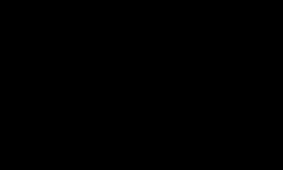
\includegraphics[width=85mm]{./imgs/im1.jpg}
\caption{\tiny{\Formular{\index{Bartholl, Aram}Aram Bartholl. {\slsc{Map}}, Arles (2011)}}}

\end{figure}

Outro mapa absurdo de \index{Carroll, Lewis}Carroll é o famoso ``mapa de Bellman'', do poema
\emph{nonsense} \emph{A caçada do Snark} (1876) (trad.~minha): \label{bellman}

\begin{verse}
Ele nos trouxe um grande mapa \qb{}representando o mar,\\
Sem o menor vestígio de terra:\\
E a tripulação ficou muito contente \qb{}quando perceberam\\
Que era um mapa que todos entendiam.\\[5pt]
``De que servem os Polos e Equadores \qb{}de \index{Mercator, Gerardo}Mercator,\\
Trópicos, Zonas e Meridianos?''\\
Assim gritava o capitão Bellman: e a \qb{}tripulação respondia,\\
``São apenas signos convencionais!''\\[5pt]
``Outros mapas têm formas, com suas \qb{}ilhas e cabos!\\
Mas gostaríamos de agradecer nosso \qb{}bravo capitão''\\
(Gritava a tripulação) ``pois ele nos \qb{}trouxe o melhor ---\\
Uma perfeita e absoluta folha em \qb{}branco!''\footnote{``He had brought a
  large map representing the sea,/ Without the least vestige of land:/
  And the crew were much pleased when they found it to be/ A map they
  could all understand.// `What's the good of Mercator's North Poles
  and Equators,/ Tropics, Zones, and Meridian Lines?'/ So the Bellman
  would cry: and the crew would reply,/ `They are merely conventional
  signs!'// `Other maps are such shapes, with their islands and capes!/
  But we've got our brave Captain to thank'/ (So the crew would
  protest) `hat he's bought us the best ---/ A perfect and absolute
  blank!'" (\scalebox{.8}{CARROLL}, 1962).}
\end{verse}

Aqui estamos diante de outro tipo de inutilidade, igualmente intrigante.
O mapa de Bellman nos lembra com extrema simplicidade que todo mapa é um
fragmento autoritário da superfície da Terra, um recorte. Em geral são
quadrados ou retangulares, formatos que em nada se assemelham às
irregularidades dos oceanos, países e continentes. Além disso, há o
clássico problema cartográfico da \emph{projeção}, ou seja, da
representação do globo terrestre numa superfície plana --- o planisfério
---, que invariavelmente distorce a superfície da Terra.

Mas a vocação fragmentada do mapa permite que ele possa ser entendido
como uma peça de um quebra"-cabeça gigantesco, aumentando ainda mais
nossa imaginação especulativa: onde começa? onde termina? o que há ao
lado? Esse aspecto fragmentado mas, por isso mesmo, suscetível à
montagem infinita foi celebrado pelos filósofos \index{Deleuze, Gilles}Gilles Deleuze e \index{Guattari, Félix}Félix Guattari (2011, p.~30), que enxergaram no mapa uma estrutura
\emph{rizomática}, voltada para a experimentação:

\begin{quote}
O mapa é aberto, e conectável em todas as suas dimensões, desmontável,
reversível, suscetível de receber modificações constantemente. Ele pode
ser rasgado, revertido, adaptar"-se a montagens de qualquer natureza, ser
preparado por um indivíduo, um grupo, uma formação social. Pode"-se
desenhá"-lo numa parede, concebê"-lo como obra de arte, construí"-lo como
uma ação política ou como uma meditação.
\end{quote}

O mapa de Bellman representa o \emph{meio} do oceano e, para
compreendê"-lo, podemos fazer novamente uso do conceito de \emph{rizoma}
proposto por \index{Deleuze, Gilles}Deleuze e Guattari. O rizoma, como vimos, é uma estrutura
sem começo nem fim cujo acesso se dá sempre pelo \emph{meio} pois, na
verdade, todas as suas mútltiplas entradas são \emph{meio}. Nesse
sentido, o meio não é o espaço entre uma e outra extremidade, ele é um
espaço entre dois outros \emph{meios}.

A forma esférica do globo terrestre contribui para essa sensação de
infinito. O planeta é um lugar que podemos percorrer infinitamente em
linha reta e onde, não importa a direção tomada, sempre se voltará ao
mesmo lugar. Qualquer fragmento da superfície terrestre, tal como
qualquer mapa, é meio.

O mapa vazio de Bellman, um mapa sem \emph{autor}, é o espaço das
possibilidades infinitas e libertário em sua essência e, por isso mesmo,
possui um potencial subversivo. O oceano de Bellman pode ser entendido
como a versão cartográfica de um \emph{terrain vague}, expressão cunhada
pelo arquiteto catalão \index{Solà-Morales, Ignasi de}Ignasi de Solà"-Morales (2002, p.~126) para descrever espaços vazios e indeterminados mas, por isso
mesmo, cheios de possibilidades imaginativas. Ou como o \emph{espaço}
\emph{liso} por excelência. Para \index{Deleuze, Gilles}Deleuze e Guattari, o oceano (assim
como o deserto e a estepe) é o espaço \emph{liso} por excelência (ao
contrário da cidade, que é o espaço \emph{estriado} por excelência), é
espaço do \emph{nômade}, esse sujeito incontrolável e imprevisível que,
justamente por isso, desafia o poder do Estado.

\begin{figure}[!ht]

\centering
 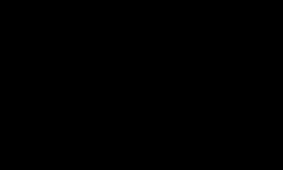
\includegraphics[width=85mm]{./imgs/im1.jpg}
\caption{\tiny{\Formular{Henry Holiday. {\slsc{Ocean"-Chart}} (1876). Ilustração para a\break primeira edição de {\slsc{A caçada do Snark}}, de \index{Carroll, Lewis}Lewis Carroll}}}

\end{figure}


O vazio do oceano coloca em xeque uma das funções mais importante dos
mapas: ordenar o território. Ao impor ordem ao território, o mapa também
busca impor controle e vigilância --- daí também a importância dos mapas
nas guerras e nas estratégias militares. Nesse sentido, o próprio ato de
desenhar um mapa implica uma atitude potencialmente repressora. \index{Deleuze, Gilles}Deleuze
e Guattari chamariam essa ordenação do território de \emph{estriamento}
do espaço liso, que pode a qualquer momento ser ``traçado e ocupado por
potências de \emph{organização} diabólicas'' (2012, p.~200). Assim,
apesar de celebrado por sua estrutura rizomática no que diz respeito à
sua forma física desmontável, o traçado do mapa esconde uma face
politicamente autoritária.

Podemos pensar que o mapa de Bellman é o mais preciso dos mapas na
medida em que representa com exatidão a superfície a que se propõe
representar, sem acrescentar nem omitir nada. Se, por um lado ele
aparenta uma inutilidade total, por outro é um mapa versátil, que pode
ser usado para representar qualquer oceano ou deserto --- e mesmo o
espaço sideral ---, em várias escalas. Ele cumpre com rigor tudo o que o
mapa deve ser ao representar com clareza uma parte da superfície
terrestre, ao ordenar o mundo e aguçar nossa imaginação ao mesmo tempo
--- além de provocar diversas reflexões sobre a própria natureza dos
mapas.

Estamos, portanto, diante de quatro proposições: ``o mapa não é o
território'' (\index{Korzybski, Alfred}Korzybski), ``o mapa é o próprio território'' (\index{Carroll, Lewis}Carroll e
\index{Borges, Jorge Luis}Borges), ``o mapa precede o território'' (\index{Baudrillard, Jean}Baudrillard) e ``o mapa é mais
interessante que o território'' (\index{Houellebecq, Michel}Houellebecq) --- todas ao mesmo tempo
verdadeiras e inconclusivas. Com sua fina ironia, a ``folha em branco''
de \index{Carroll, Lewis}Carroll pode ser usada para exemplificar qualquer dessas proposições
acima --- todas elas desafiando o que sempre aceitamos como a definição
primeira desse fascinante objeto: ``o mapa representa o território''.

\chapter{\emph{Atlante} (1973), de Luigi Ghirri}

Na série \emph{Atlante} (1973), o fotógrafo italiano \index{Ghirri, Luigi}Luigi Ghirri
fotografa as páginas de seu atlas, mostrando detalhes e fragmentos dos
mapas ali impressos.\footnote{É exatamente o mesmo procedimento utilizado
  pelo artista Jed Martin, personagem principal do romance de Michel
  \index{Houellebecq, Michel}Houellebecq {\slsc{O mapa e o território}} (2010).} As fotografias
isolam partes dos mapas e dirigem nossa atenção aos diversos nomes,
símbolos, linhas e desenhos, entre tantas outras imagens enigmáticas,
muitas vezes sem permitir que identifiquemos os verdadeiros lugares. Ora
vemos uma estrada desértica em cujo centro se situa ``Atomic City'', ora
trata"-se de uma imagem totalmente azul apenas atravessada pela linha de
um meridiano e onde se lê a palavra ``oceano''. A série ainda mostra
cursos d'água, fronteiras, curvas de nível, marcações de latitude e
longitude, topônimos estranhos, coqueiros, ilhas e toda sorte de sinais
gráficos utilizados para compor os mapas.

\begin{figure}[!ht]

\centering
 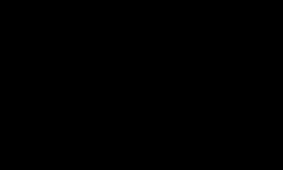
\includegraphics[width=85mm]{./imgs/im1.jpg}
\caption{\tiny{\index{Ghirri, Luigi}\Formular{Luigi Ghirri. Série {\slsc{Atlante}} (1973)}}}

\end{figure}

A natureza abstrata e figurativa dos mapas, apesar de sua pretensão
científica e da representação de lugares remotos, tem algo de íntimo e
poético. Esse símbolos e lugares desconhecidos provocam de maneira
lúdica e poderosa a mais criativa das capacidades humanas: a imaginação.
Quem já não se debruçou sobre um mapa a imaginar como seriam os lugares
ali representados através desses símbolos? O que há em Arkhangelsk,
Murmansk, Cluj e Qaqortoq? Quantas viagens já fizemos apenas examinando
mapas? Este trabalho de \index{Ghirri, Luigi}Ghirri pode ser entendido justamente como um
projeto de viagem imaginária, conceitual e poética através da descrição
abstrata do mundo gerada pela cartografia. Através dessas reproduções
realizadas por Ghirri, é possível vislumbrar os lugares visitados por
Ulisses, Robinson Crusoé, Phileas Fogg, e tantos personagens que
ativaram nossa imaginação desde a infância e cujas aventuras se
confundem com o próprio traçado de suas rotas sobre um mapa. A série de
\index{Ghirri, Luigi}Ghirri nos leva para uma verdadeira odisseia onde cada fotografia é uma
ilha ou uma aventura possível, como no texto de \index{Homero}Homero.

O prazer de observar um mapa também advém de sua eficiência como
organizador espacial. Ele nos mostra mais do que somos capazes de
abarcar com os próprios olhos e com nossa visão limitada, presa a um
corpo, condicionada a uma perspectiva individual. Com seu ponto de vista
aéreo e onisciente, nos permite ver a nós mesmos como um ponto minúsculo
em algum lugar, como se fossemos mais um de seus sinais gráficos. Assim,
ele é uma forma de entender o espaço onde estamos e contextualizar nosso
lugar no mundo.

O atlas é um objeto tão fascinante quanto o próprio mapa.\footnote{O
  termo tem origem na mitologia grega. Após ser derrotado pelos deuses,
  o titã Atlas foi condenado a sustentar o firmamento (e não o planeta,
  como muitos pensam) sobre os ombros. Ficou associado à cartografia
  após sua imagem ser usada para ilustrar coleções de mapas a partir do
  século \scalebox{.8}{XVI}. A palavra deu origem ainda a uma série de outras como
  Atlântico (oceano), Atlas (cadeia de montanhas), Atlântida (continente
  perdido) e atlante (coluna antropomórfica). Para \index{Didi-Huberman, Georges}Didi"-Huberman (2010a,
  p.~65), a figura do Atlas, com sua força, sabedoria e condenação
  representa o verdadeiro ``saber trágico'', cuja dor é proveniente do
  próprio peso do conhecimento. Seu rival mitológico seria Hércules mas,
  se Hércules encarna a potência ativa, Atlas encarna a potência imóvel
  da contemplacão.} E não é simplesmente uma coleção de mapas, mas um
objeto cultural com características próprias. O atlas é um artefato que
pretende reduzir o mundo ao tamanho de um livro. Constitui"-se numa
``forma visual do saber'', um instrumento original de leitura do mundo
que guarda mais semelhança com a enciclopédia e o dicionário do que com
o próprio mapa. Na definição do filósofo francês Georges \index{Didi-Huberman, Georges}Didi"-Huberman
(que se dedicou exaustivamente ao estudo do \emph{Atlas Mnemosyne}
{[}1927-1929{]}, de \index{Warburg, Aby}Aby Warburg), o atlas faz parte desses fascinantes
objetos que buscam classificar, ordenar e descrever as coisas do mundo;
é uma ``coleção de coisas singulares, em geral bastante heterogêneas,
cuja afinidade produz um saber estranho e infinito (nunca fechado):
samambaias, animais marinhos, ervilhas ou arquiteturas industriais,
etc., etc.'' (2010a, p.~284, trad.~minha).

O atlas não trata apenas da cartografia (há atlas de anatomia, atlas
históricos e outros) e é, antes de tudo, uma coleção de imagens. Cada
página apresenta uma ``lâmina'', que se conecta com as demais das mais
variadas formas. Pode"-se abrir um atlas em qualquer página, ir para
frente e para trás, como numa estrutura rizomática deleuziana. Aliás, é
muito difícil abrir um atlas apenas para ver a informação desejada, sem
se deixar levar pela curiosidade, que nos leva a outras páginas e outros
mundos. Frequentar um atlas é, como fez \index{Ghirri, Luigi}Ghirri, permitir uma
\emph{deriva} por suas imagens.

Não se pode esperar do mundo e, portanto, do atlas, uma forma
definitiva. Os atlas (como os dicionários e as enciclopédias) precisam
ser renovados para acompanhar as mudanças da geografia e os avanços da
tecnologia --- tarefa bastante ingrata no mundo contemporâneo,
caracterizado pela velocidade das transformações. Atlas antigos se
tornam cápsulas do tempo, fotografias congeladas de um mundo que já não
existe, como percebe \index{Didi-Huberman, Georges}Didi"-Huberman (2010b, p.~7): ``se o atlas aparece
como um trabalho incessante de recomposição do mundo, é, em primeiro
lugar, porque o mundo mesmo sofre decomposições constantes''. Como
instrumento do conhecimento, prossegue o filósofo francês (2010a, p.~15), o atlas ``desconstrói os ideais de unidade, de especificidade, de
pureza, de conhecimento integral. É uma ferramenta, não do esgotamento
lógico das possibilidades, mas da inesgotável abertura aos possíveis''

O atlas provoca nossa imaginação, essa poderosa e insubstituível arma do
conhecimento. Longe de ser um devaneio, uma fantasia, uma viagem
delirante sem sentido, a imaginação é uma faculdade humana que, como
afirma \index{Baudelaire, Charles}Baudelaire, percebe as ``relações íntimas e secretas das
coisas'', revelando seus significados ocultos e apontando soluções
originais para problemas aparentemente insolúveis. Justamente por sua
capacidade de associar, montar e colar imagens, a imaginação descobre
vínculos que a observação direta não é capaz de perceber.

No entanto, para\index{Ghirri, Luigi} Ghirri, o próprio atlas encerra uma contradição. É o
objeto que permite todas as viagens, mas não permite novas descobertas,
uma vez que mostra os lugares conhecidos e já visitados pelo homem. Nas
palavras do próprio Ghirri (2016, p.~39), o atlas ``cancela a própria
viagem, justamente porque todas as viagens possíveis já foram descritas
e todos os itinerários já foram traçados''. \index{Ghirri, Luigi}Ghirri, portanto, se utiliza
do potencial imaginativo do mapa ao mesmo tempo que constata sua
limitação como se o atlas prometesse todos esses mundos, mas na verdade
não entregasse nenhum.

Nesse sentido, a única viagem possível seria ``ao interior dos símbolos,
das imagens: na destruição da experiência direta'', como afirma o
próprio \index{Ghirri, Luigi}Ghirri (2016, p.~39).\footnote{Além de fotógrafo, \index{Ghirri, Luigi}Ghirri foi um
  importante pensador da fotografia contemporânea, tendo deixado vários
  escritos.} De que vale o deslocamento se temos ao nosso alcance todo o
mundo impresso num atlas? A ideia de ``destruição da experiência
direta'' se confunde com a substituição da experiência proporcionada
pelos meios de representação, sendo o mapa possivelmente o mais
fascinante de todos.

\chapter{Mapeamento como aventura}

Na pretensão de reproduzir o mundo, e utilizando"-se de seu próprio
encantamento, o mapa impõe uma visão sobre a superfície da Terra que,
por mais que aguce nossa imaginação, impede que tenhamos uma percepção
mais complexa e responsável do espaço. Como diz com simplicidade o
professor e artista \index{Wood, Denis}Denis Wood (1992, p.~1), uma série de interesses são
incorporados ao mapa na forma de presenças e ausências: ``cada mapa
mostra \emph{isto}\ldots{} e não \emph{aquilo}; cada mapa mostra desta
\emph{forma} e não de \emph{outra''}. O autor do mapa é aquele que
escolhe o que podemos e o que não podemos ver, uma arbitrariedade que
serve tanto para os mapas mais antigos quanto para as plataformas
atuais.

Esse perigo foi percebido por estudos mais recentes, como se o mapa
tivesse entrado numa era de suspeita, tendo ``perdido sua inocência''. A
exposição \emph{Cartes et figures de la terre} (1980), organizada pelo
Centro Georges Pompidou, em Paris (e seu rico catálogo) teve um papel
fundamental nessa nova abordagem para o estudo dos mapas, relativizando
a história da cartografia. Esses estudos deixaram claro que não podemos
mais estudar os mapas sem levarmos em conta os materiais de que são
feitos, o contexto cultural em que foram produzidos e seu apelo tanto ao
intelecto quanto à imaginação. Mais ainda, não podemos ignorar a
natureza igualmente libertadora e opressiva dos mapas.

Um dos grandes paradoxos do mundo contemporâneo é que o planeta nunca
foi tão bem mapeado (pensemos nas novas tecnologias) mas, ao mesmo
tempo, o homem nunca se sentiu tão desorientado espacialmente.\footnote{De forma semelhante, James Bridle (2018, p.~57) percebe que ``quanto mais ficamos obsessivos em computar o mundo, mais complexo e incognoscível ele parece''.} A
conhecida limitação dos mapas, a ilusão provocada por sua beleza e o
exercício de poder que engendra, parecem levar a uma conclusão
espantosa: os mapas estão limitando nossa capacidade de localização. Se
assim for, teremos apenas duas alternativas: ou tomamos conta do
processo de produção dos mapas, historicamente dominado pelas altas
instâncias do poder, ou será preciso descartá"-lo se quisermos saber onde
estamos.

Mas não apenas. Se, como vimos, Fredric \index{Jameson, Fredric}Jameson faz um chamado à
recuperação de nossa capacidade de situarmo"-nos relacionalmente nesse
espaço, está dizendo que esta é uma capacidade humana primordial que, em
algum momento da história, foi perdida. Com isso, abre"-se a pergunta:
terão os mapas, ao mostrarem um mundo pronto e sedutor, inibido nossa
própria capacidade natural de localização? Se esta capacidade de
localização está intimamente ligada à memorização do espaço e o mapa nos
entrega pronto justamente o que deveríamos memorizar, este alerta tem
fundamento. Nessa linha de raciocínio, teríamos que admitir que, quanto
mais usamos o mapa, mais perdemos nosso sentido de localização.

Esse paradoxo toma proporções gigantescas diante das novas tecnologias
de \emph{mapeamento} por satélite e dos mecanismos de geolocalização
embutidos nos dispositivos móveis como os celulares que carregamos no
bolso. Para \index{Virilio, Paul}Virilio (1993, p.~108), isto significará, em breve, um
estado de ``sedentariedade última, em que o controle do meio ambiente em
tempo real prevalecerá sobre a organização do espaço real do
território''.

Por exemplo, o \emph{Waze} é um navegador virtual que combina sofisticados
mapas e geolocalização por satélite (como \versal{GPS}), com uma série de dados
fornecidos pelos próprios usuários a fim de orientar o motorista na
cidade ou na estrada. Este dispositivo é capaz de planejar rotas, evitar
congestionamentos, alertar sobre a presença de radares, e indicar uma
série de serviços (além de exibir propaganda) ao motorista, ``em tempo
real''. Com ele, não é mais preciso saber de antemão o melhor caminho
entre dois pontos e o sentido das ruas; não é mais preciso perguntar às
pessoas sobre a localização onde se quer chegar. Não é mais preciso
prestar atenção no caminho e memorizá"-lo. O \emph{Waze} (e outros
``aplicativos'' similares) conduz o motorista até seu destino, mas esse
motorista acaba se tornando incapaz de refazer o trajeto sem a ajuda do
dispositivo (que, inclusive ``fala'' a todo instante, antecipando
\emph{todos} os desvios do caminho, fazendo dos trajetos uma espécie de
tortura, onde não há lugar para o silêncio que poderia ser utilizado
para a reflexão e memorização do espaço). É como se o indivíduo delegasse
a memória ao aplicativo, tornando"-se refém do aparelho que carrega consigo.
Embora facilite o
deslocamento, cria uma dependência que destrói nossa capacidade de
localização. Se o dispositivo falha, estamos perdidos como um barco à deriva no meio do oceano de Bellman.

\begin{figure}[!ht]

\centering
 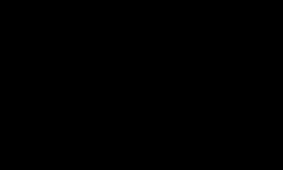
\includegraphics[width=85mm]{./imgs/im1.jpg}
\caption{\tiny{\Formular{Tela do aplicativo {\slsc{Waze}}}}}

\end{figure}

Para aprimorarmos nossa capacidade de localização autônoma vamos
precisar exercitar nossa capacidade de \emph{mapear} o espaço. O
mapeamento é um método eficaz e primitivo de leitura do espaço, uma
prática que está na origem do mapa, intimamente ligado à nossa
capacidade de memorização espacial conforme o deslocamento do corpo ---
comum a muitos animais, como vimos no capítulo anterior. É uma técnica
natural de iluminação gradual e lenta do território desconhecido, que
vai se revelando à medida do deslocamento. É o oposto de um salto no
escuro.

As diferenças entre mapa e mapeamento podem inclusive colocar os dois
termos em campos diametralmente opostos. O mapa é um objeto, o
mapeamento é uma prática. O mapa está ligado à imagem, ao espaço, ao ver
e à simultaneidade, enquanto o mapeamento está relacionado ao percurso,
ao tempo, ao ir e à temporalidade. O mapeamento implica movimento do
corpo; o mapa apresenta o espaço em sua totalidade, de uma só vez. O
mapa atiça nossa visão; o mapeamento exige poder de visualização. Se
quiséssemos transpor essas práticas para o mundo da arte, veríamos que o
mapa está mais próximo da pintura e da fotografia (artes do espaço)
enquanto o mapeamento se relaciona com a poesia, a música e a dança
(artes do tempo).

Com base nesses antagonismos, podemos propor a seguinte tabela:

\begin{table}[!htbp]
\begin{tabular}{ll}
\textbf{Mapa}         & \textbf{Mapeamento} \\
objeto                & prática             \\
material              & imaterial           \\
estático              & movimento           \\
registro              & memória             \\
observação            & experiência         \\
imagem                & percurso            \\
ver                   & ir                  \\
sobrevoo              & imersão             \\
óptico                & tátil (ou háptico)  \\
simultaneidade        & sequencialidade     \\
visão                 & visualização        \\
olho                  & corpo               \\
sincronia             & diacronia           \\
aceleração            & retardamento        \\
pintura, fotografia   & música, dança       \\
bidimensional         & tridimensional      \\
imediaticidade        & temporalidade       \\
objetividade          & subjetividade       \\
afastamento           & proximidade         \\
\end{tabular}
\end{table}

\begin{table}[!htbp]
\begin{tabular}{ll}
superfície            & profundidade        \\
verticalidade         & horizontalidade     \\
fora                  & dentro              \\
céu                   & chão                \\
Ícaro                 & \index{Dedalo@Dédalo}Dédalo              \\
divindade             & humanidade          \\
razão                 & emoção              \\
sedução               & esforço             \\
passividade           & atividade           \\
observação utilitária & leitura crítica    
\end{tabular}
\end{table}

Lembremos que o mapa é um objeto que nos apresenta o espaço de uma só
vez, onde todos os lugares se colocam simultaneamente diante de nossos
olhos, não havendo, portanto, propriamente uma leitura do espaço que se
desenvolva no tempo, com possibilidades de paradas, acelerações e
retardamentos (diferentemente do atlas, que possibilita uma leitura
temporal na medida em que percorremos suas páginas). Some"-se a isso um
mundo caracterizado pela tecnologia móvel e pela crescente velocidade
das experiências e temos como resultado uma atrofia de nossa capacidade
de memorização. Para o escritor tcheco \index{Kundera, Milan}Milan Kundera (2011, p.~30) há um
``elo secreto'' entre lentidão e memória, entre velocidade e
esquecimento, onde ``o grau da lentidão é diretamente proporcional à
intensidade da memória; o grau da velocidade é diretamente
proporcional à intensidade do esquecimento''.\footnote{Há quem veja na
  ideia de esquecimento uma virtude. No conto {\slsc{El Zahir}} (1949)
  \index{Borges, Jorge Luis}Jorge Luis Borges alerta para o perigo daquilo que é ``inesquecível''.
  O Zahir é uma moeda mística da qual não se pode esquecer e, por isso,
  vai ocupando todo o pensamento, não restando lugar para nenhum outro:
  ``ya no percibiré el universo, percibiré el Zahir'' (2007, v. \scalebox{.8}{II}, p.~715). No mesmo sentido, para \index{Virilio, Paul}Virilio (1993, p.~81), o esquecimento é
  condição de possibilidade do próprio imaginário.}

Portanto, a diferença mais importante é que o mapeamento induz a uma
\emph{leitura crítica} do espaço, diferente do mapa, que sugere a
\emph{observação utilitária} desse mesmo espaço. Sendo assim é uma capacidade natural cujo potencial pode ser tanto opressor quanto libertário. Pode ser usado como estratégia militar ou de caça, ligado à ideia de controle e vigilância do território, por exemplo. Mas também, na medida em que faz do sujeito autor de seu próprio espaço, pode ser uma atividade de emancipação do sujeito e, consequentemente, de transformação do meio e da sociedade.

A rigor, o mapeamento precede o mapa da mesma forma que o deslocamento
precede a medição do espaço. Para compreender melhor essas relações,
podemos recorrer a esta bela imagem de \index{Certeau, Michel de}Michel de Certeau (1998, p.~206):

\begin{quote}
Entre os séculos \versal{XV} e \versal{XVII}, o mapa ganha autonomia. Sem dúvida, a
proliferação das figuras ``narrativas'' que o povoam durante muito tempo
(navios, animais e personagens de todo o tipo) tem ainda por função
indicar as operações --- de viagem, guerreiras, construtoras, políticas
ou comerciais --- que possibilitam a fabricação de um plano geográfico.
Bem longe de serem ``ilustrações'', glosas icônicas do texto, essas
figurações, como fragmentos de relatos, assinalam no mapa as operações
históricas de que resulta. Assim a caravela pintada no mar fala da
expedição marítima que permitiu a representação das costas.
\end{quote}

\index{Certeau, Michel de}Certeau nos lembra que na origem do mapa está o percurso, a viagem.
Antes de se realizar numa folha de papel que simula a visão de fora,
alguém percorreu o espaço e registrou uma sucessão de etapas. Há,
portanto, uma relação indissociável entre o itinerário (uma série
discursiva de operações) e o mapa (uma descrição redutora totalizante
das observações), isto é, entre duas linguagens simbólicas e
antropológicas do espaço (\versal{CERTEAU}, 1998, p.~204).

O percurso e o deslocamento que antecedem o mapa mostram que, por trás
dele, há uma ideia narrativa, temporal, que muitas vezes passa
despercebida. E essa narrativa, por mais científica e objetiva que
deseje ser, está sempre sujeita às subjetividades humanas. Dessa forma,
qualquer relato de uma viagem ou de uma caminhada (o mais simples dos
deslocamentos humanos) é descrição \emph{e} construção do espaço, um ato
perceptivo \emph{e} criativo; leitura \emph{e} escrita do território ao
mesmo tempo, como nos mostra o professor italiano \index{Careri, Francesco}Francesco Careri,
autor do livro \emph{Walkscapes: o caminhar como prática
estética}, obra que investiga diversos significados críticos do ato de
caminhar.

Na literatura, uma obra que ilustra esse potencial poético e narrativo
do mapeamento é \emph{Os autonautas da cosmopista, ou, Uma viagem
atemporal Paris"-Marselha} (1983), de \index{Cortázar, Julio e Dunlop, Carol}Julio Cortázar e Carol Dunlop. O
casal decide fazer o trajeto entre as duas cidades seguindo algumas
regras:

\begin{enumerate}
\item[1.] Cumprir o trajeto de Paris a Marselha sem sair nem uma vez da
estrada.

\item[2.] Explorar cada uma das paradas, duas por dia, passando sempre a noite
na segunda, sem exceção.

\item[3.] Realizar levantamentos científicos de cada parada, tomando nota de
todas as observações pertinentes.

\item[4.] Inspirando"-se nos relatos de viagem dos grandes exploradores do
passado, escrever um livro da expedição (modalidades a determinar)
(2013, p.~38).
\end{enumerate}

O mapeamento aqui tem motivação afetiva. A viagem de seiscentos
quilômetros, que normalmente se faz em algumas horas, foi completada em
mais de trinta dias. O casal parte de um protocolo, e transforma (com
humor) a viagem numa ``exploração científica'', criando um jogo, um
mapeamento ``sem sentido'' como ciência, mas afetuoso e divertido. A
bordo de uma \emph{kombi} (que eles apelidaram de \emph{Fafnir}, como o
dragão) param para comer ou dormir a cada poucos minutos, em lugares
aparentemente desinteressantes como restaurantes e pequenos hotéis de
beira de estrada --- uma expedição em busca de uma ``conquista do
inútil'',\footnote{Título de um livro do cineasta \index{Herzog, Werner}Werner Herzog, onde
  relata os bastidores da filmagem de {\slsc{Fitzcarraldo}} (1982).}
fazendo do ato de desperdiçar tempo um projeto criativo e uma crítica à
produtividade constante que o mundo nos exige.

Se o mapa oferece o conforto de ter o mundo entre as mãos, o mapeamento
é percurso e viagem --- portanto é aventura, descoberta e perigo (aspecto
exaustivamente explorado pela literatura, bastando citar a Odisseia, de
\index{Homero}Homero, modelo de todas as aventuras). A esse respeito, \index{Foucault, Michel}Michel Foucault
nos oferece uma belíssima metáfora do barco, este instrumento de
mapeamento por excelência, como ``reserva de imaginação'':

\begin{quote}
se considerarmos que o barco, o grande barco do século \versal{XIX}, é um pedaço
de espaço flutuante, lugar sem lugar, com vida própria, fechado em si,
livre em certo sentido, mas fatalmente ligado ao infinito do mar que, de
porto em porto, de zona em zona, de costa a costa, vai até as colônias
procurar o que de mais precioso elas escondem naqueles jardins orientais
que evocávamos há pouco, compreenderemos porque o barco foi, para nossa
civilização --- pelo menos desde o século \versal{XVI} --- ao mesmo tempo, o maior
instrumento econômico e nossa maior reserva de imaginação. O navio é a
heterotopia por excelência. Civilizações sem barcos são como crianças
cujos pais não tivessem uma grande cama na qual pudessem brincar; seus
sonhos então se desvanecem, a espionagem substitui a aventura, e a
truculência dos policiais, a beleza ensolarada dos corsários''
(\index{Foucault, Michel}\versal{FOUCAULT}, 2013, p.~30).
\end{quote}

Viajar é sempre uma busca. A viagem pode ter motivação econômica (as
``Grandes Navegações''), religiosa (as Cruzadas), diplomática (a viagem
de \index{Polo, Marco}Marco Polo), científica (a viagem do Beagle), educacional (o ``Grand
Tour''); pode ser um retorno (a Odisseia) ou uma fuga (a viagem de D.
João \versal{VI} ao Brasil), mas sempre implica a ideia de \emph{experiência}. O
pedagogo \index{Larrosa, Jorge}Jorge Larrosa (2002, p.~25) nos ensina que o radical da palavra
\emph{experiência} é \emph{periri}, que se encontra também em
\emph{periculum} (perigo). A raiz indo"-europeia é \emph{per}, que se
relaciona com a ideia de ``travessia'' e de ``prova''. Em grego há
numerosos derivados dessa raiz que marcam a travessia, o percorrido, a
passagem: \emph{peirô} (atravessar), \emph{pera} (mais além),
\emph{peraô} (passar através), \emph{perainô} (ir até o fim),
\emph{peras} (limite). Mesmo a palavra ``pirata'' pertence à mesma
família. Em alemão, experiência é \emph{Erfahrung}, que contém
\emph{fahren} (viajar). E do antigo alto"-alemão \emph{fara} também
deriva \emph{Gefahr} (perigo), e \emph{gefährden} (pôr em perigo).
Portanto, experiência e perigo são palavras que andam juntas, mostrando
que a própria ideia de conhecimento e instrução implica também
esforço, sacrifício e risco.

Mas a verdadeira experiência é cada vez mais rara. Vivemos num mundo
onde frequentemente confundimos informação com experiência, sendo que o
excesso de informação a que somos submetidos é, na verdade, a antítese
da experiência. Se temos acesso à informação (pensam alguns) não há razão para a busca do conhecimento pela experiência com todo o risco que implica. Larossa afirma que o ``sujeito da experiência'' é aquele
que busca e que está disponível ao mesmo tempo, aberto aos ocasos da
vida; que permite espaços vazios para serem preenchidos pela surpresa. É
um sujeito que se expõe, cuja passividade é uma atitude afirmativa.
Experiência não é o que o sujeito \emph{faz}, mas aquilo que permite que
lhe aconteça.

Portanto, se na raiz do mapeamento está a ideia de experiência, teremos
que enfrentar os perigos do percurso e, ao mesmo tempo, estar
disponíveis para as surpresas, algo que não vai acontecer atrás de uma
tela por onde chegam ``informações''.

\chapter{Pré-cartografias}

É interessante notar que em seu livro \emph{A imagem da cidade} (1960),
\index{Lynch, Kevin}Kevin Lynch não tenha se debruçado sobre o papel e o significado do mapa
no desenvolvimento de seu conceito de \emph{legibilidade} da cidade.
Lynch por vezes usa o mapa como instrumento de seu método de trabalho,
sobretudo quando entrevista pessoas na rua. Mas, no fundo, a proposta de
\index{Lynch, Kevin}Lynch, preocupado com a percepção fenomenológica da cidade, precisa
\emph{excluir} o mapa. Ele percebe justamente o prejuízo da nossa
capacidade de mapeamento que o mapa provoca e insiste na imagem da
cidade vista por seus cidadãos, ao nível da rua. Uma rua ou uma praça
podem adquirir forma e sentido bastante diferentes se as percebemos
vindo desta ou daquela rua; já o mapa apresenta a rua e a praça da mesma
forma para todos. Em sua pesquisa, \index{Lynch, Kevin}Lynch está a todo momento provocando
o cidadão a \emph{narrar} sua experiência na cidade, a relatar sua
percepção com base nos trajetos e itinerários --- um exercício ainda
pré"-cartográfico que enfatiza a importância da cidade como experiência
temporal, onde ``a cada instante existe mais do que a vista alcança''
(1980, p.~11). \index{Lynch, Kevin}Lynch percebe que o mapeamento é mais importante que o
mapa e é uma condição para que ele exista --- uma relação muitas vezes
invertida (é este aspecto de seu livro que atraiu a atenção de Fredric
\index{Jameson, Fredric}Jameson em sua proposta de mapeamento cognitivo, como vimos). Um dos
métodos de \index{Lynch, Kevin}Lynch para avaliar a percepção dos cidadãos sobre a cidade
era a entrevista. E uma das perguntas que fazia aos entrevistados revela
bastante sobre seu interesse:

\begin{quote}
Dê"-nos, por favor, uma descrição completa e explícita das direções por
si usadas, quando vem do trabalho para casa. Faça a descrição de si
próprio quando faz este percurso e descreva a sequência do que pode ver,
cheirar e ouvir ao longo do caminho, incluindo o que é para si
importante e as indicações de que um estranho necessitaria para tomar as
mesmas decisões na escolha do caminho que por si são tomadas. Estamos
interessados na descrição física das coisas. Não é importante lembrar"-se
do nome de ruas ou locais (1980, p.~154).
\end{quote}

Não por acaso algumas representações cartográficas antigas, como a
\emph{Tabula Peutingeriana} (conhecida através de uma cópia do século
\versal{XII} ou \versal{XIII} de um mapa romano do século \versal{IV}), desenhadas em longos
pergaminhos, eram extremamente compridas e muito mais preocupadas com as
rotas e itinerários do que com a representação fiel da superfície.
Nesses desenhos, chamados justamente \emph{itinerários} (do
latim \emph{itinerarium}), são assinaladas as cidades, vilas e albergues
a fim de orientar os viajantes; e representam uma espécie de elo perdido
entre a prática do mapeamento e os mapas como conhecemos.

\begin{figure}[!ht]

\centering
 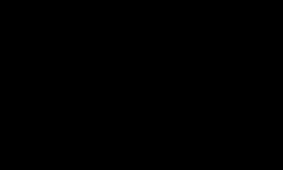
\includegraphics[width=85mm]{./imgs/im1.jpg}
\caption{\tiny{\Formular{Trecho da {\slsc{Tabula Peutingeriana}}\break (cópia de original romano do século \protect\scalebox{.8}{IV})}}}

\end{figure}

De forma semelhante, os códices astecas eram uma espécie de narrativa
pictórica pré"-cartográfica.\footnote{Esses documentos pictóricos são
  considerados as melhores fontes primárias sobre a cultura asteca,
  retratando hábitos, movimentos migratórios e a religiosidade desse povo.
  Os exemplares que chegaram aos nossos dias, salvo raras exceções,
  foram realizados após a chegada dos espanhóis, embora alguns sejam
  cópias de originais pré"-colombianos.} O \emph{Códex Xolotl} (séc.
\versal{XVI}), por exemplo, apresenta o vale central do México como um espaço
historicizado onde uma série de narrativas ocorrem de forma simultânea,
sobretudo ligadas às sucessões dinásticas dos povos que habitavam a
área. No \emph{Códex,} a representação do espaço tem pouco compromisso
com a verossimilhança. Lugares são superdimensionados, aproximados e
duplicados conforme sirvam à narrativa; distorções são relevadas em
função da dinâmica das realidades políticas. Há uma grande liberdade de
representação, apesar das codificações necessárias. São pré"-mapas em
movimento que carregam consigo a ideia temporal de \emph{narrativa}.

\begin{figure}[!ht]

\centering
 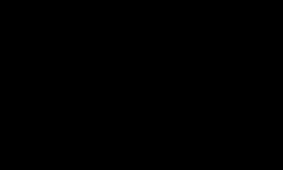
\includegraphics[width=85mm]{./imgs/im1.jpg}
\caption{\tiny{\Formular{{\slsc{Códex Xolotl}} (séc. \protect\scalebox{.8}{XVI})}}}

\end{figure}

Algumas dessas atividades pré"-cartográficas foram recuperadas em meados
do século \versal{XX} por estudiosos e artistas interessados no potencial
criativo da prática de mapeamento. Nesse contexto, o grupo situacionista
tem lugar de destaque. Sem querer abordar todas as implicações culturais
desse movimento, já bastante estudadas, uma análise do \emph{Guide
Psychogeographique de Paris: Discours Sur Les Passions D'Amour} --- o
primeiro mapa ``psicogeográfico'' proposto por \index{Debord, Guy}Guy Debord em 1956 ---
revela muito da compreensão espacial dos situacionistas. Concebido como
um folheto dobrável para ser distribuído aos turistas, o \emph{Guide} ---
invertendo a principal função de um mapa --- é um convite à desorientação
e à \emph{deriva}. A \emph{deriva} é de fato uma técnica subversiva de
apropriação do espaço urbano proposta pelos situacionistas que, através
de caminhadas sem destino, orientadas pelas ``solicitações do terreno''
e pelas possibilidades de encontro, dispara o poder revolucionário do
inconsciente --- uma proposta estética que se opõe à \emph{flânerie}
baudelairiana alienante e orientada pelo prazer fútil.

A Paris retratada se assemelha a um arquipélago onde troços da cidade
flutuam como num ambiente líquido em constante movimento, atraindo"-se ou
afastando"-se conforme critérios ``afetivos''. Trata"-se de uma geografia
instável que se transforma também no tempo, acompanhando o deslocamento
do observador. O mapa em si é a representação da variação perceptiva
daquele que caminha pelas ruas da cidade. As setas vermelhas tentam dar
conta das direções e intensidades desses deslocamentos possíveis entre
as ``ilhas''. Diferentemente de ruas e avenidas, não são ``traçados''
(como os bulevares \index{Haussmann, Georges-Eugène}haussmannianos), mas \emph{vetores} provisórios
\emph{entre} os pontos, como num portulano. Qualquer ponto pode ser
conectado a qualquer outro, não há hierarquias nem centralidade, como
num \emph{rizoma}.

\begin{figure}[!ht]

\centering
 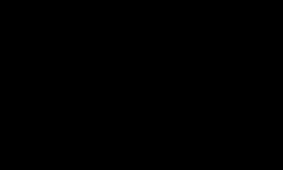
\includegraphics[width=85mm]{./imgs/im1.jpg}
\caption{\tiny{\Formular{\index{Debord, Guy}Guy Debord. {\slsc{Guide Psychogeographique de Paris:\break Discours Sur Les Passions D’Amour}} (1956)}}}

\end{figure}

Para \index{Debord, Guy}Debord, o mapa convencional é uma ferramenta enganosa que precisa
ser ``corrigida'' pela experiência subjetiva do cidadão. Para os
situacionistas, a paixão, o amor e o desejo (reparemos no título do
mapa) são elementos tão ou mais fundamentais para a leitura e construção
do espaço quanto a disposição geométrica das ruas e edifícios. Na
verdade, os elementos físicos da cidade apenas existem em relação aos
outros, mediados pela subjetividade do indivíduo. Na cidade
situacionista, a distância entre os pontos não é visual e metricamente
mensurável, mas \emph{sentida} por quem estiver disposto a perceber as
\emph{pulsões} que a cidade emana. Por isso, o mapa de \index{Debord, Guy}Debord está mais
preocupado com os espaços \emph{entre} os lugares, com os percursos e
trajetos. A cidade como um todo só existe como soma desses trajetos e
partes fragmentadas que devem ser unidas mentalmente pelo sujeito num
processo de reapropriação afetiva do território, provocando assim uma
reflexão crítica sobre o espaço urbano que poderíamos muito bem chamar
de ``mapeamento cognitivo''.

O mapa de \index{Debord, Guy}Debord, além das relações com os \emph{itinerários} romanos, é
bastante semelhante a um dos mais antigos ``mapas'' conhecidos pelo
homem. O chamado \emph{Mapa de Bedolina} é formado por um conjunto de
inscrições rupestres gravadas numa rocha do Vale Camonica, na Itália, ao
longo do primeiro milênio a.C.

\begin{figure}[!ht]

\centering
 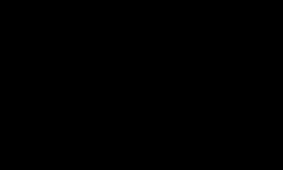
\includegraphics[width=85mm]{./imgs/im1.jpg}
\caption{\tiny{\Formular{Representação do {\slsc{Mapa de Bedolina}} (1 milênio a.C.)}}}

\end{figure}

Não se sabe ao certo se as inscrições de fato são um mapa como
concebemos, ou seja, uma visão planificada do território, visto de cima,
como parece.\footnote{Indisputadamente, o mapa mais antigo do mundo de
  que se tem conhecimento data do século \scalebox{.8}{V} ou \scalebox{.8}{IV} a.C. É o chamado
  {\slsc{Imago Mundi}}, uma tabuleta de argila descoberta nas ruínas de
  Sippar, antiga cidade na Mesopotâmia no atual Iraque. Representa o
  mundo na perspectiva dos povos da Babilônia, com o rio Eufrates e o
  próprio reino da Babilônia ocupando lugar de destaque. A peça, do
  tamanho de um telefone celular, encontra"-se no Museu Britânico. Ver
  \scalebox{.8}{BROTTON}, Jerry. {\slsc{Uma história do mundo em doze mapas.}} Rio de
  Janeiro: Zahar, 2014.} É difícil saber se esses povos da Idade do
Ferro tinham a capacidade de abstração exigida para a construção desse
tipo de mapa, embora seja tentador enxergar nessas inscrições a
representação de um território agrário. O \emph{Mapa de Bedolina} parece
apresentar todos os elementos que nos permitem reconhecê"-lo como um
mapa. As figuras geométricas parecem símbolos (representações de algo
que não está ali), os animais e figuras humanas sugerem algum tipo de
escala, as linhas parecem caminhos tortuosos (espaços de ir) que
conectam os espaços quadrados e delimitados (espaços de estar), como no
mapa de \index{Debord, Guy}Debord.

\begin{figure}[!ht]

\centering
 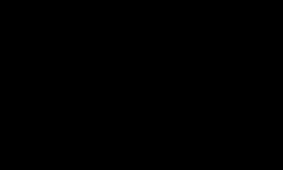
\includegraphics[width=85mm]{./imgs/im1.jpg}
\caption{\tiny{\Formular{Linhas de Nazca (entre 700 a.C. e 200 d.C.)}}}

\end{figure}

Mas, mesmo que o desenho seja outra coisa como um esquema de
distribuição de coisas, um sistema de contabilidade, o tabuleiro de um
jogo, a representação da divindade, um manual de instruções ou um
diagrama, não deixa de ser uma inscrição gráfica numa superfície
relativamente bidimensional que obedece a um princípio geometrizante do
espaço e que, portanto, situa ``eventos, processos e coisas numa moldura
espacial coerente'' e ``impõe ordem espacial aos fenômenos'', conforme a
definição de cartografia de \index{Harvey, David}David Harvey, como vimos.

Nessa linha de raciocínio, poderíamos incluir também outras inscrições
como os alinhamentos megalíticos de Carnac, na França, ou enormes
geóglifos, como as misteriosas linhas de Nazca, no Peru. Neste caso, é
tentador pensar (como nos mapas de \index{Carroll, Lewis}Carroll e \index{Borges, Jorge Luis}Borges) que a planície de
Nazca, onde o próprio solo desértico se tornou suporte das linhas e
desenhos geométricos, é um imenso mapa que representa a si mesmo.

\chapter{\emph{Costruzione legittima}}

Uma visão crítica do mapa necessariamente coloca em debate a questão do
ponto de vista. Tão importante quanto refletir sobre \emph{o que} é
aquilo que se vê, é perguntar"-se \emph{de onde} se vê aquilo.

A perspectiva linear é o sistema visual que dominou a forma de o \label{perspectiva}
Ocidente ver o mundo por mais de 500 anos e ainda exerce enorme
influência. É um sistema tão poderoso e sedutor (como os mapas) que
passamos a considerar essa proposição visual artificial como se fosse
natural e existisse desde sempre. No entanto, assim como os mapas, a
perspectiva é não só uma maneira de representar o mundo, mas também de
construí"-lo.

Elaborada (``descoberta'', ou ``inventada'') no Renascimento pelo
arquiteto \index{Brunelleschi, Filippo}Filippo Brunelleschi e descrita por \index{Alberti, Leon Battista}Leon Battista Alberti, a
perspectiva linear é um sistema criado para superar a dificuldade de se
representar realisticamente objetos tridimensionais numa superfície
bidimensional.\footnote{A perspectiva angular (elaborada por Euclides), a perspectiva axonométrica (utilizada em desenhos técnicos) e a perspectiva curvilínea são outros métodos de representação do espaço.} Para isso, usa princípios da matemática e da geometria
para criar uma ilusão de profundidade. \emph{Grosso modo}, um quadro que
obedece às regras da perspectiva é resultado da seção transversal plana
de uma pirâmide visual imaginária cujo vértice é o olho. Assim, quanto
mais distante está o objeto, menor ele é desenhado na superfície da
tela. A imagem resultante desse modelo matemático é a chamada
\emph{costruzione legittima}, que apresenta o mundo \emph{diante} de
nós, como se visto por uma janela aberta para a realidade. Nas palavras
do próprio \index{Alberti, Leon Battista}Alberti, em seu tratado \emph{Da pintura}, de 1435:

\begin{quote}
inicialmente, onde devo pintar, traço um quadrângulo de ângulos retos,
do tamanho que me agrade, o qual reputo ser uma janela aberta por onde
possa eu mirar o que aí será pintado, e aí determino de que tamanho me
agrada que sejam os homens na pintura (2014, p.~88).
\end{quote}

A perspectiva linear foi uma verdadeira revolução na história da arte ocidental
e, podemos dizer, na história da humanidade, determinando, em grande
medida, a forma como representamos e visualizamos o mundo até hoje. Em
que pese a perspectiva intuitiva de \index{Giotto}Giotto --- cuja pintura, por volta de
1300, já apresentava sofisticação espacial, profundidade e princípios de
tridimensionalidade ---, foi apenas a partir do século \versal{XV}, com a
introdução das regras da perspectiva linear, que a representação
pictórica europeia passou a caracterizar"-se por um ``naturalismo'' em
busca de uma ``verdade'' visual prometida pela nova técnica,
inicialmente colocada por \index{Alberti, Leon Battista}Alberti, mas depois aperfeiçoada pelos
próprios artistas.

Mas, como observa \index{Latour, Bruno}Bruno Latour (2015, p.~11), a qualidade principal
desse novo espaço visual não é exatamente sua pretensa ``objetividade'',
mas o que chama de ``consistência ótica''. A perspectiva, com sua
proposta de organização visual do espaço, acaba se tornando uma
verdadeira linguagem que usa regras, símbolos e formas invariáveis,
estabelecendo um padrão visual e aproximando indivíduos e culturas em
torno de uma ``gramática'' comum. Essa linguagem possibilitou uma
comunicação direta e visual de maneira impensável para a linguagem
verbal até então. Utilizando"-se de métodos e requisitos da ciência ao
apresentar propriedades de imutabilidade, consistência ótica, linguagem
homogênea e estabilidade geométrica, a perspectiva permite recriar uma
cena ou um quadro à distância, apenas informando as coordenadas
matemáticas do esquema, como um manual de instruções.\footnote{A
  {\slsc{Geografia}} (150 d.C.), de \index{Ptolomeu}Ptolomeu, foi o mais importante
  ``mapa'' da Antiguidade, tendo condicionado a concepção geográfica do
  mundo ocidental por mais de dois milênios. Na verdade, não se trata de
  um mapa desenhado, mas de um manuscrito que traz coordenadas
  geográficas de mais de oito mil lugares na Europa, África e Ásia, e
  uma espécie de manual que orienta a elaboração de mapas a partir
  desses dados. Foi esquecido e redescoberto apenas no século \scalebox{.8}{XIII}, e
  não se sabe se \index{Ptolomeu}Ptolomeu propriamente chegou a desenhar um mapa a
  partir dele.}

A formulação de uma lei comum para a natureza e para a forma artística
está na essência da perspectiva. Nesse sentido, como aponta o curador e
historiador \index{Ivins, William}William Ivins (1938, p.~9), ela pode ser considerada como
``um meio prático para garantir uma rigorosa relação métrica de duas
mãos (recíproca) entre as formas dos objetos definitivamente colocados
no espaço e suas representações pictóricas''. Em outras palavras,
aplicar as regras da perspectiva é uma forma de medir o mundo.

Certamente não se deve ao acaso ter sido elaborada por um arquiteto. Da
mesma forma que se alimenta de princípios científicos, a perspectiva
está também intimamente ligada ao desenvolvimento da arte. \index{Argan, Giulio Carlo}Giulio Carlo
Argan (1946, p.~96) argumenta que a própria ideia de beleza clássica
está relacionada com o conceito de harmonia e, portanto, de proporção.
Logo, se a perspectiva é o processo pelo qual se atinge a perfeita
proporção das formas, é também o processo pelo qual se chega à beleza
perfeita, associada à beleza clássica da Antiguidade. Esta era uma
grande busca do Renascimento, onde a perfeição e a fidelidade da cena
representada passaram a ser requisitos do belo. No limite, poderíamos
dizer que a beleza é simplesmente o resultado de regras matemáticas bem
aplicadas.

Acompanhando as transformações científicas, sociais e culturais da
época, o Renascimento significa a passagem de uma visão teocêntrica
medieval para uma visão antropocêntrica do mundo. As pinturas chapadas e
sem profundidade penduradas em igrejas mal iluminadas, os temas
religiosos fechados em si mesmos, os personagens retratados frontalmente
e dimensionados conforme sua importância, agora dão lugar a uma pintura
luminosa que apresenta o mundo ``real'', como visto através do buraco de
uma fechadura. Há um deslocamento do antigo ponto de vista dessa arte
medieval, obscura, difusa e dominada por uma interpretação mística e
religiosa da realidade para um ponto de vista claro de um novo homem
que, em breve, descobrirá novos mundos e abrirá horizontes por ``mares
nunca dantes navegados''.\footnote{Terceiro verso da primeira estrofe
  do Canto \scalebox{.8}{I} de {\slsc{Os Lusíadas}} (1572), de \index{Camões, Luís de}Luís de Camões.}

Justamente, uma característica fundamental da perspectiva clássica é a
existência de um observador imóvel, privilegiado, que enxerga o mundo a
partir de um único ponto de vista, considerado natural, científico e
objetivo. Agora, a percepção humana é o principal organizador do espaço
e, o homem, a própria medida do mundo. O olho passou a determinar o
tamanho e a distância relativa das coisas e qualquer observador colocado
naquele ponto veria as relações espaciais entre essas coisas exatamente
da mesma forma. Assim, a localização desse ponto passou a ser mais
importante do que o próprio sujeito que se encontrava nele. A pergunta
fundamental passou de ``quem'' para ``de que ponto no espaço?''. A
perspectiva, portanto, de fato pode ser considerada um triunfo da
afirmação do homem sobre a natureza (e sobre o divino), mas um triunfo
de um homem ideal ou genérico sobre um espaço geometrizado e impessoal.

O filósofo Henri \index{Lefebvre, Henri}Lefebvre em \emph{A produção do espaço} (1974), assim
resume a relação do espaço com sua representação, numa linha de
raciocínio que pode ser aplicada tanto à relação dos objetos com a
perspectiva linear, quanto à relação do mundo geográfico com os mapas:

\begin{quote}
O geométrico. É o espaço euclidiano considerado como ``absoluto'' pelo
pensamento filosófico, portanto há muito tempo o espaço de referência
(representação do espaço). Este espaço euclidiano se define por sua
\emph{isotopia} (sua homogeneidade), propriedade que garante seu uso
social e político. A redução do espaço"-natureza ao espaço euclidiano
homogêneo, em primeira instância e, em seguida, de todo o espaço social,
lhe confere um poder impressionante. Tanto mais que esta primeira
redução conduz facilmente a uma outra: a redução do tridimensional a
duas dimensões: o ``plano'', a folha de papel em branco, o desenho sobre
esta folha, os mapas, os grafismos e projeções (1974. p.~329, trad.
nossa).
\end{quote}

Portanto, apesar da afirmação da centralidade desse novo homem, a
perspectiva é uma abstração que ignora a percepção subjetiva do mundo.
Para que esse espaço racional, imutável e homogêneo funcione, é preciso
supor um observador igual a todos os outro, parado num chão estável,
olhando para frente em direção a um ponto de fuga situado próximo a um
horizonte reto, plano e artificial.\footnote{Os sonhos, por exemplo, apresentam uma proposta de compreensão do espaço completamente diferente. Num sonho, não há grande diferença entre ver o mundo e ver a si mesmo vendo o mundo. Há uma espécie de fusão do eu com esse mundo, algo que a perspectiva linear não seria capaz de representar.} Como observa a artista e
pesquisadora \index{Steyerl, Hito}Hito Steyerl (2012, p.~19, trad.~minha), ``ao mesmo tempo
em que dá autoridade ao sujeito ao colocá"-lo no ponto central da visão,
a perspectiva linear também mina a individualidade desse sujeito ao
submetê"-lo às supostas leis objetivas da representação''. O apelo
científico e pretensamente objetivo da perspectiva tenta estabelecer uma
relação com uma suposta ``verdade universal'' que acaba neutralizando a
busca das verdades individuais e conflitantes. Para \index{Steyerl, Hito}Steyerl, a
perspectiva linear se torna ``refém da verdade''.

Apesar da enorme aceitação dessa técnica de representação, alguns artistas acabaram relativizando o rigor
imposto pela perspectiva e revelaram, conscientemente ou não, sua
artificialidade. Na obra de \index{Carpaccio, Vittore}Vittore Carpaccio essa relativização não se
dá exatamente no tratamento do espaço. A tela \emph{Retorno dos
embaixadores} (1495) é caracterizada pela estrita obediência ao manual
de \index{Alberti, Leon Battista}Alberti --- uma ilustração clara do poder da perspectiva de criar a
sensação de profundidade que faltava à arte medieval. Há primeiro plano
(com o cais e os personagens principais), segundo plano (pessoas ao
longe e sobre a ponte), terceiro plano (o fundo, com barcos e uma
colina), e transições sutis entre eles. O ponto de fuga é facilmente
localizável, à meia altura e à esquerda, levando o olhar para a
profundidade da paisagem. A tela situa o observador junto ao cais como
quem também aporta vindo de barco, podendo olhar para a borda do cais, à
esquerda, ou para a terra firme onde se desenrola a cena, à direita.

\begin{figure}[!ht]

\centering
 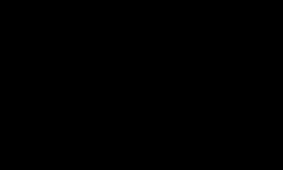
\includegraphics[width=85mm]{./imgs/im1.jpg}
\caption{\tiny{\Formular{\index{Carpaccio, Vittore}Vittore Carpaccio. {\slsc{Retorno dos embaixadores}} (1495)}}}

\end{figure}

É justamente na composição da cena onde podemos encontrar uma espécie de
ato ``subversivo'' em relação à perspectiva. Se o espaço é, como se
espera, estático e perfeito, a cena é puro movimento e, principalmente,
\emph{narrativa}. Percebemos um personagem em movimento, em direção ao
grupo que o espera sob o pavilhão, obedecendo a um protocolo
cerimonioso. Há uma história se desenrolando, uma ação que se desenvolve
no tempo, com início e fim, da esquerda para direita, como nossa leitura
textual. Há toda uma descrição rica e sofisticada do espaço, com
diversos detalhes a respeito da arquitetura, das roupas, da organização
social e política. Na tela de Carpacccio, segundo \index{Argan, Giulio Carlo}Argan (2003a, p.~367),
``o olho não se limita a receber: indaga, revista, percorre, conecta,
reporta''. A narrativa, que é também relato, percurso e movimento, se
opõe à estática impositiva e científica do ``instrumento visual''.
\index{Carpaccio, Vittore}Carpaccio percebe que a perspectiva é um instrumento de
criação espacial e acredita que é apenas isso o que deve ser: um cenário
a serviço da ação e da imaginação.

\chapter{Canaletto e Velázquez}

Poucos artistas dominaram tão bem a técnica da perspectiva quanto
\index{Vermeer, Johannes}Vermeer (1632-1675) e \index{Canaletto}Canaletto (1697-1768). Os interiores iluminados
pela janela lateral, no caso de um, e as paisagens de Veneza, no caso do
outro, criam uma ilusão espacial tão crível que às vezes pensamos estar
diante de uma fotografia. Com o Iluminismo, um novo olhar mais objetivo
e científico é imposto à realidade e a precisão da representação
pictórica da paisagem é um dos campos em que esta nova visão do mundo se
manifesta.

\index{Canaletto}Canaletto, que iniciou sua carreira como cenógrafo, dominava de tal
forma a disposição dos elementos arquitetônicos no espaço que chegava a
deslocá"-los caso a disposição real não lhe agradasse. O artista podia
aumentar o tamanho da torre, acrescentar janelas ou deslocar uma coluna
em nome da harmonia do conjunto (nesse sentido, um precursor da
manipulação digital). \index{Canaletto}Canaletto utilizava o ponto de fuga e se valia de
jogos de luz e sombra para criar uma sensação de profundidade mais
intensa do que se criada apenas com as regras rígidas da perspectiva. Em
nome do equilíbrio e da composição, fazia uso da técnica para
``corrigir'' a própria realidade mostrando que a simples aplicação das
regras da perspectiva podia resultar numa obra perfeita, mas
desinteressante. Em resumo, não existe arte sem imaginação, como sugere
\index{Argan, Giulio Carlo}Argan (2003a, p.~366): ``também a imaginação é um processo da mente
humana e os fatos que produz (as imagens) são reais e devem tornar"-se
visíveis como cada coisa real''.

A tela \emph{Campo Santi Giovanni e Paolo} (1735-1738) mostra um arranjo
arquitetônico que não se pode obter a partir de apenas um ponto de
vista. Aqui, Canaletto combina pelo menos dois para compor o quadro. Ao
mesmo tempo em que a fachada da igreja se mostra frontalmente (o que só
pode ser obtido a partir da ponte que se vê à esquerda), a lateral e o
resto da composição apontam para um ponto de fuga bastante pronunciado à
direita da composição, no nível do observador. Ali convergem tanto as
linhas arquitetônicas quanto o pavimento da rua lateral. As diagonais
produzidas pelas sombras, sobretudo aquela que prolonga a fachada
lateral da igreja, acentuam esse efeito dramático que direciona o olhar
para o infinito, para o ponto onde a rua desaparece na distância,
criando a sensação de profundidade necessária, mas sem tirar o foco dos
elementos principais. O resultado é uma composição descritiva,
estereoscópica e paraláctica, que mostra o edifício em elevação e em
perspectiva simultaneamente, mas sem abusar de distorções que pudessem
destruir a naturalidade da composição.\footnote{A elevação e a
  perspectiva são as duas formas básicas de representação realista da
  arquitetura, adotadas tanto pelo desenho quanto pela fotografia. A
  elevação é bidimensional e mostra a fachada da estrutura vista de um
  ponto de vista estritamente frontal. A vista em perspectiva mostra o
  edifício colocado diagonalmente no espaço, criando uma ilusão de
  tridimensionalidade. Essa ilusão é ressaltada com o uso da luz
  direcionada, que dá profundidade à cena e textura às superfícies. Na
  perspectiva, diferentemente da elevação, o contexto é importante e
  elementos como árvores, veículos, nuvens e, principalmente, pessoas
  são usados para situar o observador no espaço. Enquanto a elevação
  serve como uma representação diagramática que transmite as informações
  essenciais sobre a fachada e suas proporções corretas, a perspectiva
  tenta simular a verdadeira experiência de ver o edifício (ou projeto)
  em seu contexto real (ou pretendido).} A obra restaura não exatamente
a imagem ``real'' que se vê no local, mas a imagem ``ideal'', tal como
se preserva na memória, resultado da experiência de ter percorrido esse
lugar, dos sentimentos subjetivos que desperta e da combinação de
distintos pontos de vista, incluindo assim, sutilmente, uma dimensão
temporal à obra. Mas a tela de \index{Canaletto}Canaletto não pretende ser apenas o
resultado da experiência pessoal do pintor. Com suas regras, clareza e a
positividade, almeja estabelecer uma base comum de entendimento entre os
indivíduos de sua época.

\begin{figure}[!ht]

\centering
 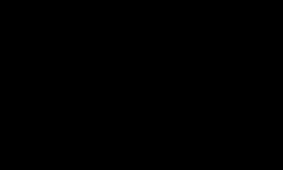
\includegraphics[width=85mm]{./imgs/im1.jpg}
\caption{\tiny{\index{Canaletto}\Formular{Canaletto. {\slsc{Campo Santi Giovanni e Paolo}} (1735-1738)}}}

\end{figure}

Esse tipo de pintura, chamada de \emph{veduta}, vai encontrar terreno
fértil na Veneza do século \versal{XVIII} como o princípio de uma nova cultura,
fundada na positividade da experiência visual (\versal{ARGAN}, 2003a, p.~366). As
próprias características da cidade flutuante, onde a natureza e a arte
se encontram, com a qualidade de sua luz refletida nas águas e nos
palácios, sua vocação marítima conectada ao Oriente, favorecem uma
cultura, como diz \index{Argan, Giulio Carlo}Argan (2003a, p.~366), ``orientada a antepor o valor
da experiência ao da ideia''. O \emph{vedutismo}, muito mais do que um
mero gênero pictórico é, antes, uma sofisticada forma de ver, produto da
relação particular entre um local (Veneza) e um tempo (o Iluminismo)
específicos.

Tanto \index{Canaletto}Canaletto quanto \index{Vermeer, Johannes}Vermeer podem ter usado a \emph{câmera obscura}
na elaboração de suas telas e há um caloroso debate acerca disso. Esse
aparelho, conhecido desde a Antiguidade, é literalmente uma câmera, ou
seja, uma caixa escura que, através de um orifício ou de uma lente,
projeta a imagem invertida na superfície oposta.\footnote{A ``invenção''
  da fotografia não é nada mais do que a fixação dessa imagem numa
  superfície fotossensível.} Alguns acreditam que seu uso na pintura
seria uma ``trapaça'', sendo o desenho obtido através da observação
direta um método mais nobre.\footnote{A rigor, mesmo uma imagem obtida
  exatamente a partir de um único ponto de vista, como numa fotografia,
  carrega algo de artificial, uma vez que a visão humana é
  estereoscópica e, como nessa pintura de \index{Canaletto}Canaletto, combina dois pontos
  de vista para criar a sensação de tridimensionalidade.} Mas hoje
sabe"-se que seu uso era bastante restrito por limitações técnicas e,
mesmo com o Renascimento e o desenvolvimento de lentes mais
sofisticadas, a câmera escura nunca chegou a substituir o uso da \label{canaletto}
perspectiva linear. É possível que \index{Canaletto}Canaletto tenha usado o aparelho como
instrumento auxiliar, mais como técnica \emph{iluminista} que ``limpa''
a imagem, que verifica e atesta o dado visual, do que como um ofício
\emph{ilusionista}, que tenta enganar o observador, como na pintura
barroca cujo objetivo era justamente confundir as ideias através da
ilusão.

\index{Canaletto}Canaletto foi um pintor bastante comercial. Seus quadros eram quase
todos destinados a clientes ingleses ávidos por imagens ``exóticas'' de
Veneza, como cartões"-postais, e é frequentemente ``acusado'' de
manipulação e de ``trapaça''. Se é verdade que não se pode creditar a
ele o mérito de ter questionado criticamente a perspectiva, também é
verdade que soube utilizar"-se dela não apenas como reprodutora fria dos
volumes, mas como meio criativo que dá vida aos lugares. Na sua obra, a
perspectiva é o que deveria ser: um instrumento a serviço do artista e
não uma imposição autoritária que submete o mundo às suas regras.
\index{Canaletto}Canaletto mostra que ``ética'' visual é um conceito duvidoso quando
aplicado ao universo criativo da arte, e que a verdade da
\emph{costruzione legittima} pode estar mais próxima da imaginação do
que da realidade.

O ponto de vista único também pode ser entendido como aquele
que permite ver uma cena como que através de um buraco de fechadura
(lembremos que, para isso, é preciso fechar um dos olhos), portanto
garantindo anonimato ao observador. Nesse sentido, podemos dizer que há
algo de \emph{voyeurístico} na visão em perspectiva. De fato, uma visita
a um museu de pinturas como o Museu do Prado, em Madri (um lugar
\emph{voyeurístico} por excelência), é uma experiência às vezes
constrangedora, uma vez que podemos observar a intimidade de diversos
personagens da história, sem sermos vistos.
Mesmo antes de \index{Canaletto}Canaletto podemos encontrar na arte exemplos de obras que
tentaram usar a perspectiva de forma criativa e, por vezes, crítica. Uma
obra emblemática é, sem dúvida, o quadro \emph{Las meninas} (1655), de
\index{Velázquez, Diego}Diego Velázquez. 

Essa composição é construída obedecendo rigorosamente as regras da
perspectiva linear, com um ponto de fuga bastante centralizado, que
``suga'' o observador para dentro do quadro numa espécie de ``queda para
frente'' característica das composições mais simétricas em formato de x.
O salão retratado inclusive se parece com o próprio interior de uma
\emph{câmera obscura}, como se o observador pudesse enxergar pelo
orifício do aparelho. As dimensões do quadro, com mais de três metros de
altura, colocam os personagens quase em escala humana. O observador está
situado exatamente nesse ponto de vista único que o sistema exige,
podendo ver uma cena privada da vida na corte. Mas aqui não há anonimato
possível, pois algo inusitado acontece: os personagens estão nos
observando, com curiosidade. Ao invés de olhar pelo buraco de fechadura,
é como se abríssemos a mesma porta, surpreendendo os personagens, que
reagem à nossa intrusão. \index{Velázquez, Diego}Velázquez inverte a relação e nos coloca no
desconfortável lugar daqueles que são observados. Mesmo o próprio
ambiente do salão onde estão os personagens, cheio de quadros, se parece
com o museu onde estamos, criando um efeito de espelhamento. Assim, obra
e visitante estão em lugares trocados, o olhar deixa de ser
unidirecional e o observador se torna personagem. É um quadro atraente e
incômodo ao mesmo tempo, como se o pintor quisesse que sentíssemos
aquilo que seus retratados sentem quando são pintados provocando, assim,
uma reflexão sobre a natureza dos próprios meios de representação e da
arte.

E não somos apenas observados, somos também pintados. O próprio
\index{Velázquez, Diego}Velázquez está também retratado no quadro e, graças ao espelho ao fundo,
podemos especular que está pintando um retrato da família real numa
grande tela cujas dimensões se assemelham às próprias dimensões de
\emph{Las Meninas} (simulações computadorizadas da cena em 3D mostram
que o espelho ao fundo reflete a superfície da tela que vemos do lado
esquerdo). E o pintor também nos olha. Aqui, igualmente podemos entendê"-la
como uma tela transparente, uma janela aberta entre dois ambientes,
entre dois mundos curiosos um pelo outro. Uma das leituras possíveis (há
muitas) é que nós (o observador) estamos, portanto, ocupando o lugar da
família real e sendo retratados por\ldots{} \index{Velázquez, Diego}Velázquez! Talvez seja esse o
maior fascínio que o quadro exerce: enquanto observamos \emph{Las
Meninas}, e somente nesse momento, seremos reis da Espanha.

Pelo retrato de um instante preciso, pela naturalidade dos personagens,
pelo jogo de olhares, pela perspectiva rigorosa, pelo comportamento da
luz, pela sofisticação ótica\emph{, Las Meninas} é um quadro
extremamente fotográfico. A cena é vista não só a partir de um ponto
preciso no espaço, mas também de um ponto preciso no tempo. É o
congelamento de um instante, uma suspensão do tempo, como numa
fotografia. Aqui sim, se faz valer o (quase sempre mal compreendido)
``instante decisivo'' associado ao fotógrafo \index{Cartier-Bresson, Henri}Henri Cartier"-Bresson. Não
simplesmente um flagrante, não um momento fugaz prestes a se desmanchar
(como qualquer momento é), mas a conjunção precisa dos elementos do
espaço vistos partir de um único ponto de vista, num único ponto do
tempo --- uma relação corporal e visual entre o observador e aquilo que
observa. É como se o observador, as figuras e o cenário fossem corpos
celestes em movimento que de repente entrassem em harmonia cósmica, como
num alinhamento astronômico.

\begin{figure}[!ht]

\centering
 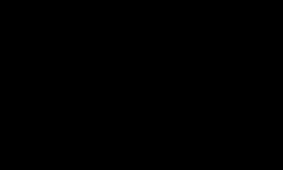
\includegraphics[width=85mm]{./imgs/im1.jpg}
\caption{\tiny{\Formular{\index{Velázquez, Diego}Diego Velázquez. {\slsc{Las Meninas}} (1656)}}}

\end{figure}

Os quadros obscuros, a abertura ao fundo, o espelho e a tela que se vê
parcialmente criam enquadramentos dentro do quadro, salientando o
caráter artificial da própria ideia de ``quadro'' na sua tentativa de
ordenar a realidade. Nosso campo de visão, lembremos, tem um formato
vagamente elíptico, horizontalizado e com bordas difusas, em nada
parecido com um quadro geométrico e ortogonal (menos ainda vertical),
formato praticamente desconhecido no mundo natural. O quadro é um corte
de navalha imaginário nessa realidade, que elege com violência o que
incluir e o que excluir de si, onde o que se vê é tão importante quanto
o que não se vê (como no mapa de Bellman). Com \emph{Las Meninas}
\index{Velázquez, Diego}Velázquez nos lembra que na própria natureza da arte está o artifício e
o artificial, ao mesmo tempo em que celebra o próprio ato de ver como
gesto primordial da pintura.

Se \index{Canaletto}Canaletto se valia da perspectiva muitas vezes com intuito comercial,
\index{Velázquez, Diego}Velázquez cria múltiplos pontos de vista numa mesma obra, sugerindo uma
visão crítica da perspectiva linear utilizando, para isso, suas próprias
regras geométricas. Mas será apenas com Turner (e suas paisagens
marítimas ``indefinidas'') e, depois, com \index{Cezanne, Paul@Cézanne, Paul}Cézanne, que se iniciará
propriamente o longo processo de desconstrução do espaço euclidiano
produzido artificialmente desde o Renascimento. A perspectiva linear
permaneceu como padrão visual até o surgimento do cubismo, no início do
século \versal{XX}, que inaugurou uma verdadeira ``revolução ótica''. Ali, o
ponto de vista único do Renascimento foi finalmente multiplicado em
diversos pontos de vista, nenhum deles superior aos outros, cada um
propondo uma leitura diferente da imagem. Os objetos se decompõem e
passam a se mostrar de todos os lados, frente e verso simultaneamente,
acrescentando uma nova dimensão temporal às três dimensões espaciais da
Renascença.

\chapter{A imagem estilhaçada}

A partir do cubismo o observador passa a recusar o espaço
exaustivamente descrito a partir de um único ponto de vista e é impelido
a movimentar"-se nesse espaço. O resultado é uma imagem multifacetada,
estilhaçada e caleidoscópica, produto de uma nova percepção do ambiente
em consonância com a ideia de velocidade e simultaneidade que passou a
caracterizar a vida moderna. Segundo \index{Argan, Giulio Carlo}Argan (1992, p.~366), não se trata
de apresentar diversos aspectos do objeto, mas várias ``verdades''
diferentes, nenhuma mais verdadeira que a outra. O cubismo é, portanto,
o primeiro passo para o abandono do ponto de vista único e estático,
abrindo caminho para novas formas de representação que precisam
considerar as complexidades e dinâmicas de um mundo em transformação,
sobretudo impulsionadas pelos avanços sociais e tecnológicos. Não são
poucas essas inovações que vão transformar nossas concepções até então
estabelecidas de espaço e tempo, como percebe \index{Virilio, Paul}Paul Virilio:

\begin{quote}
Desde o início do século \versal{XX} a profundidade de campo das perspectivas
clássicas foi renovada pela profundidade de tempo das técnicas
avançadas. O desenvolvimento da indústria cinematográfica e da
aeronáutica seguiu de perto a abertura dos grandes bulevares. Ao desfile
\index{Haussmann, Georges-Eugène}haussmanniano sucedeu"-se o desfile acelerado de imagens dos irmãos
Lumière, à esplanada dos Invalides sucedeu"-se a invalidação do plano
urbano, a tela bruscamente tornou"-se o local, a encruzilhada de todos os
meios de comunicação de massa (1993, p.~19).
\end{quote}

Não é por acaso que em \emph{Nu descendo uma escada nº 2} (1912), tela
definidora do cubismo, \index{Duchamp, Marcel}Marcel Duchamp tenha se inspirado diretamente nos
estudos do movimento de \index{Marey, Étienne-Jules}Étienne"-Jules Marey e \index{Muybridge, Eadweard}Eadweard Muybridge. Esses
experimentos utilizavam a técnica fotográfica para criar sequências de
imagens que simulavam o movimento, prenunciando o surgimento do cinema.
Em \emph{Mulher descendo a escada} (1887), de \index{Muybridge, Eadweard}Muybridge, é possível
reparar, graças ao congelamento fotográfico, numa série de movimentos do
corpo que passam despercebidos ao olhar humano. A obra de \index{Duchamp, Marcel}Duchamp parece
sobrepor todos esses movimentos numa só tela, dando conta não só dos
diversos pontos de vista, mas também da passagem do tempo.

\begin{figure}[!ht]

\centering
 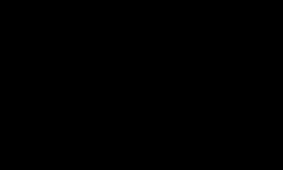
\includegraphics[width=85mm]{./imgs/im1.jpg}
\caption{\tiny{\Formular{\index{Duchamp, Marcel}Marchel Duchamp. {\slsc{Nu descendo uma escada nº~2}} (1912)}}}

\end{figure}

\begin{figure}[!ht]

\centering
 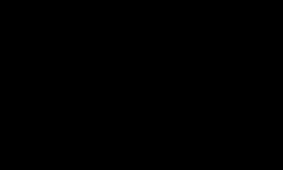
\includegraphics[width=85mm]{./imgs/im1.jpg}
\caption{\tiny{\index{Muybridge, Eadweard}\Formular{Eadweard Muybridge. {\slsc{Mulher descendo a escada}} (1887)}}}

\end{figure}


Além do cubismo, outras formas de visualizar a realidade vão surgindo ao
longo da primeira metade de século \versal{XX}. A fotografia começa a mostrar  aquilo que o olho humano não é capaz de ver, as colagens e a pintura abstrata ignoram por completo a própria ideia de profundidade, a montagem cinematográfica articula tempos e espaços de uma forma nunca antes vista.\footnote{Vale lembrarmos aqui do texto"-manifesto escrito pelo cineasta soviético \index{Vertov, Dziga}Dziga Vertov, que revolucionou a técnica cinematográfica com o filme {\slsc{Um homem com uma câmera}} (1929), utilizando múltiplas exposições, câmera lenta, cortes, telas divididas e ``travellings'', entre outras inovações: ``I am kino-eye, I am a mechanical eye. I, a machine, show you the world as onty I can see it.
Now and forever, I free myself from human immobility, I am in constant motion, I draw near, then away from objects, I crawl under, climb onto them. I move apace with the muzzie of a galloping horse, I plunge full speed into a crowd, I outstrip running soldiers, I fall on my back, I ascend with an airplane, I plunge and soar together with plunging and soaring bodies. Now I, a camera, fling myself along their resultant, maneuvering in the chaos of movement, recording movement, starting with movements composed of the most complex combinations.
Freed from the rule of sixteen-seventeen frames per second, free of the limits of time and space, I put together any given points in the universe, no matter where I've recorded them.
My path leads to the creation of a fresh perception of the world. I decipher in a new way a world unknown to you''. Ver \scalebox{.8}{MICHELSON}, Annette (ed.). {\slsc{Kino-Eye: The Writings of \index{Vertov, Dziga}Dziga Vertov}}. Berkeley: University of California Press, 1984, p.~17 (trad.~minha). Publicado originalmente em 1923 na revista de vanguarda {\slsc{\scalebox{.8}{LEF}}} ({\slsc{Frente de esquerda das artes}}), fundada por \index{Brik, Osip}Osip Brik e \index{Maiakovski, Vladimir}Vladimir Maiakovski.} No
teatro, a relação plateia"-palco, até então unidirecional, passa por uma
revolução com a ``derrubada da quarta parede'', borrando a separação
entre a ficção representada e a realidade do público.\footnote{O mundo
  como um teatro ({\slsc{Theatrum mundi}}) é uma importante metáfora do
  século \scalebox{.8}{XVII}, presente em várias obras da literatura como em {\slsc{As
    you like it}} (1623), de \index{Shakespeare, William}Shakespeare: ``All the world's a stage,/ And all the men and women merely players:/ They have their
  exits and their entrances;/ And one
  man in his time plays many parts'' (2010, p.~51).} A teoria da
relatividade e a física quântica passam a questionar não só a
arbitrariedade do ponto de vista como também a integridade dos próprios
objetos. O olho natural, ``em estado selvagem'', se liberta das leis
restritivas da arte e está agora em busca de harmonia com as leis da
natureza.

Na arquitetura, o uso do vidro promove a ideia de transparência como
metáfora da verdade e da razão. Enquanto isso, \index{Le Corbusier}Le Corbusier introduz o
conceito de \emph{promenade architecturale} (passeio arquitetural), que
valoriza o percurso e os diversos pontos de vista possíveis para a
apreciação do edifício em movimento, estabelecendo hierarquias,
ordenações e surpresas visuais. A arquitetura passa a ter (ou recupera)
uma dimensão temporal, ``narrativa'', onde o \emph{mapeamento} do
edifício e de seu terreno é mais importante que o impacto de uma fachada
espetacular vista de frente.

Nesse contexto de transformação, um papel bastante especial foi
reservado à fotografia. Instrumentos como a \emph{câmera obscura}, o
telescópio e o microscópio já haviam revelado todo um mundo de coisas
antes inacessíveis aos olhos humanos, mas o impacto visual causado pela
fixação da imagem fotográfica sobre o papel não apenas amplia o acesso
às coisas que há para ver como transforma nossa própria forma de ver.

Sem querer entrar mais profundamente no debate sobre a natureza da
imagem fotográfica, cabe perceber a relação da fotografia com a
perspectiva linear. O sistema renascentista representa uma primeira
mecanização do olhar que vai se desenvolver enormemente com a fotografia
e, posteriormente, nos diversos aparelhos que usamos hoje em dia, numa
linha evolutiva. A imagem capturada pela câmera escura, projetada na
superfície fotossensível e eventualmente impressa numa folha de papel
apresenta as mesmas características geométricas da imagem pictórica
criada a partir das regras da perspectiva. Tanto o ponto de fuga quanto
a diminuição dos objetos conforme a distância --- os principais elementos
que criam a sensação de profundidade --- são dados visuais produzidos
pelas duas técnicas, uma vez que ambas supõem a existência de um único
ponto de vista organizador da imagem.
Mas com uma diferença fundamental. Aquilo que através da perspectiva é
produzido aplicando complicadas regras geométricas --- num processo
sofisticado e lento, que exige anos de treino por parte do artista --- é
realizado pela câmera fotográfica num instante. Em outras palavras, a
câmera fotográfica é uma máquina automática de criação de \label{automatica}
perspectiva.\footnote{Se concordarmos com o argumento de \index{Argan, Giulio Carlo}Argan, de que a
  perspectiva é um processo criador da própria beleza, teríamos que
  admitir que a câmera fotográfica é uma máquina de criação automática
  de beleza --- o que talvez explique a sensação de belo que temos diante
  de uma fotografia que retrata uma situação degradante ou uma tragédia,
  como nas fotos de \index{Salgado, Sebastião}Sebastião Salgado, por exemplo. A ``beleza'' dessas
  fotos seria a beleza de qualquer foto, ou seja, a beleza da própria
  realidade reproduzida com ``perfeição''.}

\begin{figure}[!ht]

\centering
 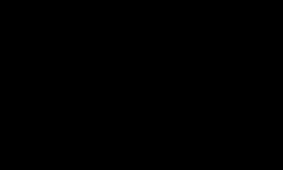
\includegraphics[width=85mm]{./imgs/im1.jpg}
\caption{\tiny{\index{Marville, Charles}\Formular{Charles Marville. {\slsc{Boulevard Saint"-Germain}} (1877)}}}

\end{figure}

Dessa forma, essa apreensão mecânica e instantânea da realidade vai ter
um impacto profundo no desenvolvimento da arte. Diante da facilidade e
da fidelidade com que a câmera fixa a imagem, a responsabilidade pela
documentação do mundo passou da pintura para a fotografia.\footnote{Não
  por acaso, muitos dos primeiros fotógrafos eram ex"-pintores. Segundo
  \index{Baudelaire, Charles}Baudelaire (2007, p.~12), a fotografia é o ``refúgio dos pintores
  fracassados, mal"-dotados ou preguiçosos''.} Já não havia razão para
que se pintassem paisagens e retratos apenas com o intuito de
``registrar'' aquele cenário ou aquela pessoa para a posteridade pois a
fotografia faria este trabalho de forma mais eficaz e mais barata.

Como consequência, tendo a fotografia libertado a pintura da responsabilidade
de descrever o mundo, permitiu seu desenvolvimento formal, que resultou
no cubismo e, posteriormente, na pintura abstrata, que acabaram por
desconstruir a perspectiva linear. Portanto, a fotografia, por um lado,
prolonga e reafirma a existência da perspectiva, ``naturalizando'' essa
forma de ver o mundo até hoje, mas, por outro, dispara o processo que
vai culminar com sua desconstrução pela própria pintura.

Demorou muito para que a fotografia, caracterizada durante décadas por
essa prorrogação da visão perspéctica, se juntasse à pintura na
contestação da perspectiva linear. O trabalho do artista holandês \index{Dibbets, Jan}Jan
Dibbets, por exemplo, é uma reflexão bastante precisa e sucinta acerca
esse tema. Numa imagem da série (justamente chamada) \emph{Perspective
correction} (1967-1969), a câmera transforma um quadrilátero irregular
desenhado na parede oblíqua num quadrado perfeito, de modo que não
sabemos mais qual dos dois é o mais ``verdadeiro''. Com isso, \index{Dibbets, Jan}Dibbets
subverte as regras da fotografia e ``engana'' a câmera, --- justamente
esse instrumento que vem nos iludindo desde a Antiguidade --- e faz com
que ela mesma mostre involuntariamente seu artifício.

\begin{figure}[!ht]
\centering
 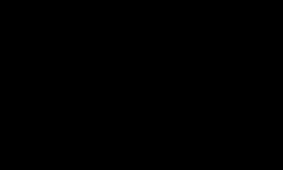
\includegraphics[width=85mm]{./imgs/im1.jpg}
\caption{\tiny{\Formular{\index{Dibbets, Jan}Jan Dibbets. {\slsc{Perspective correction}} (1968)}}} 
\end{figure}

Hoje, parece que convivemos com múltiplas formas de visualização do
espaço, sendo a perspectiva apenas uma delas. Esse processo de
desconstrução foi, aos poucos, desmontando o que \index{Virilio, Paul}Virilio chamou de
``ortodoxia ortogonal'':

\begin{quote}
A crise da noção de dimensão, portanto, surge claramente como a crise do
inteiro, a crise de um espaço \emph{substancial} (contínuo e homogêneo)
herdeiro da geometria arcaica, em benefício da relatividade de um espaço
\emph{acidental} (descontínuo e heterogêneo) em que as partes, as
frações (pontos e fragmentos diversos) tornam"-se novamente essenciais
(\versal{VIRILIO}, 1993, p.~27).
\end{quote}

Com isso, o espaço euclidiano, até então ``absoluto'', entra em crise.
Nosso tradicional sentido de orientação foi profundamente abalado.
Referências estáveis como a linha do horizonte e os pontos de fuga
desaparecem e já não é mais possível, como aponta \index{Latour, Bruno}Latour (\versal{NOVEMBER};
\versal{CAMACHO"-HÜBNER}; \versal{LATOUR}, 2013, p.~10), aceitar um mundo feito de
``objetos galileanos'' atravessando um ``espaço euclidiano'', que a
perspectiva linear e, posteriormente, a geometria descritiva haviam
propagado como perfeito.

\chapter{As coisas como elas são}

Imagine ser por um instante um laboratorista que precisa fazer uma cópia
de uma fotografia muito famosa. Imagine ter em mãos, por exemplo, o
negativo de \emph{Atrás da Estação St. Lazare} (1932), de \index{Cartier-Bresson, Henri}Henri Cartier"-Bresson ou \emph{Guerrilheiro heroico} (o célebre retrato de \index{Guevara, Che}Che
Guevara, de 1960), de \index{Korda, Alberto}Alberto Korda, ou uma das grandes placas de vidro
que \index{Ferrez, Marc}Marc Ferrez utilizou para retratar o Rio de Janeiro. Imagine ver
esses objetos translúcidos através de uma lupa, pousados sobre uma mesa
de luz. Basta tocá"-los para perceber que se trata de algo extremamente
delicado e precioso.

O negativo é esse belíssimo objeto que, junto com o fotógrafo e a
câmera, ``esteve lá'', diante da cena. Uma vez exposto à luz, teve sua
estrutura físico"-química irreversivelmente transformada pela incidência
direta dos raios luminosos refletidos pelo objeto fotografado. Por isso,
a imagem captada com películas fotossensíveis ainda guarda uma relação
\emph{indicial} com aquilo que representa.

É curioso pensar --- a partir do célebre texto de \index{Benjamin, Walter}Walter Benjamin,
\emph{A obra de arte na era de sua reprodutibilidade técnica} (1935-1936)
--- que a fotografia é sem dúvida o caso exemplar da obra de arte
tecnicamente reprodutível mas, ao mesmo tempo, o filme fotográfico
revelado (seja ele negativo ou diapositivo), é um objeto único e
irreprodutível e, portanto, possuidor de ``aura'', essa qualidade
simbólica que confere autenticidade e ``valor de culto'' a esses
objetos.\footnote{Ver página \pageref{benjamin}.} Segundo \index{Benjamin, Walter}Benjamin
(1985, p. 173), em oposição ao ``valor de exposição'', o mais importante
em relação os objetos com valor de culto é que eles \emph{existam}, e
não necessariamente que sejam vistos. Assim é o negativo fotográfico,
guardado em algum lugar seguro, manipulado raramente.

E esse objeto não é exatamente como a matriz em madeira de uma gravura
ou a fôrma de uma escultura. A película, constituída pela base plástica
e pela emulsão química, mesmo após o processo de fixação, ainda reage
lentamente à luz e envelhece. Há uma perda gradativa e irreversível da
imagem que, aos poucos vai ``esmaecendo'' e, um dia, desaparecerá para
sempre. Ela é o suporte da própria imagem, como se a carregasse consigo.
Se não pode ser chamado exatamente de fotografia ``original'', uma vez
que ainda não se transformou plenamente numa forma de exibição, todas as
informações visuais que depois veremos na fotografia final já estão
ali.\footnote{O fotógrafo norte"-americano \index{Adams, Ansel}Ansel Adams comparava a
  fotografia com a música clássica --- o negativo sendo a partitura e a
  cópia fotográfica, a interpretação. Assim, cada laboratorista poderia
  {\slsc{interpretar}} o negativo à sua maneira.}

Pensemos, por exemplo, em \emph{The blue marble} (a bola de gude azul), \label{marble}
a mais famosa fotografia do planeta Terra, realizada pelos astronautas a
bordo da missão lunar \index{Apollo 17}Apollo 17, em 1972. A fotografia é creditada à
tripulação da missão como um todo, e foi feita em película diapositiva
com uma câmera \emph{Hasselblad} especialmente modificada. Aquela foi a
última vez que um ser humano se afastou da Terra a uma distância
suficiente para poder enxergá"-la por inteiro. Não há dúvida de que o
diapositivo da \emph{Blue marble}, seguramente guardado pela \versal{NASA} como
um pequeno tesouro de valor incalculável, carrega consigo a ``aura'' de
ser a materialização de uma das mais raras e belas imagens já vistas por
um ser humano.

Posteriormente, outras fotos da Terra foram realizadas por sondas,
veículos não"-tripulados ou a partir da fusão de várias imagens digitais.
Inclusive há uma nova série dessas fotografias (também chamadas
\emph{Blue marble}), que apresenta a Terra de uma maneira espetacular,
mas impossível de ser vista com os próprios olhos. São dados
transmitidas por satélite e manipulados posteriormente, num processo que
escolhe o melhor fragmento de cada imagem captada, elimina nuvens
indesejadas, realça cores e aumenta o contraste (além de colocar os
Estados Unidos no centro da fotografia). São muito mais nítidas e
detalhadas do que a fotografia trazida pela \index{Apollo 17}Apollo 17, mas nenhuma delas
é este objeto único que, de fato, ``esteve lá''.

Podemos entender o filme fotográfico como uma espécie de \emph{decalque}
da cena, como se a abertura do obturador da câmera permitisse que os
elementos visuais imprimissem a si mesmos diretamente na película, sem a
intervenção do fotógrafo. Na captura digital, diferentemente, a luz é
convertida e codificada numa longa sequência numérica que depois precisa
ser processada para se tornar imagem novamente, na tela do computador.
Com isso, a relação indicial que o negativo representa deixa de existir.

Quero com isso salientar esse aspecto que foge ao texto de \index{Benjamin, Walter}Benjamin:
apesar da natureza essencialmente reprodutível da fotografia, ela ainda
carregava algum aspecto ``aurático'', pela existência da matriz única em
película, geralmente um negativo.\footnote{Os concursos de fotografia
  muitas vezes exigiam dos premiados a apresentacão do negativo como
  forma de provar tanto a autoria quanto a autenticidade da imagem.
  Hoje, mesmo que haja um arquivo ``original'' (chamado {\slsc{\scalebox{.8}{RAW}}}, ou
  ``cru'') que contém todas as informações captadas na cena, as fotos
  digitais passam obrigatoriamente por um processo de ``pós"-produção''
  no {\slsc{software}}. Com isso, os concursos têm dificuldade para
  definir os limites da manipulação e, eventualmente, fraudes acontecem.}
Agora, o equivalente digital da película, ou seja, o ``arquivo''
informático que registra a sequência numérica codificada, pode ser
replicado, transmitido e armazenado, conservando sua integridade; pode
ser usado indefinidamente para a impressão de novas cópias fotográficas
sem qualquer perda de qualidade e (a não ser por um grande descuido ou
por um catastrófico ``apagamento'' digital) existirá para sempre.\footnote{Pessoalmente,
  sempre que faço uma simulação mental de um incêndio, perguntando"-me o
  que salvaria em primeiro lugar, respondo: o arquivo de negativos.}
Mais ainda, conforme são introduzidos no mercado novos \emph{softwares}
e impressoras de tecnologia superior, as impressões no futuro serão
melhores que as de hoje. Diferentemente do negativo, aqui há apenas
``valor de exposição''. Assim, com a codificação total da imagem digital,
o prognóstico de \index{Benjamin, Walter}Benjamin agora se realiza plenamente. As noções de
autenticidade e originalidade que tinham sofrido um abalo com o advento
das ``imagens técnicas'', agora acusam o golpe definitivo com a
possibilidade de ``reprodutibilidade total''.\footnote{É sintomático que,
  ao mesmo tempo em que a fotografia chega na fase de
  ``reprodutibilidade total'', os fotógrafos"-artistas passem a numerar
  suas fotos em séries limitadas --- basicamente uma estratégia de
  mercado, na tentativa artificial de fazer da cópia fotográfica um
  objeto com ``valor de culto''.}

Podemos pensar também que o negativo, com sua natureza misteriosa e
delicada, que esconde uma imagem a ser \emph{revelada}, se aproxima de
uma determinada ideia de erótico. Lembremos do laboratório fotográfico,
esse ambiente escuro e silencioso, iluminado minimamente por luzes
vermelhas e misteriosas, repleto de odores estranhos. Ali, o papel
fotográfico passa por várias etapas, a partir da abertura da caixa onde
repousa num envelope preto selado. Depois disso, é colocado na base do
ampliador, esse aparelho que projeta a imagem do negativo na superfície
do papel fotossensível. Exposto brevemente à luz que trespassa o
negativo colocado delicadamente no aparelho, o material fotossensível
que recobre o papel (a emulsão) sofre uma alteração em sua estrutura
química, acusando as informações luminosas dadas pelo negativo. No
entanto, ainda não há imagem para ser vista, pois ela está --- como se
diz --- em ``estado latente'', aguardando os banhos químicos que traduzirão
essas informações luminosas em preto, branco e gradações de cinza, em
relação oposta às tonalidades do negativo. Qualquer um que já tenha
ampliado uma fotografia num laboratório fotográfico há de lembrar"-se do
momento em que a imagem sobre o papel, imerso na banheira do revelador,
surge lentamente, como mágica.

Isso tudo remete a um universo sensível com o qual a fotografia digital
não pode sonhar. O processamento digital se dá em ambiente anódino,
limpo, controlado. Não há cheiro, não há tato, não há movimento
corporal. Tudo é perfeitamente visível e codificado. A imagem acontece
na tela, diante do sujeito sentado no computador, em simbiose corporal
com a máquina, como se fosse parte dela. No universo digital não há
lugar para nuances ou ``zonas escuras''. Seu ideal é o da clareza
matemática, da redução da imagem a um código transmissível e
veloz.\footnote{É interessante notar os termos em francês para fotografia
  analógica e fotografia digital: {\slsc{photographie argentique}}
  (fotografia argêntica, referindo"-se à prata utilizada como principal
  material fotossensível na emulsão das películas) e {\slsc{photographie
    numérique}} (fotografia numérica).} O digital é, portanto, obsceno e
pornográfico, em sua busca da ``hipervisibilidade'', daquilo que é
``mais visível do que o visível'', para usarmos os termos de \index{Baudrillard, Jean}Baudrillard (1996, p.~49).

A tecnologia computacional da imagem chegou a tal ponto de sofisticação
que, com alguma habilidade, é possível manipular quase que infinitamente
a distribuição dos \emph{pixels} e, consequentemente, dos objetos
visuais. O antigo processo de montagem ou colagem, que cortava e colava
as fotografias, passa agora a ser feito com precisão microscópica. A
fotografia digitalizada passa a ser um monstruoso quebra"-cabeça
eletrônico composto por milhões de pecinhas, sendo possível interferir
isoladamente em cada uma delas.\footnote{Uma câmera de 30
  {\slsc{megapixel}} (relativamente comum nos dias de hoje) produz uma
  imagem com cerca de 30 milhões {\slsc{pixels}} (1 {\slsc{megapixel}} = 1
  milhão de {\slsc{pixels}}). Cada um desses {\slsc{pixels}} tem à sua
  disposição 16.777.216 combinações diferentes de cor, tonalidade,
  saturação e brilho, utilizando"-se o sistema de cores \scalebox{.8}{RGB} ({\slsc{red,
    green, blue}}), padrão da maioria dos {\slsc{softwares}} de processamento
  de imagem.} Essa espécie de ``pictorialismo digital'' resulta numa
imagem fotográfica cujos acréscimos e supressões são imperceptíveis a
olho nu --- um procedimento que coloca em suspeição o próprio caráter da
representação da fotografia e instaura permanentemente o problema da
ética sobre o fazer fotográfico. Hoje, conscientes dessas infintas
possibilidades de transformação da imagem, aprendemos a
\emph{desconfiar} das fotografias.

Se, no fotojornalismo, essa facilidade de manipulação representa um
problema ético real, nas mãos de um artista pode servir como ferramenta
criativa. O fotógrafo alemão \index{Gursky, Andreas}Andreas Gursky utiliza sofisticados
\emph{softwares} de edição de imagem para criar suas obras, manipulando
pesadamente as fotografias, seja multiplicando os pontos de fuga e
subvertendo as regras da perspectiva linear através de ``colagens'',
quanto simplesmente acrescentando e eliminando elementos.\footnote{Ver
  página \pageref{canaletto}.} O trabalho fotográfico de
campo é apenas a primeira etapa do processo, apenas a captura das
imagens na rua, para depois ser finalizada numa segunda etapa de
``pós"-produção'' no computador.

\emph{Paris, Montparnasse} (1993), por exemplo, retrata o conjunto
habitacional modernista projetado por \index{Dubuisson, Jean}Jean Dubuisson na capital
francesa. É uma elevação arquitetônica resultada de duas fotografias
realizadas separadamente, mostrando o edifício de uma maneira que não se
pode ver \emph{in loco}, pela falta de recuo necessário para captar toda
a fachada numa única tomada. Com esse gesto de fusão (que depois será
aprimorado em outros trabalhos), \index{Gursky, Andreas}Gursky desobedece (como fazem outros
tantos artistas) as regras da perspectiva linear, eliminando aquele
ponto único no qual o sujeito se coloca para ver o mundo como se olhasse
através do buraco de uma fechadura, tão característico do Renascimento e
da fotografia em geral.\footnote{Ver páginas \pageref{perspectiva} e \pageref{automatica}.}

\index{Gursky, Andreas}Gursky subverte essa vocação da fotografia e constrói um edifício de
pura frontalidade, onde todas as janelas são vistas de frente, onde
todos os pontos são pontos de fuga. O resultado é uma obra por um lado
``fria'', em acordo com a tendência ``inexpressiva'' da linhagem de
fotógrafos alemães contemporâneos mas, por outro, aberta às
complexidades que de fato experimentamos na tentativa de interpretar a
realidade multifacetada em que vivemos.

Esse efeito é enfatizado ao experimentar a obra numa galeria ou museu.
Com suas grandes dimensões, ela convida o observador a se deslocar
horizontalmente, percorrendo com os olhos cada uma das janelas do bloco
residencial. Se o casal \index{Becher, Bernd e Hilla}Bernd e Hilla Becher, mestres de \index{Gursky, Andreas}Gursky na
chamada ``escola de fotografia de Düsseldorf'', criaram suas conhecidas
``tipologias'', fotografando diversas variantes de um mesmo tipo de
edificação, e depois reunindo"-as em \emph{grids} expositivos, \index{Gursky, Andreas}Gursky
parece fazer o mesmo, mas numa única fotografia. Assim como no trabalho
do casal alemão, esta obra de \index{Gursky, Andreas}Gursky convida ao conhecimento por método
de comparação.\footnote{Ver página \pageref{grid}.} Cada janela pode ser
cotejada com as outras, todas iguais e diferentes ao mesmo tempo,
representando as diversas pessoas que vivem ali. Se as diferenças
remetem à individualidade de cada um dos moradores, a semelhança
ressalta a padronização da vida contemporânea nas grandes cidades.

\index{Gursky, Andreas}Andreas Gursky, \index{Struth, Thomas}Thomas Struth e \index{Ruff, Thomas}Thomas Ruff (chamados de ``struffsky''
pelo jornal novaiorquino \emph{Village Voice}) estão entre os fotógrafos
que levaram definitivamente a fotografia para o campo da arte
contemporânea. Utilizando"-se de procedimentos como a fusão digital, a
apropriação de imagens da ciência, o uso dos grandes formatos e de
sofisticadas ferramentas da tecnologia digital, esses fotógrafos
expandiram o horizonte da linguagem fotográfica, e colocaram a ``técnica
fria'' a serviço do distanciamento emocional, da suposta objetividade e
da aparente neutralidade. Aqui, segundo a crítica \index{Cotton, Charllotte}Charllotte Cotton (2010, p. 81), ``a ênfase recai na fotografia como um modo de ir além
das limitações da perspectiva individual, um modo de mapear a extensão
de forças, invisíveis desde a perspectiva do indivíduo isolado, que
regem o mundo natural e o mundo criado pelo homem''.

\index{Gursky, Andreas}Gursky, assim como seus colegas, acredita ser capaz de realizar uma
representação ``neutra'' da realidade, desprovida de afeto e de opinião,
como se mostrasse o mundo em toda sua verdade, objetivamente, sem
intervenção da subjetividade humana: ``eu mostro nosso mundo
contemporâneo do jeito que ele é'', diz, sem muita modéstia (\versal{NAYERI},
2018, trad. minha). A opinião pessoal é tudo aquilo que os fotógrafos
dessa vertente procuram evitar a todo custo. É como se os objetos,
lugares e situações pudessem falar por conta própria, cabendo ao artista
apenas ``mostrar''. Se considerarmos que há basicamente dois tipos de
artistas: aqueles que pretendem \emph{representar} a realidade e aqueles
que pretendem \emph{transformar} a realidade, esses fotógrafos
claramente se situam no primeiro grupo, mesmo que, para isso, tenham que
lançar mão de imagens que não são verificáveis a olho nu.

Talvez possamos entender essa postura no contexto da Alemanha
pós"-guerra, um país derrotado dramaticamente e agora traumatizado e
envergonhado por seus próprios feitos. Nesse contexto, a
``neutralidade'' pretendida pode ser tanto o resultado de uma busca
legítima da verdade depois da vivência de tanta barbárie, como também o
efeito de uma anestesia geral necessária como forma de esquecimento
dessa mesma barbárie.

Uma das primeiras descobertas de quem começa a fotografar seriamente é
que a câmera, pelo menos tecnicamente, é capaz de enxergar mais do que o
olho humano. Muitos detalhes de uma cena passam despercebidos pelo
fotógrafo no momento da captura e são percebidos apenas após a ampliação
fotográfica. E quanto maior é o tamanho do negativo ou a capacidade de
``resolução'' digital, mais detalhes são registrados.\footnote{No filme
  {\slsc{Blow"-up}} (1967), de \index{Antonioni, Michelangelo}Michelangelo Antonioni, o protagonista é um
  fotógrafo de moda que, ao ampliar seguidamente no laboratório uma
  fotografia que fez por acaso, percebe ter involuntariamente capturado
  a cena de um crime. O termo {\slsc{blow"-up}} é usado em fotografia
  justamente pare referir"-se a ampliações excessivas, que ``explodem''
  os detalhes e revelam a própria estrutura (grãos ou {\slsc{pixels}}) da
  fotografia. Em {\slsc{Blade Runner}} (1982), de \index{Scott, Ridley}Ridley Scott, há uma
  cena semelhante, talvez em homenagem ao filme de Antonioni. O detetive
  Deckard utiliza uma máquina sofisticada de ampliação para detectar um
  detalhe escondido numa fotografia. A ``máquina Esper'' do filme,
  semelhante a um computador, pode ser entendida como o equivalente
  pós"-moderno e digital do laboratório químico de {\slsc{Blow"-up}} e
  prefigura, de certo modo, as ferramentas cartográficas digitais como o
  {\slsc{Google Earth}}.} Portanto, toda fotografia de grande formato
(falo tanto da captura quanto da exibição) mostra mais do que somos
capazes de ver naturalmente --- um efeito que se torna ainda mais
evidente quando a fotografia apresenta alta qualidade de impressão e é
mostrada no ambiente controlado de uma galeria. Ali, podemos tomar todo
o tempo necessário e, confortavelmente, examinar com os olhos a cena
estática, congelada pela câmera, sem o risco de transformação temporal a
que o mundo real está submetido. Este é o encanto de uma fotografia de
\index{Shore, Stephen}Stephen Shore, por exemplo, com suas esquinas banais onde primeiramente
nada é extraordinário, mas, com o tempo e o exame minucioso do olhar, os
detalhes vão se revelando lentamente.

\index{Gursky, Andreas}Gursky, com a manipulação digital, leva essa capacidade intrínseca da
fotografia em grande formato a outro patamar. A alta definição das
imagens, a saturação cromática, a monumentalidade física das obras, as
tecnologias de impressão e montagem e, é claro, a excelência técnica do
fotógrafo, acabam criando algo que às vezes parece ``mais real do que o
real''. Trata"-se de outra forma de falsificação da realidade, não mais a
deficiência de uma ``meia verdade'', mas o excesso de ``uma verdade e
meia''. Este ``hiper"-realismo'' foi definido por \index{Baudrillard, Jean}Baudrillard como uma
simulação de um real que nunca existiu, e que acaba substituindo e
anulando a própria realidade com seu poder de sedução.\footnote{Hiper"-realismo
  é também um movimento artístico que tem origem no anos 1960,
  tributário da Pop Art e do Fotorrealismo. Enquanto esse último
  criava grandes pinturas a partir de fotografias reproduzidas
  minuciosamente na tela, o Hiper"-realismo se manifesta sobretudo na
  escultura, criando figuras tão verossímeis que parecem vivas (como no
  trabalho do australiano \index{Mueck, Ron}Ron Mueck, por exemplo). Apesar da
  impressionante sofisticação técnica, parece"-me mais um exercício
  formal de forte apelo midiático do que uma proposta de representação
  crítica da realidade.} É um fenômeno definidor da sociedade de
consumo pós"-moderna e um modo de ver que se alinha às telas de alta
definição, às plataformas cartográficas digitais, ao universo da
publicidade e ao próprio acesso à informação em época de comunicações em
rede.\footnote{Ver página \pageref{hiperreal}.} Nesse sentido, \index{Gursky, Andreas}Gursky
provavelmente preferiria a \emph{Blue marble} de 2012, digitalizada,
manipulada e supernítida, que mostra o globo terrestre idealizado, sem
as imperfeições e o acaso da fotografia de 1972.

Mas todo esse hiper"-realismo não significa necessariamente acesso a um
mundo de verdades. De fato, talvez esteja mais próximo a um novo tipo de
cegueira. Não se trata mais de uma fotografia \emph{subexposta} que
esconde os elementos na escuridão, mas de uma fotografia
\emph{superexposta}, que cega por excesso de claridade. Pois há, como
nos revela o crítico \index{Wisnik, Guilherme}Guilherme Wisnik (2018, p. 87), uma estranha
relação entre nitidez e opacidade --- duas qualidades que, embora
aparentemente antagônicas, podem servir a propósitos trocados. Assim
como o mistério e a dúvida podem ser iluminadores da verdade na medida
em que representam as imperfeições de nosso mundo imperfeito, muitas
vezes o excesso de nitidez, por seu poder inebriante e sedutor, tem como
efeito a ocultação dessa mesma verdade. Um mundo destituído de
ambiguidades, sem texturas nem desfoques, que se mostra como
``perfeito'', impede a própria ação do sujeito que tenta transformá"-lo,
restando a ele apenas uma ``leitura passiva dos seus códigos de
funcionamento'' (\versal{WISNIK}, 2012, p. 199). No fundo, este é o mesmo
problema que existe na confusão entre informação e conhecimento num
mundo onde a informação, através da internet, parece estar ``ao alcance
dos dedos'' --- uma das grandes ilusões de nosso tempo.\footnote{Ver
  página \pageref{ubiquidade}.}

O interesse na obra de \index{Gursky, Andreas}Gursky repousa em sua hábil elaboração artística
do hiper"-realismo, como se dissesse que o olhar nu e cru não basta, que a
realidade complexa em que vivemos não se dá a ver tão facilmente,
escondida para além de nossa capacidade de apreensão visual ocular. A
realidade, na proposta de \index{Gursky, Andreas}Gursky, estaria mais próxima daquilo que não
vemos do que daquilo que vemos. E, se nem o olho nem a câmera
fotográfica são capazes de enxergá"-la, será preciso criá"-la. Assim,
paradoxalmente, o artifício é usado para restaurar a verdade, para nos
aproximar de uma realidade impalpável e invisível. A máxima que diz ``é
preciso ver para crer'', que atribui aos olhos a legitimidade última da
verdade, aqui é invertida, tornando"-se ``é preciso crer para ver'' pois,
aceitando as imagens de \index{Gursky, Andreas}Gursky, o mundo complexo e globalizado em que vivemos se tornaria um pouco mais claro.

Pela pretensão, pelas dimensões das obras e pela tradição acadêmica
alemã podemos abordar o trabalho de \index{Gursky, Andreas}Gursky pela via da categoria
estética do sublime. De \index{Aristóteles}Aristóteles a \index{Lyotard, Jean-François}Lyotard, passando por \index{Kant, Immanuel}Kant e
\index{Hegel, Georg Wilhelm Friedrich}Hegel, o sublime refere"-se a uma beleza grandiosa, assombrosa e
desmesurada, que ultrapassa a capacidade humana de apreensão direta e
não pode ser totalmente compreendida. É uma beleza que flerta com o
trágico e com o divino, que impõe uma força de cima para baixo,
ameaçando a fragilidade humana.\footnote{Na última estrofe do Canto \scalebox{.8}{I} do
  poema épico {\slsc{Os Lusíadas}} (1572), o poeta português \index{Camões, Luís de}Luís de Camões
  oferece uma imagem exemplar do sublime na literatura: ``No mar tanta
  tormenta e tanto dano,/ Tantas vezes a morte apercebida!/ Na terra
  tanta guerra, tanto engano,/ Tanta necessidade avorrecida!/ Onde pode
  acolher"-se um fraco humano,/ Onde terá segura a curta vida,/ Que não
  se arme e se indigne o Céu sereno/ Contra um bicho da terra tão
  pequeno?''. Ver \scalebox{.8}{CAMÕES}, Luís de. {\slsc{Os Lusíadas}}. 4. ed. Lisboa: Instituto
  Camões, 2000, p. 27.} Dessa forma, o sublime pode tanto
esmagar o sujeito, impedindo qualquer tentativa de relação entre o homem
e essa força assombrosa, quanto incitar enormemente a imaginação, levada
ao limite na tentativa de compreender esses fenômenos que escapam à
apreensão humana. Pode ser, portanto, um proposta estética válida na
tentativa de ``representar o irrepresentável'' pois implica, por
natureza, uma inadequação, um ``fracasso representacional'' que pode ser
bastante útil para a análise da realidade contemporânea, caracterizada
pelo descompasso relacional resultante do abismo entre a experiência
humana imediata e as grandes instâncias que de fato regem nossas vidas,
conforme percebidos por diversos pensadores como \index{Jameson, Fredric}Fredric Jameson, \index{Virilio, Paul}Paul Virilio e \index{Bauman, Zygmunt}Zygmunt Bauman.

A obra de \index{Gursky, Andreas}Andreas Gursky flerta com esse sublime tanto nos temas
retratados quanto na própria forma de apresentação das imagens
fotográficas. Ele retratou grandes aglomerações humanas, paisagens
grandiosas, obras de infraestrutura, grandes edifícios e uma série de
espaços ligados ao mundo financeiro, ao entretenimento, aos esportes,
aos serviços e ao comércio de um mundo interconectado. As fotografias em
grandes dimensões (graças aos avanços das técnicas de impressão digital)
e a exibição das obras isoladas nas grandes paredes dos museus e
galerias impressionam pela monumentalidade e pela própria presença
física das molduras. Nesses ambientes, acabam concorrendo diretamente
com as pinturas de grande formato, remetendo às grandes paisagens ou
batalhas na tradição da pintura europeia. É evidente uma influência do
romantismo alemão, com seus personagens pequenos e frágeis diante da
imensidão das paisagens naturais, como nas pinturas de \index{Wolf, Caspar}Caspar Wolf
(1735-1783) e de \index{Friedrich, Caspar David}Caspar David Friedrich (1774-1840).

O exagero e a desmedida próprios do sublime são usados não apenas para
mostrar a fragilidade do homem diante da força da natureza ou das
instâncias de poder que regem nossas vidas, mas também podem servir como
ferramenta crítica que, através da inverosimilhança e do absurdo acabam
por revelar a artificialidade de um mundo regido pelo consumo e pela
publicidade que, no entanto, exerce grande fascínio. Dessa forma, a obra
de \index{Gursky, Andreas}Gursky estaria representando aquilo que o filósofo brasileiro
\index{Safatle, Vladimir}Vladimir Safatle (2007, p. 53) chamou de ``sublime capitalista'', uma
imagem do grande universo do capital e de nossa sociedade competitiva,
consumista e conectada deste início de século \versal{XXI} em seu ``funcionamento
perfeito'', com todo este aparato ao mesmo tempo sedutor e opressor.

A lógica do capitalismo e da tecnociência é a busca de ``mais e mais'', de
um crescimento sem fim orientado para o acúmulo de riqueza que, por sua
vez, aprimora o conhecimento técnico para gerar ainda mais riqueza. Essa
lógica, insustentável e suicida como uma bomba"-relógio, coloca em marcha
uma sequência infinita de transformações e operações que (além de
exaurir os recursos naturais do planeta) leva a humanidade a uma
permanente frustração. Para o filósofo francês \index{Lyotard, Jean"-François}Jean"-François Lyotard,
lido por \index{Fabbrini, Ricardo}Ricardo Fabbrini (2017, p.~58), essa desmedida é o ``fato
essencial da pós"-modernidade'', que encontraria uma forma de
representação através do excesso de beleza, ligada ao sublime. Mas, se
no projeto moderno o sublime era visto como a face estética de um
projeto utópico de redenção, através da racionalidade e do triunfo da
civilização e da técnica, agora ele mostra seu lado negativo, opressor.

Nesse sentido não seriam as imagens de \index{Gursky, Andreas}Andreas Gursky, com todo seu
hiper"-realismo digital, uma tentativa de representar o irrepresentável
mundo contemporâneo submetido ao excessos do capitalismo financeiro ---
um mundo saturado de imagens, onde mídia e ambiente se fundem? Ao eleger
como tema justamente o ``espaço mundial do capitalismo multinacional''
--- chamado de ``objeto fundamental da pós"-modernidade'' por \index{Jameson, Fredric}Fredric
Jameson (2000, p. 79) ---, não seria seu trabalho uma legítima
estratégia artística de representação dessa realidade, uma tentativa de
mapear cognitivamente as forças do capital?

É incômodo pensar que esta resposta seja dada por um fotógrafo
eminentemente comercial e avesso às interpretações políticas de sua
obra.\footnote{\index{Gursky, Andreas}Gursky ganhou notoriedade depois que a obra {\slsc{99 Cent
  \scalebox{.8}{II} Diptychon}} (2001) alcançou o preço de 3.34 milhões de dólares em
  2007, tornando"-se, na época, a mais cara fotografia já vendida.} De
fato, há um problema. Diferentemente do sublime lírico que desorienta o
ser humano e carrega grande carga de violência (logo, potencialmente
perigosa e disruptiva), a estética de \index{Gursky, Andreas}Gursky é domesticada por um
``sublime formalizado'' com sua alta resolução, sua estética
publicitária e pela manipulação digital que ``limpa'' as imperfeições
indesejadas. Ao invés de um ambiente aterrador, violento e misterioso de
uma tormenta em alto mar, temos o ambiente hiperespacial de um hotel
genérico (\emph{Atlanta}, 1996), uma loja asséptica da grife Prada
(\emph{Prada I}, 1996) ou um show da Madonna (\emph{Madonna I}, 2001). O
perigo é que tal visão, com toda sua sofisticação visual, estética
publicitária e encantamento, pode fetichizar e naturalizar esse mundo
injusto e cruel que procura representar. Basta imaginarmos essas imensas
fotografias nas grandes galerias de Londres, Nova York e Frankfurt,
convertidas em fundo cenográfico de um espetáculo ostentatório. Ali, são
vendidas por alguns milhões de dólares para bilionários russos e
príncipes sauditas ao som do tilintar das melhores taças de champanhe.

\chapter{O ``olho que tudo vê''}

A perspectiva agora precisa lidar não apenas com novos pontos de vista,
mas com novas concepções de espaço. Para esses novos espaços, novas
visualidades e múltiplos pontos de vista serão necessários. E muitas
dessas imagens serão agora produzidas não apenas de modo ocular, mas
também através de mecanismos tecnológicos de captação de imagem. Uma
série de novos aparelhos como scanners e radiotelescópios associados a
softwares de modelagem 3D e de ``renderizações'' passam a produzir e
transmitir imagens não"-oculares, com qualidade e velocidade jamais
imaginadas.\footnote{Segundo alguns estudiosos estaríamos vivendo uma
  era da fotografia ``{\slsc{cameraless}}'' (sem câmera) ou
  ``pós"-fotografia''.} Para \index{Virilio, Paul}Virilio (1993, p.~23), passamos de uma visão
perspectiva para uma visão ``prospectiva'', que ``transpassa as
aparências das maiores distâncias, dos mais vastos espaços''. Com os
novos mecanismos visuais, não há visão central e visão periférica, como
no olhar humano, que distingue a todo momento o que é importante do que
é secundário.

E se há um tipo de imagem que vem se tornando cada vez mais comum são as
imagens aéreas. Essa visão bastante particular da superfície da Terra
foi uma das primeiras demonstrações daquilo que a fotografia --- e apenas
a fotografia --- podia mostrar; e marcaram um território visual que a
pintura não podia disputar. Dos primeiros experimentos realizados de
balão por \index{Nadar, Félix}Félix Nadar, no século \versal{XIX}, até as imagens aéreas de supostos
mísseis soviéticos em Cuba (que quase provocaram uma guerra nuclear),
essas imagens do alto tiveram os mais diversos usos e nos ajudaram a
planejar cidades, programar viagens e coordenar ataques, entre outros.
Mas agora escrutinam de forma inédita a superfície da Terra e passaram a
compor um novo paradigma visual com o qual estamos nos acostumando.
Fotografias feitas por satélites estabelecem um novo padrão cartográfico
e nos auxiliam nos deslocamentos mais banais, drones teleguiados
permitem uma vista de pássaro a custo acessível, câmeras de vigilância
são posicionadas no alto dos postes, sondas exploram outros planetas,
satélites particulares vendem seus serviços \emph{online}. Ao mesmo
tempo em que esse tipo de ``visualização'' se torna cada vez mais
presente, a vista em perspectiva vai se tornando apenas mais uma entre
tantas. Já não se trata de uma visão centrada no ponto de fuga, mas da
``fuga de todos os pontos'', segundo \index{Virilio, Paul}Virilio (1993, p.~67).

\begin{figure}[!ht]

\centering
 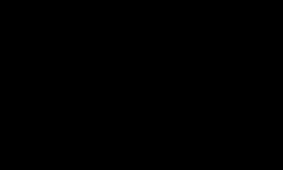
\includegraphics[width=85mm]{./imgs/im1.jpg}
\caption{\tiny{\Formular{Modelagem digital da cidade de Paris vista no {\slsc{Apple Maps}} (2018)}}}

\end{figure}

Da mesma forma que a perspectiva linear considerava a linha do horizonte
como referência estável frontal, a visão de cima para baixo, em
\emph{plongée,} transforma a própria superfície da Terra (e de outros
planetas e satélites naturais) numa espécie de ``tela'' de fundo,
bidimensional, um suporte onde as imagens se formam (lembremo"-nos das
linhas de Nazca). O olhar que antes era conduzido ao infinito em busca
do ponto de fuga, agora esbarra numa barreira intransponível. E não é
essa, justamente, a condição do mapa? No \emph{Google Maps} ou no
\emph{Apple Maps}, a fotografia da superfície da Terra captada por
satélite se funde com o próprio mapa, mostrando um mundo cada vez mais
em detalhe, a caminho de criar uma representação virtual do planeta em
escala 1:1.\footnote{Ver página \scalebox{.8}{XXXX}.}

Mas não apenas. Essas plataformas oferecem também opções de visualização
que simulam os acidentes topográficos e os edifícios em três dimensões,
criando um verdadeiro modelo do planeta pelo qual é possível ``navegar''
à vontade, inclusive passando da escala planetária para um detalhe
urbano em poucos segundos. Além disso, é possível sobrepor diversas
``camadas'', cada uma contendo um tipo de informação como tráfego, nomes
dos lugares, mapas antigos, serviços, comentários e publicidade, entre
outras. Através do \emph{Google Street View,} uma ferramenta dentro do
\emph{Google Maps}, é possível acessar fotos em 360 graus feitas ao
nível da rua, realizadas em intervalos de poucos metros entre uma e
outra. O volume de dados armazenado por essas plataformas é gigantesco,
calculado entre 3 e 10 pentabytes (um pentabyte equivale a um milhão de
gigabytes) sendo que qualquer um desses bytes pode ser acessado em
questão de segundos.

O vídeo \emph{Nunca é noite no mapa} (2016), de \index{Carvalho, Ernesto de}Ernesto de Carvalho,
investiga nossa relação com a ferramenta cartográfica do Google, como se
estivéssemos aprisionados dentro desse mapa virtual. Ele parte de uma
visão aérea para então mergulhar pelas ruas dessa cidade semi"-deserta,
encontrando a si mesmo entre outros eventos estranhos: ``aí estou eu,
dentro do mapa'', diz o narrador ao se deparar consigo mesmo. O filme é
uma espécie de distopia virtual, que assume a visão onisciente e
perturbadora de um \emph{big brother} que vigia e é vigiado ao mesmo
tempo. O mundo sombrio e paranoico que as distopias enxergavam no futuro
distante ou em mundos paralelos é agora o espaço virtual da rede, de
onde não se pode mais sair. Na verdade, já não há mais a própria
dicotomia real/irreal ou dentro/fora. Estamos totalmente imersos nesse
lugar onde ``todos são iguais perante o mapa''.

\begin{figure}[!ht]

\centering
 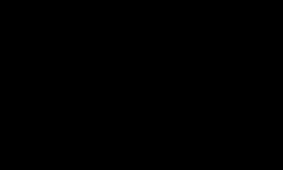
\includegraphics[width=85mm]{./imgs/im1.jpg}
\caption{\tiny{\Formular{\index{Carvalho, Ernesto de}Ernesto de Carvalho. {\slsc{Nunca é noite no mapa}} (2016)}}}

\end{figure}

O vídeo alerta para a necessidade de entendermos esses novos modelos
cartográficos a partir das ``redes'' por onde essas informações
circulam. O Google e outras empresas oferecem, aparentemente, um mapa
neutro, acessível a todos, sem a mediação subjetiva do cartógrafo. Mas
``acesso'', ou seja, aquilo que nos é oferecido ``gratuitamente'',
significa acesso àquilo que a empresa deseja nos mostrar, exatamente
como nos mapas antigos, mas agora de forma dissimulada.\footnote{Em
  1993, o fundador da Microsoft \index{Gates, Bill}Bill Gates disse, com propriedade, que
  ``a revolução digital trata de facilitação --- criar ferramentas para
  tornas as coisas fáceis'' (\scalebox{.8}{SEABROOK}, 1994, p.~48), uma afirmação que
  podemos estender ao universo dos mapas.} Conforme
``visitamos'' lugares girando o globo virtual do Google, deixamos uma
série de rastros que podem ser recuperados e usados pela empresa. E
sabemos que essas empresas de tecnologia têm seu maior patrimônio na
quantidade avassaladora de informações que coletam sobre os hábitos dos
usuários que, por sua vez, são vendidas ao mercado publicitário.
Dessa forma, a antiga vigilância panóptica é substituída pela análise
de dados que ``voluntariamente'' oferecemos a essas empresas. E, se
recordarmos as três instâncias necessárias para a existência do mapa (o
cartógrafo, a instituição e o observador), veremos que mesmo com as
novas tecnologias continuamos recebendo os mapas sem poder interferir
significativamente em sua produção.

Um dos efeitos colaterais desse novo paradigma é a transformação de
nossa sociedade de informação numa sociedade de controle e nossa cultura
visual numa cultura de vigilância. O olhar de cima para baixo,
justamente como o olhar divino, ``que tudo vê'',\footnote{O ``olho que tudo
  vê'' (ou ``olho da providência'') é o símbolo que mostra um olho
  dentro de um triângulo rodeado de raios e luzes, comumente
  interpretado como o olho de Deus vigilante sobre a humanidade.
  Representa a autoridade, a sabedoria e a onisciência. Está presente em
  várias religiões, sendo bastante associado ao cristianismo a partir do
  século \scalebox{.8}{XVIII} e à maçonaria.} desumaniza a cidade e subjuga os de
baixo com seu poder e autoridade. Já não sabemos mais se vemos ou somos
vistos, se somos sujeito ou objeto. Parece que a multiplicação dos
pontos de vista não se dá apenas em benefício do observador. Alguns
desses novos pontos de vista transformam o observador em observado. Se a
realidade era vista como que através de um buraco de fechadura,
garantindo o anonimato do observador, algo muito próximo do
\emph{voyeurismo}, agora isso pode ter se invertido.

Alguns artistas exploram criativamente essa condição, recusando a
experiência física do espaço e produzindo obras apenas para serem vistas
do alto. Aqui, a forma (como nas linhas de Nazca) não é compreensível do
nível do chão; a visão artificial, proporcionada por alguma máquina no
céu é mais importante do que o corpo no chão. Muitos artistas produzem
esse tipo de obra justamente para poder questionar as formas de
apreensão do espaço na sociedade contemporânea, marcada por vigilância e
controle visual.

O artista brasileiro \index{Lima, Daniel}Daniel Lima, em \emph{O céu nos observa} (2010),
contratou o serviço de um satélite para produzir uma fotografia da
cidade de São Paulo. A imagem de alta resolução foi agendada para às
10h30min do dia 15 de maio de 2010. Uma vez agendada a fotografia, o
artista convocou, pelas redes sociais, a todos que quisessem fazer
intervenções na cidade a fim de serem captadas pela fotografia. A
convocatória dizia que naquela dia e horário, qualquer objeto ou corpo
maior com mais de 50cm apareceria na imagem de satélite, e dava as
coordenadas da área abrangida.\footnote{O satélite passou um pouco antes
  do horário previsto, quando algumas obras ainda não estavam prontas; e
  o dia estava parcialmente nublado. Como resultado, poucas das cerca de
  25 intervenções previstas aparecem na imagem final.}

\begin{figure}[!ht]

\centering
 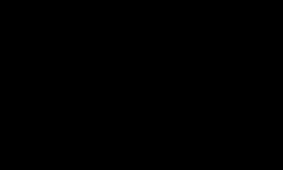
\includegraphics[width=85mm]{./imgs/im1.jpg}
\caption{\tiny{\Formular{\index{Lima, Daniel}Daniel Lima. {\slsc{O céu nos observa}} (2010)}}}

\end{figure}

Em \emph{Terra} (2017), a artista brasileira \index{Gross, Carmel}Carmela Gross cria uma
intervenção luminosa no teto da marquise do Museu Brasileiro da
Escultura. Trata"-se de uma instalação em fita de \versal{LED} azul compondo a
palavra ``\versal{TERRA}'', em alusão à célebre frase do cosmonauta russo \index{Gagarin, Yuri}Yuri
Gagarin: ``a Terra é azul''. A proposta da artista é especialmente
inquietante na medida em que a palavra em si não pode ser vista pelo
pedestre, mas a luz azul, à noite, emana um halo fantasmático sobre o
museu, indicando que algo estranho está ali.

\begin{figure}[!ht]

\centering
 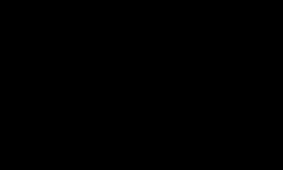
\includegraphics[width=85mm]{./imgs/im1.jpg}
\caption{\tiny{\Formular{\index{Gross, Carmel}Carmela Gross. {\slsc{Terra}} (2017)}}}

\end{figure}

Esse olhar superior, que suplanta o olhar humano ideal da perspectiva
renascentista, renova o olhar ``divino'', onisciente, autoritário e
opressor dos mapas. O suposto ``observador'' agora está flutuando no
espaço, um lugar muitas vezes inacessível ao homem comum, que passa a
criar máquinas de captação de imagem à distância. Agora já é possível
``ver'' sem ``estar''. O explorador ou o navegador, aquele que primeiro
desbravava o território, é agora aparentemente desnecessário, bastando
para isso o envio de satélites, drones, robôs e sondas não"-tripuladas
que percorrem não apenas os céus, mas também os subterrâneos da terra, o
fundo do oceano, o espaço sideral e até as entranhas do corpo.

\chapter{Navegar é preciso}

Tanto o mapa quanto a perspectiva são, no fundo, dois sistemas bastante
rígidos de representação. Do ponto de vista formal, são cortes
ortogonais da realidade visual e compartilham da mesma dificuldade de
transposição de um espaço tridimensional para uma superfície plana. O
problema da representação do espaço visual 3D na tela de pintura 2D
equivale, na cartografia, ao problema da \emph{projeção} cartográfica
--- implicando, nos dois casos, em inevitáveis distorções dos volumes.
E, a não ser que se subvertam suas regras --- como fazem muitos artistas
---, esses instrumentos em geral ignoram qualquer dimensão temporal,
mostrando o que querem mostrar de uma só vez.

Também compartilham do mesmo problema proveniente da ideia de autoridade
e de poder. Basicamente, são visões do mundo engenhosas, mas impostas de
cima para baixo. O mapa e a perspectiva têm a pretensão de separar o que
é certo do que é errado, e acreditam numa hipotética objetividade. E
mesmo que sejam sistemas diferentes entre si, padecem do mesmo mal: o
encanto da imagem. E sabemos que beleza, paixão, idolatria, cegueira e
ignorância são palavras que andam juntas. Nesse sentido, a beleza
encantadora do mapa e da perspectiva é potencialmente perigosa. Para
\index{Latour, Bruno}Bruno Latour (\versal{NOVEMBER}; \versal{CAMACHO"-HÜBNER}; \versal{LATOUR}, 2013, p.~12), será
preciso ``libertar a geografia de sua fascinação com o mapa''.

Assim como será preciso livrarmo"-nos da autoridade do mapa e recuperar
nossa capacidade de mapeamento, será preciso descartar a rigidez da
perspectiva. A solução, segundo alguns pensadores, parte do conceito
ampliado de \emph{navegação}. Tanto a prática de mapeamento quanto a de
navegação se distanciam das representações imagéticas do mapa e da
perspectiva na medida em que descartam a leitura mimética e estática do
espaço para propor uma leitura crítica baseada no movimento.

Um aspecto bastante interessante dessa proposta é ser compatível com as
novas tecnologias; o uso crítico das novas ferramentas portáteis pode,
se bem utilizadas, incrementar nossa experiência navegacional. Na
verdade, não há razão para fazer um chamado totalmente regressivo às
formas primitivas de localização espacial. Estamos caminhando para um
mundo onde os mapas impressos serão desnecessários, substituídos
inexoravelmente por mapas virtuais que se cristalizam em telas luminosas
que agora carregamos o tempo todo, como uma extensão do próprio corpo.
Numa sociedade em que as coisas estão constantemente em movimento, novas
formas de navegação como modelos tridimensionais, aplicativos,
diagramas, motores de busca e animações serão o novo paradigma.

Esses aparelhos utilizam sistemas sofisticados de localização por
satélite como \versal{GPS} (\emph{global positioning system}) e nos avisam sobre
as rotas a serem tomadas a todo instante, resultando numa situação em
que ``sabem'' mais sobre nossa localização do que nós mesmos. Com isso,
expandem o próprio significado do termo ``navegação'' e ressignificam o
primeiro impulso cartográfico, ligado às conquistas marítimas. Mas é
preciso ter cuidado. Se originalmente os instrumentos de navegação como
a bússola, o astrolábio e o sextante exigiam uma extraordinária
capacidade humana de cálculo e observação da natureza, hoje as
ferramentas de navegação nos dizem autoritariamente aonde ir e o que
fazer, inclusive emitindo ``alertas'' indesejados a todo instante,
tentando prever problemas que normalmente são solucionados naturalmente.

\begin{figure}[!ht]

\centering
 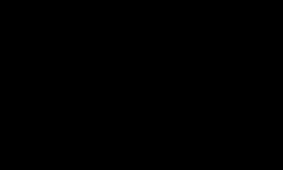
\includegraphics[width=85mm]{./imgs/im1.jpg}
\caption{\tiny{\Formular{Telas de celular com o jogo {\slsc{Pókemon \protect\scalebox{.8}{GO}}}}}}

\end{figure}

Não obstante, fazendo uso tanto da ideia de localização (posição de um objeto num sistema de coordenadas) quanto de orientação (ajuste da direção em relação aos pontos cardeais), o conceito de navegação abarca a tensão que existe
entre mapas como representações do território, e mapas como
``interfaces'' das rotas e rotinas da vida urbana. Como uma espécie de ``mapa em movimento'', a navegação pode ser
considerada uma forma central da mediação entre os espaços,
temporalidades e experiências da cidade contemporânea. Dados e informações do mundo
real estão agora frequentemente localizados no ciberespaço, sobretudo
nas plataformas de mapeamento, produzindo uma espécie de ``virtualidade
aumentada''; por outro lado, uma série de dados virtuais agora estão
localizados no espaço real, principalmente através de aplicativos de
``realidade aumentada''. Um exemplo é o jogo eletrônico \emph{Pokémon
\versal{GO}}, onde o jogador deve percorrer um lugar real guiado pelo mapa
virtual a fim de coletar prêmios, também virtuais, pelo caminho. Aqui, o
próprio jogador toma o lugar do personagem que antes controlava (como
nos jogos ao estilo \emph{Mario Bros.}) e a cidade real se torna uma
plataforma para a experiência virtual. Chama a atenção a presença desse
jogador caminhando na rua, com os olhos fixos na tela do celular, alheio
ao mundo ao redor.

Para a compreensão desses novos ambientes cartográficos, será preciso
diferenciar os usos \emph{mimético} e \emph{navegacional} do espaço,
propõe \index{Latour, Bruno}Bruno Latour (num artigo escrito em colaboração com \index{November, Valérie}Valérie
November e \index{Camacho-Hübner, Eduardo}Eduardo Camacho"-Hübner). Embora o mapa não esteja mais
confinado às duas dimensões do papel, e seja um objeto em desuso, a
``compreensão cartográfica'' do espaço está cada vez mais presente na
forma das diversas plataformas a que temos acesso. Mapas continuam
guiando nosso conhecimento acerca do que constitui o território urbano,
tanto quanto nossas atividades diárias.

Uma vez que escaparam do papel impresso que os aprisionava e alojaram"-se
nas telas luminosas, podemos considerar os mapas como painéis
(\emph{dashboards}) de uma ``interface de cálculo'' que permite ao
sujeito fazer marcações (\emph{signposts}) enquanto se movimenta pelo
espaço. Com isso, uma série de ações de antecipação, participação,
reflexividade e retroalimentação pode ser incluída na definição
navegacional dos mapas (\versal{NOVEMBER}; \versal{CAMACHO"-HÜBNER}; \versal{LATOUR}, 2013, pp.~14-21).

O advento da navegação digital faz da cartografia um ``banco de dados''
atualizado a todo instante (inclusive por nós) e a que temos acesso por
meio dessa \emph{interface} que maneja esses dados. O mapa impresso
passou a ser apenas uma entre muitas saídas (\emph{outputs}) possíveis.
Essa nova plataforma navegacional, embora revolucionária na medida em
que substitui um dos mais antigos e simbólicos artefatos científicos,
ainda compartilha com ele algumas características: a necessidade de
aquisição da informação (antes feita pela exploração do território, hoje
pela coleta de dados), o manejo dessa informação (realizado pelas
instituições ou empresas que controlam os dados), o recálculo dessa
informação (atualização dos dados), a necessidade de ``saída'' dessas
informações (como a impressão) conforme o cliente e o uso, entre outras
(2013, pp.~3-4).

A rigor, a plataforma navegacional guarda mais semelhança com os antigos
portulanos do que com os mapas tradicionais. Nesses documentos náuticos
(alguns datados do século \versal{XIII}), a representação fiel do espaço era
menos importante do que os ``dados'' necessários para a navegação. Não
havia coordenadas de latitude e longitude, mas linhas desenhadas com
auxílio do compasso e da bússola que indicavam o rumo e a distância
entre os portos, constantemente atualizadas com as informações trazidas
pelos pilotos.

As imagens que se materializavam com a colocação de pigmento sobre papel
agora se formam através de sinais luminosos. Essas novas ``imagens
virtuais'' se modificam facilmente, aparecem e desaparecem, às vezes são
armazenadas, às vezes não. Em todo caso não compartilham do desejo e da
responsabilidade que as imagens impressas carregam consigo. Imprimir
significa uma busca pela permanência, cristaliza um pensamento que se
julga definitivo, ao contrário da informação digital, passível de
apagamento a qualquer momento. Agora as imagens virtuais
``reinterpretam'' o território a todo instante, buscando correspondência
imediata com ele ``em tempo real'', como gostam de dizer os entusiastas
da tecnologia. O mapa do território onde estamos aqui e agora é aquele
que se acessa exatamente aqui e agora, condenado a se desmanchar no
instante seguinte, ao absorver novos dados e descartar os anteriores,
num permanente processo de atualização. É um mapa que acompanha nosso
movimento, e o movimento dos elementos à nossa volta, ``recalculando as
rotas'' quando necessário, desde que tenhamos acesso remoto à ``rede'',
essa entidade imaterial, que paira sobre os humanos como uma organização
\emph{cyberpunk} de um filme distópico.

Nesse sentido, por haver uma entidade que controla o fluxo de dados do
qual dependemos, discordo parcialmente do otimismo de \index{Latour, Bruno}Bruno Latour, para
quem o sistema navegacional liberta o homem da fascinação com o mapa.
Latour atribui à difusão massiva da tecnologia digital um meio de
``liberar os mapas da sua relação com uma definição espúria de
território''. De fato, a inclusão da temporalidade e do movimento na
confecção do mapa e a possibilidade de navegação por esse sistema,
retoma a ideia de percurso e mapeamento que estava na origem dos mapas
impressos, tão necessária agora. Mas, mesmo que possamos interferir na
feitura desses mapas, contribuindo com dados que podem ser incorporados
a eles, ainda há um ``sistema'' controlado por grandes empresas,
replicando o esquema das três instâncias (o cartógrafo, a instituição e
o observador) que rege a confecção dos mapas desde \index{Ptolomeu}Ptolomeu.

Em todo caso, há na proposta de sistema navegacional um potencial de
compreensão crítica do espaço que pode e deve ser usado, com possíveis
implicações políticas interessantes. Nesse sentido, deve ser considerada
como uma possível solução para o problema de ``mapeamento cognitivo''
colocado por Fredric \index{Jameson, Fredric}Jameson.

Portanto, para \index{Latour, Bruno}Latour e seus colaboradores (2013, p.~8), não só os
mapas, mas tudo aquilo que chama de ``inscrições científicas'' (figuras,
diagramas, lâminas, textos, índices, bibliografias, dicionários, animais
empalhados, tabelas, colunas, fotografias) pode ser lido de forma
\emph{mimética} (uma semelhança entre uma imagem e a sua imagem virtual)
ou \emph{navegacional} (uma conexão entre sequências de sinais
dissemelhantes). Para eles, apenas o segundo método ``pode prover
conhecimento objetivo''; o primeiro não é outra coisa que ``a
contemplação narcisista da própria imagem''. Com isso, corrobora a ideia
de que o mapeamento, ou seja, o método de apreensão do espaço a partir
do movimento, do trajeto e do percurso, é aquele que provoca a reflexão
crítica sobre o espaço.

Essa ``conexão entre sequências de sinais dissemelhantes'',
característica da experiência navegacional, se estabelece quando
prestamos atenção nas correspondências entre dois elementos sucessivos
ao longo do caminho: ``é muito mais seguro andejar de um \emph{signpost}
para o seguinte do que tentar um ousado pulo das palavras para o mundo,
dos mapas para o território'' (2013, p.~8). Seria como atravessar uma
floresta pelo alto das árvores como um macaco ou ao estilo de Tarzan,
largando um cipó apenas quando se está seguro para agarrar o outro.

\begin{figure}[!ht]

\centering
 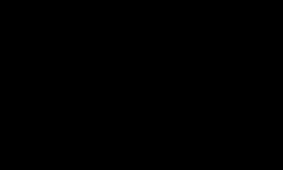
\includegraphics[width=85mm]{./imgs/im1.jpg}
\caption{\tiny{\Formular{Alinhamento de menires de Lagatjar}}}

\end{figure}

A imagem de um \emph{signpost} a cada intervalo espacial, de forma que a
partir de um se possa enxergar o outro, nos remete às mais primitivas
marcações do território. O erguimento de menires e de objetos
megalíticos semelhantes é um gesto que representa a primeira
transformação da paisagem natural num estado artificial, criando um
sistema de relações com os elementos em volta. São uma primeira atitude
de ordenação geométrica do espaço, em contraposição ao ``caos'' do mundo
natural.\footnote{Por isso, os monumentos megalíticos --- como os
  menires, dólmens e cromeleques --- estão na origem da escultura, da
  arquitetura e da paisagem, tanto no que diz respeito à construção
  física do espaço e da forma (erguimento ou o empilhamento dos
  materiais) quanto à criação de mecanismos de percepção e construção
  simbólica desse espaço (criação de percursos e delimitação abstrata do
  território). Ver \scalebox{.8}{CARERI}, Francesco. {\slsc{Walkscapes: o caminhar
    como prática estética}}. São Paulo: Gustavo Gili, 2013.}

A maioria das interpretações atribuem a esses monumentos significados
ligados ao culto ou à fertilidade. Mas, mesmo que o propósito real tenha
se perdido no tempo, resta o gesto simbólico inegável de marcação e
apropriação do território. Certamente terá servido como marco na
paisagem, um ponto de referência e de orientação territorial que se pode
ver desde certa distância, como um farol, um obelisco ou um ``pin''
virtual.

\begin{figure}[!ht]

\centering
 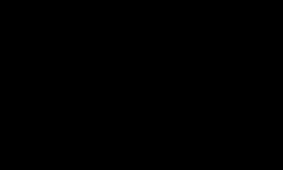
\includegraphics[width=85mm]{./imgs/im1.jpg}
\caption{\tiny{\Formular{\index{Serra, Richard}Richard Serra. {\slsc{East"-West/West"-East}} (2014)}}}

\end{figure}

O escultor norte"-americano \index{Serra, Richard}Richard Serra se utiliza desse tipo de marcação do território
como ferramenta poética em duas obras recentes de grandes dimensões. Uma
delas é \emph{Promenade} (2008), realizada para o Grand Palais, em
Paris, em que alinha, com pequenos desvios, cinco chapas de aço erguidas
verticalmente no salão do edifício. A outra é \emph{East"-West/West"-East}
(2014), instalada no deserto do Catar, com quatro placas de cerca de 15
metros de altura cada uma, alinhadas pelo topo, distribuídas numa linha
reta de um quilômetro. Nos dois casos, apesar de muito grandes
individualmente, as chapas se tornam relativamente pequenas diante da
monumentalidade do espaço onde são colocadas. Mas a distribuição precisa
pelo espaço, a tensão gerada pela sustentação e equilíbrio improváveis e
o contraste entre a ortogonalidade das peças e a natureza do ambiente em
que se encontram, criam um ``campo'' expandido que reverbera e preenche
esses imensos espaços utilizando, para isso, relativamente, muito pouco
material.

Tanto as peças de \index{Serra, Richard}Serra quanto os menires são objetos enigmáticos, cuja
simplicidade parece carregar mais sentido do que aparenta. São objetos
de grande poder simbólico, marcações inequívocas da presença do homem
sobre a Terra mas que remetem a algum tipo de força inalcançável e
espiritual.\footnote{As peças de \index{Serra, Richard}Serra lembram o enigmático monólito do
  filme {\slsc{2001 – uma odisseia no espaço}} {[}1968{]}, de \index{Kubrick, Stanley}Stanley
  Kubrick, que pode ser interpretado como a manifestação da
  inteligência, seja ela humana, artificial ou alienígena.} As obras de
\index{Serra, Richard}Serra no Catar e os alinhamentos mais complexos de menires (como em
Carnac ou em Lagatjar, na Bretanha) ``organizam a paisagem'' e podem ser
entendidos como uma a marcação de um percurso, onde cada elemento é um
\emph{signpost} que remete ao seguinte, criando linhas e demarcações de
terreno abstratas. A ligação entre dois pontos, ou seja, a reta
imaginária entre dois elementos não deixa de ser um primeiro gesto
euclidiano de marcação geométrica (literalmente ``medir a terra'') do
território que, por sua vez, vai dar origem ao mapa.


\partepigraph{Penetra surdamente no reino das palavras}{\index{Andrade, Carlos Drummond de}Carlos Drummond de Andrade, \emph{Procura da poesia} (1945)}
\part{Práticas artísticas de mapeamento}
\removeepigraph

\chapter{Arte como pergunta}

O escritor paraibano \index{Suassuna, Ariano}Ariano Suassuna, conhecido por sua obra literária
de inspiração popular, foi também professor de Estética na Universidade
Federal de Pernambuco por quase quarenta anos. Nos anos 1970 publicou o
conteúdo do curso que ministrava no livro \emph{Iniciação à estética},
que acabou servindo como uma espécie de manual --- ou livro didático ---
para seus alunos. O livro tinha como propósito --- explica o autor na
introdução --- apresentar autores e ideias cujos livros não estavam
disponíveis naquela época em Recife, ou não tinham tradução para o
português. A leitura que \index{Suassuna, Ariano}Suassuna --- um homem do nordeste tropical
brasileiro --- faz dos grandes teóricos europeus da estética, como
\index{Platão}Platão, \index{Aristóteles}Aristóteles, \index{Plotino}Plotino, \index{Tomás de Aquino}Tomás de Aquino, \index{Kant, Immanuel}Kant e \index{Hegel, Georg Wilhelm Friedrich}Hegel é, ao mesmo
tempo, rigorosa e criativa, revigorando as ideias clássicas sobre o
assunto.

Refiro"-me a \index{Suassuna, Ariano}Suassuna pois as reflexões sobre arte e sobre o Belo (como
categoria estética) que o livro traz são de um frescor raro, ao mesmo
tempo em que servem como resumo de uma linhagem de pensamento que vem
procurando definir o que é arte há muitos séculos. Tarefa inglória,
tanto porque arte é uma das atividades humanas mais difíceis de enquadrar
numa definição categórica, como porque essa mesma definição está
condenada a se transformar conforme a época, a cultura e o local. O que era arte na época de \index{Platão}Platão, por exemplo, passou a ser outra coisa para os alemães do século \textsc{xviii}. Isso para não falar da noção de arte para os povos orientais, africanos e aborígenes, entre tantas outras culturas deixadas de lado na maioria dos livros de ``história da arte''.

Podemos sempre recorrer ao léxico grego clássico e investigar o uso de
palavras como ``poiésis'', ``techné'' e ``mimesis'', ou do vocábulo
latino ``ars'', em busca de um significado latente no interior dessas
palavras. Mas, dada a distância que nos separa da Grécia Antiga, prefiro
a proposta de \index{Suassuna, Ariano}Suassuna (2005, p.~269) que, em certo momento de seu
livro, levanta uma série de perguntas provocadas pela arte, cada uma
delas relacionada a uma corrente de pensamento:

\begin{quote}
Será que a Arte tem uma origem mágica e religiosa?

Será que teve entre os povos chamados primitivos um sentido prático,
religioso e mágico, de captura do real?

Será que é uma forma de conhecimento e penetração da realidade?

Será única e exclusivamente preocupada com a criação da Beleza pura, ou
terá, pelo contrário, sempre a preocupação da utilidade prática, da
função social, da participação nos problemas sociais e na sua solução?

Será Arte toda e qualquer atividade que fabrique objetos, ou somente
aquela que se preocupa com a criação de objetos belos?

Será a Arte um modo prático, concreto e belo de tornar accessível às
massas concepções religiosas, políticas e filosóficas de natureza
abstrata?

Seria a Arte, como pretende a Estética psicanalítica, decorrente de uma
espécie de neurose, das frustrações e traumas do artista que, através
dela, procuraria, numa sublimação, se compensar da sua vida falha e
dilacerada, com a criação de um outro universo, mais belo e mais
perfeito do que o mundo real?
\end{quote}

Nessas perguntas estão expostos grande parte dos dilemas associados à
arte: como intermediária da transcendência, como ferramenta do
conhecimento e aliada da ciência, como possibilidade de ascensão
espiritual, como comunhão com a natureza (ou seu enfrentamento), como
atividade de criação de objetos úteis, como potencial de transformação
política da sociedade, como suporte principal da necessidade humana de
beleza, como veículo da comunicação de uma ideia, como solução para os
problemas humanos, para citar alguns.

Portanto, há uma grande dificuldade em encontrar uma única verdade a
respeito da natureza e da função da arte, e talvez seja melhor
aceitarmos a ideia da arte como um questionamento aberto do que
selecionar algumas definições e descartar outras conforme nosso
interesse do momento. A arte deve preservar um espaço de liberdade,
inclusive para poder negar a si própria, para corrigir seu rumo, para se
transformar com o tempo. Toda tentativa de restringir demais seu sentido
tende a ser autoritária e conservadora.

No entanto, se quisermos condensar essas preocupações num só pensamento,
podemos fazer uso da seguinte definição proposta por \index{Wisnik, Guilherme}Guilherme Wisnik
(2012b, p.~33): ``toda arte é, em última análise, uma forma de
conhecimento do mundo na qual o homem elabora materialmente a
consciência de sua condição mortal --- os mistérios da vida e da morte
---, visando, ainda que de forma indireta, mediada pela forma, construir
uma vida melhor''.

Que a arte seja uma forma de conhecimento, me parece indisputado
(\index{Suassuna, Ariano}Suassuna também se refere à expressão), e é o que faz a arte se
assemelhar à ciência e à religião em muitos aspectos. Todas essas três
criações humanas pretendem, afinal, explicar o mundo, cada uma delas à
sua maneira. Não devemos --- me parece --- perguntar qual delas oferece a
melhor explicação para uma determinada questão, mas o que cada uma delas
têm a contribuir para a compreensão dessa mesma questão. A pesquisa, a
fé e a imaginação podem ser capacidades humanas complementares, cada uma
com sua particularidade, como sugere \index{Suassuna, Ariano}Suassuna (2005, p.~274):

\begin{quote}
o papel fundamental, na criação artística, é desempenhado pela
imaginação criadora. Existe muita coisa de intelectual na criação e na
fruição da Arte; existe, mesmo, uma forma de conhecimento, na Arte, mas
é uma forma de conhecimento bastante diferente das que são exercidas
pela Ciência e pela Filosofia: é um conhecimento \emph{poético},
concreto e resultante da simples apreensão, quando a inteligência,
movida pela Beleza do que apreendeu, se põe naturalmente e sem esforço a
refletir sobre o que viu.
\end{quote}

A ideia de complementariedade é particularmente importante pois a arte
pode ocupar um espaço que a ciência e a religião não podem. Esse espaço,
como vemos em \index{Suassuna, Ariano}Suassuna, diz respeito à imaginação. Tanto o saber
científico quanto o saber empírico muitas vezes têm como motor a
capacidade de imaginação, grande responsável pelo alargamento
dos horizontes, pela extensão do campo
das possibilidades, pelas aventuras a territórios desconhecidos. A imaginação
testa os limites do pensamento humano. E uma das formas mais
interessantes de darmos vazão à imaginação é a arte, tanto no que diz
respeito à sua capacidade reativa de representar o mundo quanto de
transformá"-lo propositivamente.

Se a arte é uma forma de conhecimento, podemos fazer uso dela para nos
ajudar a solucionar alguns problemas ou explicar grandes questões
humanas quando os outros campos do conhecimento humano se encontram em
dificuldade, sobretudo quando a eles falta, justamente, imaginação. Por
exemplo: podemos explicar a invasão da Espanha por \index{Bonaparte, Napoleão}Napoleão em 1808 (ou
a guerra em si, como atividade humana), mas também mostrar a tela
\emph{Três de Maio de 1808 em Madri} (1814), de \index{Goya, Francisco de}Goya; podemos medir
proporções e harmonias, mas também podemos visitar o
Partenon em Atenas; podemos investigar fontes e estudar as Grandes
Navegações, mas também podemos ler \emph{Os Lusíadas} (1572), de \index{Camões, Luís de}Camões. Na arte, mesmo a tentativa fracassada de representar o irrepresentável tem mais valor do que a recusa dessa tentativa. De outra forma, não teríamos o \emph{Réquiem} de \index{Mozart, Wolfgang Amadeus}Mozart, o Taj Mahal, o \emph{Inferno} de \index{Alighieri, Dante}Dante e a \emph{Odisseia}, pois a morte, o amor, a divindade e a vida são todos, a rigor, pela complexidade e multiplicidade de sentidos, coisas irrepresentáveis.

Com isso, gostaria de voltar ao problema de mapeamento apontado por
Fredric \index{Jameson, Fredric}Jameson, conforme visto no primeiro capítulo. A proposta do
autor está, a rigor, mais dentro do universo da política, da economia e
da cultura do que das artes. Mas, como ele mesmo afirma, ainda não foi
possível encontrar uma forma de representação para o novo problema de
legibilidade espacial. \index{Jameson, Fredric}Jameson insiste na necessidade de
\emph{representação} do ``novo sistema mundial global'' como forma de
desalienação e aponta uma limitação para resolver esse problema dentro
do universo das ciências políticas e econômicas --- é nesse lugar que a
arte pode ser útil.

A intenção não é ilustrar diretamente o problema político e econômico
que aponta \index{Jameson, Fredric}Jameson, mas verificar se encontramos nas artes formas
originais e práticas de mapeamento que apurem nosso instinto espacial e
nos ajudem a fazer uma leitura do espaço mais crítica. A desalienação
passa pela reconquista de um sentido de localização e de reconstrução de
um espaço articulado, através de nossa capacidade de memorização.
Portanto, como vimos, é preciso \emph{recuperar} a capacidade de
mapeamento perdida. Algumas obras de arte, acredito, têm a capacidade de
nos levar de volta a essa condição perdida e provocar profundas
reflexões sobre nosso lugar no mundo. Essa busca de algo muito básico
que se perdeu é fundamental diante da velocidade das transformações
pelas quais o mundo passa --- é como recuar uma casa para avançar duas
num jogo de tabuleiro.

\chapter{Práticas artísticas de mapeamento}

Creio que podemos distinguir basicamente três práticas de mapeamento nas
artes, que utilizam estratégias distintas. Para uns, o mapeamento se
resolve como \emph{criação gráfica,} ou seja, com a realização de um
mapa propriamente; para outros o mapeamento é uma \emph{proposição
abstrata} que, em geral, exclui o mapa como objeto; e para outros é um
\emph{método de} \emph{pesquisa,} quase científico. O primeiro grupo
\emph{cria} um mapa, o segundo \emph{sugere} e o terceiro \emph{usa} o
mapa na elaboração da obra. É claro que não há como ser tão rígido
quando tratamos de arte e veremos que, na verdade, muitas obras flutuam
entre tais práticas, fazendo muitas vezes uso de mais de uma forma de
mapeamento.

Um grande número de artistas lida diretamente com o mapa como objeto
gráfico. Se, por um lado o mapa vem sofrendo uma contestação cada vez
maior no que diz respeito ao seu poder de objetividade, por outro a
capacidade de construir mundos e seu potencial poético vêm sendo
utilizados cada vez mais pelos artistas contemporâneos, sobretudo a
partir dos anos 1980.\footnote{Ver \scalebox{.8}{OBRIST}, Hans Ulrich
  (ed.). {\slsc{Mapping it out: an alternative atlas of contemporary
    cartographies}}. Londres: Thames \& Hudson, 2014; e \scalebox{.8}{HARMON}, Katharine
  (ed.). {\slsc{The map as art: contemporary artists explore
    cartography}}. Nova York: Princeton Architectural Press, 2009.} Se o mapa
tradicional, que pretende ser a representação fiel do território, não
pode mais dar conta da complexidade do mundo contemporâneo, talvez o
mapa poético, que assume sua própria subjetividade, chegue mais perto:
``mapas são importantes demais para serem delegados apenas aos
cartógrafos'', aponta \index{Harley, John Brian}John Brian Harley (1992, p.~203), um dos maiores
estudiosos do assunto.

Criar um mapa equivale a inventar um mundo. Muitos artistas se dedicaram
a criar mapas alternativos ou imaginários, ou a redesenhar os
existentes, como podemos ver no trabalho de \index{Boetti, Alighiero}Alighiero Boetti, \index{Steinberg, Saul}Saul
Steinberg, \index{Broodthaers, Marcel}Marcel Broodthaers, \index{Mir, Aleksandra}Aleksandra Mir, \index{Ferrari, León}León Ferrari, entre
tantos outros. A rigor talvez seja até difícil encontrar um artista
visual que não tenha, em algum momento de sua carreira, desenhado um
mapa ou algo parecido. Este tipo de obra pode, de fato, ser bastante
contundente, como o \emph{Mapa invertido} (1943), de \index{Torres-García, Joaquín}Joaquín
Torres"-García, uma sutil inversão cartográfica que desmonta todo um
imaginário hierárquico que, arbitrariamente, sempre colocou o Hemisfério
Norte numa posição de superioridade geográfica.

Há ainda artistas que elaboram mapas que procuram mapear justamente as
relações do mundo contemporâneo e suas implicações econômicas e
políticas, numa tentativa de representar (como quer \index{Jameson, Fredric}Jameson) toda a rede
intrincada que rege o capitalismo. Esses mapas se caracterizam por uma
enorme complexidade, por linhas de força e conexões múltiplas,
resultando num emaranhado gráfico de difícil decifração. A imagem
resultante é bastante semelhante à imagem abstrata de rede --- ou de
\emph{ciberespaço} --- que temos na mente. Em geral, contém uma crítica
ao sistema capitalista neoliberal, e tenta revelar os propósitos escusos
das grandes corporações, bancos, sistemas de governo, expondo as
conexões das redes internacionais de poder e do fluxo financeiro. Em
termos de mapa, são as obras que encaram de frente o problema da falta
de legibilidade espacial do mundo contemporâneo e se alinham às
correntes ativistas de transformação da sociedade. Podemos chamá"-las de
\emph{contracartografias}, na medida em que percebem as limitações e os
interesses de poder contidos no mapa tradicional. Ao propor um novo
mapa, propõem uma nova forma de representar o mundo que, talvez, seja
mais precisa. Assim é o trabalho do sueco"-brasileiro \index{Fahlström, Öyvind}Öyvind Fahlström,
do norte"-americano \index{Lombardi, Mark}Mark Lombardi e da dupla francesa \index{Bureau d’Études}Bureau d'Études,
por exemplo.

\begin{figure}[!ht]

\centering
 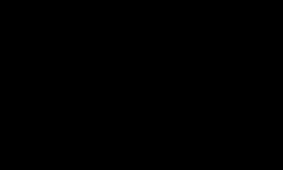
\includegraphics[width=85mm]{./imgs/im1.jpg}
\caption{\tiny{\Formular{\index{Lombardi, Mark}Mark Lombardi. {\slsc{World Finance Corporation and Associates}} (1992)}}}

\end{figure}

\begin{figure}[!ht]

\centering
 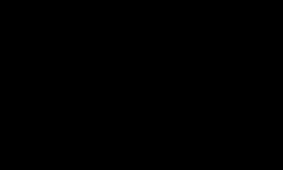
\includegraphics[width=85mm]{./imgs/im1.jpg}
\caption{\tiny{\Formular{\index{Fahlström, Öyvind}Öyvind Fahlström. {\slsc{Section of World Map – A Pluzze}} (1973). Detalhe}}}

\end{figure}

No entanto, mesmo levando em conta a contribuição inegável desses
artistas, o produto final do trabalho, mesmo que subversivo, ainda é um
mapa, que traz consigo muitos dos problemas de representação que vimos
no capítulo anterior. Como tal, é preciso aceitar a interpretação do
artista, que aqui toma o lugar do cartógrafo, assumindo a mesma posição
impositiva. Esses artistas entregam o mapa pronto, quando o que
precisamos é aprender os mecanismos de mapeamento pré"-cartográficos que,
eventualmente, podem produzir um mapa. Portanto, para esses artistas o
mapa como objeto é mais importante do que o mapeamento como conceito.

Há artistas que se relacionam com a ideia de mapa de forma indireta, às
vezes inconscientemente, como podemos ver nas pinturas da última fase de
\index{Pollock, Jackson}Jackson Pollock. Essas pinturas compartilham com o mapa o desejo de
representação gráfica de um espaço, mas um espaço mental e subjetivo,
que abriga as formas imprecisas do inconsciente. Nesse espaço instável
há uma série de fluxos, ritmos e conexões aparentemente caóticas, mas
que escondem uma lógica própria e orgânica. Isso levou \index{Argan, Giulio Carlo}Argan a associar
a pintura de \index{Pollock, Jackson}Pollock com os fluxos dos habitantes de uma cidade. Os
caminhos aparentemente aleatórios que os cidadãos percorrem diariamente,
e mesmo a experiência inconsciente de cada habitante, se representados
numa tradução gráfica de linhas e cores, resultariam num mapa muito
semelhante a um quadro de \index{Pollock, Jackson}Pollock, com seu ``emaranhado inextricável de
sinais, de traçados aparentemente arbitrários, de filamentos tortuosos,
embaraçados, que mil vezes se cruzam, se interrompem, recomeçam e,
depois de estranhas voltas, retornam ao ponto de onde partiram''
(\versal{ARGAN}, 1992, p.~231).

\begin{figure}[!ht]

\centering
 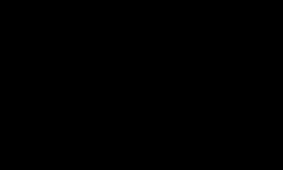
\includegraphics[width=85mm]{./imgs/im1.jpg}
\caption{\tiny{\Formular{\index{Pollock, Jackson}Jackson Pollock. {\slsc{One: Number 31, 1950}} (1950)}}}

\end{figure}

Para outros artistas, o exercício de mapeamento é mais importante e, por
isso, nos interessa mais. Nessas composições, aquele que recebe a obra (o
leitor, o espectador ou o observador) é convidado, ele próprio, a
conceber o espaço a partir da descrição ou da sugestão do autor, criando
sua própria rede de conexões espaciais. Trata"-se de uma
\emph{proposição} de mapeamento espacial. Isto vai exigir um
grande exercício de abstração por parte do receptor da obra, que acaba
construindo este espaço cognitivamente. Esta é a prática que responde
melhor à questão de Fredric \index{Jameson, Fredric}Jameson, por sua capacidade de provocar e
exigir a participação do receptor, em consonância com a atitude crítica
que o mapeamento cognitivo exige. Aqui, será preciso fazer uso de toda a
nossa capacidade de \emph{imaginação} e encontraremos um número mais
expressivo de obras na literatura e nas artes visuais.

Algumas dessas obras vão mostrando o espaço aos poucos, cabendo ao
receptor memorizar os pontos relevantes, construindo um mapa mental
gradativamente, exatamente como o rato no experimento do labirinto de
\index{Tolman, Edward}Tolman. Algumas obras produzem uma reflexão sobre o ponto de vista,
mostrando o mesmo objeto de vários ângulos. Algumas apresentam problemas
espaciais que precisam ser resolvidos, como um enigma. Há também as
obras catalográficas, que buscam exaurir conceitualmente um determinado
lugar, tentando mostrar um ``espaço total''. Há mapeamentos afetivos,
científicos, irônicos, conceituais, poéticos, inúteis, entre tantos
outros. Em geral esse tipo de proposta prescinde do mapa, ou melhor
dizendo, delega a confecção do mapa ao receptor da obra. Como resultado,
cada receptor vai conceber um mapa diferente, sujeito à própria
subjetividade, revelando a fragilidade e o autoritarismo de se propor um
mapa definitivo e único que deve ser ``obedecido'' como um livro de
leis. Não se trata mais de ``mostrar isto e não aquilo''; mas de
``mostrar o caminho para que se construa isso ou aquilo''. Encontraremos
essas proposições cartográficas, por sua vocação narrativa, em muitas
obras do cinema e da literatura, mas não apenas.

Há ainda outra prática de mapeamento, talvez a mais elementar de todas.
Trata"-se dos artistas que se utilizam do levantamento cartográfico como
ferramenta para realizar suas obras. O mapa, aqui, cumpre sua função
original de orientar espacialmente, como a um navegador no oceano ou a
um turista numa cidade desconhecida. O mapeamento não é uma proposição,
mas uma base de pesquisa --- feita pelo próprio artista ou por um
cartógrafo --- para a criação artística; a obra resulta da exploração
sistemática de um território a partir de um mapeamento realizado
previamente. O mapeamento de determinada área de interesse serve ao
artista para melhor compreendê"-la, para traçar um plano, ou lhe serve
simplesmente como inspiração, afetando o trabalho de formas distintas.
Se algumas práticas de mapeamento que vimos anteriormente têm uma
tendência ficcional, aqui estes artistas se inclinam para trabalhos de
caráter documental. Se, para alguns, é mais importante o saber da
criatividade, para estes prevalece o saber científico. No lugar da
imaginação, temos a catalogação e a pesquisa.

Uma linguagem especialmente propensa a esse tipo de método de exploração
territorial é a fotografia (sobretudo a fotografia de arquitetura). Essa
particularidade deve"-se à própria natureza do meio, que compartilha
muitas características com os mapas. Tanto fotografias quanto mapas são
representações que se pretendem objetivas, excluem o que não lhes
interessa, aproximam o que está distante, reduzem as dimensões do mundo,
transformam o tridimensional em bidimensional, possuem um autor,
congelam o tempo, são instrumentos da ciência, da arte e do poder, são
documentos, compartilham o mesmo tipo de suporte (papel ou digital), são enigmáticos e atraentes. O ato de fotografar um
lugar muitas vezes já é uma forma de mapeamento do espaço, como nos
trabalhos de \index{Atget, Eugène}Eugène Atget, \index{Azevedo, Militão Augusto de}Militão Augusto de Azevedo, \index{Ruscha, Ed}Ed Ruscha e do
casal \index{Becher, Bernd e Hilla}Becher, por exemplo.\footnote{Além da prática de mapeamento, e do
  uso da fotografia como linguagem e suporte, alguns desses artistas têm
  em comum --- uma vez que o mapa remete sobretudo ao espaço físico --- um
  interesse especial pelo espaço urbano e pela arquitetura. A relação
  entre fotografia e arquitetura é de mão dupla. Por um lado, a
  arquitetura está presente na fotografia desde sua invenção (havia a
  conveniência técnica de ser um motivo imóvel para poder ser registrado
  nos primeiros materiais fotossensíveis, que exigiam longos tempos de
  exposição) e sempre foi um dos motivos fotográficos mais importantes.
  Por outro lado, a arquitetura é influenciada enormemente pela
  fotografia. Para \index{Solà-Morales, Ignasi de}Solà"-Morales (2002, p.~181), ``a imagem da
  arquitetura é uma imagem mediatizada que, segundo os recursos da
  representação plana da fotografia, nos facilita o acesso e a
  compreensão do objeto''.}

\begin{figure}[!ht]

\centering
 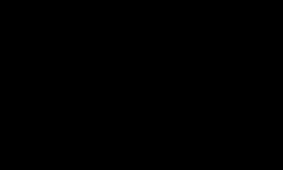
\includegraphics[width=85mm]{./imgs/im1.jpg}
\caption{\tiny{\Formular{\index{Torres-García, Joaquín}Joaquín Torres"-García. {\slsc{Mapa invertido}} (1943)}}}

\end{figure}

\chapter{Labirintos}

A obra de \index{Kafka, Franz}Kafka é uma das mais estudadas do século passado, com uma
bibliografia crítica que chega aos milhares de textos. No entanto, as
muitas tentativas dos estudiosos de decifrar os enigmas da obra kafkiana
sempre foram insuficientes. Interpretações teológicas, hermenêuticas,
comparativas, estéticas, históricas e biográficas tentaram revelar o
que está por trás de seus escritos, de seu universo alegórico e
simbólico, sem nunca chegar a um termo satisfatório.

No entanto, através da reverberação de sua literatura em outros
escritores podemos vislumbrar muito de sua técnica e delimitar um campo
de interpretação. Um escritor experimenta as dificuldades do outro
escritor e, pela comparação, podemos entrever alguns problemas que regem
a criação literária. Interpretações bastante originais da obra de \index{Kafka, Franz}Kafka
podem ser encontradas na obra de escritores que por ele foram
influenciados como \index{Camus, Albert}Albert Camus, \index{Buzzati, Dino}Dino Buzzati, \index{Calvino, Italo}Italo Calvino, \index{Saramago, José}José
Saramago e \index{Borges, Jorge Luis}Jorge Luis Borges, para citar alguns. Esses escritores
souberam aceitar o enigma que a obra de \index{Kafka, Franz}Kafka propõe e muitas vezes
trouxeram assumidamente para suas próprias obras essa influência,
fazendo com que o leitor atento a reconheça e muitas vezes a compreenda
melhor. Muitas vezes o entendimento --- e o prazer dele decorrente --- é
resultado da aceitação da beleza de um enigma, e não de sua solução. Os
símbolos kafkianos e sua obscuridade talvez possam ser melhor entendidos
ou melhor visualizados (nunca decifrados) quando lemos Jorge Luis
\index{Borges, Jorge Luis}Borges, por exemplo. Borges vai lançar uma luz sobre a obra do tcheco
que, se não ilumina completamente seus textos, ao menos delimita o campo
onde se inserem seus signos.\footnote{\index{Borges, Jorge Luis}Borges era grande admirador de
  \index{Kafka, Franz}Kafka, traduziu para o espanhol algumas de suas obras e escreveu
  textos sobre ele. Num deles chega a afirmar que ``Kafka es el gran
  escritor clásico de nuestro atormentado y extraño siglo'' (\scalebox{.8}{BORGES},
  2007c, p.~555). É autor de um curto ensaio, {\slsc{Kafka y sus
    precursores}}, onde identifica num dos paradoxos de \index{Zenão de Eleia}Zenão a origem da
  condição kafkiana e o angustiante movimento ao infinito que persegue
  seus personagens. Neste ensaio, \index{Borges, Jorge Luis}Borges também postula que \index{Kafka, Franz}Kafka é um
  escritor tão poderoso a ponto de modificar a leitura de seus
  precursores como se, depois de Kafka, a obra desses escritores fosse
  ``afinada e desviada'' por sua influência: ``su labor modifica nuestra
  concepción del pasado, como ha de modificar el futuro'' (\scalebox{.8}{BORGES},
  2007b, p.~107).}

No prefácio que escreve para uma edição de \emph{A metamorfose}, o
escritor argentino é bastante claro: ``la elaboración, en \index{Kafka, Franz}Kafka, es
menos admirable que la invención (\ldots{}). El argumento y el ambiente son
lo esencial'' (\versal{KAFKA}, 2001, p.~11). No prefácio a uma edição inglesa de
\emph{O processo}, \index{Borges, Jorge Luis}Borges elege seus textos preferidos de \index{Kafka, Franz}Kafka, entre
eles \emph{Uma mensagem imperial}, \emph{Diante da lei} e, sobretudo,
\emph{Durante a construção da muralha da China}, onde aparecem dois
signos importantes que vão frequentar também a obra de \index{Borges, Jorge Luis}Borges: o
infinito e o labirinto.

O labirinto, tanto em \index{Borges, Jorge Luis}Borges quanto em \index{Kafka, Franz}Kafka, terá um significado
metafísico. Podemos encontrar em \index{Borges, Jorge Luis}Borges muitas definições, mas todas
partem do pressuposto de que ``un laberinto es una casa labrada para
confundir a los hombres; su arquitectura, pródiga en simetrías, está
subordinada a esse fin'' (2007a, p.~647). E explica sua preferência pelo
tema: ``yo, para expresar esa perplejidad que me ha acompañado a lo
largo de la vida y que hace que muchos de mis propios actos me sean
inexplicables, elegí el símbolo del laberinto o, mejor dicho, el
laberinto me fue impuesto, porque la idea de un edificio construido para
que alguien se pierda, es el símbolo inevitable de la perplejidad''
(1988, p.~79).

O labirinto se relaciona com a arquitetura de forma conflitante --- ele é
e não é arquitetura ao mesmo tempo. É um edifício, mas também se opõe à
ideia de arquitetura (e do urbanismo moderno) que tem, entre suas
funções, justamente evitar a desorientação. E, se o labirinto pode ser
definido como uma construção caracterizada por caminhos e bloqueios cuja
totalidade nos é negada, e cuja finalidade é a desorientação, não é
difícil estender essa experiência para a própria experiência da cidade e
do mundo. Afinal, qual a diferença entre o labirinto de Cnossos e a
experiência de caminhar numa cidade de ruas sinuosas ou mesmo numa
megacidade contemporânea?\footnote{O labirinto mitológico de Cnossos foi
  encomendado pelo rei Minos ao arquiteto \index{Dedalo@Dédalo}Dédalo para aprisionar o
  Minotauro. A lenda conta que o herói Teseu se dispôs a entrar no
  labirinto para enfrentar o monstro. Conforme entrava no labirinto,
  Teseu desenrolava um fio dado a ele pela amada Ariadne e assim, depois
  de matar o Minotauro, pôde encontrar o caminho de volta.} Assim, o
labirinto é uma poderosa metáfora de nossa condição como cidadão do
mundo: ``no precisa erigir un laberinto, cuando el universo ya lo es''
(\versal{BORGES}, 2007a, p.~727).

\begin{figure}[!ht]

\centering
 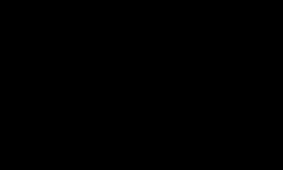
\includegraphics[width=85mm]{./imgs/im1.jpg}
\caption{\tiny{\Formular{\index{Ferrari, León}León Ferrari. {\slsc{Cidade}} (1980)}}}

\end{figure}

Na \emph{Parábola del palacio}, \index{Borges, Jorge Luis}Borges (2007, v.~\versal{II}, p.~214) fala de um
labirinto tão grande que parece abarcar todo o mundo com seus jardins
esplendorosos, avenidas, bibliotecas, rios e ilhas: ``parecía imposible
que la tierra fuera otra cosa que jardines, aguas, arquitecturas y
formas de esplendor''. Ora, se o labirinto é o tamanho do mundo, das
duas, uma: ou ele deixa de ser um labirinto (pois elimina as noções de
dentro, fora, preso e livre), ou precisamos entender o mundo como um
grande labirinto. Talvez seja esse o motivo da grande fascinação que
essa construção paradoxal exerce, pois podemos entender o labirinto como
uma grande metáfora do mundo dentro do qual estamos presos, e do qual
não há saída.

O labirinto implica duas percepções bastante distintas: de fora e de
dentro, ou seja, uma passiva e distante, como um mapa, outra
fenomenológica e imersiva, que testa nossa capacidade de mapeamento (uma
situação brilhantemente ilustrada no filme \emph{O iluminado} [1980], de
\index{Kubrick, Stanley}Stanley Kubrick). A primeira imagem que nos vem à mente é sempre o
labirinto visto do alto, como numa fotografia aérea ou num desenho. Mas
para que a verdadeira experiência labiríntica se configure, é essencial
a imersão no espaço desconhecido, é preciso que não se conheça o mapa
(um instrumento de orientação) do labirinto (uma construção
desorientadora). O paradoxo consiste em que o mapa do labirinto, ao
revelar sua solução, anula a experiência labiríntica cuja angústia vem
da incerteza, da experiência fragmentada, do fato de não se saber onde
está, de estar sempre no meio.

\begin{figure}[!ht]

\centering
 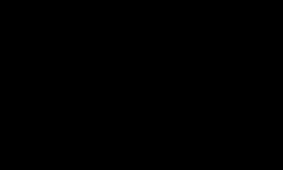
\includegraphics[width=85mm]{./imgs/im1.jpg}
\caption{\tiny{\Formular{\index{Kubrick, Stanley}Stanley Kubrick. {\slsc{O iluminado}} (1980)}}}

\end{figure}

Justamente, nos labirintos de \index{Borges, Jorge Luis}Borges e \index{Kafka, Franz}, a experiência subjetiva do
labirinto é mais importante que a construção em si. Em outras palavras,
não basta a descrição do labirinto para se experimentar a perplexidade
de que fala \index{Borges, Jorge Luis}Borges. Esses escritores sabem que a situação labiríntica
não depende apenas de paredes e escadas, depende de bloqueios e acessos
de outra ordem. A experiência do labirinto se dá não apenas
espacialmente, mas também temporalmente. O labirinto é o equivalente
espacial do infinito, assim como o infinito é o equivalente temporal do
labirinto. No universo literário desses escritores o infinito e o
labirinto muitas vezes caminham juntos como metáforas essenciais do
tempo e do espaço.

Vejamos como esses autores tratam do tema:

\begin{quote}
\forceindent{}\versal{UMA MENSAGEM IMPERIAL}

O imperador --- assim consta --- enviou a você, o só, o súdito lastimável,
a minúscula sombra refugiada na mais remota distância diante do sol
imperial, exatamente a você o imperador enviou do leito de morte uma
mensagem. Fez o mensageiro se ajoelhar ao pé da cama e segredou"-lhe a
mensagem no ouvido; estava tão empenhado nela que o mandou ainda
repeti"-la no seu próprio ouvido. Com um aceno de cabeça confirmou a
exatidão do que tinha sido dito. E perante todos os que assistem à sua
morte --- todas as paredes que impedem a vista foram derrubadas e nas
amplas escadarias que se lançam ao alto os grandes do reino formam um
círculo --- perante todos eles o imperador despachou o mensageiro. Este
se pôs imediatamente em marcha; é um homem robusto, infatigável;
estendendo ora um, ora outro braço, ele abre caminho na multidão; quando
encontra resistência aponta para o peito onde está o símbolo do sol;
avança fácil como nenhum outro. Mas a multidão é tão grande, suas
moradas não têm fim. Fosse um campo livre que se abrisse, como ele
voaria! --- e certamente você logo ouviria a esplêndida batida dos seus
punhos na porta. Ao invés disso, porém --- como são vãos os seus
esforços; continua sempre forçando a passagem pelos aposentos do palácio
mais interno; nunca irá ultrapassá"-los; e se os conseguisse, nada
estaria ganho; teria de percorrer os pátios de ponta a ponta e, depois
dos pátios, o segundo palácio que os circunda; e outra vez escadas e
pátios; e novamente um palácio; e assim por diante, durante milênios; e
se afinal ele se precipitasse do mais externo dos portões --- mas isso
não pode acontecer jamais, jamais --- só então ele teria diante de si a
cidade"-sede, o centro do mundo, repleto pela própria borra amontoada.
Aqui ninguém penetra; muito menos com a mensagem de um morto. --- Você no
entanto está sentado junto à janela e sonha com ela quando a noite
chega (\versal{KAFKA}, 2001, p.~41).
\end{quote}

Nesta parábola\footnote{A parábola é uma narrativa curta e simples
  que, através de analogias, contém uma mensagem de cunho didático ou
  moral. É muito presente em textos espirituais como a Bíblia,
  notadamente nas pregações de Jesus.} de \index{Kafka, Franz}Kafka, o labirinto não é expresso, nem mesmo essa
palavra é usada. Ele é sugerido pois, para Kafka o
labirinto, ou a situação labiríntica, está em toda parte e todos os
homens estão dentro dele --- é o próprio mundo. \index{Kafka, Franz}Kafka constrói esse
espaço infinito ao longo da narrativa, acrescenta escadas e pátios à
medida que o mensageiro avança. Constrói através das palavras:
``paredes'', ``impedem'', ``vista'', ``escadarias'', ``círculo'',
``marcha'', ``infatigável'', ``caminho'', ``resistência'', ``avança'',
``campo'', ``esforços'', ``continua'', ``passagem'', ``aposentos'',
``palácio'', ``interno'', ``nunca'', ``percorrer'', ``pátios'', ``ponta
a ponta'', ``pátios'', ``segundo palácio'', ``circunda'', ``escadas'',
``pátios'', ``palácio'', ``milênios''. O labirinto de \index{Kafka, Franz}Kafka não tem 
saída ou se tem (``mas isso não pode acontecer jamais, jamais''), o
mundo de fora pode ser ainda pior. A angústia é dupla: ao
descrever a situação do mensageiro imerso no labirinto (a experiência
fenomenológica de quem está dentro do labirinto sem conhecer seu mapa)
e ao postergar infinitamente a entrega da mensagem. Arriscando ainda um
pouco mais, podemos dizer que esse labirinto de \index{Kafka, Franz}Kafka não tem saída pois
a saída do labirinto metafísico pressupõe uma intervenção divina ou
transcendente.

Vejamos agora como \index{Borges, Jorge Luis}Jorge Luis Borges trata do tema do labirinto, nesta
parábola aparentemente saída do \emph{Livro das mil e uma noites}:

\begin{quote}
\forceindent{}\versal{LOS DOS REYES Y LOS DOS LABERINTOS} \label{borges}

Cuentan los hombres dignos de fe (pero Alá sabe más) que en los primeros
días hubo un rey de las islas de Babilonia que congregó a sus
arquitectos y magos y les mandó a construir un laberinto tan perplejo y
sutil que los varones más prudentes no se aventuraban a entrar, y los
que entraban se perdían. Esa obra era un escándalo, porque la confusión
y la maravilla son operaciones propias de Dios y no de los hombres. Con
el andar del tiempo vino a su corte un rey de los árabes, y el rey de
Babilonia (para hacer burla de la simplicidad de su huésped) lo hizo
penetrar en el laberinto, donde vagó afrentado y confundido hasta la
declinación de la tarde. Entonces imploró socorro divino y dio con la
puerta. Sus labios no profirieron queja ninguna, pero le dijo al rey de
Babilonia que él en Arabia tenía otro laberinto y que, si Dios era
servido, se lo daría a conocer algún día. Luego regresó a Arabia, juntó
sus capitanes y sus alcaides y estragó los reinos de Babilonia con tan
venturosa fortuna que derribo sus castillos, rompió sus gentes e hizo
cautivo al mismo rey. Lo amarró encima de un camello veloz y lo llevó al
desierto. Cabalgaron tres días, y le dijo: ``Oh, rey del tiempo y
substancia y cifra del siglo!, en Babilonia me quisiste perder en un
laberinto de bronce con muchas escaleras, puertas y muros; ahora el
Poderoso ha tenido a bien que te muestre el mío, donde no hay escaleras
que subir, ni puertas que forzar, ni fatigosas galerías que recorrer, ni
muros que veden el paso''.

Luego le desató las ligaduras y lo abandonó en la mitad del desierto,
donde murió de hambre y de sed. La gloria sea con Aquel que no muere
(\versal{BORGES}, 2007a, p.~731).\footnote{O texto foi publicado pela primeira
  vez em junho de 1939 na revista {\slsc{El Hogar}}, intitulado {\slsc{Una
    leyenda arábiga.}} Era atribuído (falsamente) ao explorador inglês \index{Burton, Sir Richard Francis}Sir
  Richard Francis Burton e trazia uma introdução: ``De las notas que
  Burton agregó a su famosa traducción del libro {\slsc{Las mil y una
    noches}}, traslado esta curiosa leyenda. Se titula: `Historia de los
  dos reyes y los dos laberintos`''. A parábola depois foi incorporada
  ao livro {\slsc{El Aleph}} (1949) e trazia a seguinte nota: ``Ésta es la
  historia que el rector divulgó desde el púlpito. Veáse la página
  601'', remetendo a um outro conto do mesmo livro. No epílogo do livro,
  o autor ainda explicava que ``los copistas intercalaron en {\slsc{Las mil y
  una noches}} y que omitió el prudente Galland''. Há ainda outros
  comentários em outras edições. Atribuições falsas, pseudônimos,
  intertextos, autores inventados, remissões e citações são elementos
  importantes na obra de \index{Borges, Jorge Luis}Borges. Com isso, ele acrescenta uma série de
  nomes à sua já vasta coleção de escritores preferidos e que cita
  regularmente, confundindo o leitor. Para o leitor, é difícil fazer a
  distinção, uma vez que desconhece muitas vezes tanto os autores
  conhecidos quanto os inventados. Assim, a própria erudição de \index{Borges, Jorge Luis}Borges,
  inalcançável para a maioria de nós, acaba criando uma permanente
  atmosfera de indeterminação, uma obra em camadas, um ``labirinto''
  literário onde muitas vezes não sabemos quem escreve nem de onde
  surgiu o texto. Dessa forma, \index{Borges, Jorge Luis}Borges se coloca como se fosse apenas um
  intermediário entre a literatura e o leitor, retirando de si a
  responsabilidade pelo texto, mas dando autoridade a ele. Além de
  escritor, \index{Borges, Jorge Luis}Borges foi um grande ``reescritor'' da literatura.}
\end{quote}

Em \emph{Los dos reyes y los dos laberintos}, a palavra labirinto se
repete cinco vezes. Há um rei que determina a construção do um
labirinto, construtores (``arquitectos y magos'') que realizam a tarefa
de forma que o espaço do labirinto seja palpável. Aqui ela é mais
``real'' do que em \index{Kafka, Franz}Kafka, com seus limites determinados, mas conserva
sua significação metafísica. Se Kafka constrói com palavras, \index{Borges, Jorge Luis}Borges
constrói (no primeiro labirinto do texto) com ``muchas escaleras,
puertas y muros''. Se \index{Kafka, Franz}Kafka descreve a experiência de estar dentro do
labirinto, \index{Borges, Jorge Luis}Borges adota uma perspectiva panorâmica.

Por definição, o labirinto é um espaço determinado e circunscrito
(portanto finito), cujo percurso interno é potencialmente infinito. Se o
espaço interno é o lugar do aprisionamento, o espaço exterior é o espaço
da liberdade. No entanto, \index{Borges, Jorge Luis}Borges fala de dois labirintos. O primeiro é
um projeto arquitetônico e racional, produto da vontade e engenho do
homem. O segundo é o deserto, portanto a ausência total de projeto. Se a
função primeira do labirinto é fazer com que o indivíduo se perca, o
deserto é, de certa forma, o labirinto perfeito, pois cumpre essa função
com muito mais simplicidade. É um labirinto sem entrada e, portanto, sem
saída, um lugar que não se modifica com o deslocamento. Qualquer caminho
tomado levará novamente ao meio do deserto.\footnote{Se existisse um
  mapa desse labirinto, seria uma folha em branco como o mapa de
  Bellman. Ver página~\pageref{bellman}.}

O rei da Babilônia constrói um labirinto que é um ``escândalo''
tentando, dessa forma, se aproximar de Deus ou ser como Deus, ignorando
que ``la confusión y la maravilla son operaciones propias de Dios y no
de los hombres''. Sabemos que uma ideia comum a muitas religiões prega a
simplicidade como forma de sabedoria (que se afirma na própria imagem do
deserto). No texto de \index{Borges, Jorge Luis}Borges, o homem alcança a revelação através da
consciência de sua inferioridade diante do divino. O rei da Arábia que
se perde no labirinto é um homem simples, que não se propõe a resolver o
enigma e pede humildemente ajuda a Deus. Não há dúvida de que a saída do
labirinto é uma concessão de Deus que se dá somente depois que o homem
reconhece suas próprias limitações. Deus não só ajuda o rei da Arábia a
sair do labirinto, como também o ajuda a se ``vingar'' do rei da
Babilônia. Melhor dizendo, não se trata exatamente de vingança, e sim de
justiça divina.

Se a figura de Deus está presente em \index{Borges, Jorge Luis}Borges como força redentora e fonte
da sabedoria, ela é extremamente obscura na obra de \index{Kafka, Franz}Kafka, onde a
autoridade é sempre repressora. Se a participação no próprio mundo que
nos rodeia já nos é negada, participar do universo e de Deus é além do
impossível. \index{Kafka, Franz}Kafka prefere colocar seus personagens embaixo da terra
(\emph{A construção}) ou transformá"-los num inseto (\emph{A
metamorfose}) a aproximá"-los de Deus.

Em \emph{Uma mensagem imperial}, o mensageiro simboliza a única
possibilidade de contato entre o imperador (o poder) e o povo (nós). Mas
a distância e o tempo para percorrê"-la se torna tão grande que provoca
uma ruptura: já não é mais possível unir as pontas. Já nem importa mais
se o imperador está vivo (ou se realmente existe), nem o conteúdo da
mensagem. A missão impossível do mensageiro deixa de ser uma condição
provisória, que teria um fim, para ser a condição permanente e
angustiante da existência. O escritor norte"-americano \index{Wallace, David Foster}David Foster
Wallace (2012, p.~235) sintetiza com precisão essa grande e terrível
ironia kafkiana ``de que o esforço terrível de estabelecer um
\emph{self} humano resulta num \emph{self} cuja humanidade é
indissociável desse esforço terrível. De que a jornada interminável e
impossível rumo ao nosso lar é, na verdade, o nosso lar''.

O único alento aparente para o mensageiro reside em sua própria
ignorância. Ele traz no peito o símbolo do sol, que ao mesmo tempo
permite o avanço e o coloca em seu lugar de inferioridade. Ele acredita,
inutilmente, na importância de sua missão e pretende cumpri"-la com
dedicação. Mas essa ignorância é o que prolonga sua agonia, criando a
situação tipicamente kafkiana, onde a permanência da angústia é mais
opressora que a própria morte. Algo, seja um ``fio de esperança'', seja
uma incapacidade, sempre impede que os personagens de \index{Kafka, Franz}Kafka possam optar
pela própria morte. Em outras palavras, nem mesmo a sua própria vida
lhes pertence.

Se \index{Kafka, Franz}Kafka ao menos oferece ao mensageiro o lugar da ignorância, reserva o
mais angustiante dos lugares ao leitor, essa ``a minúscula sombra
refugiada na mais remota distância diante do sol imperial''. Se o
mensageiro é uma terceira pessoa (``Er'', de quem se fala), o leitor
está no lugar da segunda (``Du'', a quem se dirige a fala). O narrador
se dirige diretamente ao leitor e é capaz inclusive de ler seus
pensamentos. Portanto, esse leitor tem consciência de que a mensagem que
lhe está destinada nunca chegará e, se chegar, já não terá nenhuma
utilidade.

Segundo o próprio \index{Borges, Jorge Luis}Borges (2007d, p.~117), a obra de \index{Kafka, Franz}Kafka é regida por
duas ideias (ou ``obsessões''): a subordinação e a postergação infinita.
Na infinitude do labirinto kafkiano, não haverá salvação divina. Estamos
na base mais profunda de uma hierarquia opressora e infinita, cujo alto
está tão distante a ponto de ser completamente inacessível. Kafka não se
refere nem mesmo à figura de Deus, pois o indivíduo é incapaz de
suportar mesmo o poder dos intermediários que estão imediatamente acima
dos homens. Se Deus existe em \index{Kafka, Franz}Kafka, nem mesmo seu nome pode ser
pronunciado.

Se em \emph{Uma mensagem imperial} o mensageiro tenta sair, mas não
consegue, num outro conto de \index{Kafka, Franz}Kafka o personagem conhece a saída, mas
prefere permanecer dentro do labirinto. Em \emph{A construção} (1923) \label{construcao}
esse personagem é uma criatura subterrânea, inquieta, que passa os dias
vistoriando e aprimorando a rede de túneis, passagens e salões onde
vive. A criatura conta com essa estrutura arquitetônica para sua própria
defesa, armazenando alimento e traçando rotas de fugas diante de um
perigo que pode vir de fora, sempre iminente, criando um ambiente de
permanente angústia.

O conto é narrado em primeira pessoa, colocando o leitor no lugar dessa
criatura paranoica, percorrendo e construindo o labirinto junto dela. Com
isso, o leitor também vai se familiarizando com o espaço, exatamente
como o rato de laboratório no labirinto de \index{Tolman, Edward}Tolman. Trata"-se precisamente
da modalidade mais primitiva de mapeamento cognitivo, ou seja, memorizar
um território à medida que o percorremos, com base em pontos de
referência mais marcantes. Ao nos colocar no lugar do animal, ``lendo''
um espaço motivado pela própria sobrevivência, \index{Kafka, Franz}Kafka nos lembra que o
mapeamento cognitivo é uma questão de vida ou morte.

Se o medo está diretamente ligado ao desconhecido, o espaço mapeado
oferece segurança, diferentemente do mundo exterior, onde a criatura
fica desprotegida. Por isso, cuidar da qualidade e da eficiência desse
espaço labiríntico e claustrofóbico significa cuidar da própria vida.
Mas isso é tão trabalhoso e crucial que a criatura se isola
completamente. O labirinto construído passa a ser seu próprio mundo, o
único que pode parcialmente dominar, ainda que a um custo muito alto.

Podemos enxergar nesse conto de \index{Kafka, Franz}Kafka a ilustração de um falso dilema da
legibilidade do espaço, segundo o qual quanto menor é o espaço, mais
fácil é seu mapeamento. No entanto, dois problemas são levantados: o
espaço menor exige uma minúcia maior, onde cada detalhe se torna muito
importante; e quanto mais mapeamos apenas um espaço restrito\emph{,}
mais o espaço exterior se torna hostil. No universo kafkiano, a saída do
labirinto não é a solução, mas o verdadeiro problema. O labirinto não é
apenas o lugar onde não se deve entrar; pode ser também o lugar de onde
não se deve sair.

\emph{Uma mensagem imperial} foi publicado separadamente, mas é um
fragmento de outro conto de \index{Kafka, Franz}Kafka chamado \emph{Durante a construção da
muralha da China}, o favorito de Jorge Luis \index{Borges, Jorge Luis}Borges. Esta desoladora
narrativa é um texto fragmentado a inacabado --- como muitas obras de
\index{Kafka, Franz}Kafka --- que fala da interminável construção de uma muralha de defesa
num império remoto. No texto, em vez de construir a muralha de forma
contínua, os construtores optam por erguê"-la em fragmentos para depois
tentar preencher os espaços entre eles. Há grandes lacunas, diferentes
materiais e trechos já em ruínas, tornando a obra inacabada e inútil em
sua função de defesa.

O empreendimento é tão gigantesco que nenhum indivíduo tem uma visão
geral da obra, nem mesmo o imperador, isolado em seu palácio e afastado
do povo, como vimos (em determinado momento, o narrador interrompe o
relato e conta a lenda do mensageiro como forma de ilustrar a relação
entre o povo e o imperador). Apenas o ``comando'', o verdadeiro
empreendedor da obra, poderia dar alguma resposta, mas é uma entidade
misteriosa e inatingível, instância superior de onde emana o verdadeiro
poder que determina o destino dos homens e da sociedade.

A obra de \index{Kafka, Franz}Kafka exige e repele interpretações ao mesmo tempo. É sempre
arriscado tentar decifrar as verdadeiras intenções do autor. Mas, ao
mesmo tempo, é difícil não enxergar uma poderosa metáfora do poder
nessas instâncias superiores, que aparecem em várias de suas obras, como
\emph{O castelo} e \emph{O processo}. Assim, trazendo as imagens criadas
por \index{Kafka, Franz}Kafka para o mundo contemporâneo, podemos pensar no ``comando'' como
uma representação das instâncias de poder ligadas ao capital às quais
não temos nenhum acesso, mas que determinam na prática o funcionamento
de nossa sociedade. Afinal, são eles que possuem os recursos financeiro
para a obra, gerenciam seu funcionamento e contratam os trabalhadores.
Podemos também pensar no imperador, alheio a tudo em seu palácio, como a
personificação de um frágil poder simbólico e político que, na prática,
está submetido a esse poder do capital.

Por sua vez, a impossibilidade de ``mapear'' a totalidade da muralha por
parte do indivíduo seria análoga à nossa incapacidade de mapear
cognitivamente o novo espaço contemporâneo, fragmentado e disperso, com
todas suas complexidades. No texto, quando um grupo de trabalhadores
termina um trecho da muralha, este mesmo grupo é enviado para regiões
distantes, impedindo que tenham uma visão do conjunto da obra. Portanto,
mais do que uma impossibilidade inerente, este seria um projeto
deliberado de debilitação de nossa capacidade de mapeamento, pois o
monopólio do mapa e do controle do espaço (exclusividade do ``comando'')
é requisito fundamental para qualquer projeto de poder.

\index{Candido, Antonio}Antonio Candido enxerga uma relação entre o enredo de \emph{Durante a
construção da muralha da China}, onde se constrói a muralha a partir de
trechos desconectados e espalhados pelo império, com o próprio modo
fragmentário e descontínuo da produção literária de \index{Kafka, Franz}Kafka, com seus
romances inacabados, parábolas curtas, manuscritos soltos, aforismos e
publicações esparsas. \index{Candido, Antonio}Candido sugere que a própria ideia de completude e
acabamento está excluída da obra de \index{Kafka, Franz}Kafka.\footnote{Ver \scalebox{.8}{CANDIDO},
  Antonio, ``Na muralha'', in {\slsc{O discurso e a cidade}}. São Paulo:
  Duas Cidades, 1993, p.~163.}

Entendo que mais do que inacabadas, suas obras são ``inacabáveis'', uma
condição que favorece a própria tensão da narrativa kafkiana. Parte da
angústia que sentimos diante da leitura de \index{Kafka, Franz}Kafka vem justamente da
ausência de solução e de desfecho na maioria de seus textos, sendo eles
terminados ou não. Em alguns, nem mesmo a morte do personagem, que
poderia colocar um fim nesta angústia, é oferecida como alívio. Em
\emph{Durante a construção da muralha da China}, a própria muralha é
impossível de ser terminada, podendo ser entendida não apenas como uma
metáfora do infinito, mas de vários infinitos simultâneos, como observou
\index{Borges, Jorge Luis}Borges: ``para detener el curso de ejércitos infinitamente lejanos, un
emperador infinitamente remoto en el tiempo y en el espacio ordena que
infinitas generaciones levanten infinitamente un muro infinito que dé la
vuelta a su imperio infinito'' (\versal{KAFKA}, 2001, p.~10). Essa
impossibilidade, que está presente no enredo de muitos textos de \index{Kafka, Franz}Kafka
como esse, está presente também na estrutura de sua obra. Muitos textos
foram deixados pelo autor como fragmento, sem ponto final, deixando em
suspenso qualquer desfecho alentador.

Se inacabada é a obra que não foi terminada por causa da morte do autor,
mas cuja completude é vislumbrada, inacabável é a obra que jamais
chegará a seu fim, que faz de sua condição incompleta e de sua
``infinitude'', uma virtude. Assim é a enigmática pintura \emph{A noiva
despida por seus celibatários, mesmo} (1915-1923), de \index{Duchamp, Marcel}Marcel
Duchamp, mais conhecida como \emph{O grande vidro}, declarada
``permanentemente inacabada'' em 1923, oito anos após ter sido iniciada.
Ou a série fotográfica \emph{Pessoas do século \versal{XX}}, (1911-1945), de
\index{Sander, August}August Sander, em sua tentativa de catalogar a fisionomia humana de seu
tempo. Poderíamos incluir nessa categoria o projeto original de
\index{Michelangelo}Michelangelo para o túmulo do papa Júlio \versal{II}, o \emph{Atlas Mnemosyne}
(1927-1929), de \index{Warburg, Aby}Aby Warburg, muitas catedrais góticas, boa parte da obra
de \index{Rodin, Auguste}Auguste Rodin e, talvez, a mítica \emph{Uma história oral de nosso
tempo}, de \index{Gould, Joe}Joe Gould.\footnote{Uma das grandes peças jornalísticas do
  século \scalebox{.8}{XX} é {\slsc{O segredo de Joe Gould}}, perfil de um excêntrico
  boêmio de Nova York, escrito por \index{Mitchell, Joseph}Joseph Mitchell e publicado na
  revista {\slsc{The New Yorker}} em 1964. O artigo fala de uma vasta e
  misteriosa obra em andamento chamada {\slsc{Uma história oral de nosso
    tempo}}, fruto de milhares de entrevistas feitas por Gould com as
  pessoas que cruzavam seu caminho. Esse compêndio de tudo o que lhe
  fora dito por seus contemporâneos já contava, segundo \index{Gould, Joe}Gould, com
  aproximadamente nove milhões duzentas e cinquenta e cinco mil palavras
  escritas em centenas de cadernos ``desses que as crianças usam na
  escola, todos rasgados, imundos, manchados de café, gordura e
  cerveja''. Segundo \index{Mitchell, Joseph}Mitchell, a {\slsc{Historia oral}} é ``uma vasta
  miscelânea, um amontoado de diz"-que"-diz"-que, um repositório de
  tagarelice, uma coletânea de disparates, conversas moles, mexericos,
  embromações, baboseiras, despautérios (\ldots{}). Contém as biografias
  irremediavelmente incoerentes de centenas de desocupados, relatos das
  viagens de marujos que ele encontrou nos bares da South Street,
  descrições pavorosas de experiências vividas em hospitais e clínicas
  (\ldots{}), resumos de inumeráveis arengas na Union Square e no
  Columbus Circle, depoimentos de convertidos registrados durante
  pregações de rua do Exército de Salvação e as confusas opiniões de
  muitos oráculos de praça e sábios de botequim''. Após a morte de
  \index{Gould, Joe}Gould, \index{Mitchell, Joseph}Mitchell revela que a obra talvez nunca tenha existido. Podemos
  entender a {\slsc{Historia oral}} de Joe Gould como uma obra
  irrealizável, mas que, de alguma forma, existiu como fantasia de seu
  autor. Ver \scalebox{.8}{MITCHELL}, Joseph. {\slsc{O segredo de \index{Gould, Joe}Joe Gould}}. São
  Paulo: Companhia das Letras, 2003.}

Mas, atendo"-se à estrutura da obra de \index{Kafka, Franz}Kafka, como propõe \index{Candido, Antonio}Antonio
Candido, não estaria seu modo de produção (intencionalmente ou não) em
acordo com diversos aspectos da cultura pós"-moderna e contemporânea, como
a dispersão, a fragmentação e a descontinuidade, apontados por diversos
pensadores? Não seria o inacabável uma estratégia legítima e eficaz de
representação dessa realidade pulverizada em que vivemos neste início de
século \versal{XXI}? Não seria esta estrutura aberta à imaginação uma proposta
artística oposta às tentativas de esgotamento temático, de classificação
exaustiva, de abarcamento totalizante e de abordagem ``científica'' que
vemos muitas vezes na arte contemporânea? Podemos pensar que a
construção de fragmentos de muralha espalhados pela imensidão de nosso
deserto é tudo o que resta aos pensadores, filósofos, escritores e
artistas, na esperança de que um dia as lacunas sejam preenchidas por
alguém, antes que se tornem ruínas.

\chapter{Toda Paris}

\begin{quote}
Senhor,

Por mais de vinte anos, recolhi, através do meu trabalho e da minha
iniciativa individual, em todas as antigas ruas da velha Paris, chapas
fotográficas em formato 18x24, documentos artísticos sobre a bela
arquitetura civil do século \versal{XVI} ao \versal{XIX}: palacetes antigos, casas
históricas ou curiosas, as belas fachadas, belas portas, belas obras de
carpintaria, aldravas, as fontes antigas, escadarias de estilo (madeira
e ferro forjado); os interiores de todas as igrejas de Paris (conjuntos
e detalhes artísticos de: Notre"-Dame, Saint"-Gervais e Protais,
Saint"-Séverin, Saint"-Julien"-le"-Pauvre, Saint"-Étienne"-du"-Mont,
Saint"-Roch, Saint"-Nicolas"-du"-Chardonnet, etc, etc).

Esta enorme coleção, artística e documental, está hoje concluída. Posso
dizer que possuo toda a velha Paris.

Caminhando já para meus setenta anos, sem herdeiro nem sucessor, me
sinto preocupado e atormentado a respeito do futuro desta bela coleção
de fotografias, que podem cair nas mãos de alguém que não vai lhe dar
valor, desaparecendo, sem benefício de ninguém. Eu ficaria muito feliz,
Sr. Diretor, se o senhor se interessasse por essa coleção.

Naturalmente, o senhor não pode considerar meu pedido sem ter uma
referência ou informações sobre minha coleção e sobre minha pessoa. Como
informação: eu vendi toda a minha coleção de impressões fotográficas 18x24 ao Musée de Sculpture Comparée, Musée du Trocadero; vendi toda a
coleção pitoresca --- ruas antigas, becos antigos --- ao Sr. Courboin,
conservador do Cabinet des Estampes de la Bibliothèque Nationale; vendi
toda a coleção pitoresca e de arquitetura à Grande Biblioteca de
Londres, Board of Education, e fragmentos da coleção à Bibliothèque des
Beaux"-Arts, à Bibliothèque des Arts Décoratifs e ao Sr. André Michel,
conservador no Louvre. Enfim, Senhor Diretor, uma simples indicação de
sua parte bastará para que coloque à sua disposição minhas referências
sobre a velha Paris e todas as explicações que queira pedir"-me. Receba,
Sr. Diretor, meus mais respeitosos cumprimentos.

\hfill{}E. \index{Atget, Eugène}Atget\footnote{Carta de \index{Atget, Eugène}Atget a \index{Leon, Paul@Léon, Paul}Paul Léon, espécie de secretário de
  Estado para as Belas Artes da França, datada de 12 de novembro de
  1920. Ver \scalebox{.8}{LEROY}, Jean. {\slsc{Atget: magicien di vieux Paris et son
    époque}}. Paris: Paris Audiovisuel, 1992, (trad.~minha).}
\end{quote}

Eugène \index{Atget, Eugène}Atget é um grande enigma da fotografia. É muito difícil saber
qual foi a verdadeira \emph{motivação} desse fotógrafo que, por mais de
30 anos, percorreu e fotografou as ruas de Paris de forma sistemática e
exaustiva, deixando para a posteridade um corpo de imagens fascinante.
Esta carta em que oferece seu acervo ao Estado francês, em tom de
testamento, é um dos poucos documentos de que dispomos para compreender
sua obra. Refiro"-me a depoimentos, diários e cartas, ou qualquer outro
documento escrito, pois em termos de imagem, temos à disposição mais de
10 mil fotografias. \index{Atget, Eugène}Atget existe para nós sobretudo através daquilo que
viu, e da forma que viu aquilo.

Este mistério foi alimentado sobretudo pelo seu reconhecimento póstumo
na América, uma vez que \index{Atget, Eugène}Atget foi pouco reconhecido em vida. Aceitou
poucas encomendas e, embora tenha vendido muitas fotografias às
instituições de preservação do patrimônio, nunca trabalhou
sistematicamente para nenhuma delas. Já idoso, foi ``descoberto'' por
\index{Ray, Man}Man Ray (que morava na mesma rua) e chegou a publicar algumas
fotografias na revista \emph{La Révolution surréaliste}. Em 1925, a
fotógrafa \index{Abbot, Berenice}Berenice Abbot (assistente de \index{Ray, Man}Man Ray) comprou uma parte de
seu acervo e, após sua morte, levou o material para os Estados Unidos,
onde acabou entrando para a coleção do Museu de Arte Moderna de Nova
York. Na América, o trabalho de \index{Atget, Eugène}Atget foi ``revisto'' e publicado,
gerando uma grande discussão acerca de seu legado e influenciando uma
série de fotógrafos.

\begin{figure}[!ht]

\centering
 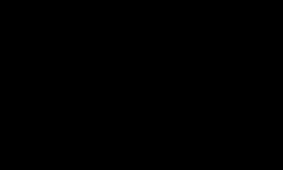
\includegraphics[width=85mm]{./imgs/im1.jpg}
\caption{\tiny{\Formular{Folha de rosto do livro {\slsc{\index{Atget, Eugène}Atget: Photographe de Paris}} (1930)}}}

\end{figure}

\index{Atget, Eugène}Atget pode ser considerado um fotógrafo do século \versal{XIX}, inspirado pelo
espírito enciclopédico do século \versal{XVIII}, atuando no século \versal{XX}. A imagem
do velho fotógrafo andarilho nas vielas de Paris, abnegado e
incompreendido, carregando uma câmera antiquada, escravo de seu ofício,
verdadeiro ``cavaleiro andante'' da fotografia --- juntamente com os dois
retratos que \index{Abbot, Berenice}\index{Abbot, Berenice}Abbot fez do fotógrafo em 1927, pouco antes de ele morrer
--- alimentaram ainda mais o mito em torno dele.

Dependendo da abordagem, \index{Atget, Eugène}Atget pode ser considerado tanto um simples
documentarista disciplinado a serviço de seu ofício quanto um grande
artista de vanguarda, precursor da fotografia moderna. O dilema entre o
operário da imagem e o artista está no centro de seu trabalho, ou
melhor, no centro da discussão sobre seu trabalho. Sim, pois ele mesmo,
a julgar pelo pouco que se sabe, nunca se importou com essas questões.
Mas, mesmo assim, o chamado ``problema \index{Atget, Eugène}Atget'' mobilizou muitos
teóricos da fotografia ao longo do século \versal{XX} (\index{Benjamin, Walter}Walter Benjamin, \index{Walker,  Evans}Walker
Evans, \index{Szarkowski, John}John Szarkowski, \index{Krauss, Rosalind}Rosalind Krauss), sempre esbarrando na falta de
documentos e declarações do próprio fotógrafo. Por mais que se mergulhe
em seu vasto acervo, o mistério permanece.

O que queria \index{Atget, Eugène}Atget? Considerá"-lo como um fotógrafo medíocre que ``deu
sorte'' em algumas imagens (grande parte de suas fotografias são
realmente desprovidas de interesse, meros registros, às vezes mal
executadas tecnicamente) é negar a carga emotiva e expressiva que o
conjunto do trabalho suscita; por outro lado, considerá"-lo um artista
visionário é correr o risco de ser desautorizado pelo próprio \index{Atget, Eugène}Atget, que
poderia dizer que ``eram meros documentos''.\footnote{De fato, na porta
  de seu estúdio lia"-se numa placa ``documentos para artistas'', pois
  algumas de suas fotografias serviam de referência para artesãos,
  artistas, pintores, caricaturistas, ilustradores e cenógrafos.} Em
defesa dessa segunda hipótese argumenta"-se que \index{Atget, Eugène}Atget seria extremamente
modesto ou ressentido, não querendo reconhecer seu próprio
mérito.\footnote{No futebol, seria como um cruzamento errado que
  resultou, involuntariamente, num golaço. Se o jogador diz que o gol
  não foi sua intenção, diminui a beleza do lance?}

Em todo caso, na América, o trabalho de \index{Atget, Eugène}Atget acabou servindo para gerar
uma importante discussão acerca da própria natureza da fotografia, um
invento humano sempre colocado entre a vocação documental e utilitária,
por um lado; e o potencial criativo e estético, por outro. \index{Atget, Eugène}Atget é
responsável, mesmo involuntariamente, pela problematização da própria
ideia de \emph{autor} e \emph{autoria} na fotografia, podendo ser
considerado o elo perdido entre a fotografia cientifista do século \versal{XIX} e
a fotografia criativa do século \versal{XX}. Hoje, tanto a obra de \index{Atget, Eugène}Atget quanto a
história de sua recepção crítica, são cruciais para entender a
fotografia moderna. Conta"-se que tão logo o \versal{MOMA} (seguramente a fim de
valorizar o próprio acervo) tenha começado a promover sua obra, os
bibliotecários dos arquivos históricos da França passaram a
reclassificar as fotografias de \index{Atget, Eugène}Atget --- que se encontravam catalogadas
por assunto --- agora por ordem de autor.

Afora as especulações, há essa carta, onde se lê: ``Esta enorme coleção,
artística e documental, está hoje concluída. Posso dizer que possuo toda
a velha Paris''. Diante dessas duas frases incrivelmente assertivas
podemos inferir que, para \index{Atget, Eugène}Atget, não há grande diferença entre a obra
artística e documental; que a própria noção de autor, como entendemos,
não existia na época; que ele conseguiu realizar inteiramente o trabalho
hercúleo a que se propôs; que o ato de fotografar exaustivamente um
lugar (ou ter em mãos essas fotografias) equivale a ``apropriar"-se''
desse lugar; que \index{Atget, Eugène}Atget circunscreveu sua obra no espaço (Paris) e no
tempo (a ``velha''); e que, dentro desse escopo, \emph{nada} escapou ao
seu olhar. Não é pouco.

Por ``velha Paris'', entende"-se a cidade que não foi atingida pela
grande reforma urbanística promovida por \index{Napoleão \versal{III}}Napoleão \versal{III} e executada pelo
\index{Haussmann, Georges-Eugène}Barão Haussmann em meados do século \versal{XIX}, que derrubou bairros inteiros e
abriu os grande eixos e bulevares, dando a Paris a monumentalidade que
vemos hoje. A Paris de \index{Atget, Eugène}Atget ainda é a cidade de malha urbana medieval,
de ruas tortuosas, escuras e úmidas, mesmo em suas últimas fotografias
dos anos 1920.\footnote{O trabalho de \index{Atget, Eugène}Atget é frequentemente confundido
  com o de \index{Marville, Charles}Charles Marville (1813-1879), fotógrafo oficial da cidade, que
  retratou Paris antes (e também depois) da grande reforma --- portanto
  cinquenta anos antes de \index{Atget, Eugène}Atget. Mesmo assim, em alguns casos, para
  diferenciar um do outro é preciso recorrer à data de realização da
  fotografia.} Mas é também a cidade afetiva, que ainda guarda uma
escala humana e pedestre. Em suas fotografias, mal aparecem os grandes
monumentos como a Torre Eiffel ou o Arco do Triunfo --- ele simplesmente
\emph{ignora} a cidade \index{Haussmann, Georges-Eugène}haussmanniana. \index{Atget, Eugène}Atget fotografa com devoção, mas
também com urgência; quer conservar em imagem a ``sua'' cidade que
restou, agora ameaçada pela construção do metrô.\footnote{Antes de
  \index{Atget, Eugène}Atget, na então desimportante cidade de São Paulo, o fotógrafo \index{Azevedo, Militão Augusto de}Militão
  Augusto de Azevedo também realizou um registro bastante sistemático
  das ruas e das construções. Mas, se em Paris o olhar de \index{Atget, Eugène}Atget estava
  voltado para o passado, aqui \index{Azevedo, Militão Augusto de}Militão parece olhar para o futuro, dando
  a São Paulo uma importância que não tinha, como se pudesse antever o
  crescimento alucinante da cidade no século \scalebox{.8}{XX}. Seu {\slsc{Álbum
    comparativo da cidade de São Paulo (1862-1887)}} é um levantamento
  metódico e pioneiro da cidade, realizado por um fotógrafo que pode ser
  chamado de visionário.} No verso de algumas fotografias, escreve:
``vai desaparecer''.

\index{Atget, Eugène}Atget parece, no entanto, utilizar"-se desse anacronismo a seu favor.
Este olhar para a cidade que guarda as marcas do passado tem
evidentemente algo de nostálgico, mas não apenas. \index{Atget, Eugène}Atget, ao trazer esta
cidade em vias de desaparecimento para o seu presente, realiza uma
operação de deslocamento temporal que acaba jogando luz sobre a cidade
em que vive, violentamente transformada por interesses do Estado. Essa
inadequação é o que faz de \index{Atget, Eugène}Atget um fotógrafo de seu tempo,
exemplificando com perfeição as observações do filósofo italiano \index{Agamben, Giorgio}Giorgio
Agamben (2009, p.~58) acerca da contemporaneidade: ``pertence
verdadeiramente ao seu tempo, é verdadeiramente contemporâneo, aquele
que não coincide perfeitamente com este, nem está adequado às suas
pretensões e é, portanto, nesse sentido, inatual; mas, exatamente por
isso, exatamente através desse deslocamento e desse anacronismo, ele é
capaz, mais do que os outros, de perceber e apreender o seu tempo''.

A fisionomia de uma cidade é resultado das transformações da história,
algo que se pode perceber desde os ínfimos detalhes (\index{Atget, Eugène}Atget fotografou
muitas aldravas, portas e escadas) até o próprio traçado das ruas.
Podemos entender a cidade como um livro decodificado à espera de ser
lido, mas isso só será possível a quem saiba decifrar seus enigmas. Para
isso, dispomos de alguns instrumentos valiosos como a câmera
fotográfica, os pés e a curiosidade. \index{Atget, Eugène}Atget faz uso exemplar desses três
instrumentos e vai se inserir numa linhagem de
andarilhos"-pesquisadores"-artistas de Paris, inaugurada por \index{Baudelaire, Charles}Baudelaire e
perpetuada pelos situacionistas nos anos 1960. Uma série de personagens
que fizeram do caminhar uma arte e da cidade um laboratório de
criatividade.

Essa autonomia da forma física da cidade, cujos enigmas estão impressos
nas paredes, no asfalto e nos próprios espaços vazios talvez explique
porquê na grande maioria das fotografias de \index{Atget, Eugène}Atget não há ninguém. Apesar
da calma aparente, a cidade vazia de \index{Atget, Eugène}Atget se revela mais como um
cenário onde algo acabou de acontecer ou está prestes a acontecer.
Assim, indiretamente, a fotografia de \index{Atget, Eugène}Atget acaba dizendo muito sobre os
cidadãos que habitam aquele espaço, sem recorrer à presença deles no
quadro fotográfico. Cria"-se uma situação de suspensão e tensão, que
levou \index{Benjamin, Walter}Benjamin (1985, p.~174) a enxergar nas fotos de \index{Atget, Eugène}Atget o cenário de
um crime, como se o espaço pudesse reter os ``indícios'' de algo que
aconteceu há pouco. Essa proposta de leitura do espaço urbano só tem a
perder com a presença de pessoas que, quando são um elemento importante
da fotografia, acabam por monopolizar a narrativa, reivindicando para si
o olhar que deveria percorrer livremente o espaço.

Mas há ainda, na carta, outros aspectos importantes. \index{Atget, Eugène}Atget diz que
``recolheu'' ou ``reuniu'' (``j'ai recueilli'') as fotografias pelas
ruas. Recolher, no entanto, não é produzir --- é juntar algo que já
existe, é ir à busca de coisas que estão disponíveis a quem tenha a a
paciência de procurar e sabedoria de achar. Além disso, chama o conjunto
de ``coleção'', que pode ser entendido tanto como a ``coleta'' dos
diversos objetos da rua capturados pela câmera quanto o próprio conjunto
material de fotografias (que quer vender). Em todo caso, coleção não é
propriamente uma obra --- colecionar é dar sentido de conjunto a coisas
esparsas, é potencializar o valor individual de uma coisa na medida em
que é comparada às outras.

\begin{figure}[!ht]

\centering
 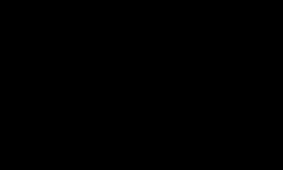
\includegraphics[width=85mm]{./imgs/im1.jpg}
\caption{\tiny{\Formular{\index{Atget, Eugène}Eugène Atget. {\slsc{Coin Rue de Seine}} (c. 1924)}}}

\end{figure}

Em \emph{A escrita da história} (1975), \index{Certeau, Michel de}Michel de Certeau oferece uma
reflexão sobre a importância do ato de colecionar. Para ele, as coleções
e os arquivos são condição essenciais para a elaboração da história. O
primeiro gesto dessa elaboração consiste em separar e reunir,
transformando os objetos em ``documentos''. Colecionar trata"-se,
portanto, de ``produzir'' documentos, recopiando, transcrevendo ou
fotografando esses objetos, deslocando"-os de seu contexto original, tal
como faz \index{Atget, Eugène}Atget. É uma ``operação técnica'' que constitui os dados:

\begin{quote}
Colecionar, durante muito tempo, é fabricar objetos: copiar ou imprimir,
reunir, classificar\ldots{} E com os produtos que multiplica, o colecionador
se toma um ator na cadeia de uma \emph{história por fazer} (ou por
refazer), de acordo com novas pertinências intelectuais e sociais. Desta
maneira, a coleção, produzindo uma transformação dos instrumentos de
trabalho, redistribui as coisas, redefine unidades de saber, instaura um
lugar de recomeço, construindo uma ``máquina gigantesca'' (Pierre
Chaunu) a qual tornará possível uma outra história (\versal{CERTEAU}, 2002,
p.~82).
\end{quote}

Por um lado, colecionar é um procedimento científico e tipológico; por
outro, uma atividade lúdica e prazerosa, como sabe qualquer criança que
já colecionou objetos. Na infância, aliás, aprendemos que há coleções
permanentemente abertas (como moedas, selos e tampinhas de garrafa) e
aquelas que se completam, proporcionando um prazer especial (álbum de
figurinhas, revistas antigas, discos de uma banda que não existe mais).
Nesse sentido, podemos dizer que \index{Atget, Eugène}Atget completou seu álbum de figurinhas
(``possuo toda a velha Paris'') e agora quer vender ao Estado.

Mas colecionar e possuir significa ainda algo mais. Qualquer coleção
reflete muito do caráter do colecionador. \index{Benjamin, Walter}Walter Benjamin (1987, p.~235), no texto \emph{Desempacotando minha biblioteca}, afirma que para o
colecionador a ideia de posse é ``a mais íntima relação que se pode ter
com as coisas: não que elas estejam vivas dentro dele; é ele que vive
dentro delas''. No mesmo sentido, para \index{Baudrillard, Jean}Baudrillard (2008, p.~98), uma
vez que se possui um objeto, podemos ``personalizá"-lo'' através de
ordenações, classificações e distribuições: ``o objeto é assim, no seu
sentido estrito, realmente um espelho: as imagens que devolve podem
apenas se suceder sem se contradizer. É um espelho perfeito já que não
emite imagens reais, mas aquelas desejadas''.

De forma análoga, a câmera fotográfica, como
percebe o cineasta \index{Wenders, Wim}Wim Wenders (2001, p.~7), tem a capacidade de fazer dois
disparos simultaneamente, um para frente e outro para trás, realizando
uma fotografia e revelando a ``atitude'' (\emph{Einstellung}) do
fotógrafo ao mesmo tempo. Para frente a câmera vê um objeto, para trás
revela um desejo. Essas observações ilustram claramente aquilo que
qualquer observador atento da obra de \index{Atget, Eugène}Atget percebe: é possível
vislumbrar o sujeito --- seja o autor, o artista, o fotógrafo, enfim, o
ser humano --- por detrás dessas imagens. A tal ponto que se torna quase
impossível distinguir a cidade retratada por \index{Atget, Eugène}Atget da personalidade do
próprio \index{Atget, Eugène}Atget.

É tentador procurar entender seu trabalho numa chave warburgiana. A
``coleção'' de \index{Atget, Eugène}Atget, da mesma forma que o \emph{Atlas Mnemosine}
(1927-1929), de \index{Warburg, Aby}Aby Warburg, é o que \index{Didi-Huberman, Georges}Didi"-Huberman (2010a, p.~45) chama
de ``aparato concreto de um pensamento'' --- algo que, no conjunto,
contém um discurso feito de imagens. Quando analisamos esse discurso,
somos obrigados a nos deparar com uma cidade mediada por uma experiência
bastante pessoal e afetiva, legitimando o uso da expressão ``Paris de
\index{Atget, Eugène}Atget'', uma cidade criada pelo fotógrafo, e que só ele seria capaz de
conceber. Com isso, entramos novamente no terreno pantanoso da mais
antiga discussão acerca da fotografia: é documento ou arte? Até onde vai
a objetividade e começa a subjetividade?

\index{Atget, Eugène}Atget realizou inúmeras belíssimas fotografias. \emph{Rue de la
Montagne"-Sainte"-Geneviève} (1924), por exemplo, é uma obra"-prima de
composição, de atmosfera, de ``sense of place''. A imagem coloca o
observador \emph{dentro} da cidade, no preciso momento em que é
surpreendido pela vista do Panteão, que surge fantasmagórico entre duas
esquinas. É uma perspectiva feita de dentro para fora da cidade,
marcando com clareza o lugar do fotógrafo, no interior da cidade
acolhedora, cujas portas, calçamento e escadas remetem à escala humana.
Ele olha com distanciamento e desconfiança para a cidade espetacular,
monumental e luminosa, que se entrevê ao longe. Entre o sujeito e o
monumento, coloca"-se uma frágil luminária, meio torta, marcando a
passagem abrupta entre os dois mundos. Do lado de cá, a cidade de \index{Atget, Eugène}Atget,
a ``velha Paris'' em processo de desaparecimento; do lado de lá, a Paris
dos grandes espaços, que se anuncia como ``cidade"-luz''.

\begin{figure}[!ht]

\centering
 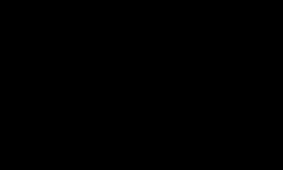
\includegraphics[width=85mm]{./imgs/im1.jpg}
\caption{\tiny{\Formular{\index{Atget, Eugène}Eugène Atget. {\slsc{Rue de la Montagne Sainte"-Geneviève}} (1924)}}}

\end{figure}

O que essa fotografia tem de beleza, uma outra, \emph{Versailles:
Escalier de l'Orangerie} (1901) tem de enigmático. Por que fotografar a
tanta distância? O que significa essa escada que leva a lugar nenhum,
terminando de repente? Na composição, 40\% da imagem é chão e 30\% é
céu. O resto é uma massa escura de folhagem, a escada distorcida (que é
grande, mas parece pequena) e uma grade que delimita o espaço de um lado
só. Cinco elementos que compõem uma imagem ``minimalista'' e
desequilibrada, que não cumpre dignamente uma função ``documental''.
Será o produto de uma displicência, ou de falta de habilidade? Ou será
que tudo isso é intencional, com o intuito de criar justamente uma
imagem misteriosa, evocativa, como num sonho? Será que o aparente vazio
esconde vestígios da presença humana? Não será essa escada que leva ao
nada uma metáfora perfeita e onírica do \emph{memento mori} a que todos
estamos submetidos?

\begin{figure}[!ht]

\centering
 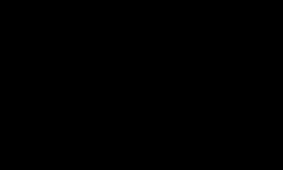
\includegraphics[width=85mm]{./imgs/im1.jpg}
\caption{\tiny{\Formular{\index{Atget, Eugène}Eugène Atget. {\slsc{Versailles: Escalier de l'Orangerie}} (1901)}}}

\end{figure}

Além desses valores estéticos encontrados em várias de suas fotografias,
é preciso reconhecer que a outra face da grandeza de seu trabalho está
no conjunto, na imensa capacidade de trabalho e na quantidade de
fotografias que produziu --- uma verdadeira ``tentativa de esgotamento de
um lugar parisiense'' (parafraseando o título do livro de \index{Perec, Georges}Georges
Perec).\footnote{Em {\slsc{Tentativa de esgotamento de um lugar
  parisiense}} (1974), \index{Perec, Georges}Georges Perec senta"-se ora num café, ora num
  banco da praça Saint"-Sulpice, em Paris, e passa a anotar
  freneticamente {\slsc{tudo}} o que se passa à sua frente durante três
  dias.} Essa atitude totalizante e enciclopédica, um levantamento
fotográfico, que percorre ``toda'' Paris escrutinando seus bairros, é o
que nos permite enxergar na obra de \index{Atget, Eugène}Atget um mapeamento poético da
cidade, sobretudo na série ``Topografia da velha Paris''.\footnote{\index{Atget, Eugène}Atget
  classificou suas fotografias em cinco temas principais:
  ``Paisagens"-documentos'' (fotografias de referência da cidade para
  serem usadas por diversos artistas), ``Arredores'' (que inclui muitas
  fotografias de Versailles), ``Paris pitoresca'' (pequenos ofícios,
  passantes, prostitutas, vitrines, interiores, veículos, entre outras
  atividades), ``A arte na velha Paris'' (sobretudo ornamentos e
  elementos decorativos) e ``Topografia da velha Paris'' (a série em que
  percorre, sistematicamente, bairro por bairro, as ruas da cidade).}
\index{Atget, Eugène}Atget é como um cartógrafo ou, mais precisamente, como o aventureiro que
precede o cartógrafo e vai a campo ``recolher'' informações que,
reunidas, formam um mapa, mesmo que seja o mapa subjetivo, afetivo, que
existe apenas em sua cabeça.

\index{Atget, Eugène}Atget não se interessou em fotografar a cidade vista de cima, embora
pudesse subir nas diversas torres da cidade, como tantos fotógrafos
fizeram. Seu trabalho tem permanentemente uma escala humana, mostrando a
cidade que se vê do nível da rua, acessível a qualquer um, reforçando
sua condição de andarilho. Em seu trabalho, a cidade não se deixa ver
numa única fotografia. A ``totalidade'' se dá pelo conjunto, pelo
acúmulo, pela coleção que se constrói no tempo e se guarda na memória. A
``Paris de \index{Atget, Eugène}Atget'' não se mostra instantaneamente; é preciso, ao
contrário, paciência e disposição para percorrer as fotografias, como
também é preciso para percorrer a cidade.\footnote{Nesse sentido, o
  trabalho de \index{Atget, Eugène}Atget é oposto ao de \index{Ferrez, Marc}Marc Ferrez. Embora contemporâneos,
  diferem em quase tudo, com exceção do interesse pela representação da
  cidade. \index{Ferrez, Marc}Ferrez é o fotógrafo do Estado, buscando uma imagem
  ``oficial'' da cidade. Está a todo momento tentando captar a beleza
  espetacular e natural do Rio de Janeiro, visto de cima, enquanto \index{Atget, Eugène}Atget
  mergulha nas entranhas de Paris. Além disso, enquanto \index{Ferrez, Marc}Ferrez realizava
  primorosas fotografias panorâmicas, impecáveis, as fotografias de
  \index{Atget, Eugène}Atget nunca primaram por esmero técnico.} Essa atitude de \index{Atget, Eugène}Atget é
essencialmente ``fotográfica''. Diferentemente de muitos de seus
contemporâneos, afasta"-se de qualquer pictorialismo, extraindo da
fotografia aquilo que ela tem de original e único, conquistando
definitivamente um território em que a pintura não pode competir. E
talvez seja esse o principal elemento que faz de \index{Atget, Eugène}Atget um precursor da
fotografia moderna, mesmo que à sua revelia.

\index{Atget, Eugène}Atget não deixou muito material para sabermos o que se passava em sua
cabeça, mas deixou, por outro lado, uma quantidade imensa de coisas que
passaram diante de seus olhos. Essas coisas são responsáveis, ao mesmo
tempo, por um \emph{imaginaire} (imaginário) e por uma \emph{imagerie}
(iconografia) da cidade de Paris. No primeiro caso, uma cidade quase
fictícia, a ``Paris de \index{Atget, Eugène}Atget'', que nenhum outro fotógrafo poderia
criar; no segundo, um documento de valor inestimável, fonte de pesquisa
que preservou para a posteridade ``toda a velha Paris''. Aqui,
poderíamos, mais uma vez, buscar a distinção entre o documentarista e o
artista, mas me parece desnecessário. O problema de \index{Atget, Eugène}Atget é o próprio
problema da fotografia, e talvez seja melhor enfrentarmos a ideia de que
não se trata de uma coisa \emph{ou} outra, mas de uma coisa \emph{e}
outra, como ele sugere na carta. \index{Atget, Eugène}Atget introduz ao mesmo tempo em que
\emph{supera} essa questão. Pode"-se discutir durante décadas (e há quem
faça) se \index{Atget, Eugène}Atget era um trabalhador disciplinado ou um gênio
incompreendido, mas uma dúvida não se pode ter: \index{Atget, Eugène}Atget era fotógrafo.

Afora a elegância com que oferece ao Estado um dos maiores legados da
história da fotografia, algo mais se depreende de sua carta. Sua
``iniciativa individual'' é aquela de quem tem um compromisso consigo,
com a cidade que lhe serve de inspiração e com o meio que lhe serve de
ferramenta --- três elementos indissociáveis em seu trabalho. Por isso,
\index{Atget, Eugène}Atget é um modelo de fotógrafo admirado pelos fotógrafos, que enxergam
em seu legado uma dedicação legítima, orientada não pelas regras de
mercado, nem por vaidade ou prestígio, mas por algo que podemos chamar
de paixão.

\chapter{Objetos}

O impulso catalográfico também orientou o trabalho do casal alemão Bernd
e Hilla \index{Becher, Bernd e Hilla}Becher que, por mais de 50 anos, se dedicou a fotografar
estruturas industriais, sobretudo na região do vale do Ruhr, na
Alemanha. Com rigor e disciplina fora do comum, os \index{Becher, Bernd e Hilla}Bechers criaram um
vastíssimo acervo fotográfico que documenta uma época em transformação
ao mesmo tempo em que provocaram importantes discussões a respeito da
linguagem fotográfica. Suas atividades como fotógrafos e também como
professores ligados à renomada Academia de Belas Artes de Düsseldorf
colocam os \index{Becher, Bernd e Hilla}Bechers entre os mais influentes fotógrafos da
história.\footnote{A Academia de Belas Artes de Düsseldorf é uma
  tradicional instituição de ensino fundada em 1762, inicialmente famosa
  pelas pinturas de paisagens de tendência romântica e naturalista. A
  partir dos anos 1930 foi enquadrada nos princípios estéticos do
  nazismo e foi parcialmente destruída ao final da Segunda Guerra
  Mundial. Depois da Guerra a instituição renasce e passa a ser uma
  importante referência na arte contemporânea da Alemanha Ocidental.
  Nesse período, \index{Beuys, Joseph}Joseph Beuys e \index{Richter, Gerhard}Gerhard Richter foram alunos e também
  professores da instituição. O ensino de fotografia teve início em
  1976, com Bernd \index{Becher, Bernd e Hilla}Becher.}

O casal se dedicou a um registro sistemático da arquitetura industrial
da Europa, que passava por uma profunda transformação social e econômica
após a Segunda Guerra Mundial. Lançaram seu olhar para caixas d'água,
armazéns, altos"-fornos, torres de extração, silos, torres de
refrigeração, depósitos de cascalho, usinas de tratamento, tanques de
gás, fornos de cal, casas em enxaimel e parques industriais inteiros.
Muitas dessas estruturas, símbolos de um pujante passado industrial,
estavam condenadas ao desaparecimento. Havia, portanto, um sentido de
urgência que moveu os \index{Becher, Bernd e Hilla}Bechers a preservar essa memória através da
fotografia. Nesse contexto, a fotografia já plenamente desenvolvida como
técnica se colocava como o instrumento ideal, oferecendo uma exatidão,
precisão e rapidez que a pintura e o desenho não poderiam oferecer.

Essa ``arqueologia industrial'' precisa ser entendida no contexto de um
país traumatizado pela derrota e pela devastação da guerra. A Alemanha
tinha, em meados do século \versal{XX}, uma dificuldade enorme em lidar com seu
passado recente. Depois de tanta barbárie, era muito difícil remexer nas
feridas ainda abertas, restando apenas o caminho de um \emph{mea culpa}
profundo ou de uma abordagem ``objetiva'', que pretendesse retratar a
realidade sem julgamento. Os \index{Becher, Bernd e Hilla}Bechers, optando por este segundo caminho
--- com sua técnica ``neutra'' e atemporal, onde não se vê nenhuma pessoa
retratada --- foram em busca, como muitos artistas alemães"-ocidentais do
pós"-guerra, de uma ``desistorização'' desse passado recente.

As estruturas fotografadas pelos \index{Becher, Bernd e Hilla}Bechers também simbolizam o passado
alemão digno de ser lembrado, pois representam a grande contribuição
tecnológica, científica e industrial que a Alemanha deu ao mundo. Diante
da vergonha causada pela guerra, foi preciso voltar os olhos para as
qualidades que esse mesmo país possui. É preciso lembrar também que,
para essa geração, a memória dos anos entreguerras da República de
Weimar (1919-1933) ainda estava viva quando o país experimentou um
período democrático e de liberdades individuais, apesar dos problemas
econômicos (que, ao final, levaram à ascensão do nazismo). Esse é
justamente o período da infância de Bernd \index{Becher, Bernd e Hilla}Becher, que cresceu junto às
indústrias de Siegen, onde podia ``ver, ouvir e sentir o cheiro da
siderúrgica'' (\versal{ZIEGLER}, 2011, p.~161).

Há, portanto, a meu ver, por detrás de toda a neutralidade pretendida
pelos \index{Becher, Bernd e Hilla}Bechers, uma alta carga de afetividade que move os fotógrafos, em
busca de registrar não apenas as estruturas que vão desaparecer, mas
também de ir ao encontro das próprias memórias que sofreram um golpe
violentíssimo nos anos imediatamente anteriores. Dessa forma, o trabalho
do casal pode ser visto tanto como um registro desapaixonado de
estruturas industriais desprovidas de beleza quanto uma obra melancólica
e pessoal num país simbolicamente devastado em busca de sua própria
identidade.

\begin{figure}[!ht]

\centering
 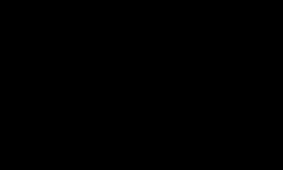
\includegraphics[width=85mm]{./imgs/im1.jpg}
\caption{\tiny{\Formular{\index{Becher, Bernd e Hilla}Bernd e Hilla Becher. {\slsc{Depósitos de cascalho}} (1988-2001)}}}

\end{figure}

Se há um termo associado aos \index{Becher, Bernd e Hilla}Bechers, e disparador dos mais apaixonados
e raivosos discursos sobre a natureza da fotografia, esse termo é
\emph{objetividade}. Desde a indignação de \index{Baudelaire, Charles}Baudelaire no século \versal{XIX} até
os dias de hoje, este é um tema que perpassa a história crítica da
fotografia. Problema sem solução, uma vez que se confunde com a própria
natureza do meio. Sem querer entrar mais profundamente nesse terreno
pantanoso, cabem algumas considerações a respeito do conceito de
objetividade no trabalho dos \index{Becher, Bernd e Hilla}Bechers.\footnote{Compartilho da opinião de
  \index{Didi-Huberman, Georges}Didi"-Huberman (2004, p.~59, trad.~minha) sobre a objetividade fotográfica: ``em geral pede"-se
  muito ou muito pouco às imagens. Se pedimos muito a elas --- isto é,
  `toda a verdade' --- sofreremos uma decepção: as imagens não são nada
  mais do que fragmentos arrancados, restos de filmes. Ou talvez pedimos
  muito pouco às imagens: ao relegá"-las logo de cara à esfera do
  simulacro, as excluímos do campo histórico como tal. Ao relegá"-las à
  esfera do documental, apartamos as imagens de sua fenomenologia, de
  sua especificidade, de sua própria substância''.}

Há claramente nessas fotografias o desejo de alcançar o maior grau de
precisão e informação possível, uma tentativa de substituição da
percepção seletiva do olho humano pelo registro mecânico da câmera. Os
\index{Becher, Bernd e Hilla}Bechers partem da premissa de que os objetos fotografados têm a
capacidade de ``expressarem a si mesmos'', não cabendo ao fotógrafo
acrescentar nenhuma outra camada de opinião ou de subjetividade, cabendo
a ele apenas a abertura da câmera para que a realidade imprima a si
mesma diretamente sobre a película, como um \emph{decalque}. Quanto mais
deixar os objetos ``falarem por si'', melhor --- pois eles são capazes de
contar a própria história, sem necessidade de interpretação. Num
documentário de 2002, Hilla \index{Becher, Bernd e Hilla}Becher deixa isso bem claro:

\begin{quote}
Para mim, o propósito da fotografia é ver de uma maneira objetiva. Por
que eu deveria tentar projetar meus próprios sentimentos ou meu estado
de espírito em algo que já se expressa por si só? É claro que a
objetividade é o oposto da subjetividade, temos problemas para separar
os dois, um começa onde o outro termina. E a objetividade não significa
que a verdade tenha sido encontrada, longe disso, significa que o objeto
representado pode falar por si (\versal{BERND}, 2002).
\end{quote}

Há um termo em inglês que tenta dar conta dessa abordagem. O verbo ``to
deadpan'' significa receber impressões externas sem demonstrar resposta
emocional. Através do ``deadpanning'', eventos são (supostamente)
reduzidos à sua factualidade, enquanto qualquer arroubo ``criativo'' é
largamente reprimido. É um termo que representa uma posição artística
altamente artificial, mas que, com frequência, é associado ao trabalho
dos \index{Becher, Bernd e Hilla}Bechers e de outros tantos fotógrafos associados à busca dessa
``neutralidade'' estética.

No entanto, a meu ver, não se trata tanto da busca de uma objetividade
utópica, onde a verdade se revela e nada se esconde. Trata"-se mais de um
processo de ``dessubjetivação'', de tentativa de eliminação do sujeito
até onde for possível. A fotografia ``deadpan'' deve ser entendida não
tanto como uma visão documental ou ``objetiva'' do mundo, mas como uma
retórica de objetividade, como uma forma de problematizar o tema da
verdade na representação artística, utilizando, para isso, a fotografia
como instrumento privilegiado.

Esse processo se revela claramente na técnica empregada pelo casal.
Entendo a fotografia dos \index{Becher, Bernd e Hilla}Bechers como uma técnica de eliminação de tudo
o que pode ser eliminado no processo fotográfico. Eles eliminam a cor
(usando filmes preto e branco), o grão fotográfico (usando grande
formato), a distorção (corrigindo a perspectiva e usando teleobjetivas),
as sombras (fotografando em dias nublados, o que elimina também os
desenhos de nuvens no céu), a folhagem (fotografando no outono e no
inverno), as pessoas (esperando o momento adequado), o contexto
(isolando os objetos), a autoria (fazendo uso de uma técnica rígida e
reprodutível), a surpresa (elegendo um único assunto), a individualidade
dos objetos (agrupando"-os, como veremos), a passagem do tempo (usando da
mesma técnica por toda a vida --- nesse sentido é admirável a dificuldade
em se distinguir as primeiras das últimas fotos). O que resta é a
estrutura fotografada da forma mais crua e neutra possível. Se se
tratasse de um retrato, seria a fotografia preto e branco de uma pessoa
nua, de frente, em pé, imóvel, sem expressão, num fundo branco. Há,
portanto, apesar da aparente objetividade, uma série de decisões
importantes tomadas pelos fotógrafos como, de resto, em todo tipo de
fotografia.

Os \index{Becher, Bernd e Hilla}Bechers parecem colocar a fotografia a serviço da ``visão correta'', \label{grid}
como se seguissem as recomendações do educador \index{Comenius}Comenius que, na
\emph{Grande didática}, de 1641, ensinava a maneira adequada de ver um
objeto:

\begin{quote}
Falaremos agora do modo pelo qual os objetos devem apresentar"-se aos
sentidos, se a impressão tiver de ser bem definida. Isso poderá ser
facilmente compreendido se considerarmos os processos da visão real.
Para que o objeto seja visto claramente, é necessário: (1) que seja
posto diante dos olhos; (2) não muito longe deles, mas a uma distância
razoável; (3) não de lado, mas bem defronte dos olhos; (4) de modo que a
frente do objeto não esteja desviada, mas dirigida para o observador;
(5) que os olhos primeiro apreendam o objeto como um todo; (6) e depois
passem a distinguir as partes; (7) inspecionando"-as do começo ao fim;
(8) que a atenção se fixe em cada uma e todas as partes; (9) até que
todas sejam apreendidas por meio de seus atributos essenciais. Se esses
requisitos forem adequadamente observados, a visão ocorre com êxito, mas
esse êxito será apenas parcial caso um deles seja negligenciado
(\index{Comenius}\versal{COMENIUS} apud \versal{ALPERS}, 1999, p.~201).
\end{quote}

Do ponto de vista metodológico, os \index{Becher, Bernd e Hilla}Bechers fazem parte de uma tradição
catalográfica iluminista, iniciada no século \versal{XVIII}, que procurou
sistematizar e popularizar todo o conhecimento disponível. Nessa época
surgem as enciclopédias e os dicionários, impulsionados pelo
desenvolvimento das técnicas de impressão. Além disso, uma série de
expedições científicas e exploratórias são enviadas ao redor do mundo,
sobretudo aos países ``exóticos'', a fim de coletar todo tipo de
material para uma Europa ávida de conhecimento.\footnote{Uma das mais
  importantes obras, fruto desse espírito, é a {\slsc{Descrição do
    Egito}}, publicada entre 1809 e 1822, na França. Trata"-se uma
  gigantesca obra gráfica realizada a mando de \index{Bonaparte, Napoleão}Napoleão Bonaparte que
  mobilizou centenas de artistas, matemáticos, engenheiros, arquitetos,
  gravadores e impressores, tanto na pesquisa do material durante a
  expedição, quanto no imenso trabalho de confecção dos livros. Com mais
  de 3000 desenhos, a obra pretendia ser a compilação mais completa
  possível dos aspectos da arquitetura, fauna, botânica, mineralogia e
  dos tipos humanos do Egito.}

Podemos traçar a origem desse impulso classificatório nas ciências
naturais, mais precisamente na botânica ou na zoologia, em que as
plantas do mesmo gênero ou animais da mesma espécie são agrupados a fim
de serem comparados. Para os \index{Becher, Bernd e Hilla}Bechers, assim como para esses cientistas,
fotografar significa recolher, descrever, classificar, catalogar,
comparar, colecionar e arquivar as coisas.\footnote{Ver também o
  {\slsc{Atlas}} (iniciado em 1962), de \index{Richter, Gerhard}Gerhard Richter.} O catálogo é um
instrumento científico --- portanto uma forma de conhecimento --- no qual
percebemos as semelhanças pelas diferenças, e as diferenças pelas
semelhanças. A ideia por trás é que uma série de objetos deve adquirir
mais sentido do que a soma dos elementos individuais, assim como uma
história é mais do que uma soma de palavras.

\begin{figure}[!ht]

\centering
 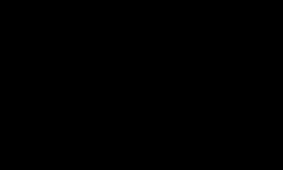
\includegraphics[width=85mm]{./imgs/im1.jpg}
\caption{\tiny{\Formular{{\slsc{Descrição do Egito}}. Capitéis e colunadas da ilha de Philae}}}

\end{figure}


Há claramente algo de enciclopédico na atitude de quem busca reunir todo
o conhecimento sobre um determinado assunto.\footnote{A descrição total
  está também presente no conto {\slsc{A biblioteca de Babel}} (1941), de
  \index{Borges, Jorge Luis}Jorge Luis Borges. O escritor argentino descreve uma imensa
  biblioteca, com seus salões e escadarias, que possui todos os livros
  de 410 páginas possíveis de serem escritos, cada um com uma combinação
  diferente das letras do alfabeto, resultando numa biblioteca
  inapreensível, embora finita (\scalebox{.8}{BORGES}, 2007, p.~558).} Assim como há
algo de mapeamento em toda atitude enciclopédica. Na fotografia, essa
abordagem se desenvolveu na Alemanha a partir dos anos 1920 com os
fotógrafos da chamada \emph{Nova Objetividade} como \index{Sander, August}August Sander, \index{Blossfeldt, Karl}Karl
Blossfeldt e \index{Renger-Patzsch, Albert}Albert Renger"-Patzsch; e tem como grande modelo a
monumental e inacabada obra de \index{Sander, August}Sander \emph{Pessoas do século \versal{XX}}
(1911-1945). \index{Sander, August}Sander deixou milhares de retratos, registrando pessoas e
grupos das mais diversas camadas sociais, idades, profissões e origens
numa tentativa de produzir uma documentação exaustiva e completa da
fisionomia da República de Weimar --- uma obra manifestadamente admirada
pelo casal.

Essa abordagem sistemática levou os \index{Becher, Bernd e Hilla}Bechers a desenvolverem suas famosas
``tipologias'' --- uma forma de apresentação das fotografias em
\emph{grids} de 9, 12 ou 15 imagens, normalmente do mesmo tipo de
estrutura industrial.\footnote{Os {\slsc{grids}} dos \index{Becher, Bernd e Hilla}Bechers se assemelham a um quadrado mágico. Essa tabela matemática (que remonta há séculos) consiste numa disposição de números num {\slsc{grid}} regular, onde a soma de cada fileira vertical, horizontal e diagonal é a mesma.} Com as tipologias, foi possível reconhecer nas
estruturas industriais uma rica morfologia que passara desapercebida até
então, evidenciando diferenças arquitetônicas conforme a região, o uso,
os materiais disponíveis e a necessidade. E, porque não dizer, acabaram
revelando também uma espécie de \emph{beleza} oculta nos edifícios
puramente funcionais.

Além dos grupos de estruturas semelhantes, construíram também algumas
séries em que mostram o mesmo edifício visto por diversos pontos de
vista --- as chamadas \emph{Abwicklungen}. Em \emph{Sternbuschweg 362}
(1972), o mesmo prédio é mostrado por oito vistas diferentes, que
correspondem às quatro fachadas e às quatro diagonais do prédio, como se
o fotógrafo captasse o objeto a partir dos quatro pontos cardeais e dos
quatro pontos colaterais. Ao mesmo tempo em que mostra simultaneamente
``todos'' os ângulos do edifício (como no cubismo), há a sensação de
rotação, como se o objeto estivesse colocado sobre uma superfície
giratória que pudéssemos manipular, sugerindo uma dimensão temporal e
cinematográfica. Há claramente uma estratégia de mapeamento do edifício,
uma tentativa de recuperar suas três dimensões, fazendo uso da
bidimensionalidade fotográfica, e prefigurando as ferramentas 3D das
plataformas digitais.

\begin{figure}[!ht]

\centering
 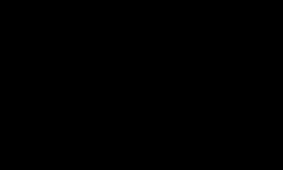
\includegraphics[width=85mm]{./imgs/im1.jpg}
\caption{\tiny{\Formular{\index{Becher, Bernd e Hilla}Bernd e Hilla Becher. {\slsc{Sternbuschweg 362}}, Alemanha (1972)}}}

\end{figure}

Como se vê, há claramente uma transformação das estruturas fotografadas
em \emph{objetos}. A neutralidade visual, o isolamento das estruturas
arquitetônicas de seu contexto, a tridimensionalidade e a classificação
segundo sua morfologia contribuem para essa percepção que, mais tarde,
vai colocar o trabalho dos \index{Becher, Bernd e Hilla}Bechers próximo ao campo da
escultura.\footnote{Não por acaso, o livro mais importante do casal
  chama"-se {\slsc{Esculturas anônimas}} (1970) e, em 1990, receberam o
  {\slsc{Leão de Ouro}} na Bienal de Veneza justamente na categoria de
  escultura.} A serialidade, repetição e diferenciação, por sua vez,
aproximaram os \index{Becher, Bernd e Hilla}Bechers dos artistas minimalistas norte"-americanos,
sobretudo de \index{Andre, Carl}Carl Andre (1972, p.~59), para quem essas fotografias ``registram a
existência transitória de estruturas puramente funcionais e revelam o
grau em que a forma é determinada pelos requisitos invariáveis da
função''.

Essa revalorização das estruturas industrias deve muito a \index{Le Corbusier}Le Corbusier
que, num famoso artigo de 1920, publicou fotos de silos e depósitos de
grãos americanos, enaltecendo a beleza da forma decorrente da função.
Além da base de uma arquitetura funcionalista, essa valorização da
arquitetura industrial traz também uma crítica à própria noção de autor.
Para os \index{Becher, Bernd e Hilla}Bechers, o anonimato do design industrial merece ser levado a
sério tanto quanto qualquer obra autoral.

Os \index{Becher, Bernd e Hilla}Bechers direcionaram a atenção para algo que não tinha importância
anteriormente, ou que nunca havia sido visto daquela maneira. Essa é uma
ideia que evoca a famosa frase de \index{Klee, Paul}Paul Klee (2001, 9. 73): ``a arte não
reproduz o visível, mas faz o visível''. Com isso, os \index{Becher, Bernd e Hilla}Bechers tornaram
visível um legado que poderia ter sido apagado da história, não fossem
essas fotografias. Mais do que isso, \emph{criam} (para usar uma palavra
cara ao mundo artístico) esses objetos e um modo de vê"-los até então
inédito. A questão, portanto, já não é se a fotografia reproduz a
realidade, mas, ao contrário, se a realidade corresponde ao que essas
fotografias nos mostram. Nessa inversão, a realidade passa então a ser
valorizada e examinada segundo o grau de semelhança com a
fotografia.\footnote{Corroboro aqui considerações de \index{Zweite, Armin}Armin Zweite. Ver
  \scalebox{.8}{BECHER}, Bernd; \scalebox{.8}{BECHER}, Hilla. {\slsc{Tipologías}}. Madri: La Fabrica, 2010.}
Nesse sentido, o trabalho dos \index{Becher, Bernd e Hilla}Bechers parece evocar o pensamento lapidar
de \index{Winogrand, Garry}Garry Winogrand: ``eu fotografo para descobrir como as coisas ficam
quando são fotografadas'' (\versal{LONGWELL}, 1972, p.~4).

Ao mesmo tempo em que provocaram os limites da fotografia documental, os
\index{Becher, Bernd e Hilla}Bechers penetraram no meio das artes, abrindo o caminho que seria
seguido por diversos fotógrafos na segunda metade do século \versal{XX}. Fizeram
uso da capacidade plena da fotografia, já prevista e temida por
\index{Baudelaire, Charles}Baudelaire no polêmico artigo de 1859 em que compara a
fotografia com as artes ditas mais ``nobres'':

\begin{quote}
Que ela enriqueça rapidamente o álbum do viajante e devolva a seus olhos
a precisão que faltava à sua memória, que ela ornamente a biblioteca do
naturalista, amplie os animais microscópicos, ou mesmo, que ela
acrescente ensinamentos às hipóteses do astrônomo, que ela seja enfim a
secretária e o guarda"-notas de quem quer que precise, em sua profissão,
de uma absoluta precisão material, até aí, nada melhor. Que ela salve do
esquecimento as ruínas decadentes, os livros, as estampas e os
manuscritos que o tempo devora, as coisas preciosas cuja forma irá
desaparecer e que pedem um lugar no arquivo de nossa memória, ela terá
nossa gratidão e será ovacionada. Mas se lhe for permitido usurpar o
domínio do impalpável e do imaginário, de tudo aquilo que apenas tem
valor porque o homem lhe acrescenta alma, então, que desgraça a nossa!
(2007, p.~13).
\end{quote}

Os \index{Becher, Bernd e Hilla}Bechers fotografam seus ``objetos'' com compaixão, como se
entendessem o sofrimento interno dessas estruturas ``feias'' e
desprezadas. Com suas fotografias, que cumprem a função documental e
criativa ao mesmo tempo, justificam o temor de \index{Baudelaire, Charles}Baudelaire. Criaram uma
obra ao mesmo tempo objetiva e pessoal, restritiva e enciclopédica,
extremamente expressiva, mesmo escondida por detrás de um véu de
aparente inexpressividade. Seu trabalho se insere num espaço cultural
que não sabíamos que pudesse existir. Situa"-se numa intersecção
improvável onde a fotografia, a escultura, a indústria, as ciências
naturais, a arquitetura, a arte conceitual e, sobretudo, a história, se
encontram.

\chapter{\emph{Elefante} (2003), de Gus Van Sant}

No filme \emph{Elefante} (2003), o cineasta norte"-americano \index{Sant, Gus Van}Gus Van Sant
faz do mapeamento um elemento narrativo essencial.\footnote{O filme foi
  vencedor da {\slsc{Palma de Ouro}} do Festival de Cannes, em 2003, além
  do prêmio de melhor diretor.} O enredo é basicamente uma recriação do
dramático ``massacre de Columbine'', ocorrido em 20 de abril de 1999,
quando dois adolescentes fortemente armados promoveram um tiroteio na
Columbine High School --- uma escola de ensino médio americana ---,
matando treze pessoas, antes de cometerem suicídio. A complexa ação
durou quase uma hora e foi meticulosamente planejada com antecedência
por esses dois alunos. O filme é uma ficção baseada no intenso
noticiário da época, e não pretende ser um documentário. Todo o filme se
desenrola no próprio dia do massacre, desde a normalidade das primeiras
horas do dia, até o tiroteio final.

\begin{figure}[!ht]

\centering
 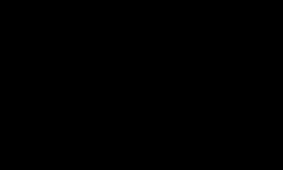
\includegraphics[width=85mm]{./imgs/im1.jpg}
\caption{\tiny{\Formular{\index{Sant, Gus Van}Gus Van Sant. {\slsc{Elefante}} (2003)}}}

\end{figure}

O filme faz uso de um sofisticado jogo de câmeras para envolver o
espectador. \index{Sant, Gus Van}Van Sant filma os personagens e seus deslocamentos adotando
seus próprios pontos de vista.\footnote{Como no conto {\slsc{A
  construção}}, de \index{Kafka, Franz}Kafka. Ver página~\pageref{construcao}.} Para isso, faz uso
de longos planos"-sequência, com a câmera seguindo e filmando os
personagens de costas, acompanhando seus deslocamentos pelo espaço. O
plano"-sequência é uma tomada em movimento contínuo --- um engenhoso
recurso cinematográfico que coloca a narrativa do filme em ``tempo
real'', produzindo a sensação de veracidade, uma vez que reproduz a
passagem do tempo como de fato experimentamos na vida, ou seja, sem
corte.\footnote{{\slsc{Festim diabólico}} ({\slsc{Rope}}, 1948), de \index{Hitchcock, Alfred}Alfred
  Hitchcock, representa uma tentativa de se criar um filme com apenas um
  longo plano"-sequência (embora haja alguns cortes). É um
  thriller psicológico que se passa inteiramente dentro de um
  apartamento. Dois planos"-sequência virtuosos se encontram em {\slsc{Soy
    Cuba}} (1948), uma produção cubano"-soviética, dirigida por \index{Kalatozov, Mikhail}Mikhail
  Kalatozov. Outro exemplo é {\slsc{Arca russa}} (2002), de \index{Sokurov, Aleksandr}Aleksandr
  Sokurov, rodado inteiramente no Museu Hermitage, de São Petersburgo,
  numa única tomada de 87 minutos.} Dos 88 planos do filme, 9 são
planos"-sequência, filmados com uma s\emph{teadicam}, técnica que
estabiliza as imagens e contribui para a naturalidade da filmagem,
criando uma sensação de fluidez parecida com nosso olhar.

A história é apresentada pela primeira vez através do olhar de John
(praticamente o personagem principal) e depois é repetida através do
olhar de outros personagens cujos trajetos se cruzam. Com o acúmulo das
tomadas, o filme coloca o espectador num lugar de onisciência, sabendo
mais que os personagens. Dessa forma, o espectador vai construindo a
narrativa pouco a pouco e consegue, em vários momentos, antecipar a
ação. Segundo o próprio diretor (\versal{BAECQUE}, 2003, trad.~minha), ``a ideia
era começar com os dados do noticiário, ou seja, a localização de cada
um deles durante o tiroteio, e seus movimentos de acordo com as
atividades do dia, e depois filmar os percursos, que vão se cruzando''.

Como os personagens se deslocam constantemente e repetidamente pelos
corredores da escola, o espectador vai se familiarizando com esse espaço
--- vai, literalmente, \emph{mapeando} gradativamente a escola,
exatamente com o rato no labirinto de \index{Tolman, Edward}Tolman. Há, portanto, uma
espacialização da ação que vai se constituir como um elemento
fundamental para a narrativa do filme. Com o espaço mapeado, e a
sensação de algo sinistro, o filme ganha uma enorme tensão, que só vai
ser liberada no final, de forma provavelmente trágica. O espectador
passa a conhecer o espaço da escola e sabe onde está o perigo, mas o
personagem não sabe. Em alguns momentos do filme, ocorre alertar o
personagem e temos vontade de dizer: ``não abra essa porta!''.

\index{Sant, Gus Van}Gus Van Sant confessa sua paixão pelos mapas (coleciona mapas de
desertos) e pelos esquemas infográficos dos jornais: ``minha primeira
lembrança é o mapa do assassinato de \index{Kennedy, John Fitzgerald}Kennedy: o trajeto do carro, como
foi posicionado o corpo do presidente, a localização do atirador, o
caminho da bala. Me lembro perfeitamente de todos esses detalhes através
dos mapas que os jornais publicaram'' (\versal{BAECQUE}, 2003, trad.~minha).

\begin{figure}[!ht]

\centering
 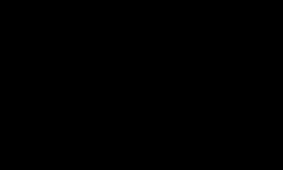
\includegraphics[width=85mm]{./imgs/im1.jpg}
\caption{\tiny{\Formular{\index{Sant, Gus Van}Gus Van Sant. Mapa de {\slsc{Elefante}} (2003)}}}

\end{figure}


Numa entrevista ao jornal francês \emph{Libération}, o diretor desenhou
de cabeça o mapa da escola onde rodou as cenas, mostrando a importância
do espaço cartográfico na própria construção do filme.\footnote{O mesmo
  mapa aparece num dos menus do \scalebox{.8}{DVD} do filme. É possível escolher a
  sequência que se quer ver escolhendo, no mapa, o percurso do
  personagem.} Nesse mapa, anotou os lugares principais: a academia, a
biblioteca, o campo de futebol, a cafeteria, o laboratório fotográfico e
a entrada principal, organizados ao redor do corredor central, local dos
principais encontros dos personagens e que serve como uma ``espinha
dorsal'' do espaço. Anota também, em cores diferentes, o trajeto de cada
um dos personagens. O \versal{X} indica o lugar onde iniciaram o trajeto e onde
foram baleados. O próprio diretor explica, nessa mesma entrevista, a
importância desse esquema e de como, ele mesmo, acabou mapeando
cognitivamente o espaço: ``é algo que eu repeti tantas vezes, na minha
cabeça e depois num mapa bastante parecido com este, antes de realizá"-lo
de verdade com os rapazes e com a câmera, que eu realmente conheço de
memória cada detalhe desse lugar e cada variação desses deslocamentos''
(\versal{BAECQUE}, 2003, trad.~minha).

O filme claramente se inspira no universo dos videogames,
sobretudo nos chamados \emph{first"-person shooter} (\versal{FPS}), um subgênero
dos jogos de tiro, que simula o ponto de vista subjetivo do atirador,
como se o quadro e o campo de visão fossem a mesma coisa. E, portanto,
como se o jogador e o personagem do jogo fossem a mesma pessoa. Nesses
jogos, a tela mostra o cenário que se pode percorrer e, na parte
inferior, vê"-se a arma que está sendo utilizada. São, em geral, bastante
violentos (os inimigos morrem à frente, em circunstâncias escabrosas) e
muitos deles se passam em ambientes labirínticos, com muitas portas e
corredores, como a escola retratada no filme. Nesses jogos, a ameaça é
iminente, e a vida do jogador (portanto, do atirador) também depende de
um correto mapeamento cognitivo do espaço. De fato, os atiradores do
filme aparecem no filme jogando \emph{Doom} (1993), o videogame que ---
juntamente com \emph{Wolfenstein 3D} (1992) --- popularizou
definitivamente os jogos \versal{FPS}.

\begin{figure}[!ht]

\centering
 \includegraphics[width=85mm]{./imgs/im1.jpg}
\caption{\tiny{\Formular{\index{Sant, Gus Van}Gus Van Sant. {\slsc{Elefante}} (2003)}}}

\end{figure}


O uso do videogame no contexto do filme sugere a influência
desses jogos em ações violentas e reforça o perigo da indistinção entre
o mundo real e o mundo fictício na sociedade contemporânea.
\emph{Elefante} é, no fundo, um filme político que, sem adotar uma
postura mais ideológica (como no filme de \index{Moore, Michael}Michael Moore, sobre o mesmo
assunto), alerta para o perigo do consumo, da alienação, da publicidade,
da futilidade e para toda sorte de males da sociedade atual, sobretudo
nos Estados Unidos. E, no contexto que aqui nos interessa, mostra que o
mapeamento é, de fato, uma capacidade humana poderosa, mas que também
pode ser usada para os fins mais sinistros.

\chapter{\emph{Spin out, for Robert Smithson} (1973), de Richard Serra}

Para alcançar a obra \emph{Spin out, for \index{Smithson, Robert}Robert Smithson} (1973), de
\index{Serra, Richard}Richard Serra, é preciso deixar para trás os gramados bem cortados do
jardim de esculturas do museu Kröller"-Müller, e entrar por uma trilha
que atravessa uma área mais selvagem do parque, como um bosque. A
paisagem logo se modifica e dá lugar a uma mata mais densa e mais
escura. A umidade aumenta e a temperatura cai um pouco.

A trilha atravessa um pequeno desfiladeiro que vai se afunilando e, mais
adiante, se abre numa clareira elíptica, como um pequeno fundo de vale
rodeado pela mata. A trilha atravessa todo esse espaço pelo nível do
chão, longitudinalmente, como se houvesse uma entrada e uma saída do
outro lado. Lembra, pelo tamanho e pelo formato ovalado, um pequeno
anfiteatro romano.

\begin{figure}[!ht]

\centering
 \includegraphics[width=85mm]{./imgs/im1.jpg}
\caption{\tiny{\Formular{\index{Serra, Richard}Richard Serra. {\slsc{Spin out, for \index{Smithson, Robert}Robert Smithson}} (1973).\break Museu Kröller"-Müller, Holanda (\index{Vieira, Tuca}foto: Tuca Vieira)}}}

\end{figure}

A obra se encontra nessa clareira. É formada por três chapas de aço
\emph{corten} de medidas iguais, com três metros de altura, doze de
comprimento e trinta e quatro centímetros de espessura, enfiadas na
própria encosta. Isso é o que lhes dá sustentação ao mesmo tempo em que
esconde uma parte da chapa. Quem chega pela trilha, vindo do museu, vê
duas chapas do lado esquerdo e uma do lado direito. Vistas desse ponto,
nenhuma delas têm realmente um formato regular e não parecem ter as
mesmas dimensões. Cada uma se apresenta de uma forma distinta, com
tamanho aparente distinto, a uma distância distinta, iluminada de
maneira distinta, com cores e luminosidade levemente distintas. À
primeira vista, elas são tudo menos iguais.

As três lâminas, aparentemente saídas da própria colina, convocam o
espectador para dentro. É incontornável o impulso de se dirigir ao
centro desse espaço, rodeado pela encosta e pelas peças. Em todo caso,
nesse ponto, não haveria alternativa. Ou seguimos a trilha e vamos para
o centro do vale ou retornamos. Não há como contornar, nem como buscar
outro acesso ao conjunto.

Uma vez ``dentro'' desse espaço, o visitante se encontra inevitavelmente
sujeito a uma estranha força rotativa que o obriga a girar, a fim de
apreender o entorno. Com isso, toma consciência do formato elíptico do
vale e percebe, agora, cada uma das chapas individualmente, buscando
diferenças e semelhanças entre elas, embora seja difícil colocar duas no
mesmo campo de visão. A visão de uma leva à outra, que leva à outra, que
leva à outra, provocando uma rotação do corpo no sentido anti"-horário,
uma experiência que logo toma um carácter cinematográfico e
entorpecente, onde o giro e a repetição das formas provocam uma espécie
de tontura. É quando se percebe o movimento que a obra propõe e quando
se justifica o próprio título --- \emph{Spin out} ---, expressão de
difícil tradução, mas que sugere algo que \emph{gira para fora}, um
rodopio sem controle, um vórtice, uma centrífuga.

\begin{figure}[!ht]

\centering
 \includegraphics[width=85mm]{./imgs/im1.jpg}
\caption{\tiny{\Formular{\index{Serra, Richard}Richard Serra. {\slsc{Spin out, for \index{Smithson, Robert}Robert Smithson}} (1973).\break Museu Kröller"-Müller, Holanda (foto: \index{Vieira, Tuca}Tuca Vieira)}}}

\end{figure}

Aqui se intui que as chapas sejam da mesma dimensão, ao mesmo tempo em
que se constata que isso não importa, uma vez que não se pode comprovar.
Na verdade, a suspeita de elas serem iguais é mais interessante do que a
certeza. Para o observador, à medida que o tempo passa, as diferenças
entre elas se tornam aparentes e, aos poucos, cada uma delas vai
adquirindo uma ``personalidade'' própria. Uma está na ``entrada'' e
outra na ``saída'' do percurso, como recebendo e se despedindo do
observador, e criam uma relação entre si. A outra está um pouco mais
afastada da trilha, na parte mais aberta da elipse onde, justamente por
isso, a grama e o mato podem crescer sem serem pisoteados pelos
visitantes.

Estamos sem dúvida no centro do vale, mas isso não significa que estamos
exatamente no centro da obra. Agora a experiência cinética dá lugar à
tentativa de apreensão geométrica e visual do espaço, em busca de uma
ordem oculta que possa revelar algum segredo e, consequentemente, a
verdadeira intenção do artista. É tentador prolongar visualmente as
chapas, como se elas brotassem da encosta e se projetassem para o lado
oposto, assim como é tentador desenhar mentalmente o triângulo
imaginário formado pelas extremidades de cada uma delas. A rigor, é
possível criar uma série de triangulações imaginárias entre as chapas, e
calcular a posição dos diversos ``centros'' no interior desses
triângulos.

\index{Serra, Richard}Serra (1994, p.~16, trad.~minha) diz que as placas foram distribuídas
como os ponteiros de um relógio, marcando 12, 4 e 8 horas
aproximadamente, formando um triângulo isósceles, de quarenta e seis
metros (o lado maior) e vinte e quatro metros (os lados menores).
Suponho que os vértices desse triângulo sejam as extremidades escondidas
das chapas, enterradas na encosta. Faz sentido, mas, como ele mesmo
afirma, isso não importa.

Esse exercício abstrato, numa tentativa de compreender a obra em planta,
procurando pontos convergentes e formas geométricas ocultas logo se
mostra inútil e mesmo estúpido. A liberdade de experimentar a obra
desprovido de um mapa e a inexistência de ``significados'' na forma
geométrica abstrata dão prazer especial à experiência. Não é preciso nem
desejável ``sair'' da obra e buscar um ponto de vista externo,
imaginando a vista que se tem do alto. Não é preciso desenhar
mentalmente um mapa, nem polígonos e retas imaginárias: ``o foco da arte
para mim é a experiência de vivenciar através das peças, e essa
experiência pode ter muito pouco a ver com aspectos físicos da obra de
arte'' (1994, p.~16, trad.~minha), sugere o artista justamente a
respeito de \emph{Spin out}. Aqui, a dimensão temporal, narrativa e
cumulativa se sobrepõe ao próprio objeto. \index{Serra, Richard}Serra está mais preocupado com
a experiência e com o percurso do que com a imagem (ele próprio afirma
isso categoricamente), mais preocupado com o corpo do que com os olhos,
mais preocupado com a dimensão fenomenológica do que com os aspectos
visuais da obra. Mais preocupado, enfim, com o mapeamento do que com o
mapa.

Portanto, reconsiderando, o exercício geométrico, na verdade, não é
totalmente inútil. Ele é útil na medida em que revela com mais clareza
sua própria inutilidade, como algo que se deve experimentar para poder
descartar. Uma vez feito isso, podemos relaxar e desfrutar da obra de
forma mais experiencial e fluida, buscando não mais as relações entre as
partes, mas entre todo o conjunto e nosso próprio corpo e, se quisermos
ir mais adiante, entre tudo isso e as supostas forças cósmicas na
natureza --- como se estivéssemos num desses monumentos megalíticos (como
Stonehenge), onde se buscam alinhamentos solares, relações com eclipses,
estrelas e pontos cardeais. Provavelmente nada se encontrará diretamente
nesse sentido, mas é inegável o fluxo de forças e vetores sugerido pela
obra, e a situação de ``santuário'' que o local sugere --- uma espécie
de templo que, se não traz exatamente a paz espiritual, convida à
reflexão e ao silêncio.

Assim que nos livramos da força giratória do redemoinho imaginário
central, é possível perambular pela clareira e explorar seu ambiente em
mais detalhe. Para isso, é preciso abandonar o percurso sugerido pela
trilha e caminhar à deriva pelos espaços mais ou menos delimitados pelas
placas. São espaços que funcionam mais como subdivisões propostas, mais
como campos, do que como compartimentos. E, assim como uma chapa pede
para ser comparada à outra, esses espaços também se relacionam entre si
e adquirem, cada um deles, sua própria ``personalidade'' provocando no
espectador sensações distintas.

\begin{figure}[!ht]

\centering
 \includegraphics[width=85mm]{./imgs/im1.jpg}
\caption{\tiny{\Formular{\index{Serra, Richard}Richard Serra. Detalhe de {\slsc{Spin out, for \index{Smithson, Robert}Robert Smithson}} (1973). Museu Kröller"-Müller, Holanda}}}

\end{figure}

A princípio, a precisão do corte, a ortogonalidade racional das peças e
a coloração entram em contraste frontal com as formas orgânicas da
natureza e o verde da grama e das folhas. Mas há uma relação mais
complexa em jogo. Ao mesmo tempo em que a natureza é \emph{alterada}
pela presença das peças, estas também têm seu sentido \emph{alterado}
pelo simples fato de estarem nesse local (basta imaginarmos as chapas
numa siderúrgica, descontextualizadas). E uma visão mais aproximada
mostra que, não apenas o sentido é alterado, como também o próprio
objeto. Um olhar mais atento e o próprio toque dos dedos nas peças
revelam diversos detalhes da superfície como a textura e a corrosão
misturadas ao musgo. As peças reagem à ação da natureza (chuva, frio,
calor, umidade) e se transformam com o tempo, num processo de corrosão
irreversível que, no limite, vai destruir a obra.

É interessante imaginar como deve ser esse lugar nas outras estações do
ano, respondendo às transformações sazonais: no outono, com as folhas no
chão fazendo ruído ao serem pisadas, a mata menos verde, mais marrom; no
inverno sem folhagem, com o anfiteatro natural se mostrando por inteiro
(um folheto mostra o local coberto de neve, desprovido de cores e
reduzido a três elementos: as placas, as árvores e o branco).

\begin{figure}[!ht]

\centering
 \includegraphics[width=85mm]{./imgs/im1.jpg}
\caption{\tiny{\Formular{Folheto da obra {\slsc{Spin out, for \index{Smithson, Robert}Robert Smithson}} (1973).\break Museu Kröller"-Müller, Holanda}}}

\end{figure}

Isso nos faz imediatamente pensar que a obra não se resume aos três
elementos de aço. Dela fazem parte também os espaços segmentados, a
clareira, as encostas, a ferrugem, o mato, a trilha, os vetores
imaginários, a luz, as estações do ano, o tempo, o percurso, nós, enfim,
tudo aquilo que é modificado pela presença das três chapas. Não há
começo nem fim, não há fronteiras além daquela imposta pela própria
clareira. \index{Serra, Richard}Serra acredita no potencial da escultura em ``criar seu
próprio lugar e espaço'' (1994, p.~171, trad.~minha). Esta situação
ilustra com precisão a frase do artista \index{Heizer, Michael}Michael Heizer a respeito da
Land Art, movimento artístico surgido na década de 1960, bastante
influente sobre o trabalho de \index{Serra, Richard}Serra: ``o trabalho não é \emph{posto} em
um lugar, ele \emph{é} esse lugar'' (\versal{COTRIM}; \versal{FERREIRA}, 2006, p.~275,
grifo nosso).

Seguindo a trilha e saindo da clareira, a curiosidade nos impele a olhar
para trás. A visão que se tem é bastante parecida com a imagem da
chegada. Por um momento pode"-se pensar que é a mesma imagem, agora
invertida ou espelhada. Fica ainda mais claro como as chapas mudam de
posição conforme o deslocamento do corpo. A imobilidade das peças (que,
sem dúvida, têm um peso considerável) é apenas ilusória, bastando um
passo para fazer todo o conjunto se mover.\footnote{Essa concepção do
  espaço baseada no tempo e no movimento na obra de \index{Serra, Richard}Serra é algo que o
  artista atribui à descoberta dos jardins zen de Kyoto, no Japão
  (\scalebox{.8}{SERRA}, 2014, p.~244).} Com isso, há uma fusão de espaço e movimento,
colocando em xeque nossa concepção de espaço tradicional, com um único
ponto de vista central, herdeiro da perspectiva renascentista.

\begin{figure}[!ht]

\centering
 \includegraphics[width=85mm]{./imgs/im1.jpg}
\caption{\tiny{\Formular{\index{Serra, Richard}Richard Serra. {\slsc{Spin out, for \index{Smithson, Robert}Robert Smithson}} (1973).\break Museu Kröller"-Müller, Holanda (foto: \index{Vieira, Tuca}Tuca Vieira)}}}

\end{figure}

Esse movimento visual é exatamente aquilo que chamamos de paralaxe, ou
seja, o deslocamento aparente de um objeto conforme se muda o ponto de
observação. Esse efeito dialético faz o observador perceber a
importância de sua própria posição relativa, adquirindo, portanto,
``conscientização da fisicalidade do tempo, do espaço e do movimento''
(\versal{SERRA}, 2014, p.~25). Esta preocupação foi explicitada pelo próprio
artista (2014, p.~25) ao comentar \emph{Shift} (1970) --- uma obra
realizada pouco antes, mas que guarda muitas semelhanças com \emph{Spin
Out}: ``eu queria uma dialética entre a percepção que se tem do lugar em sua totalidade e a relação que se estabelece com o campo ao percorrê"-lo''. O resultado seria um modo do indivíduo medir a si próprio diante da indeterminação do terreno, um processo que ele mesmo chama de ``pensar com os pés'' (``thinking on your feet''). \index{Serra, Richard}Serra propõe, portanto, uma conscientização espacial que anda de mãos dadas com a experiência crítica, numa linha próxima ao ``efeito de distanciamento'' do teatro épico de Brecht.\footnote{Ver página~\pageref{brecht}.} Bem diferente, portanto, de uma simples contemplação passiva.

Podemos estender essa proposta estética para bem além do mundo
artístico.\footnote{O fotógrafo alemão \index{Tillmans, Wolfgang}Wolfgang Tillmans (2012, pp.~16-47), durante uma
  palestra na Royal Academy of Arts de Londres em 2012, faz uma bela
  reflexão sobre as potencialidades da paralaxe como forma de
  conhecimento: ``Quando tinha dez ou onze anos, eu sabia que quando
  tivesse trinta e seis aconteceria um trânsito de Vênus, um fenômeno
  astronômico extremamente raro que acontece uma vez a cada 128 anos,
  depois uma vez mais em 8 anos, e depois novamente em 128 anos. O que
  acontece é que Vênus, a Terra e o Sol ficam perfeitamente alinhados ---
  tal como acontece no eclipse total do Sol, onde a Lua a Terra e o Sol
  ficam perfeitamente alinhados. Então vemos o pequeno disco de Vênus
  movendo"-se durante 6 horas em frente ao disco do Sol. Este
  acontecimento foi particularmente importante para a história da
  ciência, tendo levado à descoberta da Nova Zelândia e da Austrália
  pelo Capitão Cook que partiu em missão para medir o tempo de entrada e
  de saída de Vênus no disco do Sol, e comparar com a mesma medição
  feita em Londres, e com essas medições poderia determinar a paralaxe
  e, consequentemente, a distância entre a Terra e o Sol. Esta era, na
  época, a única maneira de nos localizarmos no universo, de saber onde
  estamos em relação ao que nos rodeia. Para mim, assistir este evento
  foi uma experiência extremamente comovente, como se os mecanismos do
  sistema solar estivessem bem diante de nossos olhos''.} Não
seria a postura ``paraláctica'' uma proposta de leitura crítica que pode
nos ajudar a ajustar a distância entre o sujeito e a alteridade,
desvendando, pelo menos em parte, as complexidades do mundo
contemporâneo? A consciência das distâncias, dos diversos pontos de
vista e das mutações do espaço visual relativo, que a paralaxe coloca em
evidência, não seria justamente aquilo que nos falta para escaparmos do
espaço imersivo desse mundo saturado de imagens, sem distanciamento
crítico e uniformizado? Não seria a obra paraláctica, que ``procura
enquadrar o enquadrador enquanto este enquadra o outro'', como define
\index{Foster, Hal}Hal Foster (2014, p.~185), um equivalente artístico à proposta de
mapeamento cognitivo pregada por Fredric \index{Jameson, Fredric}Jameson?

Como se pode notar, é bastante difícil fotografar uma obra como essa.
Seguindo a trilha, e subindo a encosta, é possível encontrar um ponto no
meio do mato de onde se vê o conjunto, de cima para baixo. De fato, é
uma fotografia descritiva e atraente, que mostra bem o campo de força
triangular no centro da clareira, mas não dá conta da \emph{experiência}
da obra. Olhar de cima para baixo é olhar de fora, excluindo o próprio
corpo que --- uma vez que é parte da obra --- não pode ser excluído. É
novamente buscar o mapa do espaço, uma visão gestáltica que quase anula
seu verdadeiro entendimento.

\begin{figure}[!ht]

\centering
 \includegraphics[width=85mm]{./imgs/im1.jpg}
\caption{\tiny{\Formular{\index{Serra, Richard}Richard Serra. {\slsc{Spin out, for \index{Smithson, Robert}Robert Smithson}} (1973).\break Museu Kröller"-Müller, Holanda (foto: \index{Vieira, Tuca}Tuca Vieira)}}}

\end{figure}

\emph{Spin out}, portanto, não é exatamente uma obra que se vê, mas uma
obra que se percorre, ou melhor, que se \emph{atravessa}. E na ideia de
travessia está, como vimos, a possibilidade de surpresa, de aventura, de
narrativa, de descoberta e, sobretudo, de experiência. Este é o
exercício pré"-cartográfico necessário, que foi substituído pelos mapas,
atrofiando nossa capacidade de leitura do espaço. Da experiência de
atravessar esse lugar, não resta apenas uma imagem ou uma fotografia,
mas sobretudo uma coleção de sensações complexas guardadas na memória. E
a memória, embora esteja diretamente relacionada à nossa própria
sobrevivência, é uma capacidade humana em desuso, cada vez mais delegada
aos aparelhos e às imagens mecânicas.

\chapter{Fotografar para ver}

\index{Serra, Richard}Serra dedica \emph{Spin out} ao amigo \index{Smithson, Robert}Robert Smithson, que havia morrido
pouco antes num acidente aéreo. A arte contemporânea tende a classificar
o trabalho de \index{Serra, Richard}Serra como pós"-minimalista, enquanto a obra de \index{Smithson, Robert}Smithson é
associada, de uma forma geral, à Land Art. São dois movimentos
norte"-americanos, surgidos mais ou menos na mesma época, que
compartilham o desejo de desafiar as convenções da escultura moderna
(\index{Serra, Richard}Serra chegou a ajudar \index{Smithson, Robert}Smithson a realizar alguns trabalhos). No
entanto, apresentam uma série de diferenças significativas, uma delas
diz respeito ao uso da fotografia. Para \index{Serra, Richard}Serra (2014, p.~81) a fotografia
nega a experiência temporal da obra, pois fotografar é reduzir a
escultura ao plano chato da fotografia com o intuito de torná"-la própria
ao consumo. Para ele, não se pode experimentar a escultura fora do local
onde ela está.

No que diz respeito ao uso da fotografia, a Land Art se coloca
diametralmente oposta a \index{Serra, Richard}Serra. Na Land Art, muitas vezes o registro
fotográfico era um meio incontornável para acessar a obra ou era mesmo
parte integrante dela. Há dois fatores que contribuem para esse uso
intenso da fotografia. Em primeiro lugar porque essas obras, muitas
vezes, se situam em lugares remotos e de difícil acesso. Com isso, a
fotografia passa a ser o veículo de acesso privilegiado, o transporte
virtual entre a obra e o espectador, cumprindo uma das funções mais
básicas da fotografia, desde sua invenção do século \versal{XIX}. Além disso, o
uso da fotografia permitia a percepção completa das obras de grande
dimensão, muitas vezes com forte caráter gráfico, apreensível somente
do alto. Portanto, para os artistas da Land Art, se não for
possível ir até o local da obra ou vê"-la desde um ponto de vista aéreo,
tudo bem: há fotografias.

No entanto, artistas da Land Art foram bem além do uso estritamente
utilitário da fotografia. Eles perceberam que não seria possível fazer
uso dela sem lidar com a linguagem específica do meio fotográfico.
Nesses trabalhos, a fotografia aparece não apenas como registro, mas
como um instrumento de investigação e ferramenta crítica. Os artistas da
Land Art têm consciência do aspecto artificial da fotografia --- herdeira
privilegiada das regras de perspectiva renascentista --- e vão, na
maioria das vezes, acentuar conscientemente essa artificialidade,
desconstruindo sua pretensão objetiva --- eles sabem que é preciso
desconfiar da imagem fotográfica. Não por acaso, muitos desses artistas
não se enxergam como fotógrafos (é sintomático que \index{Smithson, Robert}Robert Smithson use
uma \emph{Instamatic 400}, uma câmera popular que produz fotos de baixa
qualidade). Se perguntados, talvez digam que são ``artistas que utilizam
da fotografia como ferramenta do trabalho'', assim como um pintor usa de
pigmentos e pincéis.\footnote{Ver página~XXXX.}

A Land Art pode ser entendida como um rompimento com as regras da
paisagem pictórica. Nesses trabalhos, a natureza não é mais apenas
\emph{contemplada}, podendo o artista intervir diretamente nela. Na Land
Art, os artistas são escultores que não se contentam em modelar os
objetos e se dedicam à própria transformação física do território,
criando paisagens artificiais, como numa proposta de ``nova natureza''.
Há, portanto, um rompimento definitivo da barreira invisível que separa
o sujeito do objeto visto. É como se pudéssemos entrar dentro da
paisagem para modificá"-la, rompendo a moldura através da qual se enxerga
o mundo. Dessa forma, o artista não pode mais aceitar o ``quadro''
imposto pela fotografia --- com suas regras rígidas, como se fosse uma
janela aberta para o mundo --- e vai usá"-la de forma crítica e
distanciada, consciente da ilusão que a imagem fotográfica provoca. E
uma vez que a própria paisagem é artificializada, não há mais lugar para
o ``olhar natural''. Com isso, a fotografia passa a ser não apenas uma
testemunha, mas um modo de fabricar a obra e de construir a própria
realidade. Para o filósofo francês \index{Tiberghien, Gilles}Gilles Tiberghien (2005, p.~15), não
se trata mais de verificar como a arte se comporta diante da natureza,
mas como a natureza se comporta diante da arte.

Isso vai acontecer de diversas formas. Na série \emph{Yucatan mirror
displacements} (1969), por exemplo, \index{Smithson, Robert}Robert Smithson cria um arranjo de
espelhos na paisagem, fotografa e desmonta o arranjo --- cria, portanto,
uma obra \emph{para ser fotografada} e que vai existir apenas como
fotografia. \index{Heizer, Michael}Michael Heizer fotografa suas ``esculturas negativas'' no
deserto, em ângulo baixo, sem parâmetro de escala, fazendo as
intervenções parecerem muito maiores do que são. A famosa \emph{Spiral
jetty} (1970), de \index{Smithson, Robert}Smithson, é mais conhecida pelas imagens aéreas, que
transformam a espiral sinuosa praticamente numa abstração gráfica sobre
o fundo de coloração rara do Grande Lago Salgado de Utah. O
\emph{Lightning field} (1977) de \index{Maria, Walter De}Walter De Maria precisa ser visto no
instante preciso do cair de um raio para revelar sua potencialidade,
situação mais fácil de encontrar nas fotografias do local do que no
próprio local.

Saindo um pouco da Land Art, mas permanecendo em sua zona de influência,
há os registros fotográficos das caminhadas solitárias de \index{Long, Richard}Richard Long,
mostrando pequenas modificações no terreno --- são imagens"-resíduo de uma
performance efêmera que acabou de acabar. O \emph{Reichstag embrulhado}
(1995) de \index{Christo e Jeanne-Claude}Christo e Jeanne"-Claude, é um cartão"-postal que pede para ser
fotografado à exaustão pelos turistas. Já o \emph{Vertical earth
kilometer} (1977), do mesmo \index{Maria, Walter De}De Maria, é uma barra de latão de um
quilômetro enterrada na Friedrichsplatz, em Kassel, da qual se vê apenas
a superfície da extremidade, com poucos centímetros de diâmetro --- uma
obra que se recusa a ser vista e, portanto, se recusa a ser fotografada.

\begin{figure}[!ht]

\centering
 \includegraphics[width=85mm]{./imgs/im1.jpg}
\caption{\tiny{\Formular{\index{Smithson, Robert}Robert Smithson. {\slsc{Yucatan mirror displacements}} (1969)}}}

\end{figure}

\begin{figure}[!ht]

\centering
 \includegraphics[width=85mm]{./imgs/im1.jpg}
\caption{\tiny{\Formular{\index{Smithson, Robert}Robert Smithson. {\slsc{Spiral jetty}} (1970)}}}

\end{figure}

\begin{figure}[!ht]

\centering
 \includegraphics[width=85mm]{./imgs/im1.jpg}
\caption{\tiny{\Formular{\index{Christo e Jeanne-Claude}Christo e Jeanne"-Claude. {\slsc{Reichstag embrulhado}} (1995)}}}

\end{figure}

\begin{figure}[!ht]

\centering
 \includegraphics[width=85mm]{./imgs/im1.jpg}
\caption{\tiny{\Formular{\index{Maria, Walter De}Walter De Maria. {\slsc{Vertical earth kilometer}} (1977),\break Kassel, Alemanha (foto: \index{Vieira, Tuca}Tuca Vieira)}}}

\end{figure}

A \emph{Spiral jetty} (1970), de \index{Smithson, Robert}Smithson --- a mais emblemática obra da
Land Art --- permite duas leituras principais: pode ser experimentada
como uma escultura à maneira do trabalho de \index{Serra, Richard}Richard Serra, onde o
visitante descobre sua forma à medida que percorre o local; ou pode ser
apreendida do alto através de uma fotografia ou filmagem (supondo que
alguns terão a oportunidade de sobrevoar o local). Portanto, ou
exploramos a obra fisicamente, caminhando sobre ela, com sua
materialidade, seus jogos de luz e cor (a obra muitas vezes fica
parcialmente submersa no lago salgado), e imaginamos a forma geral; ou,
do alto, dominamos a forma geral sacrificando a experiência
fenomenológica. Essa é a mesma diferença que existe entre estar fora e
estar dentro, estar ausente e estar presente, entre ver e sentir. É a
diferença entre mapa e mapeamento. O problema é que essas duas
percepções não podem ser vividas simultaneamente, resultando no que
\index{Tiberghien, Gilles}Gilles Tiberghien (2005, p.~15) chama de ``princípio estético de
incerteza'' da Land Art.\footnote{Esse tipo de experiência dupla não é
  exclusividade da Land Art. Há uma série de obras, sobretudo no campo
  da arquitetura, que sugerem uma apreensão do alto, de onde alguma
  forma geométrica se revela. Assim são os jardins mogóis na Índia, os
  templos de Angkor, os jardins de Versalhes, os memoriais soviéticos de
  Berlim, Stonehenge, o Pentágono, Brasília. Algumas dessas obras (penso
  no Túmulo de Humaium, em Delhi e em Angkor Wat) possuem uma
  organização artificial, simétrica e geométrica de suas formas que se
  revela através da intuição espacial, gerando no espectador uma espécie
  de conforto sensorial pelo fato de estar num espaço medido e regrado,
  apreensível cognitivamente. A simetria obedece ao princípio do
  equilíbrio e da harmonia, mas também ao princípio da previsibilidade.
  Se isto está desse lado, está também do outro. Uma imagem mental que
  se comprova através do desenho, da fotografia ou do mapa.} Se por um
lado podemos enxergar nessa duplicidade uma riqueza de sentidos e uma
problematização da questão objeto/representação (como também nos
\emph{Nonsites}, de \index{Smithson, Robert}Smithson), por outro resulta numa ambiguidade no que
diz respeito à própria proposição da obra, levantando algumas questões:
o homem faz ou não faz parte da obra? Ela deve ser experimentada ou
apenas vista? Deve provocar sensações ou impõe uma leitura única?

\begin{figure}[!ht]

\centering
 \includegraphics[width=85mm]{./imgs/im1.jpg}
\caption{\tiny{\Formular{\index{Smithson, Robert}Robert Smithson. {\slsc{Nonsite}}, Oberhausen (1968)}}}

\end{figure}

\index{Serra, Richard}Richard Serra soluciona essa questão recusando radicalmente qualquer
leitura gestáltica da sua obra. Às perguntas anteriores, responde: a
obra não existe sem o sujeito, deve ser experimentada \emph{in loco},
não impõe uma leitura única. Para ele, a fotografia aérea apresenta a
obra violentamente de uma vez só, destruindo a ``multiplicidade''
visual. Mesmo que seus livros apresentem belas fotos do alto (quase
sempre as mesmas), elas são um mero registro, cumprindo o papel de
ilustração. Essas fotos, assim como os textos e as entrevistas, não
pretendem nem podem substituir a experiência. Já as obras da Land Art
são conhecidas e analisadas sobretudo através das ilustrações e dos
livros.

O ``princípio estético de incerteza'' de que fala \index{Tiberghien, Gilles}Tiberghien se torna
ainda mais radical nos \emph{Nonsites} (1968). \index{Smithson, Robert}Smithson leva para dentro
da galeria objetos coletados num determinado \emph{site}, além de mapas
e fotografias desse lugar. Com isso, o que estava fora vem para dentro
da galeria, e o que está dentro é remetido de volta para fora, como num
jogo de espelhos. Esse movimento incessante faz com que a obra não
esteja nem aqui nem ali, nem na paisagem nem em sua representação,
escapando a qualquer tipo de interpretação definitiva. É uma operação
conceitual e dialética que atinge o centro da ideia convencional de
representação associada aos mapas e às fotografias. \index{Foster, Hal}Hal Foster (2014, p.~174) atribui a essas operações cartográficas e geológicas de \index{Smithson, Robert}Smithson
uma transformação radical da ideia de \emph{localização} da arte, onde a
galeria, a instituição, o terreno natural e as próprias redes discursivas
se embaralham

Mas a contribuição mais significativa de \index{Smithson, Robert}Smithson, no que diz respeito
ao uso da fotografia, se dá quando o artista se afasta um pouco da Land
Art e se envereda para o campo mais conceitual da arte. A obra que
tensiona esses limites conceituais da fotografia é o relato \emph{A tour
of the monuments of Passaic, New Jersey} (1967). Trata"-se de uma
publicação com textos e imagens que descreve uma incursão do artista à
sua cidade natal --- um subúrbio industrial e decadente de Nova Jersey.
Nesse relato, \index{Smithson, Robert}Smithson trata a realidade como se tudo fosse imagem. Há
no texto um trecho crucial, o momento chave dessa transformação. Após
tomar o ônibus em Nova York, o autor chega à ponte que dá acesso a
Passaic:

\begin{quote}
O ônibus passou pelo primeiro monumento. Dei o sinal e desci na esquina
da Union Avenue com a River Drive. O monumento era uma ponte que
conectava o condado de Bergen com o condado de Passaic. O sol do meio"-dia dava um caráter cinematográfico ao lugar, transformando a ponte e o
rio numa foto superexposta. Fotografá"-los com minha \emph{Instamatic 400} foi
como fotografar uma fotografia. O sol tornou"-se uma monstruosa lâmpada
que projetava uma série de ``fotogramas'' nos meus olhos através de
minha \emph{Instamatic}. Quando cruzei a ponte, era como se eu caminhasse sobre
uma fotografia enorme feita de madeira e aço, e abaixo, o rio era como
um enorme filme que não mostrava mais que uma imagem em branco contínua
(\versal{SMITHSON}, 1996, p.~70, trad.~minha).
\end{quote}

\begin{figure}[!ht]

\centering
 \includegraphics[width=85mm]{./imgs/im1.jpg}
\caption{\tiny{\Formular{\index{Smithson, Robert}Robert Smithson. {\slsc{A tour of the monuments of Passaic}},\break New Jersey (1967). Publicado na revista {\slsc{Artforum}}}}}

\end{figure}

Logo que o autor desce do ônibus, uma série de transformações ocorrem. O
sol a pino ilumina excessivamente a cena, causando uma espécie de
alucinação, como miragens no deserto. A ponte se torna ``monumento''
(objeto que representa algo memorável); ela e o rio se tornam uma
fotografia (uma representação da realidade) ``superexposta'' (que
recebeu mais luz do que deveria, resultando numa imagem excessivamente
clara, que machuca os olhos); essa fotografia superexposta se torna
outra fotografia; o sol se torna uma lâmpada (uma fonte de luz
artificial); as imagens se tornam fotogramas (uma decomposição da
realidade); o rio se torna um filme (fotografias em sucessão criando
ilusão de movimento).

Ao atravessar a ponte (o primeiro ``monumento''), é como se o autor
atravessasse um portal, além do qual a relação convencional e
hierárquica entre objeto e representação não existisse mais.\footnote{A
  Passaic de \index{Smithson, Robert}Smithson pode ser entendida como uma versão adulta e
  desencantada do ``País das Maravilhas'', de \index{Carroll, Lewis}Lewis Carroll --- um mundo
  de absurdo e fantasia que também se acessa por um portal (o buraco do
  coelho): ``tantas coisas estranhas tinham acontecido recentemente que
  Alice começou a pensar que pouquíssimas coisas eram de fato
  impossíveis''. Ver \scalebox{.8}{CARROLL}, Lewis. {\slsc{Alice's Adventures in
    Wonderland}}. Londres: Vintage Books, 2012, p.~11, (trad.~minha).} Ele
rompe uma barreira invisível e \emph{entra} na fotografia (uma
reprodução precária da realidade), chegando a um universo suspenso e
onírico, onde as noções estabelecidas de espaço e tempo deixam de fazer
sentido, onde tudo se transforma em imagem, reprodução e representação,
cujo referente não existe mais.\footnote{Para \index{Wisnik, Guilherme}Guilerme Wisnik (2012b, p.~82), a
  operação conceitual de \index{Smithson, Robert}Smithson se coloca numa posição simetricamente
  oposta aos trabalhos e textos do artista neoconcreto brasileiro \index{Oiticica, Hélio}Hélio
  Oiticica. {\slsc{Tropicália}} (1969), por exemplo, é um penetrável
  (ainda não se usava o termo ``instalação'') labiríntico, repleto de
  coisas que lembram uma favela carioca, como panos, plantas, areia,
  araras, barracos improvisados e até um aparelho de televisão. O
  público caminha descalço, experimentando sensações diversas. \index{Oiticica, Hélio}Oiticica
  assim descreve a obra: ``antes de fazer estas novas cabines, eu tive a
  ideia de me `apropriar' de lugares que eu gostava, lugares reais, onde
  eu me senti vivo. De fato, o penetrável {\slsc{Tropicália}}, com sua multidão
  de imagens tropicais, é uma espécie de condensação de lugares
  reais. {\slsc{Tropicália}} é um tipo de mapa. É um mapa do Rio, e é um mapa da
  minha imaginação. É um mapa no qual você entra'' (\scalebox{.8}{OITICICA FILHO} et
  al., 2009). Portanto, diferentemente de \index{Smithson, Robert}Smithson, que ``desrealiza'' o
  espaço, \index{Oiticica, Hélio}Oiticica extrai dos lugares reais que visita uma série de
  experiências sensoriais, sensações abstratas, memórias espaciais ---
  além de todo um imaginário simbólico brasileiro --- para transformá"-las
  numa obra que convida o próprio espectador a experimentar essas
  sensações. A obra penetrável como ``mapa'' --- portanto como
  representação do espaço --- é resultado das deambulações do artista,
  tanto pelas vielas das favelas quanto pelos labirintos de sua própria
  imaginação, ou seja, é resultado de um processo de mapeamento.
  {\slsc{Tropicália}} é portanto um mapa que carrega consigo a experiência
  que lhe deu origem. A diferença para o mapa tradicional, que mostra o
  mundo pronto e acabado é que, nas instalações de \index{Oiticica, Hélio}Oiticica, o público é
  convidado a participar, traçando seu próprio percurso, obedecendo ao
  próprio tempo. É uma obra ao mesmo tempo generosa e libertária, na
  medida em que compartilha uma experiência, mas não impõe um discurso
  único.} Nesse mundo das aparências, uma ponte
desimportante, uma caixa de areia e tubulações decrépitas podem ser
monumentos. Na verdade, depois de atravessado o portal, qualquer coisa
pode ser qualquer coisa, bastando, para isso, a vontade do artista e seu
poder de \emph{designação}. O espaço geográfico, dando lugar a um espaço
de pura representação, pode ser escrito e desenhado novamente. Esse
relato --- em que imagem e texto são indissociáveis --- pode ser entendido
como uma operação \index{Duchamp, Marcel}duchampiana de deslocamento, que transforma Passaic
num lugar fantasioso onde qualquer coisa pode ser um \emph{ready"-made}.
O autor não diz que o objeto \emph{se parece} com um monumento. Ao dizer
que isso \emph{é} um monumento, isso \emph{passa a ser} um monumento por
designação do artista e, como tal, merece ser fotografado. Na Passaic de
\index{Smithson, Robert}Smithson, fotografia, mapa e território são uma coisa só.

\chapter{O corpo como lápis}

Podemos dizer, portanto, que, se para \index{Serra, Richard}Richard Serra o mapeamento é
presencial e sensorial, para \index{Smithson, Robert}Smithson trata"-se sobretudo de uma
estratégia conceitual. O artista que busca conciliar essas duas
propostas é o ``walking artist'' britânico \index{Long, Richard}Richard Long, que há mais de
quarenta anos faz do ato de andar uma proposta artística. Seu trabalho
mais conhecido, \emph{A line made by walking} (1967), registrado numa
belíssima fotografia, ajudou a redefinir o conceito de escultura e é
considerado por alguns críticos um dos pontos altos da arte do século
\versal{XX}.\footnote{A obra de \index{Long, Richard}Long seria, para a escultura, o que o
  {\slsc{Quadrado negro}} (1915), de \index{Malevich, Kazimir}Kazimir Malevich, é para a pintura: um
  ``ponto zero''. Ver \scalebox{.8}{LONG}, Richard; \scalebox{.8}{FUCHS}, Rudi. {\slsc{Richard Long.}} Londres: Thames and Hudson, 1986.} Trata"-se de uma linha reta
criada pelos passos do artista ao caminhar e pisotear na grama --- um
rastro.

Por vezes associado à Land Art, o trabalho de \index{Long, Richard}Long se opõe à
monumentalidade norte"-americana (como no \emph{Double negative}
{[}1970{]}, de \index{Heizer, Michael}Michael Heizer, por exemplo), criando formas efêmeras e
dotadas de uma poética particular e delicada. As caminhadas de \index{Long, Richard}Long às
vezes deixam \emph{marcações} na paisagem, como arranjos de pedras
formando esculturas, às vezes nem isso. Mas, diferentemente dos artistas
da Land Art, que empregavam máquinas pesadas e engenharia para a
construção das obras, o único meio empregado por \index{Long, Richard}Long é o próprio corpo.
Ele trabalha solitariamente, criando as esculturas com as próprias mãos,
como um artesão cujo atelier é o próprio mundo. Com sua simplicidade, o
resultado é bem menos espetacular que o de seus colegas norte"-americanos
mas, por outro lado, abrange conceitualmente uma área muito maior se
pensarmos que qualquer alteração da paisagem, por mais reduzida que
seja, pode modificar a paisagem como um todo.\footnote{\index{Borges, Jorge Luis}Jorge Luis Borges
  em {\slsc{Atlas}} (1984), seu livro de viagens escrito com \index{Kodama, María}María Kodama,
  assim descreve sua visita ao Egito: ``A unos trescientos o
  cuatrocientos metros de la Pirámide me incliné, tomé un puñado de
  arena, lo dejé caer silenciosamente un poco más lejos y dije en voz
  baja: {\slsc{Estoy modificando el Sahara}}'' (\scalebox{.8}{BORGES}, 2007c, p.~533).}
Mas essa intervenção não se dá como um ataque à paisagem, mas como
tentativa de diálogo entre o homem e o mundo, consciente da diferença de
escala que existe. Seus arranjos circulares de pedra, ou em outros
formatos de apelo universal, sugerem uma busca espiritual de harmonia
com a natureza, que encontra eco nos monumentos de pedra megalíticos,
como Stonehenge.

\begin{figure}[!ht]

\centering
 \includegraphics[width=85mm]{./imgs/im1.jpg}
\caption{\tiny{\Formular{\index{Long, Richard}Richard Long. {\slsc{A line made by walking}} (1967)}}}

\end{figure}

O arquiteto e professor italiano \index{Careri, Francesco}Francesco Careri (2013, p.~51), que
investiga o ato de caminhar como prática estética, sugere que quando
atravessamos um espaço novo, recebendo múltiplos estímulos, percebendo e
mapeando aos poucos o ambiente, estamos culturalmente modificando esse
espaço. Dessa forma, o ato de caminhar, mesmo não sendo uma construção
física de um espaço, é capaz de transformar os lugares e seus
significados, relacionando"-se com o universo da arquitetura. Considerado
como ato perceptivo e criativo ao mesmo tempo, leitura e escrita do
território, o caminhar \emph{produz} lugares, afirma \index{Careri, Francesco}Careri. A ideia do
caminhar como arte é, segundo o próprio \index{Long, Richard}Long (2009), ``proporcionar uma
maneira simples de explorar relações entre tempo, distância, geografia e
medida''. Com isso, \index{Long, Richard}Long se utiliza do próprio corpo para medir o mundo.

A obra em si é o ato efêmero do caminhar, quase uma performance. Essas
caminhadas são representadas em fotografias, mapas, textos e esculturas,
que depois são expostas na galeria ou nos museus. Portanto, \index{Long, Richard}Long não
abre mão nem da experiência física do espaço (tão importante para \index{Serra, Richard}Serra)
nem da representação dessa experiência (tão importante para \index{Smithson, Robert}Smithson).
Para ele (\versal{KIRKPATRICK}, 1997, p.~41), essas representações são ``a
maneira mais simples de destilar e o espaço e o tempo do mundo em forma
de arte''.

Diferentemente do que se pode pensar a respeito da solidão e do
desprendimento de sua obra, \index{Long, Richard}Long é um artista que faz questão de mostrar
seu trabalho, frequentemente exibido pelo mundo. Numa entrevista
(\versal{ROTTENBERG}, 2014, trad.~minha), afirma categoricamente: ``eu preciso
mostrar depois. É a razão principal de ser um artista: comunicar. Se eu
fosse a última pessoa no mundo, não haveria razão para fazer arte''.

\begin{figure}[!ht]

\centering
 \includegraphics[width=85mm]{./imgs/im1.jpg}
\caption{\tiny{\Formular{\index{Long, Richard}Richard Long. {\slsc{Fresh water salt water line walk}} (1980)}}}

\end{figure}

Em \emph{Fresh water salt water line walk} (1980), por exemplo, a
caminhada é representada por um mapa. Ele mostra a tentativa de
percorrer em linha reta uma região próxima ao litoral da Escócia, cheia
de acidentes geográficos, com lagos e entradas do mar. O artista caminha
em linha reta, mas, quando encontra uma barreira natural, contorna o
acidente, e retoma a mesma linha mais à frente. O percurso resultante
alterna trechos em linha reta (racionais, arbitrários, imaginários) e
trechos sinuosos (``naturais'', orgânicos, reais) que se adaptam à
natureza. No desenho de um mapa tradicional, esses dois tipos de linha
corresponderiam aos traçados políticos (de fronteiras entre países, por
exemplo) e físicos (um litoral). No primeiro caso, uma imposição humana,
no outro, uma manifestação da natureza. \index{Long, Richard}Long mostra, com isso, uma
sofisticada consciência cartográfica do território. Já não importa o que
veio primeiro, o mapa ou a experiência. Tanto o mapa pode ter precedido
o percurso (um risco no papel feito com antecedência) quanto o percurso
pode ter determinado o desenho no mapa, utilizando, para isso, o próprio
corpo como lápis e o mundo como uma folha de papel.

A prática poética do caminhar pode ter diversos usos. No trabalho
\emph{The green line: sometimes doing something poetic can become
political and sometimes doing something political can become poetic}
(2004), o artista belga radicado no México \index{Alÿs, Francis}Francis Alÿs fez do traçado
no mapa um ato político.

A ``Linha verde'' é uma demarcação definida entre Israel e os países
árabes após o armistício de 1949, mas vem sendo constantemente
desrespeitada pelos israelenses desde então (é chamada dessa forma pois
foi desenhada em verde no mapa original). \index{Alÿs, Francis}Alÿs caminhou sobre essa linha
imaginária por vinte e quatro quilômetros, percorrendo o trecho em que
ela atravessa a cidade de Jerusalém. O artista (reinterpretando uma ação
que havia apresentado em São Paulo) caminhou com uma lata perfurada, que
derramava continuamente a tinta verde sobre o percurso. Com isso traçou,
literalmente, uma linha sobre o território que, desta forma, se converte
num mapa 1:1.

O trabalho tem evidente valor simbólico. Redesenhar a linha de
armistício que não é respeitada, além de fazer uma provocação, é uma
forma de corrigir os desvios da história. Conforme caminha, \index{Alÿs, Francis}Alÿs usa o
próprio corpo para materializar a linha imaginária, tornando realidade o
que os agentes do poder não conseguem (ou não querem) respeitar. Está
dizendo que a linha imaginária do mapa representa algo que não
necessariamente encontra seu referente no mundo e que, dependendo das
circunstâncias, pode se tornar um mero instrumento político a fim de
atender os interesses mais diversos. \index{Alÿs, Francis}Alÿs evidentemente está interessado
em fazer uma crítica à atitude de Israel, mas, indiretamente, faz também
uma crítica ao poder muitas vezes ilusório dos mapas. Em outras
palavras, traçar uma linha num mapa é fácil, difícil é fazer essa linha
corresponder à realidade.

\begin{figure}[!ht]

\centering
 \includegraphics[width=85mm]{./imgs/im1.jpg}
\caption{\tiny{\index{Alÿs, Francis}\Formular{Francis Alÿs. {\slsc{The green line}} (2004)}}}

\end{figure}

A relação entre cartografia e arte da performance se dá, na maioria
das vezes, de forma documental. Muitas vezes mapas e fotografias são o
testemunho ou a prova da performance, e tudo o que resta para a
posteridade. O artista \index{Hsieh, Tehching}Tehching Hsieh, nascido em Taiwan e radicado nos
Estados Unidos, ficou conhecido por suas \emph{One year performances.}
Numa delas bateu um relógio de ponto a cada hora durante um ano (e fez
milhares de fotografia para provar), em outra permaneceu um ano dentro
de uma jaula, em outra passou um ano amarrado por uma corda de 2,5
metros à artista Linda Montano.

Com seu trabalho, \index{Hsieh, Tehching}Hsieh testa os limites humanos do corpo e da mente e
provoca uma profunda reflexão sobre a passagem do tempo. Num país onde
``tempo é dinheiro'', num mundo que nos exige produtividade a todo
instante, \index{Hsieh, Tehching}Hsieh fez do desperdício de tempo uma nobre arte. Seu
trabalho, como diz, não é sobre resistência e dor, mas sobre a relação
entre vida e arte, fundidas a tal ponto onde já não é mais possível
diferenciação. Suas obras consistiam basicamente em permanecer vivo:
``estou trabalhando duro, mas não estou fazendo quase nada'' (\versal{DELANEY},
2017).

Na \emph{One year performance 1981-1982,} conhecida como \emph{Outdoor
piece}, \index{Hsieh, Tehching}Hsieh permaneceu durante um ano desabrigado, como um sem"-teto,
pelas ruas de Nova York. Nesse período, dormiu em bancos de praça, fez
fogueiras para se aquecer no inverno e tomou banho em fontes e hidrantes
--- além de se preocupar com a segurança e, sendo um imigrante ilegal,
com a polícia. O \emph{statement} inicial (\versal{HSIEH}; \versal{HEATHFIELD}, 2009, p.~160, trad.~minha), que serviu como protocolo a ser seguido, dizia:

\begin{quote}
26 de setembro de 1981

Declaração

Eu, \index{Hsieh, Tehching}Tehching Hsieh, planejo fazer uma performance de um ano.

Permanecerei \versal{AO AR LIVRE} durante um ano, sem jamais entrar em nenhum
lugar.

Não entrarei em nenhum prédio, metrô, trem, carro, avião, barco, gruta,
barraca.

Terei um saco de dormir.

A performance deve começar em 26 de setembro de 1981 às 14h e continuar
até 26 de setembro de 1982 às 14h

\index{Hsieh, Tehching}Tehching Hsieh

Nova York
\end{quote}

Além dos \emph{statements}, as performances eram registradas com textos,
mapas, filmes, fotos e declarações. A \emph{Outdoor piece} foi bastante
documentada com fotografias e com uma série de 366 mapas. Nesses mapas o
artista anotou a data, assinalou a temperatura e desenhou o percurso
daquele dia, além de informar detalhes sobre onde e quando acordou,
comeu, defecou e dormiu.

Os mapas de \index{Hsieh, Tehching}Hsieh mostram que, nessa performance, a relação cartográfica
com o território da cidade é fundamental. Quase todos os mapas mostram
um percurso em forma de circuito fechado, ou seja, um trajeto organizado
que começa e termina no mesmo ponto, como o desenho de uma pista de
Fórmula 1, mas na forma de um polígono multifacetado. É natural que
tenha encontrado lugares mais propícios que outros para suas
necessidades e que, por isso, esses pontos se repitam. Mas chama a
atenção o \emph{desenho} do percurso. Analisando o conjunto dos mapas
observa"-se que o artista raramente vai e volta pela mesma rua,
raramente cruza o próprio percurso, raramente começar num ponto e
termina noutro e raramente repete o percurso do dia anterior. Não se
pode afirmar que tenha feito isso deliberadamente para criar essas
formas, mas há um claro raciocínio cartográfico no trabalho. Os 366
mapas de \index{Hsieh, Tehching}Hsieh mostram 366 circuitos, 366 desenhos que ele traçou com os
pés no mapa de Nova York.

A concepção antecipada da obra como um protocolo a ser seguido, e a
serialização do material resultante, colocam \index{Hsieh, Tehching}Hsieh --- e, em certa
medida, \index{Long, Richard}Richard Long e \index{Alÿs, Francis}Francis Alÿs --- próximo da arte conceitual dos
anos 1970. No artigo \emph{Parágrafos sobre arte conceitual} (1967),
para a revista \emph{Artforum}, \index{LeWitt, Sol}Sol LeWitt lança as bases desse
movimento, que defende a primazia da ideia sobre as habilidades manuais
do artista. Nesse raciocínio, a mera descrição da ideia pode até mesmo
prescindir do objeto:

\begin{quote}
Quando um artista usa uma forma de Arte conceitual, isso significa que
todo o planejamento e tomadas de decisões são feitos de antemão e a
execução é um assunto perfunctório. A ideia se torna a máquina que faz a
arte (\ldots{}). Normalmente é livre da dependência da habilidade do artista
como um artesão (\versal{COTRIM}; \versal{FERREIRA}, 2006, p.~176).
\end{quote}

Mas, se é verdade que suas obras são muitas vezes preconcebidas, é
verdade também que o protocolo não basta. Hoje esses artistas expõem o
material recolhido durante as performances em museus e galerias, mas,
opondo"-se à transformação de suas performances em objetos, deixam claro
que os documentos são apenas o indício de algo que aconteceu em outro
lugar.

\begin{figure}[!ht]

\centering
 \includegraphics[width=85mm]{./imgs/im1.jpg}
\caption{\tiny{\Formular{\index{Hsieh, Tehching}Tehching Hsieh. {\slsc{One year performance 1981-1982 (Outdoor piece)}}}}}

\end{figure}

O traçado ortogonal das ruas de Manhattan foi explorado criativamente em
diversas ocasiões, como nos \emph{Seven ballets in Manhattan} (1975), de
\index{Buren, Daniel}Daniel Buren e no filme \emph{News from home} (1977), de \index{Akerman, Chantal}Chantal
Akerman, além de celebrado pelo arquiteto holandês \index{Koolhaas, Rem}Rem Koolhaas em seu
``manifesto retroativo para Manhattan'' \emph{Delirious New York}
(1978), segundo o qual o \emph{grid} de Nova York ``reivindica a
superioridade da construção mental sobre a realidade'' (1994, p.~20).

No conto de detetive \emph{Cidade de vidro}, (1985), de \index{Auster, Paul}Paul Auster, o
primeiro da \emph{Trilogia de Nova York}, o personagem principal (Quinn)
persegue um sujeito misterioso (Stillman) pelas ruas da cidade. De tanto
perseguir o sujeito, Quinn fica intrigado com os percursos de Stillman
pelas ruas e decide desenhá"-los num bloco de notas. Conforme vão
passando os dias, Quinn percebe que os percursos desenhados se
assemelham a letras do alfabeto que, combinadas, parecem conter uma
mensagem. Como Quinn pensa que Stillman não sabe que está sendo seguido,
cria"-se um clima de suspense, como se a mensagem fosse sinistramente
endereçada a Quinn, que vai à loucura.

Esse tipo de leitura cartográfica do espaço urbano é favorecido pelo
próprio desenho das ruas de Manhattan. \index{Hsieh, Tehching}Hsieh concentrou suas
deambulações na parte sul da ilha, justamente onde o contorno da ilha se
afunila, e onde a malha irregular da velha cidade holandesa se encontra
com o famoso \emph{grid} de Nova York.\footnote{Criado a partir do
  {\slsc{Commissioners' Plan}} de 1811.} Já \index{Auster, Paul}Auster tira proveito do
traçado ortogonal para criar as letras, mas também faz uso dos percursos
livres dentro dos parques (talvez, dentro da trama do livro, como forma
de despistamento). O fato de ser um território circunscrito numa ilha,
possuir um traçado racional, e contar com pontes, praças e parques, faz
de Manhattan um lugar geograficamente especial, que ativa o que podemos
chamar de ``consciência cartográfica'', um equivalente cartográfico para
a ``legibilidade do espaço'' de que fala Kevin \index{Lynch, Kevin}Lynch.

Cidades planejadas com racionalidade (como também Buenos Aires e
Barcelona) provocam esse efeito de mapeamento cognitivo sem que
precisemos percorrê"-las por inteiro. Pela repetição do padrão, há um
dado de previsibilidade espacial que --- embora ofereça certo grau de
enfado --- proporciona conforto ambiental e alto grau de legibilidade.
Trata"-se de um mapa lógico, passível de ser imaginado sem que se recorra
ao mapa impresso propriamente.

O traçado da cidade pode ser uma plataforma altamente criativa nas mãos
dos artistas (e, quanto a isso, muito se deve aos experimentos
``psicogeográficos'' dos situacionistas franceses). Podemos muito bem
enxergar no mapa de Manhattan o tabuleiro de um jogo cujas regras
esperam uma mente criativa para serem escritas. Ou, se, como quer
\index{Certeau, Michel de}Certeau (1998, p.~170), a cidade é um imenso texto escrito pelos
pedestres, podemos dizer muita coisa simplesmente caminhando por ela.

\begin{figure}[!ht]

\centering
 \includegraphics[width=85mm]{./imgs/im1.jpg}
\caption{\tiny{\Formular{Andy Warhol. {\slsc{New York City Map}} (1949)}}}

\end{figure}


\partepigraph{\emph{What is the city but the people?}}{\index{Shakespeare, William}William Shakespeare, \emph{Coriolanus} (1608)}
\part{A cidade como laboratório}
\removeepigraph

\chapter{\emph{Cidade/city/cité} (1963), de Augusto de Campos}

Uma das representações mais radicais da cidade é seguramente o poema
\emph{Cidade/city/cité} (1963), de \index{Campos, Augusto de}Augusto de Campos:

\begin{quote}
atrocaducapacaustiduplielastifeliferofugahistoriloqualubrimendimultipliorganiperiodiplastipublirapareciprorustisagasimplitenaveloveravivaunivoracidade

\hfill{city}

\hfill{cité}
\end{quote}

\emph{Cidade/city/cité} foi concebido para ser publicado numa linha
contínua, sem interrupções, exceto pelas duas palavras estrangeiras ao
final. Na republicação do livro \emph{Viva vaia: poesia, 1949-1979}
(2000), que compila os poemas mais importantes de \index{Campos, Augusto de}Augusto de Campos, o
poema tem 54 centímetros e ocupa uma página tripla desdobrável. Pode ser
encontrado também na forma de instalação multimídia, serigrafia,
livro"-objeto ou \emph{clip"-poema}. Chegou a ser instalado como um
gigantesco letreiro na fachada do prédio da Bienal de São Paulo durante
a exposição \emph{A trama do gosto: um outro olhar sobre o cotidiano},
em 1987. Segundo afirma ironicamente o próprio autor, esse conhecido
poema concreto pode ser considerado ``o mais curto poema longo ou o mais
longo poema curto''.

Os gestos fundamentais deste --- e de tantos poemas concretos --- são
dois: o corte e a cola.\footnote{Não por coincidência, os dois gestos
  que caracterizam o trabalho do escultor mineiro \index{Castro, Amilcar de}Amilcar de Castro são
  o corte e a dobra. Amilcar foi um dos primeiros artistas brasileiros a
  se interessar pela arte concreta em sua vertente plástica. Esse
  movimento propunha uma arte mais ``cerebral'', em oposição ao
  abstracionismo, considerado demasiadamente ``sentimental''. O
  {\slsc{Manifesto da arte concreta}}, escrito por \index{Doesburg, Theo van}Theo van Doesburg em 1930,
  pregava uma arte ``construída'' com elementos puramente plásticos,
  isto é, planos e cores.} A composição forma"-se a partir da junção de
diversas partículas adjetivadoras que ao final se substantivam de uma só
vez na palavra ``cidade''. Ao leitor cabe tanto a leitura ininterrupta
desse imenso e complexo substantivo quanto a separação mental dos
diversos adjetivos contidos internamente na longa linha,
substantivando"-os um por um com a palavra ``cidade''. Assim, temos não
só substantivos dicionarizados e conhecidos (``atrocidade'',
``plasticidade'', ``elasticidade'') como também neologismos criados pela
proximidade ``involuntária'' das sílabas (``trocacidade'',
``brimencidade'', ``tiplicidade''). Somem"-se a isso as versões em inglês
e francês sugeridas pelo poema, e as palavras se multiplicam anda
mais em outros idiomas e territórios. Embora em grande medida inspirado
pela realidade de São Paulo --- cidade natal do poeta e do movimento
concreto brasileiro --- o poema remete ao sentido universal de cidade.

O poema é composto por 71 sílabas e utiliza 21 das 26 letras do
alfabeto, contendo praticamente todas as sonoridades da língua
portuguesa e obrigando o leitor a fazer uso de inúmeras articulações do
aparelho fonético. Ao ler o poema em voz alta, somos atropelados pelas
próprias palavras, sendo muito difícil recitá"-lo de uma só vez, sem
pausa para tomar fôlego. É igualmente difícil fazer pequenas pausas
entre os adjetivos, que se fundem e se separam à revelia do leitor, como
se as palavras entrassem umas dentro das outras, produzindo uma
sequência sonora dissonante e cacofônica. Os significados de cada
adjetivo (e dos neologismos criados pelas junções imprevistas) vão se
acumulando durante a leitura para chegar ao final todos juntos,
despejando uma enorme carga de sentidos sobre a palavra ``cidade'' que,
enfim, oferece repouso e ainda se faz ecoar em outras línguas.

É significativo que o último desses substantivos seja ``voracidade'',
sendo ``voraz'' o único adjetivo em contato direto com ``cidade''. Voraz
é a relação entre a cidade e o cidadão, muitas vezes determinada pela
troca de interesses. O cidadão retira da cidade o que pode, aproveita de
seus benefícios, mas paga um alto preço através da entrega de sua força
de trabalho. Voraz é também a forma com que as palavras se sucedem no
poema, uma engolindo a outra, obrigando o leitor a mastigar as sílabas
se quiser digerir bem o sentido do poema.

Ao final da sequência de adjetivos há a única junção que desobedece a
ordem alfabética, denotando uma ``intervenção'' do autor numa sequência
construída aparentemente de forma automática. O autor desloca e insere a
partícula ``uni'' entre ``viva'' e ``vora'' criando sonoramente o
adjetivo ``unívora'' que, ao mesmo tempo, isola e qualifica a palavra
``cidade'', como se pudesse haver uma ``unívora cidade''. Trata"-se de um
neologismo que soa ao mesmo tempo estranho e familiar. E, como todo
neologismo, não consta nos dicionários, mas possui significado.
Significado que, nesse caso, pode ser buscado nas intersecções e
intervalos de palavras sonoramente semelhantes, mas ausentes do poema,
como ``unívoca'', ``onívora'', ``devora'' e ``onírica'', que, associadas
à cidade, dão margem a interpretações improváveis e estimulantes.

Visualmente (imaginemos a linha contínua impressa numa página), podemos
associar a disposição das letras (com o alinhamento na linha de base e o
desalinhamento das alturas) a uma sequência de fachadas ao longo de uma
avenida ou ao \emph{skyline} de uma cidade cheia de prédios como São
Paulo ou Nova York.

Se passarmos dessa imagem ``fotográfica'' para o movimento
``cinematográfico'' que nossa leitura da esquerda para a direita sugere,
outras imagens surgem, uma vez que a cidade se apresenta não apenas para
ser apreciada como uma fotografia, mas também para ser vista como um filme em movimento.\footnote{O cinema e a fotografia, embora nascidos de uma mesma matriz tecnológica, podem adquirir sentidos bem distintos. O teólogo e antropólogo belga radicado no Brasil \index{Samain, Etienne}Etienne Samain (1998, p.~56) nos oferece uma bela distinção entre essas duas linguagens: ``são atos de observação, posturas do olhar, muito diferentes. `Assiste"-se' a um filme, `mergulha-se' numa fotografia. De um lado, um olhar horizontal, do outro um olhar vertical, abissal. As imagens projetadas levam o espectador num fluxo temporal contínuo, que procura seguir e entender; as fotografias, por sua vez, fixam"-no num congelamento do tempo do mundo e convidam"-no a entrar na espessura de uma memória. Diante da tela, somos viajantes e navegadores; diante da fotografia, tornamo"-nos analistas e arqueólogos. Posturas diferentes do olhar, sobretudo maneiras diferentes de ver e pensar o mundo. No primeiro caso, pensa"-se o mundo na sua continuidade, no seu fluxo, na sua dinâmica; no outro, pensa"-se o mundo na sua descontinuidade, na sua fragmentação, no seu recorte''. Ver \scalebox{.8}{SAMAIN}, Etienne. Questões heurísticas em torno do uso das imagens nas ciências sociais. In: \scalebox{.8}{FELDMAN-BIANCO}, B.; \scalebox{.8}{LEITE}, M. L M. (orgs.) {\slsc{Desafios da imagem: fotografia, iconografia e vídeo nas ciências sociais}}. Campinas: Papirus, 1998. p.~51-64.} O cidadão da grande metrópole
muitas vezes ``lê'' a cidade em movimento sem mesmo se dar conta,
fazendo dela uma ``cidade"-tela'', apreendida velozmente em sua
superfície (\index{Rolnik, Raquel}\versal{ROLNIK}, 2003, p.~76). Letreiros, placas, luminosos e peças
de publicidade são parte da paisagem urbana assim como prédios e
fachadas.\footnote{O curta"-metragem experimental {\slsc{Broadway by
  light}} (1958), de \index{Klein, William}William Klein, é uma sequência de tomadas noturnas
  dos letreiros de neon, na região da Times Square, em Nova York.
  Ilustra exemplarmente a relação do texto com a cidade.} Vistos da janela de um carro ou ônibus em movimento, por
exemplo, essas palavras, letras e sílabas se embaralham e formam um
texto caracterizado pela fragmentação, como num poema
concreto.\footnote{A ideia da cidade vista em movimento está presente em muitos trabalhos, sobretudo no contexto das cidades nortea"-americanas dominadas pelo automóvel. O livro {\slsc{Aprendendo com Las Vegas}} (1972), de \index{Venturi, Robert; Brown, Denise Scott e Izenour, Steven}Robert Venturi, Denise Scott Brown e Steven Izenour, estuda a cidade dos cassinos como uma experiência perceptiva sequencial, como se vista de dentro de um carro em movimento. Resultado de uma pesquisa de campo organizada pela Universidade de Yale, o livro é um marco do pós"-modernismo.} Com um pouco mais
de criatividade, podemos ir ainda mais longe e enxergar na sequência de
letras uma longa fila de cidadãos (um fenômeno urbano por excelência,
decorrente da disputa de espaço) das mais diversas alturas e tamanhos (e
também etnias, línguas, roupas), numa marcha resignada com destino à
``cidade unívora'' que une e devora ao mesmo tempo.

Essas sugestões são provocadas pela sonoridade do poema quando lido em
voz alta e pela imagem gráfica do poema na página. Embora sejam
interpretações pouco óbvias, tais abordagens sonoras e visuais não podem
nunca ser descartadas na poesia concreta, onde a palavra se define como
``campo magnético de possibilidades'' (\index{Campos, Augusto de}\versal{CAMPOS}; \versal{PIGNATARI}; \index{Campos, Haroldo de}\versal{CAMPOS}, 1975,
p.~44).\footnote{Aqui vale lembrar de \index{Campos, Haroldo de}Haroldo de Campos (2004, p.~119) a
  respeito de suas {\slsc{Galáxias}}: ``trata"-se de um livro para ser lido
  em voz alta, que propõe um ritmo e uma prosódia, cujas zonas
  `obscuras' se transparentam à leitura e cujas palavras, oralizadas,
  podem ganhar força talismânica, aliciar e seduzir como mantras''.}
Para o poeta concreto, o sentido, a imagem e o som caminham juntos. A
visualidade do poema impresso na página, e sua sonoridade, são tão
importantes quanto o conteúdo propriamente dito. Nesse sentido, a poesia
concreta é um projeto de ruptura. Nas palavras dos próprios poetas
concretos, trata"-se da utilização dinâmica dos recursos tipográficos e
sonoros no sentido de libertar o pensamento poético de seu
``agrilhoamento formal sintático"-silogístico'' em busca da dimensão
``verbivocovisual'' da linguagem (\index{Campos, Augusto de}\versal{CAMPOS}; \versal{PIGNATARI}; \index{Campos, Haroldo de}\versal{CAMPOS}, 1975, p.~18).

Portanto, aqui, forma e conteúdo caminham juntos e se complementam. A
sonoridade e a visualidade do poema se relacionam com a maneira como
percebemos e experimentamos a cidade grande. Tanto a metrópole quanto o
poema se caracterizam pela velocidade, pela cacofonia, pela
fragmentação, pela colagem, pelo atropelamento das experiências, pela
simultaneidade dos estímulos, pela diversidade de conteúdos e pela
estranha beleza de sua espacialidade. O poema e a cidade são
experimentados no mesmo ritmo, marcado pelo tempo fragmentado, mas
incessante, da vida urbana. Em suma, temos aqui um poema que celebra a
extraordinária capa\emph{cidade} de abrigar sentidos que a cidade
possui.

\chapter{\emph{As cidades invisíveis} (1972), de Italo Calvino}

Hoje em dia é quase impossível referir"-se ao tema das cidades sem se
deparar com a obra do escritor italiano (nascido em Cuba) \index{Calvino, Italo}Italo Calvino,
\emph{As cidades invisíveis} (1972). É enorme a quantidade de citações
ao livro encontradas em prefácios, epígrafes, orelhas de livro, textos
curatoriais e trabalhos acadêmicos. Não obstante o desgaste pelo excesso
de referências, o livro continua encantando leitores e tem grandes
méritos literários. Tal sucesso não é, evidentemente, gratuito e a
análise de alguns aspectos da obra pode revelar muito a respeito de
nossa percepção da cidade.

Recordemos a trama. O imperador dos tártaros Kublai Khan envia para os
confins de seu império o jovem viajante veneziano \index{Polo, Marco}Marco Polo que, ao
retornar à capital, descreve para o imperador as cidades visitadas. Uma
vez que o imperador jamais poderá ver com os próprios olhos essas
cidades espalhadas pelo vasto território, é unicamente através do relato
de \index{Polo, Marco}Marco Polo que ele toma conhecimento de seu próprio império.

As semelhanças do livro de \index{Calvino, Italo}Calvino com \emph{O livro das mil e uma
noites} são inúmeras: os relatos fantasiosos, o monarca solitário, a
brevidade das histórias, as referências a um Oriente exótico, entre
outras. A outra inspiração evidente de \index{Calvino, Italo}Calvino são as próprias
\emph{Viagens de \index{Polo, Marco}Marco Polo}, escritas no século \versal{XIII} por \index{Rustichello de Pisa}Rustichello de
Pisa a partir do relato do próprio \index{Polo, Marco}Polo, um livro bastante controverso
quanto à veracidade das descrições, cheio de exageros, omissões e
imprecisões (para não dizer mentiras) mas, justamente por isso,
fascinante pelo estímulo à imaginação que proporciona.\footnote{Foi um
  grande sucesso editorial, traduzido em vários idiomas, numa época
  ainda anterior à invenção da imprensa.}

\index{Polo, Marco}Polo descreve dezenas de cidades belíssimas e improváveis, às vezes tão
fantásticas a ponto de gerar dúvidas quanto à sua real existência. Mas,
para o imperador, que jamais poderá comprovar a existência dessas
cidades, a descrição de Polo é tudo o que há. Percebendo isso, o
imperador faz de sua ignorância a sua sabedoria. Não questiona o relato
de \index{Polo, Marco}Polo criando com isso seu próprio império imaginário, provavelmente
muito mais interessante que o império real. Kublai Kahn percebe que a
comprovação da existência das cidades pode apenas destruir as
possibilidades das cidades imaginadas. Entre a verdade e a ilusão, entre
a evidência e imaginação, entre a ciência e a arte, o imperador escolhe
a segunda opção e se satisfaz com isso. Não sabemos (nós leitores e o
imperador) se \index{Polo, Marco}Polo fala a verdade, se mente ou apenas exagera --- e nunca
saberemos. Na verdade, tanto faz. Em \emph{As cidades invisíveis,} não
há nada entre as cidades reais e o relato de Marco \index{Polo, Marco}Polo. Em outras
palavras, a representação e a coisa representada são uma coisa só.

O mérito do livro de \index{Calvino, Italo}Calvino advém dessa operação na fronteira entre
real e imaginário. Diferentemente da certeza, a dúvida atrai e mantém
nossa atenção por muito mais tempo, na esperança de solução. Essa é uma
lição aprendida com a literatura fantástica, que influenciou toda uma
linhagem de escritores desde \index{Kafka, Franz}Franz Kafka até \index{Borges, Jorge Luis}Jorge Luis Borges, \index{Buzzati, Dino}Dino
Buzzati e \index{Saramago, José}José Saramago, além de \index{Calvino, Italo}Calvino.\footnote{Nos contos de Edgar
  Allan Poe, por exemplo, o aspecto sobrenatural nunca se apresenta como
  totalmente inverossímil. Há sempre uma possibilidade de o absurdo ser
  verdade. Essa fronteira mantém a atenção no relato até o final.
  \index{Todorov, Tzvetan}Tzvetan Todorov (1992, p.~31) define o fantástico como uma
  ``hesitação'' diante daquilo que não compreendemos, daquilo que não
  obedece às leis naturais. Mas como essa hesitação não se sustenta por
  muito tempo, a obra não pode ser muito longa. Não por acaso, a forma
  preferida pela literatura fantástica é o conto breve.} Em \emph{As
cidades invisíveis}, no entanto, a relação de dúvida que no fantástico
se dá entre narrador e leitor (será que ele está dizendo a verdade?),
aqui se desenrola dentro da trama e se dá entre \index{Polo, Marco}Marco Polo e Kublai
Khan. A diferença é que, no livro de \index{Calvino, Italo}Calvino, o imperador desconfia do
relato, mas não se incomoda em ser enganado. Viver dentro de uma mentira
pode ser muitas vezes mais interessante do que suportar a própria
realidade: ``quem me ouve retém somente as palavras que deseja'', diz
\index{Polo, Marco}Polo a certa altura. E acrescenta: ``quem comanda a narração não é a
voz: é o ouvido'' (1990, p.~123).

Para justificar o absurdo das cidades descritas, \index{Polo, Marco}Polo menciona também
algumas cidades reais, mas que poderiam não ser. Fala da ``cidade das
três margens'' (Istambul), da ``pérola irisada dos califas'' (Granada),
do ``castelo em meio às areias movediças'' (Mont Saint"-Michel), da
cidade ``repleta de torres de vidro e aço sobre uma ilha oblonga entre
dois rios, com ruas perfeitamente retas como canais profundos'' (Nova
York). \index{Polo, Marco}Marco Polo tem autoridade para falar dessa maneira uma vez que é
natural de Veneza, a mais fantástica das cidades reais, que poderia
muito bem ser descrita como ``a cidade das mil pontes e canais'' e dos
``palácios flutuantes'' (no livro, \index{Polo, Marco}Polo se recusa a descrever Veneza ao
imperador. Perguntado, responde: ``e de que outra cidade imagina que eu
esteja falando?'' {[}1990, p.~82{]}). Essas cidades reais, como Veneza
(cidade com a qual os leitores de \index{Calvino, Italo}Calvino têm alguma intimidade, nem que
seja através de fotografias), significam coisas diferentes para cada um
de nós e podem ser descritas de inúmeras formas. Para isso, também
precisam passar por um processo de construção através da linguagem,
assim como as cidades fantasiadas por \index{Polo, Marco}Marco Polo. Toda cidade, seja real
ou imaginária, é refém de uma forma, de uma face visível que a expressa
e essa forma pode sempre ser manipulada por um bom narrador (como no
\emph{Livro das mil e uma noites}). O próprio \index{Polo, Marco}Marco Polo não poderia
deixar mais claro: ``você sabe melhor do que ninguém, sábio Kublai, que
jamais se deve confundir uma cidade com o discurso que a descreve''
(1990, p.~59). \index{Calvino, Italo}Calvino revela assim os mecanismos de linguagem que
usamos para construir o mundo não exatamente como ele é, mas conforme
nosso próprio desejo.

E uma vez que mesmo as cidades reais podem ser descritas com fantasia, a
verdade da existência da cidade passa então, não mais pela
verossimilhança, mas pela crença --- é preciso \emph{acreditar} no
narrador. E, se o sentido normalmente relacionado à verificação da
realidade é a visão --- ideia presente no provérbio ``ver para crer'' ou
na expressão ``ver com os próprios olhos'' --- podemos entender melhor o
título do livro.\footnote{Provérbio associado à passagem bíblica em que
  o apóstolo Tomé se recusa a acreditar que Jesus tenha ressuscitado e
  aparecido para os outros apóstolos, até que possa vê"-lo.} Se as
imagens nos chegam através dos olhos, a imaginação é estimulada
sobretudo pelo ouvido. Deixar de ver pode ser, portanto, um grande
estímulo à fantasia e à imaginação, como percebe qualquer criança que
escuta uma história antes de dormir. Uma vez que as cidades, tanto reais
quanto inexistentes, não estão diante dos olhos do imperador e não
oferecem nenhuma imagem, elas são todas ``invisíveis'' e, portanto,
prontas para serem imaginadas conforme o estímulo do narrador e a
capacidade de abstração de quem escuta --- aptidões extremamente
desenvolvidas na época em que se passa o livro, quando a experiência era
transmitida sobretudo pela oralidade. Cidades invisíveis não são cidades
imaginárias, são cidades \emph{imagináveis}.

Para reafirmar a importância do uso das palavras na própria construção
da cidade, \index{Calvino, Italo}Calvino faz largo uso de duas importantes figuras de
linguagem: a alegoria (representação de uma coisa de forma figurada) e o
símbolo (substituição, por analogia, de uma coisa por outra). A
representação da cidade (bairro ou país) através da figura humana é
bastante conhecida, como Copacabana, a ``princesinha do mar'', a ``mãe
Rússia'' ou as alegorias dos continentes que ilustravam os mapas do
século \versal{XVI}. Em \emph{As cidades invisíveis}, todas as 55 cidades
descritas por \index{Polo, Marco}Polo têm nomes de mulheres (\emph{Diomira},
\emph{Leandra}, \emph{Ercília}, \emph{Cloé}, \emph{Fedora}, etc.),
colocando em evidência uma relação que muitas vezes fazemos entre
cidades e pessoas. Uma cidade pode ser bela, violenta, misteriosa,
sedutora; pode ter sabedoria ou jovialidade. Podemos nos apaixonar pelas
cidades, há novos e velhos amores. Há cidades que estão sempre à nossa
espera e há cidades que já nos traíram. \index{Calvino, Italo}Calvino faz uso dessas
qualidades compartilhadas ao mesmo tempo em que remete ao conhecido mito
romântico do marinheiro que tem ``um amor em cada porto''. Aqui, a
mulher é uma alegoria de cidade que se pode odiar ou desejar, que pode
acolher ou expulsar o viajante.

Já nas descrições das cidades propriamente, prevalece o símbolo como
potência criativa. O símbolo é um signo linguístico cuja relação entre
significante (a face visível, sensível, sonora) e significado (a parte
conteudística, a coisa em si) não é totalmente arbitrária (como na
alegoria e nos signos em geral), havendo um ``rudimento de vínculo
natural'', como afirma \index{Saussure, Ferdinand de}Saussure (1975, p.~82). É o caso da balança como
símbolo da justiça, por exemplo. No símbolo, há uma relação evocativa,
quase mística, entre o significante e o significado, justamente propícia
para a fabulação ou fantasia. Nas cidades descritas por \index{Polo, Marco}Polo abundam
símbolos como bibliotecas (sabedoria), desertos (solidão), palácios
(poder) e navios (aventura). Há inclusive uma cidade, \emph{Ipásia},
repleta de símbolos cujos significados muitas vezes desconhecemos, onde
``caranguejos mordiam os olhos dos suicidas com uma pedra amarrada no
pescoço e os cabelos verdes de algas'' (1990, p.~47).

\chapter{A tribuna da vida moderna}

Num livro dedicado à cidade de São Paulo, o geógrafo \index{Santos, Milton}Milton Santos
(1990, p.~9) não economiza palavras: ``as metrópoles contemporâneas são
os maiores objetos culturais jamais construídos pelo homem''. Quando
Santos chama a cidade de ``objeto cultural'', é evidente que se refere
tanto à configuração espacial quanto aos seres que habitam esse espaço.
Cidades são construídas com matéria bruta, mas também através das
memórias coletivas e das relações sociais de seus habitantes.\footnote{``Poderia falar de quantos degraus são feitas as ruas em forma de escada, da circunferência dos arcos dos pórticos, de quais lâminas de zinco são recobertos os tetos; mas sei que seria o mesmo que não dizer nada. A cidade não é feita disso, mas das relações entre as medidas de seu espaço e os acontecimentos do passado''. Ver \scalebox{.8}{CALVINO}, Italo. {\slsc{As cidades invisíveis}}. São Paulo: Companhia das Letras, 1990. p.~14.} Portanto,
quando falamos em cidade --- talvez a mais complexa criação humana --- não
há como separar o volume construído e material (com tudo o que implica
de riqueza, trabalho, ideal e arte) de todos os dramas que se desenrolam
nesse cenário. \index{Argan, Giulio Carlo}Giulio Argan (1993, p.~269), nesse sentido, nos traz uma definição
fundamental: ``a forma de uma sociedade é a cidade e, ao construir a
cidade, a sociedade constrói a si mesma''.\footnote{Em
  {\slsc{Arte moderna}}, \index{Argan, Giulio Carlo}Argan associa essa visão à proposta pedagógica da
  Bauhaus (formulada por \index{Gropius, Walter}Walter Gropius) cujo objetivo seria a
  {\slsc{construção}} de uma sociedade justa e democrática. Bauhaus
  significa, justamente, ``casa da construção''.}

A ideia de simultaneidade está presente na definição do arquiteto \index{Rocha, Paulo Mendes da}Paulo
Mendes da Rocha, que enxerga o fenômeno urbano a
partir da realidade de uma metrópole gigantesca como São Paulo:

\begin{quote}
Essa situação em que as trocas se processam com velocidade enorme, em
que a afetividade se resolve e se explicita em dimensões jamais
esperadas, em que o espetáculo, os jornais, a televisão, a troca de
informações, a universidade, as providências em relação a nós mesmos, a
compreensão dos valores do trabalho e da política que se estabelece para
o destino que se deva dar à economia e as razões da classe trabalhadora
se sobrepõem no cenário cuja riqueza é por ela construída, esse lugar é
cidade, a \emph{polis}, o lugar político, a tribuna da vida moderna (\index{Wisnik, Guilherme}\versal{WISNIK}, 2012a, p.~197).
\end{quote}

Para \index{Rocha, Paulo Mendes da}Rocha, vencedor dos mais importantes prêmios mundiais de
arquitetura, a cidade é o ``supremo projeto do homem no planeta'', e
espaço depositário dos desejos humanos. A cidade é entendida por
oposição à natureza, considerada o meio hostil, selvagem, onde o homem
não pode sobreviver. A construção da cidade é o verdadeiro gesto
civilizatório, cabendo ao homem, através da técnica, a responsabilidade
pela transformação da natureza em cidade, ``habitat'' humano por
excelência.

As diversas representações e definições de cidade, tanto criativas
quanto pretensamente objetivas que encontramos nos livros, dicionários e
no mundo das artes são bastante ricas justamente pela complexidade do
objeto cuja noção se transforma conforme a época e a cultura.
Isoladamente, é claro que essas definições são insatisfatórias, mas, se
coletarmos algumas delas talvez encontremos, por somatória e comparação,
imagens e sensações que ao fim nos remetam àquelas experimentadas pela
própria experiência de atravessar ou viver numa cidade. Cidade é algo
que se apreende tanto pelo que aparenta quanto pelo que significa, por
isso sua relação tão próxima com as palavras e com as imagens.

Nos dicionários a cidade é representada de várias maneiras mas há três
palavras que se sobressaem, se atraem, se repetem e atravessam os
dicionários de vários idiomas: ``aglomeração'', ``humana'' e
``importância''. Assim, a definição mais simples seria ``aglomeração
humana de importância'' ou ``importante aglomeração humana'', entre
inúmeras variações dessas mesmas palavras. Cada uma dessas três palavras
traz uma característica própria. Se ``humana'' é usada para excluir os
animais e a natureza, ``importante'' é usada para diferenciar a cidade
das aldeias e vilas. Os dois adjetivos se definem sobretudo por exclusão
e não apresentam grandes problemas. Já o substantivo ``aglomeração''
traz mais complexidade. Mesmo com seu sentido restringido pelos
adjetivos acima, é a palavra definidora de cidade, e a que mais varia
nos dicionários. Podemos encontrá"-la na forma de ``povoação'',
``assentamento'', ``comunidade'' ou ``conjunto de ruas e edifícios''
sempre no sentido de acumulação ou reunião, mais ou menos ordenada. É a
palavra que traz consigo a consequência da ação e da vontade humana e
onde reside a ideia de construção. É também a palavra que revela o
desejo humano de viver junto a outros humanos, constituindo a noção de
comunidade que, segundo \index{Aristóteles}Aristóteles, tem (ou deveria ter) como objetivo
o ``bem comum''.

Mas o dicionário ignora em larga medida o que \emph{acontece} na cidade.
E o que acontece na cidade é o que define a capital moderna na
perspectiva de vários escritores, cineastas e filósofos. Eles vão
mostrar que é preciso entendê"-la também do ponto de vista
fenomenológico, determinado por constantes deslocamentos e mudanças, e
planejá"-la levando em conta os corpos e as subjetividades de seus
habitantes.

Um marco importante nessa abordagem urbana é o surgimento do
\emph{flâneur}, essa mistura de malandro e explorador urbano descrito
por \index{Baudelaire, Charles}Charles Baudelaire e analisado por \index{Benjamin, Walter}Walter Benjamin. O cenário desse
personagem, que se tornou um símbolo da própria cidade moderna, é a
Paris de meados do século \versal{XIX}, cidade que passava pela grande reforma
urbanística, com o reordenamento de seu traçado, a construção de
monumentos e a abertura de largas avenidas. A cidade de traçado
medieval, com ruas estreitas e insalubres, era demolida para dar lugar
aos grandes bulevares em cujas calçadas desfilavam os cidadãos ávidos
pela própria modernidade. A cidade, com suas novas perspectivas (tão bem
fotografadas por \index{Marville, Charles}Charles Marville), se tornava um teatro onde a vida se
apresentava. Para o \emph{flâneur}, a rua é um fluxo ininterrupto de
estímulos e sensações, passarela onde a vida desfila seus desejos e
frustações sucessivamente: ``atrás das vidraças de um café, um
convalescente, contemplando com prazer a multidão, mistura"-se
mentalmente a todos os pensamentos que circulam à sua volta''
(\versal{BAUDELAIRE}, 1995, p.~856). Para o \emph{flâneur}, a cidade é um
espetáculo.

A cidade como experiência sensorial está presente na descrição da Viena
imperial por \index{Musil, Robert}Robert Musil em \emph{O homem sem qualidades} (1930-1943). A
cidade de Musil é representada pelo frenesi do movimento e não pelo
imobilismo de seus edifícios. A paisagem é estranhamente musical, feita
de ritmos e movimentos irregulares, um silêncio súbito,
ruídos.\footnote{\index{Musil, Robert}Musil descreve Viena em 1913, às vésperas da Primeira
  Grande Guerra, e escreve o romance entre os anos 1920 e 1930. Ao mesmo
  tempo, \index{Schönberg, Arnold}Arnold Schönberg e seus discípulos da Segunda Escola de Viena
  desenvolviam, também na Áustria, o dodecafonismo. Essa nova técnica
  musical procurava superar o sistema tonal em que a música ocidental é
  baseada, fazendo uso de todas as doze notas da escala cromática sem
  hierarquia entre elas. No dodecafonismo, as sequências musicais são
  imprevisíveis, qualquer nota pode aparecer a qualquer momento, levando
  a composição a lugares surpreendentes. A consequência era uma música
  dissonante, ruidosa, incômoda, que questionava o próprio sentido de
  harmonia, tal a cidade descrita por \index{Musil, Robert}Musil.} A cidade não é uma
fotografia que se descreve do alto, mas uma experiência temporal que se
modifica a cada momento que passa:

\begin{quote}
Como todas as cidades grandes, era feita de irregularidade, mudança,
avanço, passo desigual, choque de coisas e acontecimentos, e, no meio
disso tudo, pontos de silêncio, sem fundo; era feita de caminhos e
descaminhos, de um grande pulsar rítmico e do eterno desencontro e
dissonância de todos os ritmos, como uma bolha fervente pousada num
recipiente feito da substância duradoura das casas, leis, ordens e
tradições históricas (\versal{MUSIL}, 1989, p.~10).
\end{quote}

Vejamos agora a definição do sociólogo urbano norte"-americano \index{Park, Robert}Robert
Park (1967, p.~25) no clássico ensaio \emph{The city} que, já em 1925,
considerava a cidade um \emph{laboratório} ou \emph{clínica} para estudo
da natureza humana:

\begin{quote}
A cidade é algo mais do que um amontoado de homens individuais e de
conveniências sociais, ruas, edifícios, luz elétrica, linhas de bonde,
telefones; algo mais também do que uma mera constelação de
instituições e dispositivos administrativos --- tribunais, hospitais,
escolas, polícia e funcionários civis de vários tipos. Antes, a cidade é
um estado de espírito, um corpo de costumes e tradições e dos
sentimentos e atitudes organizados, inerentes a esses costumes e
transmitidos por essa tradição. Em outras palavras, a cidade não é
meramente um mecanismo físico e uma construção artificial. Está
envolvida nos processos vitais das pessoas que a compõem; é um produto
da natureza, e particularmente da natureza humana.
\end{quote}

Na mesma época, o documentário \emph{Berlim, sinfonia de uma
metrópole} (1927), de \index{Ruttmann, Walter}Walter Ruttmann, descreve a cidade como uma grande
máquina em funcionamento.\footnote{O filme foi bastante influente a
  ponto de inspirar, já em 1929, uma versão brasileira: {\slsc{São Paulo,
    a sinfonia da metrópole}}, dirigido pelos húngaros \index{Lustig, Rodolfo}Rodolfo Lustig e
  \index{Kemeny, Adalberto}Adalberto Kemeny.} O filme descreve o período de um dia na capital
alemã, da alvorada ao cair da noite, mostrando as diversas atividades da
cidade: a chegada na cidade de trem, vistas aéreas, o despertar com as
ruas desertas, a abertura das fábricas, os cidadãos se dirigindo para o
trabalho, a indústria, crianças indo para a escola, o comércio, o
transporte, cenas de rua, atividade política, classes sociais, o
esporte, o entretenimento, a vida noturna. A cidade é representada como
uma máquina lubrificada em permanente funcionamento e manutenção,
aludindo ao próprio cinema como mecanismo inventado pelo homem que
também precisa fazer uso das máquinas para existir. O filme --- um marco
na história do cinema por suas inovações técnicas --- abusa de recursos
mecânicos, planos"-sequência e ângulos inusitados. A agilidade da
montagem cria diversos ``andamentos'' lentos e velozes, retoma planos,
cria pausas e momentos de êxtase, tal uma sinfonia musical.

O filme tem como ambição mostrar \emph{tudo} o que acontece na vida
pública de uma grande metrópole, num exercício de esgotamento que
procura oferecer respostas para as mais variadas perguntas acerca do
funcionamento da cidade. Ao terminar, sugere que tudo o que acabamos de
ver vai se repetir no dia seguinte, e assim sucessivamente, propondo um
ciclo infinito de repetição da vida urbana, como o próprio ciclo das
estações do ano. A Berlim de \index{Ruttmann, Walter}Ruttmann não é exatamente a cidade que não
para ou que se projeta ao futuro ávida de desenvolvimento, mas uma
cidade satisfeita consigo mesma. É a cidade que renasce todos os dias e
que se supõe autossuficiente --- uma cidade que não se expande, mas que
se repete infinitamente, abarcável não apenas em sua dimensão espacial,
mas também temporal.

\begin{figure}[!ht]

\centering
 \includegraphics[width=85mm]{./imgs/im1.jpg}
\caption{\tiny{\Formular{\index{Ruttmann, Walter}Walter Ruttmann. {\slsc{Berlim, sinfonia de uma metrópole}} (1927)}}}

\end{figure}

A cidade implica um desejo humano de ordem e funcionalidade, mas também
se define pela desordem e por forças incontroláveis. Para colocar em
termos visuais, todas as cidades são pelo menos duas: aquela que se vê
do alto --- de cima de um prédio ou através do mapa --- com as ruas
determinando os quarteirões (ou vice"-versa); e aquela vivida pelos
cidadãos ao nível do chão. São experiências distintas de proximidade e
distância, de superficialidade e profundidade, de verticalidade e
horizontalidade, de opticalidade e tatilidade que, uma vez que tratam de
regimes de distanciamento, vão colocar em jogo nossa leitura crítica
sobre a cidade. Afinal, crítica é --- se adotarmos o termo de \index{Benjamin, Walter}Walter
Benjamin --- justamente questão de ``correto distanciamento''.

Para colocarmos nos termos de \index{Certeau, Michel de}Michel de Certeau, há a cidade de Ícaro e
a cidade de \index{Dedalo@Dédalo}Dédalo, ou seja, a cidade vista de cima e a cidade vista de
baixo.\footnote{Na mitologia grega, Ícaro era filho de Dédalo, o
  arquiteto do famoso labirinto do rei Minos, em Creta. Em
  {\slsc{Metamorfoses}}, o poeta latino \index{Ovídio}Ovídio conta que os dois foram
  presos na ilha de Creta pelo próprio Minos e, para escapar,
  construíram asas com penas e cera. Dédalo alertou Ícaro para não voar
  próximo do sol, mas o filho desobecedeu e a cera que sustentava as
  asas derreteu. Ícaro cai e morre no mar Egeu. \index{Dedalo@Dédalo}Dédalo ficou associado
  ao labirinto, Ícaro ao céu, daí a analogia de \index{Certeau, Michel de}Certeau.} Esse aspecto
duplo da cidade foi brilhantemente ilustrado pelo pensador francês, para
quem a cidade é ``o mais desmesurado dos textos humanos'' (1998, p.~170). \index{Certeau, Michel de}Certeau sobe ao 110º andar do World Trade Center, em Nova York,
para poder ver a cidade com clareza. Embaixo estão os cidadãos, cegos e
imersos nesse texto que escrevem sem poder lê"-lo.\footnote{O World Trade
  Center era o complexo de edifícios em Nova York, famoso pelas ``Torres
  Gêmeas'' (um projeto do arquiteto \index{Yamasaki, Minoru}Minoru Yamasaki), que foi destruído
  pelos ataques de 11 de setembro de 2001.} Para ele, a aparente
estabilidade da cidade vista de cima é apenas uma ilusão que, do nível
da rua, se desfaz rapidamente.

A partir dessas definições, podemos concluir que para \index{Campos, Augusto de}Augusto de Campos
e \index{Calvino, Italo}Italo Calvino, a cidade é uma questão de linguagem, para \index{Musil, Robert}Robert Musil
é uma questão de ritmo, para \index{Ruttmann, Walter}Ruttmann é uma questão de tempo, para
\index{Certeau, Michel de}Certeau (1998, p.~170), é uma questão de perspectiva e de distância:

\begin{quote}
Aquele que sobe até lá no alto foge à massa que carrega e tritura em si
mesma toda identidade de autores ou de espectadores. Ícaro, acima dessas
águas, pode ignorar as astúcias de \index{Dedalo@Dédalo}Dédalo em labirintos móveis e
sem fim. Sua elevação o transfigura em \emph{voyeur}. Coloca"-o à
distância. Muda num texto que se tem diante de si, sob os olhos, o mundo
que enfeitiçava e pelo qual se estava ``possuído''. Ela permite lê"-lo,
ser um Olhar solar, um olhar divino. Exaltação de uma pulsão escópica e
gnóstica. Ser apenas este ponto que vê, eis a ficção do saber.
\end{quote}

O ponto de vista para enxergar essa cidade (eixo vertical) sobe conforme
ela ganha tamanho e se espalha no território (eixo horizontal). A antiga
\emph{polis} era definida, segundo \index{Aristóteles}Aristóteles (1998, p.~88), por sua
``justa medida de grandeza'', devendo limitar"-se ``à quantidade de
habitantes que se pode alimentar facilmente e cujo conjunto pode ser
concebido num só olhar''. Se a cidade grega era possivelmente
apreensível a partir de seu próprio interior, foi preciso subir nas
torres da catedral para abarcar a totalidade da Paris medieval, como
descreve \index{Hugo, Victor}Victor Hugo em \emph{Notre"-Dame de Paris} (1831).\footnote{``Depois
  de tatear longamente pela tenebrosa espiral que atravessa
  perpendicularmente a espessa muralha dos campanários, e alcançar
  abruptamente uma das altas plataformas inundadas de luz e ar, era um
  belo panorama que, de uma só vez, se descortinava diante dos olhos''.
  Ver \scalebox{.8}{HUGO}, Victor. {\slsc{Notre"-Dame de Paris.}} Paris: Gallimard, 1966
  (trad.~minha).} Já \index{Certeau, Michel de}Michel de Certeau precisou subir ainda mais e foi
ao último andar de um dos maiores edifícios do mundo para refletir sobre
a Nova York do final dos anos 1970. Mesmo tão alto, \index{Certeau, Michel de}Certeau ainda não
estava ``fora'' da cidade, e sua relação com ela, mesmo extremamente
distanciada, ainda guardava a referência da \emph{polis} grega descrita
por \index{Aristóteles}Aristóteles pois a elevação, mesmo extremada, ainda ``permite ler''
a cidade.\footnote{Numa bela passagem de {\slsc{Tristes trópicos}} (1955), \index{Levi-Strauss, Claude@Lévi-Strauss, Claude}Lévi"-Strauss, sob o impacto da descoberta das grandes cidades americanas, enxerga em Nova York uma cidade que foge à medida urbana razoável. Para ele, Nova York, com seus ``precipícios sublimes ao pé dos arranha-céus'' e ``vales sombreados salpicados de automóveis multicoloridos, como flores'', deve ser compreendida não exatamente como uma cidade, mas como ``paisagem artificial''. Ver \scalebox{.8}{LÉVI-STRAUSS}, Claude. {\slsc{Tristes trópicos}}. São Paulo: Companhia das Letras, 1998, p.~74.} Além disso, a qualquer momento \index{Certeau, Michel de}Certeau podia tomar o elevador
e, em poucos minutos, experimentar a cidade que ele mesmo analisara do
alto.

Agora, o paradigma é outro, houve uma ruptura de escala. A megalópole do
século \versal{XXI} já não se dá a ver a partir de suas próprias estruturas e é
apreendida visualmente apenas a partir do espaço. Aquele que vive a
cidade --- como o \emph{flâneur} baudelairiano --- e aquele (ou aquilo)
que vê a cidade, são pessoas (ou coisas) diferentes, que já não
compartilham mais a mesma experiência.

Essa passagem de um paradigma a outro é ilustrada de forma bastante
sintética numa tira de quadrinhos do cartunista \index{Angeli}Angeli publicada no
jornal \emph{Folha de S. Paulo} em 1986.\footnote{Ver \scalebox{.8}{ANGELI}. Chiclete
  com banana: Bob Cuspe. {\slsc{Folha de S. Paulo}}. São Paulo, p.~62.
  20 jun. 1986. O punk Bob Cuspe é um personagem que passa os dias nos
  esgotos imundos do subterrâneo ou escarrando nas pessoas para exprimir
  sua revolta. Como todo punk, é cria direta de uma cidade dura como São
  Paulo mas, ao mesmo tempo, não encontra lugar dentro do ``sistema''
  convencional ou entre os cidadãos comuns. É um legítimo
  {\slsc{outsider}}.} Nela, o punk paulistano Bob Cuspe contempla a cidade
do alto, exatamente como \index{Certeau, Michel de}Certeau. A tira, como é típico no formato, é
dividida em três momentos: a apresentação da situação, a deixa da piada
e a conclusão. No texto, distribuído pelos três quadrinhos, Bob Cuspe
articula seu solilóquio: ``Sempre achei que um dia eu iria dominar essa
cidade. Mas, pensando bem, começo a achar essa ideia um
tanto\ldots{} inviável''. Nos dois primeiros quadrinhos, o personagem
está no alto do prédio com a cidade a seus pés e podemos vê"-lo como se
estivéssemos a seu lado. No último quadrinho --- onde aparece o adjetivo
``inviável'' --- o cartunista mostra a cidade de uma perspectiva aérea,
bem acima de onde estava o personagem. A cidade se mostra densa e
poluída, engolindo o personagem que, de tão pequeno, desaparece no mar
de prédios.

\begin{figure}[!ht]

\centering
 \includegraphics[width=85mm]{./imgs/im1.jpg}
\caption{\tiny{\Formular{\index{Angeli}Angeli. Chiclete com banana: Bob Cuspe.\break {\slsc{Folha de S.~Paulo}}. 20 de junho de 1986}}}

\end{figure}

Entre o primeiro e o terceiro quadrinho, se dá justamente a ruptura de
escala que caracteriza o pós"-modernismo, analisada por \index{Jameson, Fredric}Jameson, \index{Virilio, Paul}Virilio,
\index{Harvey, David}Harvey e tantos outros. Bob Cuspe sobe no prédio, mas mesmo assim não
consegue apreender a cidade e suspeita que ela deve ser algo muito maior
do que ele é capaz de ver. Esse ponto de inflexão se dá mais
precisamente quando o personagem diz ``pensando bem''. Uma vez que a
cidade já não se dá a ver pela experiência direta, será preciso um
esforço cognitivo, uma intelecção abstrata para compreender sua real
dimensão tanto física quanto conceitual.

Mas a dúvida vai permanecer com ele enquanto estiver imerso no
hiperespaço urbano (para voltarmos ao termo de \index{Jameson, Fredric}Jameson). Só quem
puder enxergar a cidade de um ponto sobre"-humano saberá que a suspeita
de Bob Cuspe tem razão de ser, como mostra o último quadrinho. A tira
começa com a perspectiva de \index{Certeau, Michel de}Certeau e termina com a cidade vista do
espaço (seria a visão de um pássaro, a imagem mecânica de um
\emph{drone} ou a própria vigilância onisciente da divindade?). A cidade
de \index{Dedalo@Dédalo}Dédalo e a cidade de Ícaro estão agora achatadas num mesmo plano
indistinto. Nessa passagem, a cidade passa do viável ao inviável, do
inteligível ao ininteligível, da escala humana à escala sobre"-humana,
chegando ao ponto da ``irrepresentabilidade'' de que fala \index{Jameson, Fredric}Jameson.
Estamos já na chave estética de um sublime negativo, com sua desmesura
catártica e opressora. Para o cidadão comum, ela deixa de ser uma
realidade para se tornar uma suposição que só pode ser acessada
``pensando bem''.

Não podemos negar, no entanto, que a visão aérea exerce grande fascínio.
A Terra vista do espaço deve ser uma das mais belas imagens já vistas por um ser humano.\footnote{Ver página~\pageref{marble}.} Imaginemos estar por um momento diante do globo azul, como um astronauta voltando de uma missão espacial, contemplando esse retrato total do planeta: todos os seres, todas as histórias, todas as coisas num só golpe de vista. No entanto, essa imagem encantadora (como qualquer mapa), que tanto circula pelas mídias, traz consigo um grande perigo de percepção, como nos alerta \index{Latour, Bruno}Bruno Latour (2020). É confortável admirar essa bela imagem pois ela coloca nossos problemas a uma distância segura, como se eles estivessem \emph{ali}, e não à nossa volta. Essa visão de quem está \emph{fora}, que é primeira imagem que nos vem à cabeça quando pensamos na ``Terra'', faz com que tudo aquilo que compõe a vida (seres vivos, história, objetos, ideias) seja visto por nós como coisas que estão colocadas \emph{no} planeta, dificultando a percepção de que, na verdade, essas coisas --- nós mesmos entre elas ---\emph{são} o próprio planeta. Essa mudança de perspectiva é fundamental para qualquer estratégia de ação que pretenda tratar dos graves problemas sociais e ambientais que teremos que enfrentar. Ao perceber que o planeta não é simplesmento o cenário onde a vida se desenrola, mas a própria vida, criamos a situação de empatia necessária para a ação coletiva. \index{Latour, Bruno}Latour faz um chamado para que \emph{aterrissemos} de volta ao planeta, e podemos entender isso como um requisito para o verdadeiro mapeamento cognitivo de nosso ambiente. No fundo, não podemos confundir a visão distanciada e indiferente, fascinada com a beleza que uma imagem dessa evoca, com o distanciamenro crítico de que fala \index{Benjamin, Walter}Benjamin e \index{Brecht, Bertolt}Brecht. Da mesma forma, não podemos confundir a imersão acrítica de que fala \index{Heidegger, Martin}Heidegger, \index{Jameson, Fredric}Jameson e \index{Baudrillard, Jean}Baudrillard com a empatia necessária para mapearmos nosso próprio entorno a fim de transformá"-lo.


Essa ruptura de escala das cidades pós"-modernas do fim do século \versal{XX} foi
antecipada pelo sociólogo alemão \index{Simmel, Georg}Georg Simmel (1973, p.~21) no célebre ensaio \emph{A
metrópole e a vida mental}. Ele já afirmava em 1903 que a característica
mais significativa da metrópole é sua extensão funcional para além de
suas fronteiras físicas:

\begin{quote}
O homem não termina com os limites de seu corpo ou a área que compreende
sua atividade imediata. O âmbito da pessoa é antes constituído pela soma
de efeitos que emana dela temporal e espacialmente. Da mesma maneira,
uma cidade consiste em seus efeitos totais, que se estendem para além de
seus limites imediatos.
\end{quote}

A cidade moderna descrita por \index{Park, Robert}Park, \index{Baudelaire, Charles}Baudelaire e \index{Musil, Robert}Musil já se
caracterizava pela acumulação, pela simultaneidade e pela justaposição,
mas ainda era possível experimentá"-la como uma unidade coesa cujos
limites eram mais ou menos delimitados. A experiência de quem estava em
Nova York, Viena ou Chicago ainda ``coincidia com o lugar onde ela se
dava''. A cidade pós"-moderna vai apresentar uma ruptura desse
entendimento e dar vazão aos ``efeitos totais'' de que fala \index{Simmel, Georg}Simmel. Há
uma importância da cidade que se verifica através de sua zona de
influência, uma força que ressoa, tanto sobre os indivíduos quanto sobre
os outros lugares, e que não é apreensível pelo olhar.

Para \index{Harvey, David}David Harvey (2014, p.~69), o pós"-modernismo implica um conceito
fragmentado do tecido urbano, como um palimpsesto de formas superpostas
umas às outras, uma colagem de usos, muitas vezes efêmeros. O exemplo
bastante dramático dessa cidade pós"-moderna pode ser encontrado na
cidade de Berlim do final dos anos 1980, tão bem retratada no filme
\emph{Asas do desejo} (1987), de \index{Wenders, Wim}Wim Wenders. Logo na abertura do filme
a cidade é vista em sobrevoo pela perspectiva dos anjos, personagens
principais do filme. As cenas evocam a memória das famosas imagens de
Berlim destruída após os bombardeios da Segunda Guerra Mundial, também
captadas do alto.\footnote{Berlim pagou um alto preço por seu poder
  simbólico. Hitler queria a todo custo a última das batalhas, a
  ``Batalha de Berlim'', mesmo sabendo da inutilidade da resistência ao
  final da guerra. Da mesmo forma os americanos e soviéticos competiam
  para ver quem teria a honra de entrar triunfante na cidade e hastear
  sua bandeira sobre os monumentos da capital caída. Ao final, a
  bandeira vermelha da União Soviética foi hasteada sobre o Reichstag em
  ruínas diante de uma cidade em chamas. A cena ficou famosa a partir da
  polêmica fotografia de \index{Khaldei, Yevgeny}Yevgeny Khaldei, que correu o mundo.} As
tomadas em \emph{plongée} transformam a própria cidade numa superfície
de duas dimensões, uma tela, ou uma folha em que tantos acontecimentos
foram ``escritos'' ao longo da história. Berlim, a antiga capital da
Prússia formada a partir de duas cidades, destruída, partilhada,
dividida, murada, ilhada, reconstruída e reunificada é o exemplo claro
da cidade"-palimpsesto (o papiro que pode ser raspado para dar lugar a
outro texto, deixando, no entanto, marcas dos textos anteriores) de que
fala \index{Harvey, David}Harvey. Diferentemente da Berlim de \index{Ruttmann, Walter}Ruttmann, oferecida por inteiro
ao espectador, a Berlim paratática de \index{Wenders, Wim}Wenders é caracterizada pela
ausência de um sentido de unidade --- é uma cidade despedaçada,
convertida em ``terreno descontínuo de discursos heterogêneos'' (\versal{PFEIL},
1988, p.~384). Isso é possível apenas através da somatória de seus
múltiplos fragmentos simbólicos e só quem pode fazer isso são as
criaturas divinas que sobrevoam a cidade.

No entanto, essa fragmentação da cidade não é vista apenas em chave
negativa. Um dos grandes achados do filme é a maneira com que \index{Wenders, Wim}Wenders
percebe e explora o potencial criativo e poético dos espaços vazios de
Berlim. Por causa do muro que dividia a cidade ao meio, Berlim era cheia
desses terrenos baldios, ruas sem saída e ``terras"-de"-ninguém'' (alguns
desses lugares ainda existem, sobretudo por causa dos espaços deixados
pela queda do muro). \index{Wenders, Wim}Wenders (2005, p.~125, trad.~minha) enxergava
nesses espaços, além do potencial criativo, um lugar para a reflexão ---
um ponto de vista para se compreender melhor a cidade: ``um pedaço de
terra"-de"-ninguém na cidade oferece uma perspectiva de toda a pletora
urbana que te rodeia, permite ver a cidade com outra luz, enquanto que a
aparição repentina de restos de civilização no deserto faz com que este
se pareça ainda mais vazio''.

Na Berlim de \index{Wenders, Wim}Wenders podemos encontrar com toda sua beleza melancólica e
poética o \emph{terrain vague}, expressão cunhada pelo arquiteto catalão
\index{Solà-Morales, Ignasi de}\index{Solà-Morales, Ignasi de}Ignasi de Solà"-Morales (2002, p.~126, trad.~minha) para descrever esses
espaços vazios e indeterminados, mas, por isso mesmo, cheio de
possibilidades imaginativas. ``Vago'' significa também disponível e
desimpedido, portanto livre, onde ausência significa também promessa e
possibilidade de encontro. O \emph{terrain vague} é o espaço do
possível e da expectativa. O mais bonito \emph{terrain vague} do filme
talvez seja o terreno ocupado (e depois desocupado) pelo circo (este
também um objeto efêmero). É uma espécie de miolo de quadra rodeado de
fundos de prédios semidestruídos e estacionamentos improvisados.

\begin{figure}[!ht]

\centering
 \includegraphics[width=85mm]{./imgs/im1.jpg}
\caption{\tiny{\Formular{\index{Wenders, Wim}Wim Wenders. {\slsc{Asas do desejo}} (1987)}}}

\end{figure}

É uma pena que o sentido do título original \emph{Der Himmel über
Berlin} (O céu sobre Berlim) não tenha sido preservado na tradução ao
português. O ``céu'' e ``Berlim'' são os dois territórios antagônicos e
complementares que dão sentido ao filme. Os anjos de \index{Wenders, Wim}Wenders sobrevoam a
cidade e são invisíveis aos seres humanos. Podem, dessa forma, passar de
um lado para o outro da cidade dividida, tanto voando quanto
literalmente atravessando o infame muro de Berlim. São, portanto, os
únicos que guardam uma visão total da cidade. A cidade vista do alto (de
Ícaro) e a cidade experimentada pelos cidadãos (de \index{Dedalo@Dédalo}Dédalo) são dois
universos que não se comunicam entre si. Não há elevador possível entre
os dois mundos, como no edifício de \index{Certeau, Michel de}Certeau, nem transmissão de imagens
tecnológicas. Os ``anjos sobre Berlim'' observam passivamente, embora
com compaixão, os cidadãos solitários, imersos em seu próprio
solipsismo. Quando um dos anjos, movido pelo amor romântico, decide
experimentar a vida terrena e se juntar aos ``praticantes ordinários da
cidade'' precisa abrir mão de sua condição ``divina''. Na Berlim
pós"-moderna, ao ser humano resta apenas o espaço imersivo e acrítico de
uma cidade ``inviável'' e isolada do resto do mundo.

Em poucas cidades no mundo a ideia de fronteira e de limite é tão
poderosa. Ao mesmo tempo, poucas cidades foram capazes de romper essas
mesmas fronteiras através de sua influência histórica e ideológica.
Berlim esteve na encruzilhada do século \versal{XX}. É a cidade que a partir dos
``limites de seu corpo'' espalhou sua influência --- seus ``efeitos
totais'' --- na memória coletiva da humanidade, para colocar nos termos
de \index{Simmel, Georg}Georg Simmel. Esta aparente contradição entre a sensação de
aprisionamento e a possibilidade de expansão de sua zona de influência
define, em grande medida, a cidade pós"-moderna.

\chapter{Pós"-cidade}

Em outros tempos, as cidades eram definidas pela muralha. O que estava
dentro da muralha era cidade; o que estava fora não era. Embora
associemos a muralha à Idade Média na Europa, trata"-se de uma construção
presente em muitos lugares onde havia necessidade de proteção. A muralha
é um excelente exemplo de arquitetura militar universal, encontrada em
todo o mundo e utilizada em vários períodos da história. Há ou havia
cidades muradas em lugares tão distintos quanto na Índia (Jaisalmer), na
Palestina (Jerusalém), na China (Xian), no Iêmen (Shibam), no México
(Campeche) e na Etiópia (Harar). Mesmo São Paulo teve sua proteção no
século \versal{XVI}, provavelmente em taipa de pilão, que separava a vila fundada
pelos jesuítas dos índios ``hostis'' que viviam ao redor.

A cidade murada era facilmente identificável e representável, sua
oposição ao campo sempre foi bastante clara, como podemos observar nos
desenhos do \emph{Civitates orbis terrarum}, espécie de atlas das
cidades do mundo publicado por \index{Braun, Georg}Georg Braun entre os séculos \versal{XVI} e \versal{XVII}
na Alemanha. Na obra, abundam as imagens em panorama, misto de paisagem
e mapa, com o primeiro plano ocupado pelos personagens no campo, tendo
ao fundo a cidade murada de onde despontam as torres das igrejas e
outros edifícios importantes.\footnote{Mesmo os desenhos de \index{Landseer, Charles}Charles
  Landseer e as fotografias de \index{Azevedo, Militão Augusto de}Militão Augusto de Azevedo que mostram a
  cidade de São Paulo vista da várzea do Carmo no século \scalebox{.8}{XIX} são
  diretamente influenciadas por esse tipo de representação urbana.} Se a
dupla perspectiva vertical diferenciava a visão de baixo da visão de
cima, podemos falar aqui de uma dupla perspectiva horizontal. A
descrição ou a imagem"-representação de uma cidade murada depende do
ponto de vista de quem está dentro (intramuros) ou de quem está fora da
cidade (extramuros). A cidade está ao redor ou diante do sujeito? Os
índios são ``hostis'' para quem está fora ou para quem está dentro?

\begin{figure}[!ht]

\centering
 \includegraphics[width=85mm]{./imgs/im1.jpg}
\caption{\tiny{\Formular{{\slsc{Civitates orbis terrarum}}. Mapa de Jerusalém}}}

\end{figure}

Com o desenvolvimento das tecnologias de combate, dos arranjos políticos
entre as cidades e da necessidade de expansão, a muralha foi perdendo
sua função original de defesa. Com isso, o material usado em sua
construção passou a ser reaproveitado em outras construções e o espaço
ocupado pelas muralhas deu lugar a avenidas perimetrais (como a
\emph{Ringstrasse} de Viena) ou parques (como a \emph{Promenade} de
Münster), sobretudo na Europa. Essa expansão da cidade para fora das
muralhas não representou apenas um alargamento do território urbano, mas
uma modificação da própria noção de cidade, não mais delimitada e
circunscrita fisicamente. A cidade deixa de ter um limite claro, não
mais se interrompe abruptamente no muro --- vai acabando aos poucos
conforme se afasta do centro. Com isso, ela deixa de ser entendida de
forma unicamente territorial e passa a adquirir camadas de subjetividades,
como vimos nos exemplos anteriores.

Mesmo que essa expansão do território e do sentido da cidade implique
numa complexidade muito maior, até há pouco a cidade ainda era
razoavelmente apreensível, como indicam os exemplos de \index{Park, Robert}Park, \index{Baudelaire, Charles}Baudelaire,
\index{Musil, Robert}Musil e \index{Certeau, Michel de}Certeau. Ainda não havíamos chegado ao desequilíbrio perigoso
entre o sensível e o inteligível --- tão bem ilustrado pela tira de
\index{Angeli}Angeli --- que Paul \index{Virilio, Paul}Virilio (1993, p.~23) aponta como característica da
contemporaneidade. \index{Argan, Giulio Carlo}Giulio Carlo Argan (1993, p.~235) apontou, no início
dos anos 1980, que a cidade deixava de ser um lugar de abrigo, proteção,
refúgio, para tornar"-se um ``aparato de comunicação''. Para o teórico
italiano, a cidade não pode mais ser considerada um espaço delimitado,
construído e objetivado nem mesmo um espaço em expansão. A cidade passa
a ser ``um sistema de serviços, cuja potencialidade é praticamente
ilimitada'' (1992, p.~215). Esse passo em direção ao incerto foi
definitivamente dado mais recentemente, juntamente com uma série de
mudanças políticas, econômicas e culturais e todo um rearranjo da ordem
do capitalismo mundial que os pensadores denominaram pós"-modernismo.

\index{Arantes, Otília}A filósofa brasileira Otília Arantes, ao analisar os escritos de \index{Habermas, Jürgen}Jürgen
Habermas, chega a colocar em dúvida a própria noção de cidade. Se ela
sempre foi, desde \index{Aristóteles}Aristóteles, algo que se definia pela abrangência da
vista humana, no momento em que a cidade não se permite mais enxergar
talvez precisemos de outra palavra para definir a aglomeração humana:

\begin{quote}
a forma de vida exigida como suporte e alimento do mundo público a ser
recomposto à contracorrente do capitalismo avançado já não pode contar
mais com a forma outrora abarcável da cidade. As aglomerações urbanas
deixaram de corresponder ao conceito de cidade; nelas predominam as
conexões funcionais não"-configuráveis, sem a visibilidade do lugar
público, incomensuráveis portanto com a clareza da autocompreensão
prática que caracteriza um mundo de vida (2001, p.~163).
\end{quote}

Em seu livro \emph{O espaço crítico}, \index{Virilio, Paul}Virilio argumenta que as novas
tecnologias de comunicação são os principais responsáveis por essa
disjunção do tecido urbano. Com esse novo aparato a representação da
cidade contemporânea agora não é mais determinada pelo ``cerimonial de
abertura das portas, o ritual das procissões, dos desfiles, a sucessão
de ruas e das avenidas'' (1993, p.~10). A cidade perde sua fachada, já
não é mais possível estar \emph{diante} dela. A arquitetura urbana deve,
a partir de agora, relacionar"-se com a abertura de um ``espaço"-tempo
tecnológico''. Nessa nova ``cidade sem portas'', a oposição não se dá
mais entre os espaços de dentro e de fora, mas na ``duração técnica'' do
tempo que separa seus moradores (1993, p.~11).

A cidade passa a viver uma crise de unidade e de dimensão. Para \index{Virilio, Paul}Virilio
houve uma ``súbita fratura das formas inteiras''. Passamos de um espaço
substancial, contínuo e homogêneo, herdado da geometria grega arcaica,
para um espaço acidental, descontínuo e heterogêneo, onde assistimos à
``desintegração das figuras'' e dos ``referenciais visíveis'' (1993, p.~19). Nesse contexto de fragmentação, \index{Virilio, Paul}Virilio aponta para a urgência de
recuperarmos a vocação primordial da arquitetura como conquista humana
que vem perdendo sua função tectônica para a própria tecnologia, ``cujas
proezas vertiginosas nos exilam do horizonte terrestre'' (1993, p.~21).

Se arquitetura é, em última análise, a ciência da organização do espaço,
precisamos urgentemente dela para nos auxiliar a compreender esses novos
espaços complexos que se apresentam. Em \emph{O espaço crítico}, \index{Virilio, Paul}Virilio
nos traz essa belíssima e sintética definição de arquitetura e
do papel que deveria desempenhar nessa nova configuração urbana:

\begin{quote}
Esquecemo"-nos rápido demais que, antes de ser um conjunto de técnicas
destinadas a permitir que nos abriguemos das intempéries, a arquitetura
é um instrumento de medida, um saber que, ao nos colocar no mesmo plano
que o ambiente natural, é capaz de organizar o espaço e o tempo das
sociedades (\versal{VIRILIO}, 1993, p.~16).
\end{quote}

Papel este que corre perigo na medida em que ``esta faculdade
`geodésica' de definir uma \emph{unidade de tempo e espaço} para as
atividades entra agora em conflito direto com as capacidades estruturais
dos meios de comunicação de massa'' (1993, p.~16). O que parece
definitivamente perdido no que diz respeito à legibilidade da cidade é o
que podemos chamar de harmonia, uma noção até há pouco determinante de
nossa visão de ambiente. Nesse novo espaço de pura dispersão, o conceito
de harmonia ``expirou''. A ausência dessa noção é o que nos impede de
perceber os fenômenos urbanos atuais. Essa cidade é em tudo oposta
àquela desejada por Kevin \index{Lynch, Kevin}Lynch. No final dos anos 50, o urbanista
norte"-americano já alertava para a importância de se reter na memória
uma imagem harmônica da cidade. O trabalho de \index{Lynch, Kevin}Lynch tem o mérito
inegável de ser o primeiro a associar a percepção sensível da cidade à
própria condição de cidadania (foi esse aspecto eminentemente político
que Fredric \index{Jameson, Fredric}Jameson percebeu e a partir do qual elaborou sua proposta de
mapeamento cognitivo).

No entanto, em retrospectiva, não há como negar certa ingenuidade
utópica de \index{Lynch, Kevin}Lynch (1980, p.~132) ao afirmar, por exemplo, que ``precisamos de um meio
ambiente que não seja simplesmente bem organizado, mas também poético e
simbólico''. Diante da complexidade das metrópoles de
hoje, a batalha de \index{Lynch, Kevin}Lynch parece perdida, a não ser que encontremos novas
formas de \emph{perceber} a cidade. A ``legibilidade'' e a
``imaginabilidade'' da cidade reclamadas por ele não poderão mais ser
alcançadas pela ``experiência direta'' do pedestre a caminho de seu
trabalho, ao menos nas grandes cidades. Para se formar na mente uma
imagem satisfatória da cidade, será preciso ``pensar bem'', como
ponderou Bob Cuspe.

Essas grandes aglomerações humanas romperam a barreira do razoável e
caminharam na direção oposta à desejada pelo urbanista norte"-americano,
como percebe Paul \index{Virilio, Paul}Virilio (1993, p.~22):

\begin{quote}
A abolição das distâncias de tempo operada pelos diversos meios de
comunicação e telecomunicação resultou em uma confusão cujos efeitos
(diretos e indiretos) são sofridos pela imagem da cidade, efeitos de
torção e distorção iconológicas cujas referências mais fundamentais
desaparecem uma após a outra; referências simbólicas e históricas, como
o declínio da centralidade, da axialidade urbanas; referências
arquitetônicas, com a perda dos equipamentos industriais, dos
monumentos, mas, sobretudo, \emph{referências geométricas}, com a
desvalorização do antigo recorte, da antiga repartição das dimensões
físicas.
\end{quote}

No lugar da harmonia, um ``mosaico ininterrupto do permanentemente
desconexo'', um ``império emaranhado de confusão'', para usar as
palavras de \index{Koolhaas, Rem}Koolhaas (2011, p.~72).
Dois de seus ensaios, \emph{Cidade genérica} e \emph{Espaço"-lixo} tentam
dar conta dessa desarmonia da cidade contemporânea que ``suprime as
distinções, corrói a determinação e confunde a intenção com a
realização; substitui a hierarquia pela acumulação, a composição pela
adição'' (2011, p.~72). ``Mais e mais, mais é mais'', provoca \index{Koolhaas, Rem}Koolhaas
(referindo"-se à máxima de \index{Rohe, Mies van der}Mies van der Rohe ``menos é mais''). Para o
holandês, a principal característica dessa cidade é a perda de
identidade, substituída pelas estruturas indiferenciadas e pela
distância descontínua entre centro e periferia, tensionada até seu
``ponto de ruptura'' (2011, p.~33).

Essa uniformização do espaço e a consequente padronização da experiência
acabam por criar um indivíduo desprovido de identidade e de
singularidade, desprovido de poder de participação, imaginação e
criatividade. Isso é o que \index{Crary, Jonathan}Jonathan Crary (2016, p.~60) chama de
``colonização sistêmica da experiência individual'', uma uniformização
generalizada dos comportamentos sob um projeto deliberado de redução ou
eliminação de diferenças cujo objetivo, podemos acrescentar, seria a
criação do ``homem genérico'', um consumidor domado e previsível,
lembrando que a previsibilidade de comportamento e consumo é um valor
fundamental para o planejamento dos lucros e dos investimentos.

\index{Koolhaas, Rem}Koolhaas enxerga nos aeroportos, \emph{shopping centers}, parques de lazer,
hotéis e nos espaços indiferenciados presentes em qualquer cidade grande
contemporânea os aparelhos genéricos que padronizam a experiência e
nivelam por baixo a relação do homem com seu ambiente. Essas grandes
estruturas desagregadoras, ao replicar a cidade em ambiente controlado
(como o Hotel Bonaventure citado por \index{Jameson, Fredric}Jameson), acabam por negar a cidade
como espaço de convivência urbana, relegando as ruas a uma função
puramente utilitária de conexão entre essas mesmas estruturas, como num
arquipélago entremeado por um mar hostil. Na cidade genérica, a cidade
propriamente dita é um problema. Essa fragmentação do tecido
socioterritorial do espaço urbano acaba criando, na prática, duas
cidades que se excluem, mas que são obrigadas a conviver no mesmo
espaço. É a receita da injustiça e da violência que aflige sobretudo as
grandes cidades dos países em desenvolvimento.

\begin{figure}[!ht]

\centering
 \includegraphics[width=85mm]{./imgs/im1.jpg}
\caption{\tiny{\Formular{\index{Vieira, Tuca}Tuca Vieira. {\slsc{São Paulo}} (2009)}}}

\end{figure}

A cidade de São Paulo pode ser considerada essa cidade genérica por
excelência. \index{Rolnik, Raquel}Raquel Rolnik (2003. pp.~75-76) refere"-se à imposição de uma
``ditadura do movimento'' no cotidiano da população que utiliza ou frui
a cidade a partir de um ir"-e"-vir constante de carros, ônibus, metrôs,
bicicletas, vans, trens, skates e carroças. Para a urbanista, ``estar em
São Paulo é estar sempre indo ou voltando para/de algum lugar'' --- uma
imagem que remete aos filmes de terror onde zumbis vagam em alguma
cidade pós"-apocalíptica errando para garantir a própria sobrevivência (o
fato de passarmos grande parte de nosso tempo de deslocamento imersos
nas pequenas telas dos celulares conectados à rede apenas contribui para
essa imagem desoladora).

A ruptura de escala urbana parece ser um movimento irreversível. \index{Peixoto, Nelson Brissac}Nelson
Brissac Peixoto (1996, p.~397) aponta uma ``completa remontagem da
geografia urbana'', cujo sentido só pode ser entendido em grande escala.
As distâncias foram relativizadas. O que era distante hoje está próximo
(pela velocidade dos transportes ou através do acesso em rede), e o que
é próximo pode estar inacessível (pelos muros, tráfego pesado,
desigualdades sociais). As dimensões do espaço tornam"-se inseparáveis da
velocidade; perdemos a consciência da localização. A pergunta relativa
ao deslocamento não é mais ``a que distância está o lugar?'' mas
``quanto tempo demora para chegar lá?'' (problema agora agravado pelo
uso acrítico dos aparelhos conectados à rede, que nos ``respondem''
essas perguntas imediatamente). Brissac (1996, p.~398) vai ainda mais longe: ``a
dinâmica metropolitana opera uma supressão de todo sentido de
continuidade espacial. Tudo o que se tem são formas dispostas sem
proporção nem medida comum''. Portanto, houve perda de
escala, de harmonia e de proporção, tudo aquilo que poderia dar
legibilidade à cidade: ``o espaço não é visual: não há horizonte, nem
perspectiva, nem limite, contorno ou centro. Não há distância
intermediária: estamos sempre no seu interior, no meio'' (1996, p.~405).

Na ausência de qualquer possibilidade dessa harmonia, Brissac (1996,
p.~419) propõe lidar com a cidade não em termos de forma, mas de forças,
fluxos e campo: ``ao contrário da estrutura, que se define por um
conjunto de posições, o campo é feito de vetores. Procede por variação,
expansão, conquista''. Baseando"-se na estrutura rizomática proposta por
\index{Deleuze, Gilles}Deleuze e Guattari, Brissac tenciona substituir o binômio
simplificador que entende a cidade como ``habitantes sobre uma estrutura
física'' por algo invisível, mas apreensível pela combinação inteligente
dos resultados trazidos pelos sentidos com a consciência da cidade como
objeto teórico. Aqui, mais uma vez, será preciso ``pensar bem''.

Se tomarmos as distinções propostas por \index{Harvey, David}David Harvey, veremos que as
cidades acompanham as diferenças culturais que se deram na passagem do
período da ``modernidade fordista'' para a ``pós"-modernidade flexível''.
Também nas cidades o projeto deu lugar ao acaso, a determinação à
indeterminação, a produção à reprodução, a originalidade ao pastiche, a
semântica à retórica, a narrativa à imagem, a profundeza à superfície, a
utopia à heterotopia, a concentração à dispersão, a função à ficção o
significado ao significante, a reprodução mecânica à reprodução
eletrônica, a permanência à efemeridade e o tempo deu lugar ao espaço
(\versal{HARVEY}, 2014, p.~304). Sob esse aspecto, podemos perceber que a cidade
(pós"-moderna) de \index{Virilio, Paul}Virilio, \index{Koolhaas, Rem}Koolhaas, \index{Wenders, Wim}Wenders, Brissac e \index{Habermas, Jürgen}Habermas
é bastante diferente da cidade (moderna) de \index{Park, Robert}Park, \index{Baudelaire, Charles}Baudelaire, \index{Ruttmann, Walter}Ruttmann,
\index{Musil, Robert}Musil e \index{Certeau, Michel de}Certeau; e seguramente bem distinta da cidade desejada por
\index{Lynch, Kevin}Lynch.

Aqui chegamos a uma indagação inevitável. Retomando a observação de
\index{Arantes, Otília}Otília Arantes a respeito do livro de \index{Habermas, Jürgen}Habermas, será que o próprio uso
da palavra ``cidade'' não precisaria ser revisto? Podemos usar esse
mesmo termo para designar um entreposto comercial do Renascimento e um
aglomerado gigantesco pós"-industrial? Podemos usar a mesma palavra para
referirmo"-nos à antiga Jericó, à Veneza do século \versal{XIII} e à São Paulo
contemporânea? Esse problema, que aparentemente é da ordem das
nomenclaturas e classificações, precisa ser enfrentado, pois toda vez
que usamos o termo ``cidade'', todo um repertório de significados nos
vêm à mente, baseados em nossa experiência, memória e cultura.
``Cidade'' basicamente pressupõe uma certa unidade que, como vimos,
lugares como Tóquio, Mumbai, Jacarta, Daca, Cairo, Rio de Janeiro,
Moscou e Los Angeles já deixaram de ter há tempos.

São numerosas as tentativas de contornar esse problema e diversos termos
foram criados a fim de dar conta da incomensurabilidade desse novo
espaço: ``cidade arquipélago'', ``cibercidade'', ``cidade global'', ``\emph{edge
city}'', ``exópole'', ``hipercidade'', ``megacidade'', ``conurbação'',
``metápole'', ``pentúrbia'', ``privatopia'', ``tecnópoles'' e
``telépolis'', entre outros.\footnote{Ver \scalebox{.8}{RUFÍ}, Joan Vicente. ``Nuevas
  palabras, nuevas ciudades?'' {\slsc{Revista de Geografía}}, Girona, n.
  2, pp.~79-103, 2003.} O mais comum é ``megalópole'', popularizado a
partir dos estudos de geógrafo francês \index{Gottmann, Jean}Jean Gottmann nos anos 1950.

O pensador italiano \index{Cacciari, Massimo}Massimo Cacciari (2004, p.~54) sugere o termo
``cidade"-território''. Para ele, não habitamos mais cidades, habitamos
territórios cuja métrica já não é espacial e cujas fronteiras
político"-administrativas existem apenas por conveniência artificial sem
qualquer sentido geográfico, simbólico ou político. Trata"-se de uma
ocupação territorial que desafia radicalmente as formas tradicionais de
vida comunitária, e que inicia um processo de desintegração da cidade
``histórica'' e da urbanização tradicional. Se a cidade está em toda
parte, não está em parte alguma.\footnote{A cidade assim descrita pode
  ser associada à famosa metáfora da divindade (ou do infinito, ou da
  natureza, dependendo da versão) conhecida desde a Antiguidade e
  popularizada por \index{Pascal, Blaise}Pascal: ``uma esfera cujo centro está em toda parte e
  a circunferência em nenhuma''. \index{Borges, Jorge Luis}Borges dedicou um conto ao assunto,
  {\slsc{A esfera de Pascal}} (1952).} Diferentemente da cidade
pós"-moderna fragmentada, múltipla e diversa --- como no filme de \index{Wenders, Wim}Wenders
---, \index{Cacciari, Massimo}Cacciari enxerga nessa nova metrópole gigantesca um universo denso
de homogeneidade, indiferenciação e indefinição --- uma espécie de limbo
permeado pela tecnologia onde os cidadãos vagam anestesiados sem saber
exatamente onde estão.\footnote{Uma das ``cidades invisíveis'', do livro
  de \index{Calvino, Italo}Italo Calvino (1990, p.~118), é Trude: ``--- Pode partir quando
  quiser --- disseram"-me ---, mas você chegará a uma outra Trude, igual
  ponto por ponto; o mundo é recoberto por uma única Trude que não tem
  começo nem fim, só muda o nome no aeroporto''.} Uma imagem que evoca
filmes distópicos de ficção científica ou as novelas \emph{cyberpunk}
dos anos 1980, mas sem as cores e a beleza decadente que lhes são
características:

\begin{quote}
vastíssimas áreas indiferenciadas do ponto de vista arquitetônico, a
regurgitarem de funções de representação, financeiras, de governação,
cercadas por áreas periféricas residenciais, ``guetizadas'' umas em
relação às outras, áreas comerciais de massa, ``resquícios'' da produção
manufatureira. O todo relacionado por ``acontecimentos'' ocasionais, fora
de qualquer lógica urbanística e administrativa (2004, p.~34).
\end{quote}

É interessante notar que, apesar da promessa de conectividade e
encurtamento das distâncias relativas que a rede e a tecnologia nos
fizeram, as cidades não param de crescer. Achávamos que poderíamos
trabalhar à distância, cada um de nós atrás de uma tela de computador,
sem precisar mais se deslocar, podendo viver em qualquer lugar, desde
que houvesse uma conexão à internet. No entanto, as cidades continuam
mostrando um altíssimo poder de sedução, atraindo cada vez mais pessoas
que, afinal, querem viver juntas. Apesar de todos seus problemas, e do
fracasso do urbanismo como organizador dessas imensas metrópoles, a
cidade é um grande sucesso. Num ensaio em que proclama a ``morte do
urbanismo'' como disciplina de organização urbana, e o triunfo da cidade
apesar disso, \index{Koolhaas, Rem}Rem Koolhaas (2015, p.~131) se surpreende diante da
``persistência desafiadora da cidade e seu aparente vigor, não obstante
a falência coletiva de todas as agências que operam sobre ela ou tentam
influenciá"-la --- criativamente, logisticamente, politicamente''.

A população mundial mais que dobrou em 50 anos. Segundo a \versal{ONU}, chegamos
ao primeiro bilhão de habitantes em 1850; em 1960 éramos 3 bilhões; em
2019 chegamos a 7,7 bilhões, uma curva ascendente de progressão
alarmante.\footnote{Ver United Nations, Department of Economic and
  Social Affairs, Population Division (2019). {\slsc{World Population
    Prospects 2019, Online Edition}}.} Quanto às cidades, em 1950, havia 85
cidades no mundo com mais de um milhão de habitantes, 50 delas em países
industrializados. Hoje, há mais de 500, a maioria delas em países
pobres. Em 2035 teremos 50 cidades acima dos 10 milhões de habitantes.
Dessas, 14 terão mais de 20 milhões, sendo apenas duas em países ricos
(Tóquio e Osaka, no Japão).\footnote{Ver United Nations, Department of
  Economic and Social Affairs, Population Division (2018). {\slsc{World
    Urbanization Prospects: The 2018 Revision, Online Edition}}.}

Vivemos, portanto, um momento de virada histórica para a humanidade
quando, pela primeira vez, a maioria da população mundial passa a viver
em cidades, sobretudo em países em desenvolvimento. E, se hoje chegamos
a 50\%, em 2050 essa população urbana chegará a 75\% segundo as
estimativas.\footnote{Ver \scalebox{.8}{BURDETT}, Ricky; \scalebox{.8}{SUDJIC}, Deyan (ed.). {\slsc{The endless city}}. Londres: Phaidon, 2007.} Neste cenário, uma dúvida que
não existe é a respeito da importância da urbanização no futuro próximo.
Com o declínio da população no campo, as cidades serão responsáveis por
praticamente todo o crescimento populacional do planeta, que chegará a
10 bilhões de habitantes em 2050, segundo a \versal{ONU}.

Some"-se a isso o dramático e crescente problema da desigualdade social
no mundo. Segundo o relatório da \versal{ONG} britânica Oxfam de 2017, apenas 1\%
da população mundial possui a mesma riqueza que os outros 99\%
restantes. No Brasil, os 5\% mais ricos detêm a mesma fatia de renda que
os demais 95\% da população e apenas cinco indivíduos concentram a mesma
riqueza que a metade da população mais pobre (pouco mais de 100 milhões
de pessoas).

\begin{figure}[!ht]

\centering
 \includegraphics[width=85mm]{./imgs/im1.jpg}
\caption{\tiny{\Formular{\index{Vieira, Tuca}Tuca Vieira. {\slsc{Rio de Janeiro}} (2013)}}}

\end{figure}

As cidades não vão parar de
crescer e sua configuração física e humana será um espelho da injustiça
social gerada pelo capitalismo predatório. Se continuarmos nesse caminho
trilhado nas últimas décadas, a favelização, a expansão das periferias e
a especulação imobiliária contribuirão para agravar os problemas já
existentes de violência e poluição ambiental. Fora das cidades, a
mecanização do campo, a pesca predatória, o desmatamento e a exploração
insustentável dos recursos naturais contribuirão para o esgotamento da
vida natural que, por sua vez, sustenta a vida urbana.

Portanto, a estrutura das cidades, a desigualdade social e a crise ambiental são três gigantescos problemas que já não podem ser compreendidos separadamente. Mesmo que a ruptura de escala a que nos referimos possa ser
sincronizada com o surgimento do chamado pós"-modernismo, o problema
levantado por esse salto de escala agora ultrapassa o alcance de uma
teoria cultural. Algo alarmante aconteceu e continua acontecendo. O
problema das cidades alcança agora escala ecológica e pode colocar em
risco nossa própria sobrevivência, pois precisamos cada vez mais de
recursos naturais para fazer a máquina da cidade funcionar.\footnote{Paul
  \index{Virilio, Paul}Virilio (1993, pp.~115-118) propõe uma ``ecologia cinza'', que possa
  lidar com o problema da nova escala humana que se estabeleceu a partir
  da velocidade da tecnologia e do crescimento das cidades. Ele alerta
  para os efeitos nocivos dessa nova ordem de compressão temporal e
  chama isso de ``poluição das distâncias'' --- uma nova relação do homem
  com o mundo que ``tornará insuportável a convivência entre os seres''
  (2008, p.~73).} Cientistas, como o químico holandês \index{Crutzen, Paul}Paul Crutzen,
vencedor do Prêmio Nobel, debatem se já não estaríamos entrando no
``Antropoceno'', uma nova era geológica que tem o homem como eixo
central. Se de fato o homem for considerado o principal agente de
transformação da natureza, não será difícil considerar a cidade como seu
principal e grandioso instrumento.

\chapter{A cidade da imagem}

O momento em que estamos vivendo também se caracteriza pela
transformação da cidade real em cidade virtual. As tecnologias de rede e
os aparelhos móveis já substituem em grande parte a experiência da
cidade, que vai aos poucos desaparecendo por detrás das telas luminosas.
A dificuldade de deslocamento (pensemos no trânsito caótico de uma
grande cidade) é compensada pela velocidade de circulação das
informações. Já não é mais preciso sair de casa para comer, para comprar
o jornal, para ir ao banco ou para se relacionar com outras pessoas. Já
não perguntamos mais aos desconhecidos onde ficam os lugares. Os guias e
mapas impressos caíram em desuso. Mesmo quando estamos na rua, estamos
imersos na pequena tela que nos leva para algum lugar distante dali.
Nesse cenário, o sujeito de \index{Baudelaire, Charles}Baudelaire ``contemplando com prazer a
multidão atrás das vidraças de um café'' está agora mergulhado num mundo virtual, alheio à cidade real, convertida agora (para usarmos o termo de \index{Baudrillard, Jean}Baudrillard) em ``tela total''.

Este cidadão \emph{prescinde} da cidade, mas paga um preço por isso. A cidade não mais lhe interessa, constituída agora num problema, num ambiente hostil, ruidoso e poluído; uma área desagradável e perigosa a ser atravessada entre o ponto de saída e de chegada, repleta de câmeras de vigilância, carros
blindados, condomínios fechados, centros empresariais, portarias
eletrônicas e aparelhos de ar"-condicionado onde funcionários de uniforme
(sobretudo habitantes das periferias) cuidam a todo momento da limpeza e
da segurança --- uma realidade sobretudo nas grandes cidades dos países
marcados pela desigualdade social, como o Brasil. Desse mundo de telas
onipresentes emerge uma cidade fantasmática, mediada pelos aplicativos
de celular, programas de televisão sensacionalistas e pelas imagens dos
circuitos fechados de vigilância privada. Sitiados pela violência
objetiva e subjetiva, os ambientes de moradia e trabalho se transformam
em verdadeiras fortalezas que apenas apartam a cidade real (\index{Rolnik, Raquel}\versal{ROLNIK},
2003, p.~77).

A velocidade da informação e a onipresença das telas diminuem nosso
campo de visão. As telas são como o para"-brisa dos carros e, quanto mais
rápido é nosso deslocamento, mais olhamos apenas para frente, perdendo
nossa visão lateral. Essa visão estereográfica é responsável pelo relevo
e profundidade de nosso campo visual e, portanto, por nossa localização
no mundo. Não por acaso, muitos animais têm a visão lateral
desenvolvida, com os olhos colocados quase na lateral da cabeça. É uma
questão de sobrevivência, pois os predadores muitas vezes se aproximam
por trás. Se o predador aposta na surpresa, a presa depende da
antecipação que a visão lateral proporciona, algo que estamos
progressivamente perdendo (\versal{VIRILIO}, 2012, p.~37).

Essa alienação, exacerbada pelas novas tecnologias, nos impede de
enxergar corretamente. E sabemos que a ignorância e a cegueira são
parentes próximas do medo. Assim, o ato de projetar ou administrar uma
cidade ou Estado deixou de significar a construção propositiva de ações
para se tornar aquilo que \index{Virilio, Paul}Virilio (2012, p.~14) chama de ``administração
do medo''. O medo deixou de ser um fenômeno relacionado a eventos
específicos e localizáveis em determinados lugares e épocas (guerra,
fome, epidemias) para se tornar uma espécie de ``ambiente'' perpétuo.
Essa preocupação leva o Estado a restringir sua função à garantia da
segurança física dos cidadãos apavorados diante do terrorismo, das
crises econômicas, dos imigrantes e dos outros cidadãos marginalizados
nas cidades. Desse modo, ele acaba abrindo mão de realizar suas
prerrogativas essenciais, tais como a produção do bem"-estar social.

Portanto, mesmo que nós ignoremos a cidade, ela não nos ignora; e nesse
desequilíbrio reside uma das mais eficientes ferramentas do mercado no
estágio atual. Os operadores político"-econômicos da cidade (como
predadores) nos enxergam como consumidores (ou como presas) e nos
sufocam com todo tipo de publicidade, invasão de privacidade e estímulos
inúteis. Grandes grupos de tecnologia como Google e Facebook estão
construídos sobre o fundamento da vigilância, adquirindo e vendendo
dados sobre nossos hábitos a seus clientes. Se não sabemos (ou não
queremos saber) mais onde estamos dentro da cidade, as grandes
corporações sabem e fazem uso desse poder. \index{Virilio, Paul}Virilio (1999, p.~18) alerta
para o exercício de poder implicado nessa relação de mão única: ``a
cidade real cede lugar à cidade virtual, essa metacidade
desterritorializada que se tornaria assim a sede dessa metropolítica
cujo caráter totalitário, ou antes, globalitário, não escapa a
ninguém''. Tentar reverter essa relação desigual está no cerne da
proposta de mapeamento cognitivo proposta por Fredric \index{Jameson, Fredric}Jameson.

Nesse ponto não podemos fugir da relação bastante próxima entre as
cidades e a onipresença das imagens no mundo contemporâneo, pois é
sobretudo através das imagens (e da sedução que elas exercem) que esse
poder ``metropolítico'' é exercido. \index{Argan, Giulio Carlo}Giulio Carlo Argan enxerga nesse
conflito a origem de alguns dos graves problemas do espaço urbano atual.
Para ele, a imagem da cidade (para usar o título do livro de \index{Lynch, Kevin}Lynch)
ultrapassa a dimensão estética e passa a ser uma questão política:

\begin{quote}
O bombardeio de imagens a que as pessoas estão expostas, principalmente
nas cidades, tem por consequência a paralisação da imaginação como
faculdade produtora de imagens. Essa falta de emissão de imagens tem por
consequência a aceitação passiva das imagens que formam o ambiente
efêmero, mas real, da existência. Isso significa falta de reação ativa,
de interesse, de participação. Não é outra coisa senão o que chamamos de
alienação. E sabemos que a alienação, a falta de integração ao ambiente,
a paralisação da imaginação são a origem da patologia urbana, da
violência, do vandalismo, das drogas, da neurose coletiva. Em suma, é
preciso conseguir que a informação e a comunicação de massa não sejam em
mão única e, acima de tudo, não impeçam a comunicação dos indivíduos
entre si e com o ambiente (\index{Argan, Giulio Carlo}\versal{ARGAN}, 1993, p.~265).
\end{quote}

Há, portanto, uma relação de simultânea atração e repulsa entre as
palavras ``imagem'' e ``imaginação''. Imaginação é, entre outras coisas,
a capacidade de formar imagens na mente. Ambas palavras têm a mesma
raiz, mas o excesso de imagens que nos chegam prontas (sobretudo nas
cidades, repletas de estímulos visuais) pode substituir e bloquear nossa
capacidade de imaginação, pois a imaginação é um exercício que exige
certo grau de devaneio e de falta de clareza, condição oposta aos valores de eficiência,
funcionalidade e velocidade do mundo contemporâneo. Um mundo sem imaginação é um mundo \emph{desencantado}.

Segundo \index{Flusser, Vilém}Vilém Flusser (2011, p.~23), as imagens precisam ser
\emph{decifradas}. Imagens são mediações entre o homem e o mundo, mas,
se não forem decifradas corretamente, passam a se entrepor entre os
dois: ``seu propósito é serem mapas do mundo, mas passam a ser
biombos''. Quando o homem não é capaz de servir"-se das imagens para
orientá"-lo, passa a viver em função delas. \index{Flusser, Vilém}Flusser chama essa inversão
de ``idolatria''.

Portanto, apesar dos excessos contemporâneos, não se pode prescindir da
imagem no processo constitutivo da cidade contemporânea. Podemos
entendê"-la, inclusive, como a materialização de imaginações específicas,
lembrando que, antes de existirem, as cidades são imaginadas, planejadas
ou sonhadas. São, portanto, imagens \emph{antes} de serem cidades. Por
outro lado, as cidades são também produtoras vorazes de imagens. Esse
conjunto de imagens, num mundo de intensa circulação midiática, passa a
constituir um verdadeiro \emph{imaginário} da cidade, sem o qual ela não
mais se constitui plenamente. A cidade passa a existir também como
metáfora e representação de si mesma. Portanto, assim como as cidades
são imaginadas \emph{antes} mesmo de existirem, as imagens que ela
produz muitas vezes \emph{suplantam} sua própria existência.

\index{Wenders, Wim}Wim Wenders, cuja obra sempre investigou a representação da cidade,
aponta a dificuldade cada vez maior que sentimos para diferenciar uma
coisa da outra:

\begin{quote}
as imagens tiveram uma evolução comparável e paralela à de nossas
cidades. Como aquelas, nossas cidades cresceram para além de seus
limites e continuam a fazê"-lo. Nossas cidades são cada vez mais frias e
distantes, estão cada vez mais alienadas e são cada vez mais alienantes
(\ldots{}). E, assim como o mundo iconográfico que nos rodeia se torna cada
vez mais cacofônico, dissonante, ruidoso, multiforme e ostensivo, as
cidades se tornam mais complicadas, discordes, estridentes, intrincadas
e angustiantes. As imagens e as cidades fazem um belo casal (\versal{WENDERS},
2005, p.~118, trad.~minha).
\end{quote}

Mas a concepção da cidade como imagem não é novidade. Em lugares como o
\emph{Reichsparteitagsgelände} na Nuremberg nazista (filmada por
\index{Riefenstahl, Leni}Riefenstahl), a Stalinallee (\index{Marx, Karl}hoje Karl"-Marx"-Alle) em Berlim, o Central
Park de Nova York, a \emph{Strip} de Las Vegas, ou mesmo nos bulevares
parisienses da reforma \index{Haussmann, Georges-Eugène}haussmanniana (replicados nas aberturas das
Avenidas Rio Branco, no Rio de Janeiro e na Avenida 9 de Julho, em
Buenos Aires) e em várias cidades como Veneza e São Petersburgo, há
edifícios monumentais muito mais preocupados com a fachada do que com
qualquer funcionalidade urbana. São imagens criadas para impactar,
cenários de um espetáculo teatral muitas vezes sem conteúdo, usados com
frequência como suporte de propaganda tanto política quanto comercial.

\begin{figure}[!ht]

\centering
 \includegraphics[width=85mm]{./imgs/im1.jpg}
\caption{\tiny{\Formular{Chargesheimer. {\slsc{Stalinallee}}, Berlim (1959)}}}

\end{figure}

Mas esses lugares ainda ofereciam uma experiência ao espectador para ser
guardada na memória, esse composto resultante do uso de todos os nossos
sentidos, não apenas da visão (\versal{LYNCH}, 1980, p.~11). A difusão da
fotografia no final do século \versal{XX}, sobretudo com a popularização do meio
em decorrência das facilidades digitais, transformaram não apenas nosso
modo de ver as cidades, mas a forma com que a cidade se nos apresenta.
Se a capacidade da própria cidade de produzir imagens era chamada por
\index{Lynch, Kevin}Lynch de \emph{imaginabilidade}, produto das próprias características
físicas da cidade e da maneira com que estas se processam na imaginação,
na memória, na abstração e na capacidade cognitiva; hoje talvez possamos
usar a palavra \emph{fotografiabilidade} para medir essa mesma
capacidade, agora associada à automação, à tecnologia, ao produto e ao
consumo. As cidades não mais produzem imagens para serem retidas na
memória, mas para serem transformadas em produto, utilizando para isso
sobretudo a fotografia (ou a ``imagem técnica'', para colocarmos nos
termos de \index{Flusser, Vilém}Flusser). A fotografia é um invento extraordinário que hoje
representa e cria a cidade ao mesmo tempo, sendo muito mais do que a
simples documentação de um espaço ou um registro de um momento que
passou.

Claro que a divulgação de uma cidade pela indústria do turismo sempre
existiu (como nos \emph{pôsteres} de cidades da Itália que ainda são
encontrados nas cantinas de São Paulo), mas agora, com a profusão de
imagens encontradas na internet e o grau de detalhe e possibilidades de
navegação oferecidos pelas plataformas como \emph{Google Maps}, os
lugares nos chegam muitas vezes antes de que nós possamos chegar a eles.
A surpresa deu lugar à constatação.\footnote{A palavra da língua inglesa
  {\slsc{spoiler}} dá conta dessa sensação. O verbo {\slsc{to spoil}}
  significa estragar, bagunçar, mas em seu significado popular o
  {\slsc{spoiler}} é aquele que revela com antecedência algo de uma trama
  ou situação que deveria permanecer oculto para atingir seu efeito de
  surpresa, como o desfecho de um filme ou de um livro. O {\slsc{spoiler}}
  é um estraga"-prazeres.} Quantas cidades conhecemos de antemão por
imagens? Qualquer turista contemporâneo conhece a experiência de visitar
um lugar pela primeira vez com uma estranha sensação de familiaridade.

\begin{figure}[!ht]

\centering
 \includegraphics[width=85mm]{./imgs/im1.jpg}
\caption{\tiny{\Formular{Ververidis Vasilis. Concerto em Tessalônica, Grécia (2014)}}}

\end{figure}

O impacto causado pela invenção da fotografia no século \versal{XIX} agora toma
proporções gigantescas. O que era apenas uma ameaça à ``divina arte da
pintura'', alardeada por \index{Baudelaire, Charles}Baudelaire, agora representa um perigo para a
nossa capacidade de perceber o mundo real. Essa nova fotografia compulsiva ilustra com \label{compulsiva} precisão o que \index{Baudrillard, Jean}Baudrillard diagnosticou como ``desaparecimento'' ou ``morte'' do real que, substituído pelos ``simulacros'', perde sua razão de ser.\footnote{Ver página~\pageref{deficit}.} A obsessão em fotografar \emph{tudo} é a busca desesperada para recuperar esse real perdido no oceano de representações hiperestimulantes, mas que acaba se tornando ainda mais distante quanto mais se tenta capturá"-lo dessa forma. Com isso, o real torna-se ``nossa verdadeira utopia --- mas uma utopia que já não é da ordem do possível, aquela com que já não pode senão sonhar"-se, como um objeto perdido'', aponta \index{Baudrillard, Jean}Baudrillard (1991, p.~153).


Segundo a União Internacional
de Telecomunicações, agência da \versal{ONU} para tecnologias de informação e
comunicação, o número de assinaturas de aparelhos celulares no mundo
igualou, em 2015, o número de habitantes do planeta.\footnote{Ver
  International Telecommunication Union. {\slsc{2015 facts and
    figures.}} Genebra: \scalebox{.8}{ICT} data and statistics division, 2015.}
Somos 7,7 bilhões de habitantes com 7,7 bilhões de celulares (em 2000, eram 738 milhões de aparelhos). Se, praticamente todo celular tem hoje uma câmera fotográfica embutida, são 7,7 bilhões de câmeras espalhadas pelo mundo (sem considerar as
câmeras convencionais e as de funcionamento remoto, como as câmeras de
vigilância e dos satélites). E, se pensarmos no número de imagens que
são feitas diariamente por esses aparelhos --- um ato incentivado pela
possibilidade de compartilhamento imediato através das plataformas
digitais --- os números se tornam assombrosos.

A relação do homem com o mundo mediada pela fotografia se dá de várias
formas, tanto utilitárias quanto criativas. No mundo da criatividade
artística as fronteiras são mais difusas --- o artista é justamente aquele que empurra os limites da linguagem, que experimenta livremente com as formas e as práticas, onde qualquer classificação tende a ser redutora. No
mundo profissional os usos são bem específicos, condicionados à
exigência de um cliente. Mas no uso comum, associado ao turismo ou às
celebrações diversas do cotidiano, responsável pela grande maioria da
produção fotográfica, pela difusão generalizada do meio e pelo imenso
impacto cultural resultante, a fotografia repete alguns padrões de uso.
Gostaria de citar três, a partir da pressuposição de que o ``momento
fotográfico'' pode acontecer \emph{depois}, \emph{durante} ou
\emph{antes} de uma experiência.

A forma mais comum é a fotografia como \emph{resultado} de uma
experiência. Quando algo digno de nota acontece, esse momento passa a
merecer uma fotografia. Ela é sobretudo um registro para lembrarmos
desse acontecimento no futuro, um suporte para a memória. Aqui a
fotografia acontece \emph{depois} da experiência vivida e refere"-se a
ela. Essa prática serve tanto para tentarmos preservar um belo momento
quanto para provar que tal momento de fato aconteceu. Isso é muito comum
em viagens, para mostrar que estivemos naquele local distante e
precioso. Mas, se essa prática for levada ao extremo (e frequentemente
é) pode produzir uma espécie de paranoia: se ninguém souber que o
sujeito esteve lá, é como se ele nunca tivesse estado. Muitas vezes, da
mesma forma que se compra um carro de luxo (para muitos, isso só tem
valor se mostrado a quem se quer causar admiração), fotografamos as
experiências com o mesmo intuito, transformando"-as em troféu. Fotografar
(ou ser fotografado) é existir para o mundo. Assim, o ``penso, logo
existo'' de \index{Descartes, René}René Descartes dá lugar ao ``fotografo, logo existo''.

Mais recentemente, com a difusão e a popularização da fotografia e a
preponderância da cultura visual na sociedade de consumo, a fotografia
muitas vezes se torna um \emph{complemento} da experiência que, por si
só, já não é mais completa. Nesse processo, o sujeito muitas vezes não
se relaciona diretamente com a ambiente, mas \emph{através} de imagens.
Ele fotografa \emph{enquanto} vê, interpondo a câmera entre ele o mundo,
delegando o próprio olhar para o aparelho fotográfico. Qualquer momento
promissor pode ser imediatamente convertido em imagem. Se vamos a um
concerto, filmamos colocando o aparelho entre nós e o artista.
Fotografamos o quadro no museu, muitas vezes sem se dar ao trabalho de
\emph{ver} o quadro (e às vezes fotografamos a legenda do quadro, para
saber quem é o autor), fotografamos o prato de comida e a página da
revista para ler depois. Essa é uma prática cada vez mais comum nas
coberturas jornalísticas em tempo real, onde acompanhamos ao vivo o
evento filmado pelo repórter como se pudéssemos ver por seus olhos, como
nas transmissões feitas pelo coletivo \index{Midia Ninja@Mídia Ninja}Mídia Ninja durante os protestos
de 2013 pelo Brasil. Aqui, fotografia acontece \emph{durante} a
experiência e se confunde com ela.

Esta memória gravada em ``tempo real'', delegada ao aparelho fotográfico,
é a preocupação central do cineasta \index{Marker, Chris}Chris Marker no documentário
experimental \emph{Sans soleil} (1983), uma espécie de colagem
cinematográfica produzida a partir de imagens que o cineasta gravou
durante uma viagem ao Japão, sintetizada nesse trecho extraído da
narração:

\begin{quote}
(\ldots{}) eu me lembro daquele mês de janeiro em Tóquio, ou melhor, eu me
lembro das imagens que eu filmei no mês de janeiro em Tóquio. Elas agora
substituíram a minha memória. Elas são minha memória. Eu me pergunto
como as pessoas que não filmam, que não fotografam, que não gravam, se
lembram das coisas; como a humanidade fazia para se lembrar das
coisas\ldots{} eu sei, ela escrevia a Bíblia. A nova Bíblia será a eterna fita
magnética de um tempo que terá que se reler sem parar apenas para saber
que existe (\versal{SANS SOLEIL}, 1983, trad.~minha).
\end{quote}

Embora aparentemente \index{Marker, Chris}Marker faça uma apologia da substituição da memória
pelas imagens gravadas, no fundo está problematizando essa relação,
colocando"-se no lugar de quem desaprendeu a memorizar. Nesse filme, do
início dos anos 1980, \index{Marker, Chris}Marker antecipa uma discussão central para os dias
de hoje, quando carregamos aparelhos celulares no bolso capazes de
armazenar uma enorme quantidade de dados, além de dar acesso imediato ao
universo potencialmente infinito da internet. Basicamente, hoje, não
precisamos mais memorizar imagens, nomes, caminhos, canções, números e
datas, bastando buscar essas informações na ``nuvem''.

Outro fenômeno importante acontece quando a experiência é condicionada
pela fotografia, que se torna \emph{substituto} dessa experiência. Nesse
caso, o lugar a visitar é determinado de acordo com seu potencial de
produzir imagens. Aqui, a fotografia acontece \emph{antes} da
experiência e pode anulá"-la. Essa mesma prática acontece hoje nos
museus, bares e parques cada vez mais preocupados em criar ambientes e
cenários já preparados para produzirem fotografias que possam ser
compartilhadas.\footnote{Uma campanha da Kodak nos anos 1920 pode ser
  considerada precursora dessa prática. A empresa espalhou cerca de seis
  mil placas com a inscrição ``Picture ahead, Kodak as you
  go'' (Fotografia adiante, Kodak enquanto viaja) por estradas dos
  Estados Unidos, sugerindo locais para serem fotografados pelos
  viajantes. A partir dos anos 1950 a empresa instalou placas com a
  inscrição ``Kodak Picture Spot'' (Ponto para foto Kodak) em locais
  turísticos e parques nacionais norte"-americanos. Na Disneylândia, as
  indicações constavam nos guias e mapas do parque, orientando a
  experiência do visitante. Ver \scalebox{.8}{AQUINO}, Lívia. {\slsc{Picture Ahead: a
    Kodak e a construção do turista-fotógrafo}}. São Paulo: Ed. do Autor,
  2016, pp.~219-224.} A instituição deseja assim promover o evento pelas
redes sociais, além de atender a demanda do próprio usuário que também
deseja realizar uma boa fotografia para atestar sua presença e
colecionar ``likes'' que vão lhe dar prestígio digital.\footnote{Bilhões de fotografias são produzidas a partir do mesmo gesto: o braço esticado, a câmera voltada para o próprio rosto, a cidade às costas. O {\slsc{selfie}}, ou seja, o ato do sujeito que vai a um determinado lugar para fotografar a si mesmo, é um fenômeno"-chave, me parece, para entendermos o século \scalebox{.8}{XXI}. É absolutamente admirável que alguém atravesse o mundo, gaste dinheiro, e enfrente filas para chegar num lugar extraordinário e distante apenas para constatar que a coisa mais interessante que há naquele lugar é ele mesmo.}
Essa é uma prática de cunho altamente narcísico, que vem crescendo em escala e já atinge a dimensão da arquitetura e da cidade, que passa a ser avaliada segundo seu grau de \emph{fotografiabilidade} (ou \emph{instagramabilidade},
a partir do aplicativo Instagram), uma
característica que pode determinar seu sucesso comercial e turístico.

No limite, chegaremos (ou já chegamos) ao ponto de ``alterar a
realidade'' para que ela seja fotografada de acordo com nossa
expectativa, um movimento bastante perigoso, premonitoriamente percebido
por \index{Calvino, Italo}Italo Calvino num texto de 1955, ao alertar que ``o passo entre a
realidade que é fotografada na medida em que nos parece bonita e a
realidade que nos parece bonita na medida em que foi fotografada é
curtíssimo'' (1992, p.~54).\footnote{O texto original é um artigo
  intitulado {\slsc{Le follie del mirino}}, publicado na revista {\slsc{Il
    Contemporaneo}} em 30 de abril de 1955. Foi adaptado depois pelo autor,
  integrando o livro {\slsc{Amores difícies}} (1970) com o título {\slsc{A
    aventura de um fotógrafo}}.}

\begin{figure}[!ht]

\centering
 \includegraphics[width=85mm]{./imgs/im1.jpg}
\caption{\tiny{\Formular{Raymond Depardon. {\slsc{Kodak Picture Spot}}, Los Angeles (1982)}}}

\end{figure}

Se antes os segredos da fotografia eram quase exclusividade dos fotógrafos, hoje essas ferramentas estão à disposição de todos. Entramos num mundo mais consciente dos mecanismos da imagem e de seu poder de sedução. Com isso, as pessoas e os lugares se preparam para serem fotografados, criando uma nova espécie de embate entre realidade e ficção, entre o mundo das coisas ``como elas são'' e o mundo fabricado para ser visto como ele quer que o vejamos, com sua superfície alterada por diversas ferramentas visuais. 

É nesse contexto que a figura do fotógrafo se faz ainda mais necessária. O fotógrafo profissioal contemporâneo, seja ele um retratista, un jornalista ou um artista, não é mais aquele que vai buscar imagens na rua como um caçador de imagens, como se o mundo estivesse à sua disposição, mas aquele que, consciente da ``cilada visual'' que lhe foi armada, não se deixa enganar e, conhecedor do sistema de produção e de circulação da imagem, é capaz de revelar seus mecanismos. Está, portanto, numa relação de embate, de luta contra o mundo, que quer enganá"-lo a todo tempo.

A fotografia sempre foi um instrumento de aguçamento do olhar. O sujeito
com uma câmera na mão fica mais atento às imagens e aos movimentos à sua
volta.\footnote{O fotógrafo francês \index{Cartier-Bresson, Henri}Henri Cartier"-Bresson comparava o
  ato de fotografar com o de caçar. A analogia da câmera fotográfica com
  uma arma sempre existiu, não é por acaso que podemos usar o verbo
  ``disparar'' em relação ao momento de apertar o botão da câmera (``to
  shoot'', em inglês).} Mas hoje, se não tomarmos cuidado, a fotografia
pode ser tornar um instrumento de deseducação do olhar,\footnote{Em
  1857, \index{Nadar, Félix}Nadar já antecipava: ``A fotografia é uma descoberta
  maravilhosa, uma ciência que ocupa as mais altas inteligências, uma
  arte que aguça as mentes mais sagazes --- e cuja realização está ao
  alcance de qualquer imbecil''. Ver \scalebox{.8}{JAMMES}, André. {\slsc{Nadar}}.
  Paris: Fondation Nationale de la Photographie, 1982, p.~2, (trad.~minha).} como percebe o mesmo \index{Calvino, Italo}Italo Calvino (1992, p.~54):

\begin{quote}
É só você começar a dizer a respeito de alguma coisa: ``Ah, que bonito,
tinha era que tirar uma foto!'', e já está no terreno de quem pensa que
tudo o que o que não é fotografado é perdido, que é como se não tivesse
existido, e que então para viver de verdade é preciso fotografar o mais
que se possa, e para fotografar o mais que se possa é preciso: ou viver
de um modo o mais fotografável possível, ou então considerar
fotografáveis todos os momentos da própria vida. O primeiro caminho leva
à estupidez, o segundo à loucura.
\end{quote}

No fundo, o problema não é tanto a quantidade de imagens que produzimos e compartilhamos com nossos celulares, mas a ideia de que tudo deve se converter em imagem, de que tudo só tem valor se for visível. No limite, não será mais preciso ir aos lugares, bastando navegar pelas
plataformas digitais que nos mostram as cidades cada vez com mais
detalhes. Com o \emph{Google Maps}, por exemplo, é possível
``visualizar'' a cidade em três dimensões, manipulando virtualmente o
terreno e os edifícios como se estivéssemos analisando uma maquete de
arquitetura. Com o \emph{Google Street View}, é possível ``descer'' ao
nível da rua e navegar por milhares e milhares de imagens em 360 graus,
em várias cidades do mundo, reproduzindo a vista de quem está no meio da
rua. É possível assim ``ir'' a lugares inacessíveis e inóspitos, a
desertos e a ilhas solitárias. Tudo isso ``sem sair de casa'' e sem
gastar muito dinheiro, num ambiente controlado e confortável, tão
diferente da cidade ``hostil'' lá fora. Para completar a experiência
ainda faltaria nossa própria fotografia, que pode ser obtida a partir da
fusão de uma fotografia do local com uma fotografia nossa, através dos
sofisticados recursos que os softwares de manipulação de imagem
oferecem.

\chapter*{1982, 2019, 2049\\ (conclusão incompleta)}
\addcontentsline{toc}{chapter}{1982, 2019, 2049 (conclusão incompleta)}

Lançado em 1982, \emph{Blade Runner} se passava na Los Angeles do
distante ano de 2019. Quem viu o filme não se esquece dos gigantescos
painéis luminosos de publicidade --- telas urbanas na escada da cidade,
produzindo imagens que se tornavam arquitetura, compondo a própria
paisagem urbana. Uma delas exibia a imagem de uma linda geisha que
sorria e observava a todos, destoando do mundo sombrio ao redor. O filme
retratava um mundo onde a imagem havia tomado conta da realidade de tal
forma que a distância entre uma coisa e outra já começava a perder
sentido.

No filme, o policial Deckard se apaixona por Rachael, uma
``replicante'', ou seja, um androide fabricado para servir aos
interesses dos humanos (como escravos) mas que reivindicavam autonomia.
O personagem de Rachael representava a antiga ideia da substituição do
homem pela máquina, um tema recorrente da ficção científica, mas que ali
tomava ares românticos. Rachael é um simulacro de humano, mas tem
personalidade e vontade próprias (mesmo que tenham sido ``enxertadas''
nela). Apesar de artificial, ela é algo palpável e guarda relação com o
``real'' no sentido da matéria. Uma das cenas mais belas do filme é
quando o par romântico finalmente se beija, exalando todo o prazer
erótico do contato físico. Rachael é uma máquina, mas, como tal, ela
\emph{existe}.

Trinta e cinco anos depois, em 2017, foi lançada a sequência \emph{Blade
Runner 2049}, dirigida por \index{Villeneuve, Denis}Denis Villeneuve. A companheira amorosa de K,
o solitário herói do filme, agora surge nua e sedutora, na forma de um
gigantesco holograma rosa e azul (que lembra a geisha do primeiro
filme), e se dirige diretamente a ele. Joi (é o nome dela) é uma espécie
de serviço que se pode comprar e está disposta a realizar todos os
desejos de seu cliente, prometendo ``tudo o que você quiser ver''. Ela
funciona como um ``aplicativo'' que pode ser ligado e desligado a
qualquer momento. Está sempre bela, à disposição para quando ele quiser,
desde que possa pagar por seus serviços.

\begin{figure}[!ht]

\centering
 \includegraphics[width=85mm]{./imgs/im1.jpg}
\caption{\tiny{\index{Villeneuve, Denis}\Formular{Denis Villeneuve. {\slsc{Blade Runner 2049}} (2017)}}}

\end{figure}

K aparentemente se apaixona por Joi, mas, como ela é imaterial, ele não
consegue ter uma relação mais íntima com ela. Para isso, acaba
contratando uma ``mulher de verdade'' que serve então de ``suporte''
para o holograma feminino de Joi. A namorada virtual de K pode ser
entendida como a ``imagificação'' de Rachael, como se o andróide se
transformasse numa imagem que agora interage diretamente conosco. Ela é
uma ilusão, mas essa ilusão é admitida e aceita como parte da própria
realidade (o personagem inclusive paga para ser iludido). O problema que
se coloca não é mais acerca da distinção entre humanos e não"-humanos (o
próprio K é um replicante), mas entre matéria e virtualidade, entre
realidade e imagem, entre a coisa e sua representação. Se hoje temos
dificuldade em evitar que as imagens nos seduzam com seu apelo de
consumo, mostrando algo que não corresponde à realidade, no mundo de
\emph{Blade Runner 2049}, a imagem é vista como a própria realidade.
Nesse futuro distópico, ninguém está interessado em \emph{decifrar} as
imagens, como queria \index{Flusser, Vilém}Vilém Flusser, não há a mais necessidade de
entender seu significado, mas de aprender a \emph{conviver} com elas.
Joi não é um holograma que substitui a namorada de K, ela \emph{é} a
namorada de K.

Se o filme de 2017 for tão premonitório quanto o de 1982, teremos um
problema sério. A imagem finalmente se emancipa e liberta"-se da
responsabilidade de representar outra coisa. O simulacro proposto por
\index{Baudrillard, Jean}Baudrillard dá mais um salto, rompendo o último fio de conexão que ainda
vinculava a representação a seu referente. A relação do mapa com o
território, que tanto abalo sofreu nas última décadas, se resolveria da
forma mais trágica possível, com o descarte definitivo do território. Já
não seria mais a aceitação da imagem como uma substituição imperceptível
da realidade, mas de acreditar que a imagem é algo mais real do que o
mundo construído e palpável em que vivemos ou, talvez ainda pior, como
algo \emph{melhor} do que realidade.

(a terminar)

\chapter*{Atlas fotográfico da cidade de São Paulo e seus arredores}
\addcontentsline{toc}{part}{Atlas fotográfico da cidade de\break São Paulo e seus arredores}

São Paulo é hoje a quinta maior cidade do planeta, com cerca de 21
milhões de habitantes.\footnote{Segundo o relatório da \scalebox{.8}{ONU} {\slsc{The
  World's Cities in 2016}}.} De todos os dados superlativos dessa cidade,
um dos mais definidores é aquele alardeado com orgulho durante as
comemorações de seu quarto centenário, em 1954: ``São Paulo, a cidade
que mais cresce no mundo''. Mesmo que este seja um dado controverso,
exprime bem o espírito da época em que o desenvolvimento industrial
impulsionou o crescimento vertiginoso da cidade, tanto populacional
quanto territorial, atraindo gente de todo o país, além de imigrantes de
diversas nacionalidades. Em cem anos (entre 1854 e 1954) a cidade passou
de 30 mil para mais de 2,5 milhões de habitantes (\index{Rolnik, Raquel}\versal{ROLNIK}, 2003, p.~11).
Nos anos 1970 chegou aos 10 milhões, conurbando"-se com os municípios
vizinhos e transformando"-se na capital cultural, política e econômica do
país.

Quanto à área construída, os números são igualmente impressionantes.
Este vasto território de cerca de 2000 km² abrange mais de 20 municípios
e é apenas percebido visualmente numa imagem de satélite. Desde 1554,
ano da fundação da cidade, até 1870, o raio da circunferência que
continha a área construída não ultrapassava 1 km. Em 1954, quarenta anos
depois, esse raio alcançaria 15 km. Em nossos dias, o contínuo urbano
alcança 82 km no eixo Leste"-Oeste e 42 km no eixo Norte"-Sul. Entre 1950
e 1980, a área urbana cresceu nove vezes, enquanto a população se
multiplicou por 4,5 vezes (\versal{SANTOS}, 1990, pp.~17-18).

\index{Park, Robert}Robert Park (1967, p.~66) já havia percebido, em 1923, a condição da
cidade como ``laboratório'' para a investigação da natureza humana e dos
processos sociais. \index{Lynch, Kevin}Kevin Lynch também usou a cidade como laboratório de
seus estudos de legibilidade espacial. Essa condição da cidade como
plataforma de pesquisa pode ser agora bastante útil para investigarmos a
prática de mapeamento como forma de criar uma imagem satisfatória de uma
cidade tão complexa como essa. Parto do pressuporto de que a dificuldade
de mapearmos uma metrópole contemporânea é análoga à dificuldade de
mapearmos as ``macroestruturas'' do capitalismo avançado de que fala
Fredric \index{Jameson, Fredric}Jameson em sua proposta de ``mapeamento cognitivo''.

\begin{figure}[!ht]

\centering
 \includegraphics[width=85mm]{./imgs/im1.jpg}
\caption{\tiny{\Formular{\index{Vieira, Tuca}Tuca Vieira. {\slsc{Paraisópolis}} (2004)}}}

\end{figure}

Se \index{Park, Robert}Park e \index{Musil, Robert}Musil já mostravam a complexidade da cidade ainda antes da
Primeira Guerra Mundial, e \index{Lynch, Kevin}Lynch aplica seu estudo às cidades
norte"-americanas nos anos 1950, o problema toma proporções gigantescas
diante de metrópoles pós"-industriais contemporâneas.\footnote{Los
  Angeles, a maior das três cidade estudadas por \index{Lynch, Kevin}Lynch tinha cerca de 2
  milhões de habitantes em 1950.} Cidades como Manila, Mumbai ou Los
Angeles, por exemplo, apresentam uma complexidade muito maior tanto no
que diz respeito às suas relações sociais, quanto à sua ``legibilidade''
espacial mas, justamente por isso, podem ser uma extraordinária e
desafiadora plataforma para o exercício de busca de uma imagem mental
urbana.\footnote{Em 2018, estive em Pyongyang, capital da Coreia do
  Norte. A cidade foi totalmente destruída no início dos anos 1950
  durante a Guerra da Coreia e reconstruída nos anos seguintes sobre a
  {\slsc{tabula rasa}} deixada pelos bombardeios norte"-americanos. A cidade
  foi desenhada a partir dos princípios de planejamento urbano propostos
  por \index{Le Corbusier}Le Corbusier na Carta de Atenas. E uma vez que a cidade pôde ser
  construída sem impedimentos de propriedade privada e oposição
  política, possui um grau de perfeição urbana chocante, como se fosse a
  materialização de um manual de urbanismo.

  Com seus grandes eixos viários, monumentos, perspectivas e
  superquadras, apresenta altíssimo grau de legibilidade espacial. Mas,
  no fundo, a leitura da cidade é controlada pelo regime. Uma vez que o
  cidadão comum tem sua experiência objetiva de cidade prejudicada pelo
  excesso de design e pela saturação ideológica, também sua capacidade
  de interpretação subjetiva é comprometida. Dessa forma, ao controlar o
  desenho da cidade, o regime controla também seus próprios
  significados, condicionados aos valores de triunfo, progresso e
  resistência.

  Portanto, o regime permite e incentiva a leitura da cidade, mas
  condiciona sua interpretação. Em Pyongyang, você sempre sabe onde
  está, mas raramente sabe o que está acontecendo. Minha visita me fez
  pensar que a legibilidade não é apenas uma qualidade relativa apenas à
  forma física da cidade, mas também diz respeito às forças de poder que
  constroem essas cidades. Ver \scalebox{.8}{VIEIRA}, \index{Vieira, Tuca}Tuca. ``Uma maquete de si
  mesma''. {\slsc{Folha de S. Paulo.}} São Paulo, p.~C9. 21 abr. 2019.}

Nesse aspecto, podemos considerar São Paulo uma cidade privilegiada (não
que isso seja exatamente motivo de orgulho). Desprovida da beleza do Rio
de Janeiro, da organização de Tóquio, da ancestralidade do Cairo, da
monumentalidade de Paris e da opulência de Nova York,\footnote{Chamada de
  ``encantadora catástrofe'' por \index{Le Corbusier}Le Corbusier. Ver \scalebox{.8}{LE
    CORBUSIER}. {\slsc{When the cathedrals were white}}. Nova York:
  McGraw"-Hill, 1964, p.~83 (trad.~minha).} São Paulo se enquadra
perfeitamente na ``cidade genérica'' descrita por \index{Koolhaas, Rem}Rem Koolhaas ou na
metrópole pós"-industrial de que fala \index{Cacciari, Massimo}Cacciari, oferecendo um excelente
``estudo de caso'' para o problema do mapeamento cognitivo. Sem grandes
acidentes naturais, sem monumentos marcantes, sem uma identidade
propriamente dita, mas com uma extensão gigantesca, São Paulo é um
desafio de legibilidade espacial diante do qual mesmo \index{Lynch, Kevin}Lynch se
assustaria, como podemos ver nessa definição de \index{Rolnik, Raquel}Raquel Rolnik (2003, pp.~75-76):

\begin{quote}
Paisagem superficial, horizontal e vertical, onde se acumulam imagens e
arquiteturas ligadas a um mundo gigantesco de artefatos e elementos
desgastados da natureza, que desenham a neobarroca São Paulo da
acumulação material, da encenação do poder e da subordinação.
\end{quote}

Não há edifício aonde se possa subir para ver toda sua extensão
territorial (como constatou o personagem de \index{Angeli}Angeli), não há mapa que
possa ser aberto em tamanho razoável, não há ninguém que possa dizer com
propriedade que realmente \emph{conhece} a cidade.

É surpreendente, à primeira vista, a afirmação do arquiteto \index{Rocha, Paulo Mendes da}Paulo Mendes
da Rocha (\versal{WISNIK}, 2012a, p.~197) quando diz que São Paulo ``não tem nada
de fenômeno urbano''. Isso decorre do erro comum que cometemos ao
associar ``cidade'' com ``urbano'' de forma automática, esquecendo"-nos
de que ``urbanidade'' não é um termo neutro, mas uma qualidade
específica que as cidades possuem em maior ou menor grau. O urbano se
opõe ao selvagem, da mesma forma que a civilização se opõe à barbárie.
É, portanto, uma conquista humana, um valor qualitativo que se alcança
através da boa distribuição das formas urbanas e do bom convívio entre
os seres humanos que decidiram viver juntos no mesmo espaço. Essa
distinção foi teorizada por \index{Lefebvre, Henri}Henri Lefebvre, que definia o ``urbano''
como a imagem virtual da cidade, em oposição à sua concretude material.
Seria uma qualidade inapreensível ao olhar, um diagrama de forças, um
meio de interconexão cuja forma é a simultaneidade. Para o filósofo
francês (2008, p.~85), ``no próprio seio do processo negativo da
dispersão, da segregação, o urbano se manifesta como exigência de
encontro, de reunião, de informação''.

São Paulo, apesar de toda promessa de encontro entre os povos, de atrair
pessoas de todas as partes, nunca se realizou plenamente como espaço
urbano congregante, de reunião, de solidariedade e de confiança. Ao
contrário, a cidade sempre se caracterizou por um território em
conflito, marcado por disputas imobiliárias e por ocupações violentas do
terreno. Seu tecido esgarçado e o sistema de transporte deficiente não
favorecem o encontro entre os cidadãos. A cidade passou por um processo
violento de descentralização característico da formação da megalópole,
que acabou por dissolver a concepção tradicional que tínhamos de cidade.
Nesse sentido, podemos concordar com \index{Rocha, Paulo Mendes da}Paulo Mendes da Rocha e constatar
que São Paulo, mesmo com todo o seu gigantismo e matéria construída, é
uma cidade que --- paradoxalmente --- carece justamente de
urbanidade.\footnote{O epíteto ``selva de pedra'', comumente associado a
  São Paulo, parece dar conta dessa contradição, ou seja, a aglomeração
  humana que não conseguiu se livrar de sua condição selvagem.}

Por outro lado, esta mesma dificuldade pode ser uma oportunidade
especialmente interessante para o universo criativo. Uma vez
inviabilizadas as práticas modernas de reconhecimento do território
através da experiência direta como a \emph{flânerie} baudelairiana ou a
deriva situacionista, talvez encontremos nas artes um caminho original
para o problema da legibilidade do espaço. O que é uma dificuldade
teórica para o pesquisador pode ser um estímulo para o artista. O ponto
de contato entre esses dois universos reside no fato de que tanto a
definição mais precisa e objetiva de cidade trazida pelo dicionário
quanto uma obra de arte que tem a cidade como tema principal (um poema
de \index{Campos, Augusto de}Augusto de Campos ou uma fotografia de Eugène \index{Atget, Eugène}Atget, por exemplo) são
\emph{representações} de cidade, uma vez que são distintos ``modos de
apreensão do objeto''.

A arte leva uma certa vantagem na medida em que, diante dela, não
esperamos a verdade absoluta, mas a interpretação do autor, sujeita à
sua própria subjetividade: ``não existe linguagem sem engano'', afirma
\index{Calvino, Italo}Italo Calvino através de \index{Polo, Marco}Marco Polo (1990, p.~48). O artista, consciente
dessa limitação, pode oferecer ao espectador, através de sua própria
subjetividade, a honestidade que falta aos manuais e aos dicionários.
Para \index{Barthes, Roland}Roland Barthes: ``a cidade é um discurso e esse discurso é
verdadeiramente uma linguagem'' (2001, p.~224). Sendo assim, podemos
também construí"-la usando palavras e imagens, usando da criatividade
para essa construção.

Diante disso, gostaria de apresentar um trabalho fotográfico de minha
autoria, intitulado \emph{Atlas fotográfico da cidade de São Paulo e
seus arredores}, realizado entre 2014 e 2016. Para isso, farei um
pequeno relato autobiográfico e exporei as motivações que me levaram a
realizá"-lo. Considerando que todo trabalho artístico (e este em
particular) também é pesquisa, acredito que a exposição desse conjunto
de fotografias e das circunstâncias de sua realização podem enriquecer
os argumentos aqui expostos. Nesse sentido, o \emph{Atlas} pode ser
considerado uma ``pesquisa de campo'', como uma expedição antropológica,
em busca de uma ``prática artística de mapeamento cognitivo''.

Este trabalho tem origem na época em que trabalhei como fotojornalista,
sobretudo para o jornal \emph{Folha de S. Paulo}. Nesse período, de 2002
a 2008, pude ter, pela primeira vez, um contato mais profundo com a
cidade, percorrendo seu imenso território para a realização de inúmeras
reportagens. O fotojornalista, nessas condições, tem uma situação
privilegiada. Eu tinha, à minha disposição, um carro com motorista,
equipamento e toda estrutura necessária para que eu me preocupasse
apenas com a reportagem fotográfica. Desta forma, fotografei quase que
diariamente nesse período, cada dia num lugar diferente da cidade.
Particularmente marcante foi a descoberta da gigantesca periferia, com todos os seus problemas e dramas sociais. Mesmo tendo
nascido e crescido em São Paulo (entre os bairros da Aclimação, Vila
Mariana, Paraíso e São Judas) percebi o quão estranha essa cidade era
para mim mesmo, ou melhor, como eu me sentia estrangeiro dentro de minha
própria cidade.

Meu trabalho no jornal se destacava quando o assunto era São Paulo. Eu
gostava de estar na rua fotografando as questões do cotidiano da
metrópole, e buscava pautas que se relacionassem com a arquitetura e o
urbanismo (influenciado em grande medida pelo trabalho do fotógrafo
\index{Mascaro, Cristiano}Cristiano Mascaro). Dessa forma, pude reunir um conjunto significativo
de fotografias de São Paulo, e meu trabalho passou a se associar à
cidade. Entre elas, há uma fotografia particularmente importante.
\emph{Paraisópolis} (2004) mostra a ``fronteira'' da favela de
Paraisópolis com o bairro rico do Morumbi, com destaque para um muro que
separa os bairros (dividindo a fotografia em duas partes iguais) e para
um edifício espiralado que possui uma piscina por andar. Essa fotografia
foi publicada em diversas partes do mundo, sobretudo em livros
didáticos, ilustrando o tema da desigualdade social nos países em
desenvolvimento.

No entanto, nunca pude aceitar o rótulo de ``fotógrafo de São Paulo''.
Se todo rótulo já é, por si só, incômodo, este era especialmente, pois
sabia que a cidade de São Paulo era muito mais do que minhas fotografias
mostravam. Essa sensação advinha do fato de que a maioria dessas
fotografias retratavam a região central, relativamente muito pequena em
relação ao todo da cidade. Eu sentia falta da periferia.

Ao deixar de lado a atividade diária de fotojornalista profissional,
dedicando"-me mais à fotografia como expressão artística, pude enfrentar
melhor essa questão que me incomodava. Eu tinha basicamente duas
perguntas: ``o que é, afinal, São Paulo?'' e ``como representar essa
cidade através da fotografia?''. Por anos tentei elaborar um projeto que
desse conta da grandeza da cidade tal como eu a via.

Nesse período, uma imagem de São Paulo sempre me chamou a atenção, a
única que conseguia me satisfazer. Refiro"-me às fotografias feitas de
satélite, que mostram a mancha urbana da cidade mais ou menos definida.
Nessas imagens, a cidade aparece delimitada pelo verde da Serra da
Cantareira, ao Norte; e pela Serra do Mar e pelas represas, ao Sul; mas
não tão bem definida em suas fronteiras Leste e Oeste, diluindo"-se
gradativamente conforme afasta"-se do Centro. Parece um hematoma sobre a
superfície terrestre.

Para mim, São Paulo era aquilo. Ou estava contida naquilo. Sabia que
qualquer trabalho fotográfico que eu quisesse fazer teria que lidar com
esse espaço, representado nessa imagem. Eu queria entender São Paulo
pela chave da extensão de seu território. Sabia também que, se eu
quisesse enfrentar esse lugar, eu precisaria de uma metodologia, de uma
artimanha que me levasse a essas regiões às quais eu jamais iria
naturalmente, uma vez que a cidade que eu frequento diariamente a
partir das minhas necessidades práticas é uma parte vergonhosamente
ínfima dessa extensão. Se eu fizesse bom uso do método de deslocamento e
memorização, ligado à nossa capacidade de mapeamento, talvez conseguisse
uma ``imagem da cidade'' satisfatória.

\begin{figure}[!ht]

\centering
 \includegraphics[width=85mm]{./imgs/im1.jpg}
\caption{\tiny{\Formular{Google Earth. Fotografia de satélite\break da região metropolitana de São Paulo}}}

\end{figure}

Eu já tinha bastante intimidade com o guia de ruas da cidade.\footnote{Refiro"-me
  ao guia de forma genérica, mas na verdade havia três guias de ruas de
  São Paulo em circulação na época: o {\slsc{Mapograf}} (o mais completo),
  o {\slsc{Cartoplan}} e o {\slsc{Quatro"-Rodas}}.} Durante os
trajetos para as reportagens da \emph{Folha}, frequentemente assumia o
papel de ``copiloto'', com o guia nas mãos, orientando o motorista (numa
época anterior aos aplicativos de navegação no trânsito com sistema
\versal{GPS}). Às vezes o trajeto era bastante longo e tedioso, o que me permitia
folhear o guia aleatoriamente, deparando"-me com toda a ``gramática''
cartográfica: os lugares estranhos, a interminável lista dos nomes de
ruas, a densidade do centro, os bairros planejados, as favelas, as
linhas de trem, os aeroportos, os estádios de futebol, as grandes
manchas azuis das represas (e suas ilhas) e os grandes vazios. Enfim,
com toda a simbologia fascinante que os mapas carregam consigo. O guia,
diga"-se de passagem, é a reunião de dois dos mais revolucionários
objetos já inventados pelo homem: o mapa e o livro.

Pois bem. Numa tarde de 2014 tomo um táxi e sento"-me no banco de trás.
Na bolsa embutida atrás do banco dianteiro, encontro um exemplar do
\emph{Guia Quatro"-Rodas Ruas de São Paulo 2011}. Como de hábito, passo a
folheá"-lo e acabo encontrando a página onde está o mapa"-índice. Como em
todo guia, o mapa"-índice sobrepõe um \emph{grid} (como um tabuleiro de
xadrez) sobre o mapa mais geral da cidade. A ideia consiste em
subdividir o mapa geral em mapas menores, a fim de permitir que cada um
desses pedaços ocupe uma página ou página dupla do guia.\footnote{O
  inconveniente é que muitas vezes a rua começa numa página mas termina
  em outra, obrigado o usuário a folhear constantemente o guia, muitas
  vezes se perdendo. Quando uma rua continua na página seguinte (a Leste
  ou a Oeste), isso não é um problema uma vez que basta virar a página
  para frente ou para trás; mas quando a rua continua na página ao Norte
  ou ao Sul, é preciso recorrer ao pequeno número que indica a página
  que se junta a essa, complicando a operação; se a rua continua na
  diagonal temos verdadeiramente um desafio\ldots{}} É o que possibilita
acomodar um mapa gigante num livro pequeno, permitindo a leitura das
ruas e dos lugares de forma confortável.

O guia é um objeto utilitário produzido para orientar o motorista de
carro. Por isso, sua área de interesse abrange apenas os lugares onde há
ruas e ocupação humana. O guia não se interessa por áreas desocupadas
(elas aparecem ocasionalmente, nas bordas), mesmo que ela esteja num
município importante. Da mesma forma, o guia não ignora uma rua apenas
porque começa num município e termina no outro. Portanto --- e isso é
fundamental para a proposta do trabalho --- a área de abrangência do guia
coincide justamente com a mancha urbana, ou seja, o território urbano
habitado de forma contínua, mais ou menos compacta. É uma área que
normalmente não coincide nem com as fronteiras do município oficial nem
com a região metropolitana da cidade (que são os outros critérios para
definir a área de uma cidade), mas que representa melhor o conjunto da
população que vive junto.\footnote{Urbanistas ingleses chamam essa área
  de {\slsc{brick and mortar zone}} (zona de tijolo e argassa).}

O \emph{Guia Quatro Rodas} que encontrei no táxi divide a mancha urbana
de São Paulo em 203 ``territórios'' menores. Ao me
deparar com o mapa"-índice, subitamente me veio a ideia que acabou por
nortear todo o \emph{Atlas Fotográfico}. Pensei comigo mesmo: ``vou
fazer uma foto em cada um desses territórios''.\footnote{O taxista, sem
  dúvida percebendo meu entusiasmo, me presenteou o guia, acrescentando:
  ``pode levar, não serve mais para nada mesmo''.}

Era o método que me faltava. De alguma forma, havia algo de
``científico'' nele. A divisão ortogonal do mapa era uma forma efetiva
de percorrer, ao menos conceitualmente, ``todas'' as regiões da cidade,
visitando lugares desconhecidos onde eu jamais iria de outra
maneira.\footnote{Um método semelhante ao utilizado em buscas
  submarinas: faz"-se a divisão virtual do território marítimo para
  percorrê"-lo de forma sistemática. É utilizado para localizar
  naufrágios ou destroços de um avião no fundo do oceano.} Cada
fotografia funcionaria como uma ``amostra'' daquele território e o
conjunto delas me daria uma visão geral da cidade. É claro que, mesmo
assim, eu dificilmente conseguiria uma ``imagem da cidade'' que desse
conta de São Paulo. Mas eu queria enfrentar o problema. Certamente eu
não conseguiria resolvê"-lo mas, na pior das hipóteses, colocaria a
questão da legibilidade em pauta para ser debatida.

Paradoxalmente, essa imposição abria caminho para a experiência
presencial e sensorial, sujeita às surpresas e dificuldades diversas. Eu
queria lidar com as questões reais de distância, estranhamento e risco;
e provocar para mim mesmo uma relação de enfrentamento revelador com a
cidade desconhecida. Esse exercício de exposição, disponibilidade e
receptividade me parece cada vez mais importante diante da virtualidade
alucinante do mundo digital e do excesso de informação a que somos
submetidos diariamente.

\begin{figure}[!ht]

\centering
 \includegraphics[width=85mm]{./imgs/im1.jpg}
\caption{\tiny{\Formular{Mapa"-índice. {\slsc{Guia Quatro"-Rodas Ruas de São Paulo}} (2011)}}}

\end{figure}

A rigor, pode"-se ter essa imagem da cidade de forma muito mais completa
apenas consultando o \emph{Google Street View}. A maioria dos lugares
que fotografei (e praticamente todos os que \emph{não} fotografei
também) estão lá ``ao alcance dos dedos''. Mas se relegarmos nossa
experiência da cidade a uma plataforma virtual, controlada por uma
empresa gigantesca, nunca poderemos \emph{agir} sobre essa mesma cidade
e teremos que aceitar as regras do jogo ditadas pelo mercado e pelos
interesses financeiros.

Com o intuito de valorizar cada uma das fotografias, decidi realizá"-las
no chamado ``grande formato'', utilizando chapas individuais de 4x5
polegadas. Esse processo, além de oferecer uma qualidade material ainda
não igualada pelas câmeras digitais (refiro"-me não só ao tamanho da
chapa, mas também à qualidade das lentes, às sutilezas cromáticas da
película e aos recursos de correção de perspectiva), obriga a uma
``desaceleração'' do processo. Isso me interessava, sobretudo diante da
velocidade de nossa experiência na cidade e da quantidade imensa de
fotografias que produzimos hoje em dia. A fotografia em grande formato é
um processo caro e lento. Para cada uma das fotografias, é preciso armar
o tripé e montar a câmera desajeitada sobre ele, como numa pintura de
cavalete. Diferentemente do que acontece muitas vezes hoje em dia, é um
processo que obriga o fotógrafo a pensar --- ou simplesmente olhar ---
antes de fotografar. De fato, na grande maioria dos territórios produzi
apenas uma fotografia: uma única chapa exposta.

O título, longuíssimo, é uma referência aos mapas de São Paulo do século
\versal{XIX} (que tinham nomes como \emph{Planta da capital do Estado de São
Paulo e seus arrabaldes}), mas sobretudo uma homenagem ao fotógrafo
\index{Azevedo, Militão Augusto de}Militão Augusto de Azevedo que, à sua maneira, fez um deslumbrante
mapeamento fotográfico da cidade, ainda em 1862 (seu livro mais
conhecido chama"-se \emph{Álbum comparativo da cidade de São Paulo}).
\index{Azevedo, Militão Augusto de}Militão foi o único a fotografar a ``cidade de taipa'' de feição ainda
colonial, que poucos anos depois já mostraria os primeiros sinais de
desenvolvimento econômico. \index{Azevedo, Militão Augusto de}Militão fotografou São Paulo dando a ela uma
importância que a cidade não tinha. Seu trabalho de 1862 é tão metódico,
tão preocupado com o registro documental da cidade (fotografando rua a
rua), que arrisco a chamá"-lo de visionário, como se ele antevisse a
metrópole gigantesca e importante que São Paulo se tornaria no século
\versal{XX}. O \emph{Atlas fotográfico} é em grande medida uma tentativa de
resposta à pergunta: ``o que faria \index{Azevedo, Militão Augusto de}Militão nos dias de hoje?''.\footnote{A
  fotografia de número 70 do {\slsc{Atlas}}, realizada na Rua da Quitanda,
  exatamente onde \index{Azevedo, Militão Augusto de}Militão fez uma fotografia, é uma homenagem a ele.}

Por dois anos percorri essas 203 regiões da cidade. Calculo que rodei
cerca de 3000 km, passando por 19 municípios da Grande São Paulo,
normalmente sozinho, dirigindo meu próprio carro ou um carro alugado.
Antes de sair, fazia uma pesquisa no guia, no \emph{Google Maps} e no
\emph{Google Street View} e marcava lugares que poderiam render uma boa
foto. Isso servia para ter um ponto de chegada. Ao chegar lá,
frequentemente o lugar não era tão interessante, a luz não estava boa ou
às vezes o lugar nem existia mais. Então procurava outra coisa. A ideia
era não voltar sem foto, afinal os lugares eram distantes demais e o
trabalho poderia não terminar nunca.\footnote{Embora tenha voltado em
  alguns casos, sobretudo por problemas técnicos como foco e vazamento
  de luz no interior da câmera.}

\begin{figure}[!ht]

\centering
 \includegraphics[width=85mm]{./imgs/im1.jpg}
\caption{\tiny{\Formular{\index{Vieira, Tuca}Tuca Vieira. {\slsc{Atlas fotográfico da cidade de\break São Paulo e seus arredores}} (2015-2016)}}}

\end{figure}

Eu gostava particularmente quando o lugar previsto não era interessante
e eu tinha que procurar outro. Afinal, o trabalho já era por demais
metódico. Nesses momentos, eu procurava deixar o rigor de lado e me
permitia fotografar mais livremente, embora tivesse alguns princípios
(nem sempre obedecidos). Fotografava ao nível da rua, com uma lente
``normal''. Buscava sempre uma ``visão média'' --- nem espetacular, nem
particular --- interessada na paisagem urbana. Evitava monumentos e lugares
muito conhecidos, assim como bizarrices e lugares exóticos.

Evitava pessoas também. O \emph{Atlas} é um estudo sobre a paisagem
urbana. Por isso, quase não aparece ninguém nas fotografias. Isso
surpreende muita gente, que espera ver a multidão correspondente à
imagem convencional de uma metrópole. Há pouca gente por vários motivos.
Um motivo prático: há muita gente nas avenidas e nas áreas de conexão,
mas nem tanta gente no miolo dos bairros, sobretudo de tarde, no meio da
semana, quando muitas vezes me calhava fotografar. Um motivo estético:
toda vez que há um sujeito numa fotografia, o olhar é dirigido
imediatamente para ele, criando uma hierarquia visual que deixava a
cidade construída em segundo plano. Isso era uma distração que preferi
evitar, pois queria que o olhar se dirigisse para a ``cidade'' como um
todo, uniformemente, sem anedotas nem ``histórias''. Um motivo
conceitual: o trabalho foi inspirado, em grande medida, por um tipo de
fotografia contemporânea que privilegia uma visão distanciada e
supostamente ``objetiva'' da realidade, tentando apresentar, até onde
for possível, as coisas sem emoção nem julgamento. Esse tipo de
abordagem (com o qual me identifico) considera o mundo suficientemente
interessante, cabendo ao fotógrafo, na medida do possível, evitar emitir
sua própria ``opinião''. Um motivo político (o mais importante): como
disse, é um estudo sobre a paisagem urbana, que enxerga a cidade como a
mais complexa obra da humanidade, que reflete em suas formas os dramas e
as paixões daqueles que vivem nela. Este trabalho acredita firmemente
que é possível falar do homem a partir daquilo que o homem possui ou
cria, que é possível falar da presença pela ausência.\footnote{É como entrar na casa de alguém sem que a pessoa esteja
  presente: uma análise dos livros, das roupas e da comida (e até do
  lixo) diz muito a respeito de quem mora ali.} Nesse sentido, estou
plenamente de acordo com pensamento de \index{Argan, Giulio Carlo}Argan (1992, p.~269), quando diz que a sociedade, ao construir a cidade, constrói a si mesma. O registro fotográfico que se preocupa com
a cidade é também um ``retrato'' de uma sociedade. Se não há ninguém nas
fotos, cabe perguntar diante delas: ``quem fez isso?''.

No mesmo sentido da afirmação de \index{Argan, Giulio Carlo}Argan, \index{Bataille, Georges}Georges Bataille (2006, p.~79)
também relaciona a forma (a construção, a cidade, a arquitetura) com o
sujeito (a sociedade) que a concebe: ``a arquitetura é a expressão do
próprio ser das sociedades, da mesma maneira que a fisionomia humana é a
expressão do ser dos indivíduos''.\footnote{Esta definição encontra"-se
  no verbete ``arquitetura'' do dicionário publicado na revista
  {\slsc{Documents}} (1929). Nesse artigo, ao mesmo tempo em que afirma o
  potencial de representação da arquitetura, Bataille denuncia o uso que
  se faz dele pelos organismos do poder: ``é sob a forma de catedrais e
  de palácios que a Igreja e o Estado se dirigem e impõem silêncio às
  multidões'' (2006, p.~79).} Mais uma vez, diante de um prédio, de uma
esquina, de uma igreja, de uma agência bancária ou de um supermercado,
como tantas vezes aparecem no \emph{Atlas}, sugiro perguntar: ``quem fez
isso?''. Se \index{Argan, Giulio Carlo}Argan e \index{Bataille, Georges}Bataille estiverem certos (e me parece que estão)
esta será uma pergunta cuja resposta está contida na própria imagem.

Quando falamos da forma de uma cidade (e, portanto, de uma sociedade),
estamos falando necessariamente da arquitetura como expressão humana.
Mas aqui é preciso entender arquitetura em seu sentido mais amplo, mesmo
que isso implique lidar com a antiga polêmica que difere arquitetura da
simples construção ou a arquitetura dita ``erudita'' da ``vernacular''.
Se considerarmos arquitetura simplesmente como sendo a ``primeira das
técnicas urbanas'' (\versal{ARGAN}, 1993, p.~245) será preciso considerar não
apenas a concepção técnica e sofisticada dos ``bons'' edifícios, como se
a arquitetura fosse um monopólio dos arquitetos de formação, mas também
toda a gama de autoconstruções e edifícios improvisados tão abundantes
nas periferias de uma cidade como São Paulo. A vantagem é que, ao
considerarmos essas construções como arquitetura, elas também se tornam
passíveis de análise mais séria e aprofundada, revelando assim
importantes significados de nossa sociedade que ficam ocultos quando
reduzimos essas obras a seus aspectos populares ou exóticos. Também por
isso fotografei todos esses lugares com técnicas sofisticadas que
normalmente só são utilizadas para fotografar a ``boa'' arquitetura. Se
estivéssemos no campo do retrato, poderíamos perguntar: por que
fotografar um rei com sofisticação e um escravo com displicência?

Raramente conseguia sair mais de uma vez por semana e fiz o trabalho no
intervalo entre os compromissos profissionais. Além disso, gostava de
revelar e digitalizar os filmes antes de sair novamente, para o caso de
ter que repetir alguma foto. Mas, na verdade, havia outra razão. Um dia
inteiro de trabalho, de manhã até de noite, com tudo o que ele
implicava, me deixava exausto. Nem só pelo equipamento, pelo trânsito e
pelas horas solitárias. O fato óbvio, que sabemos por teoria, mas que raramente
sentimos na pele, é que a experiência das periferias de uma grande
cidade é muito dura. Sabemos que as periferias também são uma reserva de
espontaneidade, de criatividade e de experiências humanas únicas, mas o
dia a dia mostra um lugar vulnerável e negligenciado pelo poder público.
A periferia é mais árida. É evidente que a responsabilidade disso não
está na própria população (como muitas vezes se quer fazer crer), mas no
crescimento desordenado de nossas cidades e nas consequências de nossa
inaceitável desigualdade social, promovida muitas vezes pela conjunção
espúria do poder público com o privado. Quem quiser compreender
minimamente o mundo do século \versal{XXI} terá que olhar com muita atenção para
as periferias das grandes cidades. O \emph{Atlas Fotográfico} não é nada
mais do que um gesto nesse sentido.

Hoje tenho na mente uma ``imagem da cidade'' muito mais completa. Embora
seja ainda insuficiente --- e sempre será --- essa imagem me ajuda a
conviver melhor com minha própria cidade e já não me sinto completamente
ilhado no centro de um território sem limites. Diferentemente de uma visão do alto --- feita de satélite, drone ou de um prédio --- em busca de ver e compreender a cidade, este trabalho propôs uma descida ao chão e um deslocamento às bordas. Diante de um mundo acelerado, fragmentado e impessoal, talvez seja a hora de experimentarmos novamente a horizontalidade da rua. Quanto mais a cidade se espalha no território e se dilui no mundo virtual, mais precisamos reaprender a caminhar. Só assim chegaremos aonde a vista já não alcança.

\chapter*{Referências bibliográficas}
\addcontentsline{toc}{part}{Referências bibliográficas}

\section{Livros}

\begin{Parskip}
\versal{ADORNO}, Theodor. Anotações sobre Kafka. In: \_\_\_\_\_\_.
\emph{Prismas: crítica cultural e sociedade}. São Paulo: Ática, 2001,
pp.~239-270.

\versal{AGAMBEN}, Giorgio. \emph{O que é o contemporâneo? e outros ensaios}.
Chapecó: Argos, 2009.

\versal{AGUILAR} (ed.). \emph{Gran atlas aguilar.} Madri: Aguilar S.A. de
Ediciones, 1969, 3 v.

\versal{ALBERTI}, Leon Battista. \emph{Da pintura.} Campinas: Editora da
Unicamp, 2014.

\versal{ALPERS}, Svetlana. \emph{A arte de descrever: a arte holandesa no
século \versal{XVII}}. São Paulo: Edusp, 1999.

\versal{ALTHUSSER}, Louis. \emph{Ideologia e aparelhos ideológicos do estado.}
Lisboa: Editorial Presença, 1970.

\versal{AQUINO}, Lívia. \emph{Picture Ahead: a Kodak e a construção do
turista--fotógrafo}. São Paulo: Ed. do Autor, 2016.

\versal{ARANTES}, Otília B. Fiori. \emph{Urbanismo em fim de linha: e outros
estudos sobre o colapso da modernização arquitetônica}. São Paulo: Edusp,
2001.

\versal{ARGAN}, Giulio Carlo. \emph{Arte moderna: do iluminismo aos movimentos
contemporâneos}. São Paulo: Companhia das Letras, 1992.

\_\_\_\_\_\_. \emph{História da arte como história da cidade.} São
Paulo: Martins Fontes, 1993.

\_\_\_\_\_\_. \emph{História da arte italiana: de Giotto a
Leonardo}. São Paulo: Cosac \& Naify, 2003, 3 v. (vol. 2).

\_\_\_\_\_\_. \emph{História da arte italiana: de Michelangelo ao
futurismo}. São Paulo: Cosac \& Naify, 2003, 3 v. (vol. 3).

\versal{ARISTÓTELES}. \emph{A política.} São Paulo: Martins Fontes, 1998.

\versal{AUGÉ}, Marc. \emph{Não"-lugares: introdução a uma antropologia de
supermodernidade}. São Paulo: Papirus, 1994.

\versal{AUSTER}, Paul. \emph{The new york trilogy.} Londres: Faber And Faber,
2004.

\versal{BADGET}, Gerry. \emph{Atget.} Londres: Phaidon, 2001.

\versal{BARTHES}, Roland. Semiologia e urbanismo. In: \_\_\_\_\_\_. \emph{A
aventura semiológica.} São Paulo: Martins Fontes, 2001, pp.~219-231.

\versal{BAUDELAIRE}, Charles. O pintor da vida moderna. In: \_\_\_\_\_\_.
\emph{Poesia e prosa.} Rio de Janeiro: Nova Aguiar, 1995, pp.~851-881.

\versal{BAUDRILLARD}, Jean. \emph{A arte da desaparição.} Rio de Janeiro:
Editora \versal{UFRJ}, 1997.

\_\_\_\_\_\_. \emph{Simulacros e simulação.} Lisboa: Relógio D'água, 1991.

\_\_\_\_\_\_. \emph{As estratégias fatais}. Rio de Janeiro: Rocco, 1996.

\_\_\_\_\_\_. \emph{O sistema dos objetos.} São Paulo: Perspectiva, 2008.

\_\_\_\_\_\_. \emph{Tela Total: Mito"-ironias da era do virtual e da imagem}. Porto Alegre: Sulina, 1997.

\_\_\_\_\_\_. The Ecstasy of Communication. In: \versal{FOSTER}, Hal (ed.). \emph{The Anti-Aesthetic: \versal{ESSAYS ON POSTMODERN CULTURE}}. Seattle: Bay Press, 1983. p.~126-134.

\versal{BAUMAN}, Zygmunt. \emph{Globalização: as consequências humanas}. Rio de
Janeiro: Zahar, 1999.

\_\_\_\_\_\_. \emph{Modernidade líquida}. Rio de Janeiro: Zahar, 2001.

\versal{BECHER}, Bernd; \versal{BECHER}, Hilla. \emph{Tipologías.} Madri: La Fabrica,
2010.

\_\_\_\_\_\_. \emph{Water towers.} Londres: The \versal{MIT} Press, 1988.

\versal{BENJAMIN}, Walter. \emph{Obras escolhidas \versal{I}: magia e técnica, arte e
política}. São Paulo: Brasiliense, 1985.

\_\_\_\_\_\_. \emph{Obras escolhidas \versal{II}: rua de mão única}. São
Paulo: Brasiliense, 1987.

\versal{BERARDI}, Franco. \emph{Depois do futuro}. São Paulo: Ubu, 2019.

\versal{BORGES}, Jorge Luis. \emph{Obras completas \versal{I}: 1923-1949}. Buenos Aires:
Emecé, 2007.

\_\_\_\_\_\_. \emph{Obras completas \versal{II}: 1952-1972}. Buenos Aires:
Emecé, 2007.

\_\_\_\_\_\_. \emph{Obras completas \versal{III}: 1975-1985}. Buenos Aires:
Emecé, 2007.

\_\_\_\_\_\_. \emph{Obras completas \versal{IV}: 1975-1988}. Buenos Aires:
Emecé, 2007.

\_\_\_\_\_\_. \emph{Veiticinco agosto 1983 y otros cuentos.}
Madrí: Siruela, 1988.

\versal{BOUMAN}, Ola. Re: Orientation. In: \versal{ABRAMS}, Janet; \versal{HALL}, Peter (ed.). \emph{Else/Where: new cartographies of networks and territories}.
Minneapolis: University of Minnesota Design Institute, 2006, pp.~54-57.

\versal{BRIDLE}, James. \emph{A nova idade das trevas: a tecnologia e o fim do futuro}. São Paulo: Todavia, 2018.

\versal{BROTTON}, Jerry. \emph{Uma historia do mundo em doze mapas.} Rio de
Janeiro: Zahar, 2014.

\versal{BURDETT}, Ricky; \versal{SUDJIC}, Deyan (ed.). \emph{The endless city.} Londres:
Phaidon, 2007.

\versal{CACCIARI}, Massimo. \emph{A cidade.} Barcelona: Gustavo Gili, 2010.

\versal{CALVINO}, Italo. \emph{Amores difíceis.} São Paulo: Companhia das
Letras, 1992.

\_\_\_\_\_\_. \emph{As cidades invisíveis.} São Paulo: Companhia
das Letras, 1990.

\_\_\_\_\_\_. O viajante no mapa. In: \_\_\_\_\_\_.
\emph{Coleção de areia.} São Paulo: Companhia das Letras, 2010.

\versal{CAMÕES}, Luís de. \emph{Os Lusíadas.} 4. ed. Lisboa: Instituto Camões,
2000.

\versal{CAMPOS}, Augusto de; \versal{PIGNATARI}, Décio; \versal{CAMPOS}, Haroldo de. \emph{Teoria da poesia concreta: textos crítico e manifestos 1950-1960}. São Paulo:
Duas Cidades, 1975.

\versal{CAMPOS}, Haroldo de. \emph{Galáxias.} São Paulo: Editora 34, 2004.

\versal{CARERI}, Francesco. \emph{Walkscapes: o caminhar como prática
estética}. São Paulo: Gustavo Gili, 2013.

\versal{CARROLL}, Lewis. \emph{Algumas aventuras de Sílvia e Bruno.} São Paulo:
Iluminuras, 1997.

\_\_\_\_\_\_. \emph{The annotated Snark.} Nova York: W. W. Norton
\& Company, 1962. Martin Gardner (ed.).

Centre Georges Pompidou. \emph{Cartes et figures de la terre.}
{[}s.l.{]}, 1980.

\versal{CERTEAU}, Michel de. \emph{A escrita da história.} Rio de Janeiro: Forense Universitária, 2002.

\_\_\_\_\_\_. \emph{A invenção do cotidiano: artes de fazer}.
Petrópolis: Vozes, 1998.

\versal{CORTÁZAR}, Julio; \versal{DUNLOP}, Carol. \emph{Los autonautas de la cosmopista,
o, Un viaje atemporal París"-Marsella.} Buenos Aires: Alfaguara, 2013.

\versal{COTRIM}, Cecilia; \versal{FERREIRA}, Glória (org.). \emph{Escritos de artistas:
anos 60/70}. Rio de Janeiro: Jorge Zahar, 2006.

\versal{COTTON}, Charllotte. \emph{A fotografia como arte contemporânea}. São
Paulo: Martins Fontes, 2010.

\versal{CRAMPTON}, Jeremy W. \emph{Mapping: a critical introduction to
cartography and \versal{GIS}}. Hoboken: Wiley"-blackwell, 2010.

\versal{CRARY}, Jonathan. \emph{24/7: capitalismo tardio e os fins do sono}.
São Paulo: Ubu, 2016.

\versal{DARROUCH}, Michael; \versal{MARCHESSAULT}, Janine (ed.). \emph{Cartographies of
places: navigating the urban}. Montreal: Mcgill"-queen's University
Press, 2014.

\versal{DAVIS}, Mike. \emph{Planeta favela.} São Paulo: Boitempo, 2015.

\versal{DELEUZE}, Gilles; \versal{GUATTARI}, Félix. \emph{Mil platôs: capitalismo e
esquizofrenia 2}. São Paulo: Editora 34, 2011 (vol. 1).

\_\_\_\_\_\_. \emph{Mil platôs: capitalismo e esquizofrenia 2}.
São Paulo: Editora 34, 2012 (vol. 5).

\versal{DIDI"-HUBERMAN}, Georges. \emph{Atlas: cómo llevar el mundo a cuestas?}
Madri: Tf Editores/Museo Reina Sofía, 2010.

\_\_\_\_\_\_. \emph{Imágenes pese a todo. Memoria visual del holocausto}. Barcelona: Paidós, 2004.

\versal{ERBETTA}, Gabriela (ed.). \emph{Guia ruas de São Paulo.} São Paulo: Ed.
Abril, 2001 (Quatro"-Rodas).

\versal{FLAM}, Jack (org.). \emph{Robert Smithson: the collected writings}.
Berkeley: University of California Press, 1996.

\versal{FLUSSER}, Vilém. \emph{Filosofia da caixa preta: ensaios para uma
futura filosofia da fotografia}. São Paulo: Annablume, 2011.

\versal{FOSTER}, Hal et al. \emph{Art since 1900: Modernism, Antimodernism,
Postmodernism}. Londres: Thames \& Hudson, 2016.

\_\_\_\_\_\_. O artista como etnógrafo. In: \_\_\_\_\_\_.
\emph{O retorno do real.} São Paulo: Cosac \& Naify, 2014, pp.~159-186.

\_\_\_\_\_\_. Postmodernism in parallax. \emph{October},
Cambridge, v. 63, pp.~3-20, 1993.

\versal{FOUCAULT}, Michel. \emph{O corpo utópico, as heterotopias.} São Paulo:
n"-1, 2013.

\_\_\_\_\_\_. Des espaces autres. In: \_\_\_\_\_\_. \emph{Dits
et écrits: 1954-1988}, t. \versal{IV} (1980-1988). Paris: Gallimard, 1994, pp.~752-762.

\versal{GAUL}, Guillaume Le. El ojo del arqueólogo: Atget y las formas de la
ciudad vieja. In: \versal{REYNAUD}, Françoise et al (org.). \emph{Eugène
Atget: el viejo Paris}. Alcobendas: Tf Editores, 2011, pp.~15-29.

\versal{GHIRRI}, Luigi. \emph{The complete essays 1973-1991}. Londres: Mack,
2016.

\versal{GIBSON}, William. \emph{Neuromancer.} São Paulo: Aleph, 2016.

\versal{HALL}, Stuart. \emph{A identidade cultural na pós"-modernidade.} Rio de
Janeiro: Dp\&a, 2006.

\versal{HAN}, Byung"-chul. \emph{Sociedade da transparência}. Petrópolis: Vozes, 2017.

\_\_\_\_\_\_. \emph{Sociedade do cansaço}. Petrópolis: Vozes, 2015.

\versal{HARVEY}, J. B. \emph{The new nature of maps: essays in the history of
cartography}. Londres: Johns Hopkins University Press, 2002.

\versal{HARVEY}, J. B.; \versal{WOODWARD}, D. (ed.). \emph{The history of cartography.}
Chicago: Chicago University Press, 1987 (v. 1).

\versal{HARVEY}, David. \emph{Condição pós"-moderna: um estudo sobre a mudança
cultural}. São Paulo: Loyola, 2014.

\_\_\_\_\_\_. \emph{Para entender \emph{O capital}: Livros \versal{II} e
\versal{III}}. São Paulo: Boitempo, 2014.

\_\_\_\_\_\_. \emph{Spaces of capital: towards a critical
geography}. Nova York: Routledge, 2001.

\versal{HEIDEGGER}, Martin. La cosa. In: \_\_\_\_\_\_. \emph{Conferencias y
artículos.} Bercelona: Ediciones del Serbal, 1994, pp.~143-159.

\versal{HOBSBAWM}, Eric. \emph{Era dos extremos: o breve século \versal{XX}: 1914-1991}.
São Paulo: Companhia das Letras, 2003.

\versal{HOMERO}. \emph{Odisseia}. Trad. Jaime Bruna. São Paulo: Cultrix, 2006.

\versal{HOUELLEBECQ}, Michel. \emph{O mapa e o território.} Rio de Janeiro:
Record, 2012.

\versal{HSIEH}, Tehching; \versal{HEATHFIELD}, Adrian. \emph{Out of now: the lifeworks
of Tehching Hsieh}. Londres: Lada, 2009.

\versal{IVINS}, William M. \emph{On the rationalization of sight: with an
examination of three renaissance texts on perspective}. Nova York: The
Metropolitan Museum of Art, 1938.

\versal{JACQUES}, Paola Berenstein. \emph{Apologia da deriva: escritos
situacionistas sobre a cidade}. Rio de Janeiro: Casa da Palavra, 2003.

\_\_\_\_\_\_. \emph{Estética da ginga: a arquitetura da favela
através da obra de Hélio Oiticica}. Rio de Janeiro: Casa da Palavra,
2003.

\versal{JAMESON}, Fredric. \emph{A cultura do dinheiro: ensaios sobre a
globalização}. Petrópolis: Vozes, 2001.

\_\_\_\_\_\_. \emph{Espaço e imagem: teorias do pós"-moderno e
outros ensaios}. Rio de Janeiro: Editora \versal{UFRJ}, 2004.

\_\_\_\_\_\_. \emph{Pós"-modernismo: a lógica cultural do
capitalismo tardio}. São Paulo: Ática, 2000.

\_\_\_\_\_\_. Cognitive Mapping. In: \versal{GROSSBERG}, Lawrence; \versal{NELSON},
Cary (ed.). \emph{Marxism and the interpretation of culture.} Chicago:
University of Illinois Press, 1988, pp.~347-360.

\_\_\_\_\_\_. Of islands and trenches: neutralization and the
production of utopian discourse. In: \_\_\_\_\_\_.
\emph{Ideologies of theory 2}. Minneapolis: University of Minnesota
Press, 1988, pp.~75-102.

\versal{KAFKA}, Franz. \emph{La metamorfosis.} Buenos Aires: Losada, 2001.

\_\_\_\_\_\_. \emph{Na colônia penal}. Rio de Janeiro: Paz e Terra, 1996.

\_\_\_\_\_\_. \emph{Um artista da fome e a construção.} São Paulo:
Brasiliense, 1984.

\_\_\_\_\_\_. \emph{Um médico rural.} São Paulo: Companhia das
Letras, 2001.

\versal{KLEE}, Paul. \emph{Sobre a arte moderna e outros ensaios.} Rio de
Janeiro: Zahar, 2001.

\versal{KOOLHAAS}, Rem. \emph{Delirious New York: a retroactive manifesto for
Manhattan}. Nova York: The Monacelli Press, 1994.

\_\_\_\_\_\_. \emph{Três textos sobre a cidade.} Barcelona:
Gustavo Gili, 2010.

\versal{KUNDERA}, Milan. \emph{A lentidão.} São Paulo: Companhia das Letras,
2011.

\versal{LATOUR}, Bruno. Redes que a razão desconhece: laboratórios,
bibliotecas, coleções. In: \versal{PARENTE}, André (org.). \emph{Tramas de
rede: novas dimensões filosóficas, estéticas e políticas da
comunicação}. Porto Alegre: Sulina, 2004. pp.~39-63.

\versal{LE CORBUSIER}; \versal{JEANNERET}, Pierre. \emph{\OE uvre complète de 1929-1934}.
Erlenbach: Les Éditions D'architecture, 1947.

\versal{LEFEBVRE}, Henri. \emph{A revolução urbana.} Belo Horizonte: \versal{UFMG},
2002.

\_\_\_\_\_\_. \emph{Espaço e política.} Belo Horizonte: Ufmg, 2008.

\_\_\_\_\_\_. \emph{La production de l'espace.} Paris: Anthropos, 1974.

\versal{LEROY}, Jean. \emph{Atget: magicien di vieux Paris et son époque}.
Paris: Paris Audiovisuel, 1992.

\versal{LÉVY}, Pierre. \emph{Cibercultura.} São Paulo: Editora 34, 1999.

\versal{LIPPARD}, Lucy. \emph{Overlay: contemporary art and the art of
prehistory}. Nova York: Pantheon Books, 1983.

\versal{LOVECRAFT}, Howard Phillips. O Chamado de Cthulhu. In: \_\_\_\_\_\_. \emph{O horror em Red Hook}. São Paulo: Iluminuras, 2000, pp.~103-140.

\versal{LYNCH}, Kevin. \emph{A imagem da cidade.} São Paulo: Martins Fontes,
1997.

\versal{MASSEY}, Doreen. \emph{Pelo espaço: uma nova política da
espacialidade}. Rio de Janeiro: Bertrand Brasil, 2008.

\versal{MUSIL}, Robert. \emph{O homem sem qualidades.} Rio de Janeiro: Nova
Fronteira, 1989.

\versal{O'ROURKE}, Karen. \emph{Walking and mapping: artists as cartographers}.
Londres: The \versal{MIT} Press, 2016.

\versal{OBRIST}, Hans Ulrich (ed.). \emph{Mapping it out: an alternative atlas
of contemporary cartographies}. Londres: Thames \& Hudson, 2014.

\versal{OITICICA FILHO}, César et al. \emph{Encontros: Hélio Oiticica}. Rio de
Janeiro: Azougue, 2009.

\versal{PANOFSKY}, Erwin. \emph{A perspectiva como forma simbólica.} Lisboa:
Edições 70, 1999.

\versal{PARDO}, Alona; \versal{REDSTONE}, Elias (ed.). \emph{Constructing worlds:
photography and architecture in the Modern Age}. Londres: Prestel, 2014.

\versal{PARK}, Robert. A cidade: Sugestões para a investigação do comportamento
humano no meio urbano. In: \versal{VELHO}, Otávio Guilherme (org.). \emph{O
fenômeno urbano.} Rio de Janeiro: Zahar, 1967, pp.~25-66.

\versal{PEIXOTO}, Nelson Brissac. \emph{Paisagens urbanas.} São Paulo: Senac, 1999.

\versal{PEREC}, Georges. \emph{Espèces d'espaces.} Paris: Galilée, 2000.

\_\_\_\_\_\_. \emph{Tentative d'épuisement d'un lieu parisien.}
Paris: Christian Bourgeois, 1982.

\versal{PFEIL}, Fred. Postmodernism as a `structure of feeling'. In: \versal{GROSSBERG},
Lawrence; \versal{NELSON}, Cary. \emph{Marxism and the Interpretation of
Culture.} Chicago: University of Illinois Press, 1988, pp.~381-403.

\versal{REYNAUD}, Françoise; \versal{GIERTSBERG}, Frits; \versal{GOLLONET}, Carlos (org.).
\emph{Eugène Atget: el viejo Paris}. Alcobendas: Tf Editores, 2011.

\versal{ROBINSON}, Cervin; \versal{HERSCHMAN}, Joel. \emph{Architecture transformed: a
history of the buidings from 1839 to the present}. Nova York: The
Architectural League of New York, 1987.

\versal{ROLNIK}, Raquel. \emph{São Paulo.} São Paulo: Publifolha, 2003.

\_\_\_\_\_\_. \emph{Territórios em conflito: São Paulo: espaço,
história e política}. São Paulo: Três Estrelas, 2017.

\versal{SANTOS}, Milton. \emph{Metrópole corporativa fragmentada: o caso de
São Paulo}. São Paulo: Nobel, 1990.

\_\_\_\_\_\_. \emph{Técnica, espaço, tempo: globalização e meio
técnico"-científico"-informacional}. São Paulo: Hucitec, 1994.

\versal{SAUSSURE}, Ferdinand de. \emph{Curso de linguística geral.} São Paulo:
Cultrix, 1975.

\versal{SERRA}, Richard. \emph{Escritos e entrevistas: 1967-2013}. São Paulo:
\versal{IMS}, 2014.

\_\_\_\_\_\_. \emph{Writings/Interviews.} Chicago: The University
of Chicago Press, 1994.

\versal{SIMMEL}, Georg. A metrópole e a vida mental. In: \versal{VELHO}, Otávio Guilherme
(org.). \emph{O fenômeno urbano.} Rio de Janeiro: Zahar, 1973, pp.~11-25.

\versal{SIQUEIRA}, Henrique (org.). \emph{Militão Augusto de Azevedo.} São
Paulo: Cosac \& Naify, 2012.

\versal{SMITHSON}, Robert. A tour of the monuments of Passaic, New Jersey. In:
\versal{FLAM}, Jack (ed.). \emph{Robert Smithson: the collected writings}.
Berkeley: University of California Press, 1996, pp.~58-75.

\versal{SOLÁ"-MORALES}, Ignasí de. \emph{Territorios.} Barcelona: Gustavo Gili,
2002.

\versal{STEYERL}, Hito. In free fall: a thought experiment on vertical
perspective. In: \_\_\_\_\_\_. \emph{The wretched of the screen.}
Berlin: Sternberg Press, 2012, pp.~12-30.

\versal{STRUTH}, Thomas. \emph{Unconscious places.} Munique: Schirmer/mosel, 2012.

\versal{SUASSUNA}, Ariano. \emph{Iniciação à estética.} Rio de Janeiro: José
Olympio, 2005.

\versal{TALLY}, Robert T. Jameson's project of cognitive mapping: a critical
engagement. In: \versal{PAULSTON}, Rolland G. (ed.). \emph{Social cartography:
mapping ways of seeing social and educational change}. Nova York: Garland
Pub, 1996, pp.~399-416.

\versal{TIBERGHIEN}, Gilles. \emph{La nature dans l'art: sous le regard de la
photographie}. Paris: Actes Sud, 2005.

\versal{TODOROV}, Tzvetan. \emph{Introducão à literatura fantástica.} São
Paulo: Perspectiva, 1992.

\versal{VIRILIO}, Paul. \emph{A bomba informática.} São Paulo: Estação
Liberdade, 1999.

\_\_\_\_\_\_. \emph{O espaço crítico.} São Paulo: Editora 34, 1993.

\_\_\_\_\_\_. \emph{The administration of fear.} Los Angeles: Semiotext(e), 2012.

\_\_\_\_\_\_. \emph{Velocidade e política.} São Paulo: Estação
Liberdade, 1996.

\versal{WALLACE}, David Foster. Alguns comentários sobre a graça de Kafka dos
quais provavelmente não se omitiu o bastante. In: \_\_\_\_\_\_.
\emph{Ficando longe do fato de já estar meio que longe de tudo}. São
Paulo: Companhia das Letras, 2012, pp.~235-235.

\versal{WENDERS}, Wim. \emph{El acto de ver: textos y conversaciones}.
Barcelona: Paidós, 2005.

\_\_\_\_\_\_. \emph{Once: pictures and stories}. Nova York:
\versal{D.A.P.}, 2001.

\versal{WERTHEIM}, Margaret. The pearly gates of cyberspace. In: \versal{ELLIN}, Nan
(ed.). \emph{Architecture of fear.} Nova York: Princeton Architectural
Press, 1997, pp.~295-300.

\versal{WISNIK}, Guilherme (org.). \emph{Encontros: Paulo Mendes da Rocha.} Rio de
Janeiro: Beco do Azougue, 2012.

\_\_\_\_\_\_. \emph{Dentro do nevoeiro: diálogos cruzados entre
arte e arquitetura contemporâneas}. 2012, 1 v. Tese (Doutorado) -- \versal{FAU-USP},
São Paulo, 2012.

\versal{WISNIK}, Guilherme. \emph{Dentro do nevoeiro: arquitetura, arte e
tecnologia contemporâneas}. São Paulo: Ubu, 2018.

\_\_\_\_\_\_. \emph{Estado crítico: à deriva nas cidades}. São
Paulo: Publifolha, 2009.

\versal{WOOD}, Denis. \emph{The power of maps.} Nova York: The Guilford Press,
1992.
\end{Parskip}

\section{Periódicos}

\begin{Parskip}
\versal{ANDRE}, Carl. A Note on Bernhard and Hilla Becher. \emph{Artforum}, New
York, dez. 1972.

\versal{ANDREWS}, J. What Was a Map? The Lexicographers Reply.
\emph{Cartographica: The International Journal for Geographic
Information and Geovisualization,} {[}s.l.{]}, v. 33, n. 4, pp.~1-12, dez.
1996. University of Toronto Press Inc. (\versal{UTP}ress).

\versal{ANGELI}. Chiclete com banana: Bob Cuspe. \emph{Folha de S. Paulo}, São
Paulo, p.~62, 20 jun. 1986.

\versal{ARGAN}, Giulio Carlo. The Architecture of Brunelleschi and the Origins of
Perspective Theory in the Fifteenth Century. \emph{Journal of The
Warburg And Courtauld Institutes}, Londres, v. 9, pp.~96-121, 1946.

\versal{AUGÉ}, Marc. Assim a Internet tornou"-se a nossa divindade.
\emph{Revista Iuh}, {[}s.l.{]}, n.~499, pp.~1-2, 19 dez. 2016.
Entrevista publicada originalmente no jornal \emph{La Reppublica} em
27/07/2011. 

\versal{BAECQUE}, Antoine de. Un ``Elephant'' très dessiné: Comme Hitchcock ou
Fritz Lang, Van Sant affectionne croquis et
cartes. \emph{Libération}, Paris, 22 out. 2003.

\versal{BASTOS}, Antonio Virgílio Bittencourt. Mapas cognitivos e a
pesquisa organizacional: explorando aspectos metodológicos. \emph{Estud. psicol.}, Natal, v.~7, 2002.

\versal{BATAILLE}, Georges. Georges Bataille: textos para a revista \emph{Documents}.
\emph{Inimigo Rumor}, Rio de Janeiro, n.~19, pp.~78-93, 2006.

\versal{BAUDELAIRE}, Charles. O público moderno e a fotografia. \emph{Revista
Facom}, São Paulo, v.~17, pp.~10-14, 2007.

\versal{BAUDRILLARD}, Jean. Internet ruma para seu fim. \emph{Folha de S. Paulo}. São Paulo, p. e12. 19 fev. 1998.

\versal{BAUMAN}, Zygmunt. \emph{Vivemos o fim do futuro}. Entrevista à revista
\emph{Época}, 2014. 

\versal{BENNETT}, Andrew T. D. Do animals have cognitive maps? \emph{The
Journal of Experimental Biology}, Cambridge, n.~199, pp.~219-224, 1996.

\versal{BONDÍA}, Jorge Larrosa. Notas sobre a experiência e o saber da
experiência. \emph{Revista Brasileira de Educação}, {[}s.l.{]}, n.~19,
pp.~20-28, abr. 2002.

\versal{COSGROVE}, Denis. Maps, Mapping, Modernity: Art and Cartography in the
Twentieth Century. \emph{Imago Mundi}, {[}s.l.{]}, v.~57, n.~1,
pp.~35-54, fev. 2005. Informa \versal{UK} Limited.

\versal{CORBOZ}, André. Apprendre à décoder la nébuleuse urbaine de La
Ville Au Patrimoine Urbain: Histoires de forme et de sens. \emph{Presses de
L'université Du Québec}, Canadá, pp.~133-138, 2011.

\versal{DELANEY}, Brigid. Tehching Hsieh, extreme performance artist: ``I give
you clues to the crime''. \emph{The Guardian}, Londres, pp.~111-112, 24
out. 2017.

\versal{DIDI"-HUBERMAN}, Georges. Atlas: como levar o mundo nas costas?
\emph{Sopro}, Desterro, n.~41, pp.~3-7, 01 dez. 2010. 

\versal{FABBRINI}, Ricardo Nascimento. Estética e crítica da arte em
Jean"-François Lyotard. \emph{O Que nos Faz Pensar: Cadernos do
Departamento de Filosofia da \versal{PUC}-Rio}, Rio de Janeiro, v.~26, n.~40,
pp.~47-77, 2017.

\_\_\_\_\_\_. O que está acontecendo com as imagens?: arte, mídia e
educação em Jean Baudrillard. \emph{Filosofia e Educação}, {[}s.l.{]},
v.~8, n.~1, pp.~63-91, 23 fev. 2016. Universidade Estadual de Campinas.

\versal{GIBSON}, William. William Gibson, the art of fiction No. 211. Entrevista por David
Wallace"-Wells. \emph{The
Paris Review}, Nova York, v.~197, p.~1, 2011. 

\versal{GUERRIN}, Michel (ed.). Nous avons montrés des images qui étaient déja
composées. \emph{Le Monde.} Paris, p.~32, 23 maio 2001.

\versal{HARLEY}, J. B. Deconstructing the map. \emph{Cartographica: The
International Journal for Geographic Information and Geovisualization},
{[}s.l.{]}, v.~26, n.~2, pp.~1-20, out. 1989. University of Toronto Press
Inc. (\versal{UTP}ress).

\versal{KANARINKA}, Featured Article. Art-Machines, Body-Ovens and Map-Recipes:
Entries for a Psychogeographic Dictionary. \emph{Cartographic
Perspectives}, {[}s.l.{]}, n.~53, pp.~24-40, 1 mar. 2006. North American
Cartographic Information Society.

\versal{KIRKPATRICK}, Colin. Interview with Richard Long: no where.
\emph{Transcript}, Orkney, v.~2, n.~2, pp.~38-51, 1 jan. 1997.

\versal{KOOLHAAS}, Rem. O que aconteceu com o urbanismo? \emph{Revista Prumo:
Revista online do Departamento de Arquitetura e Urbanismo da \versal{PUC}-Rio},
Rio de Janeiro, v.~1, n.~1, 2015.

\versal{LATOUR}, Bruno. Cognição e visualização. \emph{Terra Brasilis},
{[}s.l.{]}, n.~4, pp.~1-40, 13 fev. 2015.

\_\_\_\_\_\_. Cosmology and Class: An Interview with Bruno Latour by Nikolaj Schultz. \emph{Critical Inquiry}, Chicago, 13 jan. 2020. 

\versal{LESBRE}, Patrick. Le Mexique central à travers le Codex Xolotl et Alva
Ixtlilxochitl: entre l'espace préhispanique et l'écriture coloniale.
\emph{E-spania}, {[}s.l.{]}, n.~14, pp.~1-2, 13 set. 2012. 

\versal{LONG}, Richard. \emph{Heaven and Earth}. 2009. 

\versal{LONGWELL}, Dennis (ed.). Monkeys make the problem more difficult: a
collective interview with Garry Winogrand. \emph{Image Magazine:
George Eastman House}, Rochester, v.~15, pp.~1-4, jul. 1972.

\versal{NAYERI}, Farah. Andreas Gursky is taking photos of things that do not
exist. \emph{The New York Times}, Nova York, p.~C2, 29 jan. 2018.

\versal{NEGROPONTE}, Nicholas. Beyond Digital. \emph{Wired}, {[}s.l.{]}, n.~612, pp.~9998-9999, dez. 1998.

\versal{NOVEMBER}, Valérie; \versal{CAMACHO-HÜBNER}, Eduardo; \versal{LATOUR}, Bruno. Entrando em
território arriscado: O espaço na era da navegação digital.
\emph{Terra Brasilis}, {[}s.l.{]}, n.~2, pp.~1-22, 21 jun. 2013. 

\versal{PÉRON}, Didier; \versal{BERNIER}, Alexis. Je veux tout déconstruire: Gus Van Sant
détaille la genèse d'\emph{Elephant} et la évolution de son rapport au
cinéma. \emph{Libération}, Paris, 22 out. 2003.

\versal{RANCIÈRE}, Jacques. A few remarks on the method of Jacques Rancière.
\emph{Parallax}, London, v.~15, n.~3, pp.~114-123, 2009. 

\versal{ROTTENBERG}, Silvia. Richard Long: turning walking into art.
\emph{Buenos Aires Herald}, Buenos Aires, 28 jun. 2014.

\versal{RUFÍ}, Joan Vicente. Nuevas palabras, nuevas ciudades? \emph{Revista
de Geografía}, Girona, n.~2, pp.~79-103, 2003.

\versal{SAFATLE}, Vladimir. Do sublime capitalista e das ruínas. \emph{Revista
Cult}, São Paulo, pp.~51-54, 2007.

\versal{SEABROOK}, John. E-Mail from Bill: Bill Gates's vision for the future.
\emph{The New Yorker}, Nova York, p.~48, 10 jan. 1994.

\versal{TIBERGHIEN}, Gilles. Imaginário cartográfico na arte contemporânea:
sonhar o mapa nos dias de hoje. \emph{Rev. Inst. Estud. Bras}, São
Paulo, n.~57, pp.~234-251, dez. 2013.

\versal{TILLMANS}, Wolfgang. ``Lecture''. \emph{Cine Qua Non}, Lisboa, pp.~16-47,
2012.

\versal{TOLMAN}, Edward. Cognitive maps in rats and men. \emph{The Psychological Review}, 55(4), pp.~189-208, 1948.

\versal{VIRILIO}, Paul. Paul Virilio: da política do pior ao melhor das utopias e
à globalização do terror. \emph{Revista Famecos}, {[}s.l.{]}, v.~8, n.~16, pp.~07-18, 10 abr. 2008.

\versal{WATSON}, Ruth. Mapping and contemporary art. \emph{The Cartographic
Journal}, {[}s.l.{]}, v.~46, n.~4, pp.~293-307, nov. 2009. Informa \versal{UK}
Limited.

\versal{WISNIK}, Guilherme Uma ordem oculta das cidades. In: \versal{FUNARTE}.
\emph{Lugares/Representações}. São Paulo, 2011, pp.~4-8.

\versal{ZIEGLER}, Ulf Erdmann (ed.). O léxico industrial de Bernd e Hilla Becher.
\emph{Zum}, São Paulo, v.~01, pp.~154-179, out. 2011.
\end{Parskip}

\pagebreak

\section{Filmes}

\begin{Parskip}
\emph{Bernd et Hilla Becher}. Direção de Jean"-Pierre Krief. França, 2002. Série
Contacts.

\emph{Berlim, sinfonia de uma metrópole}. Direção de Walter Ruttmann. Alemanha,
1927.

\emph{Blade runner}. Direção de Ridley Scott. \versal{EUA}, 1982.

\emph{Der Himmel über Berlin}. Direção de Wim Wenders. Alemanha, 1987.

\emph{Elefante}. Direção de Gus Van Sant. \versal{EUA}, 2003.

\emph{O céu nos observa}. Direção de Daniel Lima. Brasil, 2010. %Disponível em: \textless{}\emph{https://bit.ly/39L2vhW}\textgreater{}. Acesso em 3. fev. 2017.

\emph{Outside again}. Direção de Adrian Heathfield e Hugo Glendinning. Itália, 2017.

\emph{Sans soleil}. Direção de Chris Marker. França, 1983.

\emph{Smithson and Serra: beyond modernism?} Produção de G.d. Jayalakshmi.
Realização de Paul Wood. Reino Unido, 1992.

\emph{Tron}. Direção de Steven Lisberger. \versal{EUA}, 1982.
\end{Parskip}